\documentclass{../boostan/Boostan-Book}


\title{مدیریت دانش فنی}
\subtitle{با استفاده از \lr{Doxygen}}
\SetWatermarkText{کتیبه}
\author{
	مصطفی برمشوری،
	محمدهادی منصوری،
	قاسم خانزاده,
	مهدی علی‌پور
}


\date{پاییز 1391}
\version{1.0.0}




% FIXME: maso: 1391: تعریف واژه کامل نیست
\newglossaryentry{red hat}{ 
	name={red hat},
	description={یک توزیع از سیستم عامل لینوکس است که در امریکا توسعه می‌یابد},
	symbol={\ensuremath{\mathbb{B}}},
	plural={کلاه قرمز}
}

% FIXME: maso: 1391: تعریف واژه کامل نیست
\newglossaryentry{red hat package manager}{ 
	name={red hat package manager},
	description={یک توزیع از سیستم عامل لینوکس است که در امریکا توسعه می‌یابد},
	symbol={\ensuremath{\mathbb{B}}},
	plural={مدیریت بسته کلاه قرمز}
}

%%%%%%%%%%%%%%%%%%%%%%%%%%%%%%%%%%%%%%%%%%%%%%%%%%%%%%%%%%%%%%%%%%%%
%                           مهندسی رایانه
%%%%%%%%%%%%%%%%%%%%%%%%%%%%%%%%%%%%%%%%%%%%%%%%%%%%%%%%%%%%%%%%%%%%
% FIXME: maso: 1391: تعریف واژه کامل نیست
\newglossaryentry{collaboration diagram}{ 
	name={collaboration diagram},
	description={},
	symbol={},
	plural={\lr{Collaboration diagram}}
}
% FIXME: maso: 1391: تعریف واژه کامل نیست
\newglossaryentry{inheritance diagram}{ 
	name={inheritance diagram},
	description={},
	symbol={},
	plural={\lr{inheritance diagram}}
}
% FIXME: maso: 1391: تعریف واژه کامل نیست
\newglossaryentry{message sequence chart}{ 
	name={message sequence chart},
	description={},
	symbol={},
	plural={\lr{message sequence chart}}
}
% FIXME: maso: 1391: تعریف واژه کامل نیست
\newglossaryentry{include graph}{ 
	name={include graph},
	description={},
	symbol={},
	plural={\lr{include graph}}
}
% FIXME: maso: 1391: تعریف واژه کامل نیست
\newglossaryentry{include by graph}{ 
	name={include by graph},
	description={},
	symbol={},
	plural={\lr{include by graph}}
}
% FIXME: maso: 1391: تعریف واژه کامل نیست
\newglossaryentry{public}{ 
	name={public},
	description={},
	symbol={},
	plural={\lr{public}}
}
% FIXME: maso: 1391: تعریف واژه کامل نیست
\newglossaryentry{private}{ 
	name={private},
	description={},
	symbol={},
	plural={\lr{private}}
}
% FIXME: maso: 1391: تعریف واژه کامل نیست
\newglossaryentry{protected}{ 
	name={protected},
	description={},
	symbol={},
	plural={\lr{protected}}
}
% FIXME: maso: 1391: تعریف واژه کامل نیست
\newglossaryentry{machine learning}{ 
	name={protected},
	description={},
	symbol={},
	plural={\lr{machine learning}}
}
% FIXME: maso: 1391: تعریف واژه کامل نیست
\newglossaryentry{bioinformatics}{ 
	name={bioinformatics},
	description={},
	symbol={},
	plural={\lr{bioinformatics}}
}
% FIXME: maso: 1391: تعریف واژه کامل نیست
\newglossaryentry{open source}{ 
	name={open source},
	description={},
	symbol={},
	plural={متن باز}
}
% FIXME: maso: 1391: تعریف واژه کامل نیست
\newglossaryentry{documenter}{ 
	name={documenter},
	description={},
	symbol={},
	plural={مستندگر}
}
% FIXME: maso: 1391: تعریف واژه کامل نیست
\newglossaryentry{callback}{ 
	name={callback},
	description={},
	symbol={},
	plural={\lr{callback}}
}


%%%%%%%%%%%%%%%%%%%%%%%%%%%%%%%%%%%%%%%%%%%%%%%%%%%%%%%%%%%%%%%%%%%%
%                           عمومی رایانه
%%%%%%%%%%%%%%%%%%%%%%%%%%%%%%%%%%%%%%%%%%%%%%%%%%%%%%%%%%%%%%%%%%%%
% FIXME: maso: 1391: تعریف واژه کامل نیست
\newglossaryentry{computer::copy}{ 
	name={copy},
	description={یک داده را نمونه برداری می‌کند. نمونه ایجاد شده می‌تواند در هر
	فرآیند دیگری مانند جایگزین کردن مورد استفاده قرار گیرد.},
	symbol={\lr{Ctrl+C}},
	plural={رونوشت}
}
% FIXME: maso: 1391: تعریف واژه کامل نیست
\newglossaryentry{computer::paste}{ 
	name={paste},
	description={یک داده را نمونه برداری می‌کند. نمونه ایجاد شده می‌تواند در هر
	فرآیند دیگری مانند جایگزین کردن مورد استفاده قرار گیرد.},
	symbol={\lr{Ctrl+ٰV}},
	plural={جایگزین}
}
% FIXME: maso: 1391: تعریف واژه کامل نیست
\newglossaryentry{SVG}{ 
	name={\lr{SVG}},
	description={},
	symbol={\lr{SVG}},
	plural={}
}
% FIXME: maso: 1391: تعریف واژه کامل نیست
\newglossaryentry{PDF}{ 
	name={\lr{PDF}},
	description={},
	symbol={\lr{PDF}},
	plural={}
}
% FIXME: maso: 1391: تعریف واژه کامل نیست
\newglossaryentry{web}{ 
	name={\lr{PDF}},
	description={},
	symbol={\lr{web}},
	plural={}
}
% FIXME: maso: 1391: تعریف واژه کامل نیست
\newglossaryentry{download}{ 
	name={\lr{download}},
	description={},
	symbol={\lr{download}},
	plural={}
}
% FIXME: maso: 1391: تعریف واژه کامل نیست
\newglossaryentry{OpenSuse}{ 
	name={OpenSuse},
	description={},
	symbol={\lr{download}},
	plural={\lr{OpenSuse}}
}
% FIXME: maso: 1391: تعریف واژه کامل نیست
\newglossaryentry{Third-party software component}{ 
	name={Third-party software component},
	description={},
	symbol={\lr{download}},
	plural={\lr{Third-party software component}}
}
% FIXME: maso: 1391: تعریف واژه کامل نیست
\newglossaryentry{installer program}{ 
	name={Third-party software component},
	description={},
	symbol={\lr{download}},
	plural={\lr{Third-party software component}}
}
% FIXME: maso: 1391: تعریف واژه کامل نیست
\newglossaryentry{terminal program}{ 
	name={Third-party software component},
	description={},
	symbol={\lr{download}},
	plural={\lr{Third-party software component}}
}
% FIXME: maso: 1391: تعریف واژه کامل نیست
\newglossaryentry{pixel}{ 
	name={pixel},
	description={},
	plural={\lr{pixel}}
}
% FIXME: maso: 1391: تعریف واژه کامل نیست
\newglossaryentry{exception}{name={exception},
	description={},
	plural={استثنا}
}



% FIXME: maso: 1391: تعریف واژه کامل نیست
\newglossaryentry{UML:interaction fragment}{ 
	name={interaction fragment},
	description={},
	plural={\lr{interaction fragment}}
}

% FIXME: maso: 1391: تعریف واژه کامل نیست
\newglossaryentry{UML:message sequence chart}{ 
	name={message sequence chart},
	description={},
	symbol={},
	plural={\lr{message sequence chart}}
}


%
% حق نشر 1390-1402 دانش پژوهان ققنوس
% حقوق این اثر محفوظ است.
% 
% استفاده مجدد از متن و یا نتایج این اثر در هر شکل غیر قانونی است مگر اینکه متن حق
% نشر بالا در ابتدای تمامی مستندهای و یا برنامه‌های به دست آمده از این اثر
% بازنویسی شود. این کار باید برای تمامی مستندها، متنهای تبلیغاتی برنامه‌های
% کاربردی و سایر مواردی که از این اثر به دست می‌آید مندرج شده و در قسمت تقدیر از
% صاحب این اثر نام برده شود.
% 
% نام گروه دانش پژوهان ققنوس ممکن است در محصولات دست آمده شده از این اثر درج
% نشود که در این حالت با مطالبی که در بالا اورده شده در تضاد نیست. برای اطلاع
% بیشتر در مورد حق نشر آدرس زیر مراجعه کنید:
% 
% http://dpq.co.ir/licence
%

% FIXME: maso: 1391: تعریف واژه کامل نیست
\newglossaryentry{copy}{name={copy},
	description={},
	plural={رونوشت}
}

% FIXME: maso: 1391: تعریف واژه کامل نیست
\newglossaryentry{parameter}{name={parameter},
	description={},
	plural={پارامتر}
}

% FIXME: maso: 1391: تعریف واژه کامل نیست
\newglossaryentry{comment}{ 
	name={comment},
	description={},
	plural={\lr{comment}}
}

% FIXME: maso: 1391: تعریف واژه کامل نیست
\newglossaryentry{document block}{ 
	name={document block},
	description={},
	plural={\lr{document block}}
}

% FIXME: maso: 1391: تعریف واژه کامل نیست
\newglossaryentry{code beautifier}{ 
	name={code beautifier},
	description={},
	plural={\lr{code beautifier}}
}

% FIXME: maso: 1391: تعریف واژه کامل نیست
\newglossaryentry{comment block}{ 
	name={comment block},
	description={},
	plural={\lr{comment block}}
}

% FIXME: maso: 1391: تعریف واژه کامل نیست
\newglossaryentry{stream comment}{ 
	name={stream comment},
	description={},
	plural={\lr{stream comment}}
}

% FIXME: maso: 1391: تعریف واژه کامل نیست
\newglossaryentry{inline comment}{ 
	name={inline comment},
	description={},
	plural={\lr{inline comment}}
}

% FIXME: maso: 1391: تعریف واژه کامل نیست
\newglossaryentry{line comment}{ 
	name={line comment},
	description={},
	plural={\lr{line comment}}
}

% FIXME: maso: 1391: تعریف واژه کامل نیست
\newglossaryentry{delimiter}{ 
	name={delimiter},
	description={},
	plural={\lr{delimiter}}
}


% FIXME: maso: 1391: تعریف واژه کامل نیست
\newglossaryentry{compile}{ 
	name={compile},
	description={},
	plural={\lr{compile}}
}

% FIXME: maso: 1391: تعریف واژه کامل نیست
\newglossaryentry{compiler}{ 
	name={compiler},
	description={},
	plural={\lr{compiler}}
}

% FIXME: maso: 1391: تعریف واژه کامل نیست
\newglossaryentry{CDoc}{name={CDoc},
	description={},
	plural={\lr{CDoc}}
}

% FIXME: maso: 1391: تعریف واژه کامل نیست
\newglossaryentry{doxygen}{ 
	name={doxygen},
	description={},
	plural={\lr{doxygen}}
}
% FIXME: maso: 1391: تعریف واژه کامل نیست
\newglossaryentry{doxygen:tag}{ 
	name={tag},
	description={},
	plural={برچسب}
}

% FIXME: maso: 1391: تعریف واژه کامل نیست
\newglossaryentry{latex}{ 
	name={latex},
	description={},
	plural={\LaTeX}
}


% FIXME: maso: 1391: تعریف واژه کامل نیست
\newglossaryentry{html}{ 
	name={HTML},
	description={},
	plural={زنگام}
}

% FIXME: maso: 1391: تعریف واژه کامل نیست
\newglossaryentry{pyton:documentation string}{ 
	name={pyton:documentation string},
	description={},
	plural={\lr{pyton:documentation string}}
}


% FIXME: maso: 1391: تعریف واژه کامل نیست
\newglossaryentry{vhdl:port}{ 
	name={vhdl:port},
	description={},
	plural={\lr{vhdl:port}}
}

% FIXME: maso: 1391: تعریف واژه کامل نیست
\newglossaryentry{doxygen:module}{name={module},
	description={},
	symbol={},
	plural={ماژول}
}

% FIXME: maso: 1391: تعریف واژه کامل نیست
\newglossaryentry{argument}{name={argument},
	description={},
	symbol={},
	plural={آرگمان}
}


\begin{document}
\maketitle
\tableofcontents
\listoffigures
% در مقدمه کتاب ابتدا در مورد پروژه های بزرگ و نیاز آنها به مستندسازی کدهای
% نوشته شده و همچنین نیاز ضروری کد مربوط به کتابخانه های کاربردی به مستندات صحبت
% می شود. پس از آن روش ها تولید مستند و مشکلات مستندسازی مطرح می شود و بعد چند
% ابزار برای مستندسازی خودکار معرفی شده و سپس داکسی ژن به عنوان ابزاری برای
% مستندسازی خودکار معرفی می شود و همچنین داکسی ویزار نیز به عنوان واسط گرافیکی
% داکسی ژن معرفی می شود. علاوه بر این سعی شود داکسی ژن با سایر ابزارهای خودکار
% تولید مستند مقایسه شود.
% پس از آن به معرفی بخش های مختلف کتاب پرداخته شده و خلاصه ای در مورد اینکه در
% هر بخش و فصل چه چیزی آورده شده. در پایان نیز مخاطبین کتاب و نحوه مطالعه کتاب
% آورده می شود.
% %%%%%%%%%%%%%%%%%%%%%% ایجاد یک مستند مناسب از واسطه‌های
% برنامه‌سازی\footnote{\lr{API}} و گردآوری مستندهای متفاوت ایجاد شده از بسته‌های
% نرم‌افزاری حجیم، چالش‌های متفاوتی را برای توسعه دهندگان نرم‌افزار ایجاد کرده
% است.
% می‌توان در ادامه چندتا از این مشکلها را نام برد

%برای غلبه بر این دسته از مشکلات، ابزارهای خودکار متفاوتی توسعه یافته اند. از این دسته ابزارهای می‌توان به 
%مواردی چون 
%\lr{JavaDoc}\cite{javadocsun}
%،\lr{QtDoc}
%و
%\lr{Doxygen}
%اشاره کرد.
%%%%%%%%%%%%%%%%%%%%%%%

\chapter{مقدمه}

یکی از مهمترین چالش‌ها در تولید و توسعه نرم‌افزارهای بزرگ، مستندسازی آن‌هاست.
مستندسازی در پروژه‌های نرم‌افزاری بزرگ بسیار ضروری است. به خصوص پروژه‌هایی که
پیاپی در حال توسعه و تولید نسخه‌های جدیدتر هستند و همچنین پروژه‌هایی که زمانی
طولانی صرف ساخت آن‌ها می‌شود و در این مدت ممکن است تیم‌ها و افراد مختلفی ادامه
پروژه را بر عهده گیرند.

فرض کنید پروژه‌ای شامل چندین فاز باشد و فازهای اولیه آن توسط افراد و گروه‌هایی
انجام شده باشد. حال تصمیم گرفته شده تا افراد یا گروه‌های جدید به پروژه اضافه
شوند. یا اینکه فرض کنید چند نسخه از یک نرم‌افزار تولید شده و برای تولید نسخه‌های
جدید، گروه‌های دیگری مسئولیت این کار را بر عهده گرفته‌اند. اگر مستند مناسب و
کاملی از پروژه و به خصوص از نحوه پیاده‌سازی موجود نباشد توسعه پروژه یا تولید
نسخه‌های جدیدتر بسیار طاقت فرسا، زمان‌بر و گاهی غیر ممکن است و این موضوع علاوه بر هدر
رفتن زمان باعث تحمیل هزینه‌های اضافی نیز می‌شود.

بیشتر برنامه‌نویسان علاقه‌ای به کند و کاو در کدهایی که توسط دیگران نوشته شده است
ندارند. اغلب، برای یک برنامه‌نویس کابوسی وحشتناک است که بخواهد کدهایی که توسط
دیگران نوشته شده است را بخواند و از طریق آن‌ها مدل و منطق برنامه را بفهمد! به
خصوص اگر حجم کد برنامه مذکور زیاد باشد (مثلا ۷ یا ۸ هزار خط یا بیشتر!). حتی اگر
مدل مربوط به یک نرم‌افزار در دسترس باشد باز هم وجود مستندات مربوط به کدها کمک
شایانی به توسعه نرم‌افزار خواهد کرد.
علاوه بر این‌ها، در برنامه‌های کاربردی مثل کتابخانه‌های کاربردی، در صورتی که
مستندی برای معرفی کلاس‌ها و متدهای آن و نحوه استفاده از آن‌ها در دسترس نباشد، به
کار بردن آن‌ها امکان‌پذیر نخواهد بود. در واقع می‌توان گفت کتابخانه کاربردی نوشته
شده بدون مستند، تفاوتی با نوشته نشده آن ندارد!

حال فرض کنیم قرار باشد برای یک نرم‌افزار مستند فنی نوشته شود. یا برای کدهای آن
توضیحات و مستندات تهیه شود.
خب سوال اول این است که چه کسی باید این‌گونه مستندات را بنویسد؟ سوال دیگر اینکه
کجا و در چه قالبی بنویسد؟ شکی نیست که بهترین فرد برای تهیه مستندات فنی و مستندات
مربوط به کدها شخص برنامه‌نویس است. اینکه یک برنامه‌نویس برای کدهایی که خود نوشته
مستندات لازم را تهیه کند مطمئنا بهتر از این است که شخص دیگری بخواهد برای آن کدها
مستند فنی تهیه کند. علاوه بر آن تهیه مستند و توضیح برای کدها توسط شخص دیگری غیر
از برنامه‌نویس، باز هم همان حکایت کند و کاو در کدهاست. در پاسخ به سوال دوم نیز
باید گفت بهترین محل برای نوشتن مستندات و توضیحات مربوط به کدها، لابه‌لای همان کد
است. تقریبا در تمام زبان‌های برنامه‌نویسی روشی برای نوشتن توضیح وجود دارد.
استفاده از این امکان بهترین راه برای مستندنویسی فنی است چرا که به برنامه‌نویس
اجازه می‌دهد در همان لحظه که کد را می‌نویسد توضیحات و مستند مربوط به آن را نیز
در کنارش بنویسد.


با توجه اهمیت مستندسازی، ابزارهای مختلفی برای تهیه مستند از کدهای نوشته شده به
طور خودکار، به وجود آمده‌اند. این‌گونه ابزارها اغلب به برنامه‌نویسان این امکان
را می‌دهند تا هنگام برنامه‌نویسی مستندات لازم را نیز همراه کدها بنویسند و نگران
تولید مستند نباشند. می‌توان با استفاده از این ابزارها مستندات نوشته شده در کدها
را استخراج کرده و به صورت یک مستند یکپارچه تهیه کرد. این مستندات را می‌توان به
گروه‌های بعدی برای توسعه نرم‌افزار ارائه داد. در مورد کتابخانه‌های کاربردی نیز
می‌توان این مستندات را به عنوان راهنمای استفاده در دسترس استفاده‌کنندگان از
کتابخانه قرار داد.

\begin{sloppypar}
از جمله ابزارهای تولید خودکار مستند می‌توان به 
\lr{JavaDoc}، \lr{QtDoc}، \lr{classdoc}، \lr{DOC++}، \lr{ROBODoc} و \lr{Doxygen} 
اشاره کرد. این ابزارها می‌توانند پرونده‌های حاوی کدها را دریافت کرده و مستندات نوشته شده در آن‌ها 
را استخراج کرده و یک مستند یکپارچه تولید کنند. کلیه ابزارهای نام برده رایگان و متن باز بوده و 
تحت پیمان‌نامه عمومی موسسه \lr{GNU} یعنی \lr{GPL} هستند. 
همه آن‌ها تحت سیستم عامل های مختلف ویندوز، لینوکس، یونیکس، \lr{Mac} و \lr{BSD} قابل اجرا هستند. 
\end{sloppypar}

ابزارهای \lr{Javadoc} و \lr{classdoc} مخصوص زبان جاوا هستند. \lr{QtDoc} ویژه
زبان \lr{C/C++} است و ابزار \lr{DOC++} برای زبان‌های جاوا، \lr{C/C++} و \lr{IDL}
قابل استفاده است. دو ابزار \lr{Doxygen} و \lr{ROBODoc} نسبت به بقیه، زبان‌های
برنامه‌نویسی بیشتری را پوشش می‌دهند. این دو ابزار تقریبا تمام زبان‌های
برنامه‌نویسی متداول امروزی را حمایت می‌کنند. همچنین می‌توانند مستندات را در
قالب‌های مختلفی تولید کنند (که مهمترین آن‌ها \lr{HTML} و \lr{PDF} است).
اما \lr{Doxygen} نسبت به \lr{ROBODoc} یک برتری مهم دارد. \lr{Doxygen} از یونیکد
حمایت می‌کند در حالی که \lr{ROBODoc} تنها از اسکی پشتیبانی می‌کند. بنابراین 
می‌توانید مستندات را به هر زبانی (از جمله فارسی) در پرونده‌های منبع نوشته و با
استفاده از \lr{Doxygen} مستند مورد نظر خود را تولید کنید.

\begin{sloppypar}
در این کتاب به معرفی \lr{Doxygen} و نحوه نصب و استفاده از آن پرداخته شده است. زبان‌هایی که تا زمان چاپ این کتاب 
توسط \lr{Doxygen} حمایت می‌شوند عبارتند از: جاوا، 
\lr{C}، \lr{C++}، \lr{C\#}، \lr{Objective-C}، \lr{PHP}، \lr{Python}، \lr{Fortran}، \lr{IDL}، \lr{VHDL} و \lr{D}. 
علاوه بر این با استفاده از این ابزار می‌توان مستندات را در قالب‌های 
مختلفی چون \lr{HTML}، \lr{PDF} یا حتی \lr{\LaTeX} تولید کرد. \lr{Doxygen} از طریق خط فرمان قابل استفاده است و 
ظاهر گرافیکی ندارد. اما ابزار دیگری تحت عنوان \lr{Doxywizard} وجود دارد که یک واسط گرافیکی 
برای استفاده از \lr{Doxygen} است. این برنامه نیز رایگان است و تحت پیمان‌نامه \lr{GPL} قرار دارد. در کتاب حاضر 
علاوه بر \lr{Doxygen}، استفاده از \lr{Doxywizard} نیز شرح داده شده است.
\end{sloppypar}

\section{سازمان مطالب کتاب} 

کتاب در سه بخش مجزا تدوین شده که در هر یک هدف خاصی را دنبال می‌شود.
بخش اول کتاب نحوه نصب این ابزارها و چگونگی استفاده از قابلیت‌های مختلف آن‌ها
توضیح داده شده است.
این بخش شامل دو فصل \emph{نصب} و \emph{استفاده} می‌باشد. در فصل نصب، نحوه نصب
این ابزارها روی  سیستم‌عامل‌های لینوکس و ویندوز شرح داده شده است.

در بخش دوم نحوه مستندنویسی بیان شده است. اینکه چگونه مستندات خود را لابه‌لای
کدها بنویسیم تا \lr{Doxygen} بتواند آن‌ها را تشخیص دهد. در فصل‌های مختلف این بخش
قابلیت‌های مختلفی که می‌توان در مستندنویسی به کار برد بیان شده است، از جمله نحوه
ایجاد فهرست، نحوه فرمول نویسی و غیره.

در بخش سوم بر اساس تجاربی که در پروژه‌های برنامه‌نویسی و مستند کردن آن‌ها به دست
آورده‌ایم الگویی برای مستندنویسی ارائه داده‌ایم. اینکه مستندات را چگونه و کجا
بنویسیم تا مستند تولیدی توسط \lr{Doxygen} کامل و مناسب باشد و خوانندگان بتوانند
به راحتی از مستند استفاده کنند. و اینکه چگونه مستندنویسی کنیم و چه بنویسیم تا
مستندات نه بیش از اندازه زیاد و کلافه کننده باشند و نه چنان خلاصه که کاربر
نتواند اطلاعات مورد نیاز خود را در آن بیابد.

اساسی‌ترین هدفی که همواره تیم‌های توسعه به دنبال آن هستند، خودکارسازی فرآیند
توسعه و نگداری سیستم‌ها است. در این زمینه کارهای متنوعی انجام شده و در بسیاری
موارد ابزارهای قدرتمندی در این زمینه ارائه شده است. دور از انتظار نیست که بتوان
فرآیند تولید مستند فنی یک سیستم را نیز به صورت خودکار انجام داد. در بخش‌های
پایانی این کتاب ابزارها و روش‌های متنوعی برای خودکار سازی فرآیند تولید مستند
ارائه شده است که می‌تواند در افزایش بهروری تیم‌های توسعه مفید باشد.

% TODO: maso 1391: تکمیل نمونه‌ها
% در بخش چهارم نیز نمونه‌هایی از نحوه مستندنویسی در کدها و مستندات  و نمونه‌هایی
% از مستندات تولید شده به وسیله \lr{Doxygen} آورده شده است. در حقیقت این بخش شامل
% دو پروژه نمونه است. یکی به زبان جاوا و دیگری به زبان \lr{C}.

در این کتاب تلاش شده است که بخش‌ها و فصل‌های ایجاد شده به گونه‌ای باشد که کمترین
وابستگی را به یکدیگر داشته باشند. با این وجود نمی‌توان مدعی بود که هیچ وابستگی
میان فصل‌ها وجود ندارد. در شکل \ref{image/struct}
وابستگی میان فصل‌ها نمایش داده شده است.

\begin{figure}
\centering
\includegraphics[width=.8\textwidth]{image/struct}
\label{image/struct}
\end{figure}

% TODO: maso 1391: توصیف پیوستگی میان فصلها
% در اینجا باید وابستگی میان فصل‌ها به صورت کامل تشریح شود.

\section{مخاطبین}

این کتاب مناسب کلیه برنامه‌نویسان، طراحان و ناظران پروژه‌های نرم‌افزاری است.
همچنین برای دانشجویان و مهارت‌آموزانی که علاقه دارند در مورد مستندنویسی و نحوه
تولید مستند و راهنما در پروژه‌های نرم‌افزاری و کتابخانه‌های کاربردی اطلاعاتی کسب
کنند و احتمالا آن‌ها را به کار گیرند نیز مناسب است. و به طور خاص برای افرادی که
وظیفه‌شان مستندسازی است، کتاب حاضر می‌تواند مفید باشد.

از آنجا که در این کتاب نه تنها شامل چگونگی نوشتن مستند بلکه تجربیات ما در زمینه
مستند سازی تکنیکی است، می‌تواند به عنوان یک نقطعه شروع برای تیم‌های توسعه
نرم‌افزاری در نظر گرفته شود. خوانندگان نه تنها با اصول نوشتن مستند بلکه با
ابزارهای مناسب برای تولید و خودکارسازی فرآیند مستند سازی اشنا خواهند شد.




% NOTE : مصطفی 1391 : تشریح نصب و راه اندازی
%   در این قسمت در مورد نصب و راه اندازی در سیستم‌های متفاوتی تشریح شده است

\chapter{نصب}
% در این فصل نشان داده می‌شود که چگونه باید این نرم‌افزار را نصب کرد، و برای
% تولید مستند از آن استفاده کرد.\cite{surhone2010doxygen}
 
برای نصب \lr{Doxygen} و \lr{Doxywizard} ابتدا باید آن‌ها را دریافت کنید. این
برنامه‌ها کاملا رایگان هستند.
در واقع \lr{Doxygen} یک نرم‌افزار متن باز\LTRfootnote{Open Source} است. متن
این برنامه و همچنین پرونده‌ی قابل اجرای آن را می‌توان از آدرس
\url{http://www.doxygen.org/download.html} 
دریافت کرد. برای نصب این برنامه می‌توانید متن آن را دریافت کنید و سپس آن را
روی سیستم خود ترجمه (کامپایل) کنید و از آن استفاده کنید. روش دیگر هم این است
که از برنامه‌های ترجمه شده و قابل اجرایی که روی آدرس ذکر شده قرار دارد
استفاده کنید. در این کتاب فقط روش دوم را شرح می‌دهیم، چون روش عمومی‌تری است.

% در این قسمت نحوه‌ی نصب بر روی سیستم عامل اوپن سوزی شرح داده می شود. به دلیل اینکه در اوپن سوزی
% روشی ساده با گرافیکی کاربرپسند برای نصب برنامه ها وجود دارد، نصب روی این سیستم عامل را به طور جداگانه
% علاوه بر سیستم عامل‌های لینوکسی آورده‌ایم.
% محمد هادی منصوری ۹۰/۳/۳
\section{\lr{OpenSUSE}}

اگرچه دستورالعمل مربوط به نصب \lr{Doxygen} روی سیستم عامل‌های لینوکسی برای سیستم
عامل \lr{OpenSUSE} هم قابل استفاده است، اما سیستم عامل \lr{OpenSUSE} روشی
گرافیکی ساده و کاربرپسندی برای نصب برنامه‌ها دارد.
در این سیستم عامل مدیریت گرافیکی \lr{YaST} امکانات مناسبی برای مدیریت قسمت‌های
مختلف سیستم فراهم آورده است.
از جمله‌ی این امکانات مدیریت مخزن‌ها\footnote{\lr{Repository}}و مدیریت
نرم‌افزارها\footnote{\lr{Software Management}} است.

برای نصب \lr{Doxygen}، ابتدا باید به اینترنت وصل باشید. سپس از طریق منوی شروع در
\lr{OpenSUSE} که با علامت 
\includegraphics[width=0.5cm]{image/opensuse} نشان
داده می‌شودبرنامه‌ی \lr{YaST} را اجرا کنید. سپس قسمت \lr{Software Management} را
انتخاب کنید. پس از اینکه ابزار مدیریت نرم‌افزارها باز شد، در قسمت جستجو، کلمه‌ی
\lr{doxy} را جستجو کنید. در فهرستی که از نتیجه‌ی جستجو نشان داده می‌شود
برنامه‌های \lr{doxygen} و \lr{doxywizard} را به حالت انتخاب در آورید، و سپس
دکمه‌ی تایید را بزنید تا سیستم شروع به نصب برنامه‌ها کند. هر کدام از این
برنامه‌ها که قبلا روی سیستم شما نصب شده باشند به حالت انتخاب شده هستند و نیازی
به نصب آن ندارید. البته ممکن است که بخواهید آن برنامه را به‌روز کنید. تصویر
\ref{image/install/OpenSUSE/setup} را مشاهده کنید.

\begin{figure}
 \centering
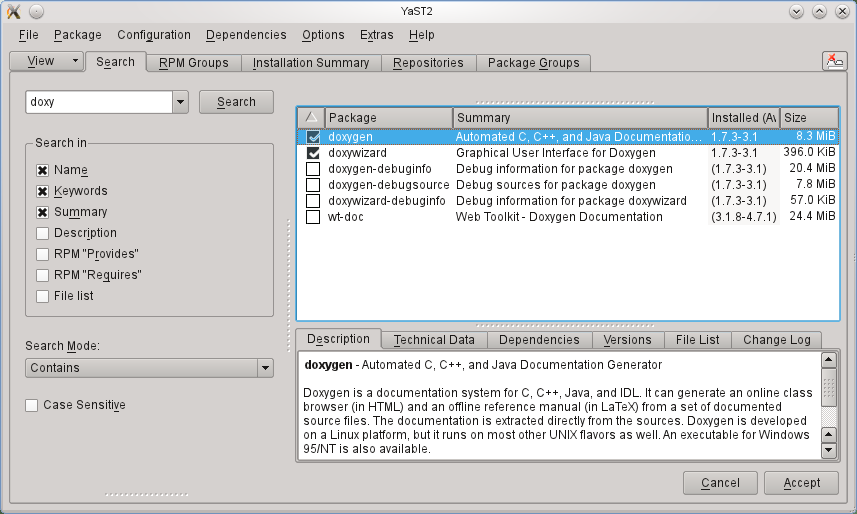
\includegraphics[width=0.75\textwidth]{image/install/OpenSUSE/setup}
\caption[پنجره‌ی نصب برنامه‌ها در سیستم عامل \lr{OpenSUSE}.]{
پنجره‌ی نصب برنامه‌ها در سیستم عامل \lr{OpenSUSE}. پس از جستجوی نام ابزار مورد
نظر خود، آن‌ها را انتخاب کرده و سپس شروع به نصب کنید.
}
\label{image/install/OpenSUSE/setup}
\end{figure}

در صورتی که \lr{doxygen} یا \lr{doxywizard} در نتایج جستجو مشاهده نشد، احتمالا
مخزن مربوط به این نرم‌افزارها در فهرست مخزن‌های سیستم شما وجود ندارد و باید آن
را اضافه کنید. برای این کار ابتدا آدرس یک مخزن که این ابراز را دارد پیدا کنید
سپس در \lr{YaST} به قسمت \lr{Software Repositories} رفته و این آدرس را به فهرست
مخزن‌های سیستم اضافه کنید. پس از آن دوباره نام ابزارها را جستجو کنید و آن‌ها را
نصب کنید.


% در این قسمت نحوه‌ی نصب، روی سیستم عامل های لینوکسی شرح داده می شود.
% محمد هادی منصوری ۹۰/۳/۲
%
% حق نشر 1390-1402 دانش پژوهان ققنوس
% حقوق این اثر محفوظ است.
% 
% استفاده مجدد از متن و یا نتایج این اثر در هر شکل غیر قانونی است مگر اینکه متن حق
% نشر بالا در ابتدای تمامی مستندهای و یا برنامه‌های به دست آمده از این اثر
% بازنویسی شود. این کار باید برای تمامی مستندها، متنهای تبلیغاتی برنامه‌های
% کاربردی و سایر مواردی که از این اثر به دست می‌آید مندرج شده و در قسمت تقدیر از
% صاحب این اثر نام برده شود.
% 
% نام گروه دانش پژوهان ققنوس ممکن است در محصولات دست آمده شده از این اثر درج
% نشود که در این حالت با مطالبی که در بالا اورده شده در تضاد نیست. برای اطلاع
% بیشتر در مورد حق نشر آدرس زیر مراجعه کنید:
% 
% http://dpq.co.ir/licence
%
\section{لینوکس}
\label{install/linux}

\begin{sloppypar}
برای نصب \lr{Doxygen} روی سیستم عامل‌های لینوکسی نیاز به توزیع دودویی مناسب برای سیستم عامل خود دارید. از آدرس 
\url{http://www.doxygen.org/download.html}
 می‌توانید توزیع مناسب را دریافت کنید. پس از دریافت توزیع مناسب، با دستورات زیر می‌توان \lr{Doxygen} را نصب کرد. 
معمولا بین پرونده‌های دریافت شده، پرونده‌ای به نام \lr{configure} وجود دارد. این پرونده حاوی دستورات خط فرمان (دستورات شل) برای 
پیکربندی اولیه است. دستورات زیر پیکربندی اولیه را انجام داده و برنامه را نصب می‌کند.
\end{sloppypar}
\begin{latin}
\lstset{language=C++}  
\begin{lstlisting}[frame=single] 
./configure
make install
\end{lstlisting}
\end{latin}
%\begin{flushleft}
%\lr{./configure} \\
%\lr{make install}
%\end{flushleft}
برای نصب مستندات و مثال‌ها دستور زیر را اجرا کنید.
\begin{latin}
\lstset{language=C++}  
\begin{lstlisting}[frame=single] 
make install_docs
\end{lstlisting}
\end{latin}
%\begin{flushleft}
%\lr{make install\_docs}
%\end{flushleft}
پرونده‌های اجرایی در مسیر 
\lr{<prefix>/bin}
 و مستندات و مثال‌ها در مسیر 
\lr{<docdir>/doxygen}
  نصب می‌شوند.

\begin{sloppypar}
به صورت پیش‌فرض 
\lr{<prefix>}
 به آدرس 
\lr{usr/local}
 اشاره دارد، اما می‌توان آن را با تغییر پارامتر 
\lr{--prefix}
 در پرونده‌ی \lr{configure} تغییر داد. 
\lr{<docdir>}
 نیز به صورت پیش‌فرض به آدرس 
\lr{<prefix>/share/doc/packages}
 اشاره دارد که این آدرس را نیز می‌توان با تغییر پارامتر 
\lr{--doxdir}
 در پرونده‌ی \lr{configure} عوض کرد.
\end{sloppypar}

در صورتی که از بسته‌های \lr{RPM} یا \lr{DEP} استفاده می‌کنید، همان روند استاندارد 
نصب را دنبال کنید که برای این بسته‌ها مورد نیاز است.


% در این قسمت نحوه‌ی نصب DoxyGen روی سیستم عامل ویندوز توضیح داده شده است.
% محمد هادی منصوری. ۹۰/۳/۱
%
% حق نشر 1390-1402 دانش پژوهان ققنوس
% حقوق این اثر محفوظ است.
% 
% استفاده مجدد از متن و یا نتایج این اثر در هر شکل غیر قانونی است مگر اینکه متن حق
% نشر بالا در ابتدای تمامی مستندهای و یا برنامه‌های به دست آمده از این اثر
% بازنویسی شود. این کار باید برای تمامی مستندها، متنهای تبلیغاتی برنامه‌های
% کاربردی و سایر مواردی که از این اثر به دست می‌آید مندرج شده و در قسمت تقدیر از
% صاحب این اثر نام برده شود.
% 
% نام گروه دانش پژوهان ققنوس ممکن است در محصولات دست آمده شده از این اثر درج
% نشود که در این حالت با مطالبی که در بالا اورده شده در تضاد نیست. برای اطلاع
% بیشتر در مورد حق نشر آدرس زیر مراجعه کنید:
% 
% http://dpq.co.ir/licence
%
\section{ویندوز}

در آدرس
\url{http://www.doxygen.org/download.html} 
یک برنامه‌ی اجرایی برای نصب نسخه‌ی ویندوزی وجود دارد. این برنامه به صورت یک
مجموعه کامل قابل نصب است و نصب آن بسیار ساده است.
کافی است پنجره‌های محاوره‌ای را دنبال کنید.



در هنگام نصب در یکی از مراحل از کاربر خواسته می‌شود موارد لازم برای نصب را تعیین کند. 
تصویر \ref{پنجره_نصب_روی_ویندوز} را ببینید. در این مرحله 
فهرستی از ابزارهایی که نصب می‌شودقرار داده شده است. 
همانگونه که در تصویر \ref{پنجره_نصب_روی_ویندوز} دیده می‌شود یکی از ابزارها، \lr{Doxywizard} است. 
به این ترتیب می‌توان در نسخه‌ی ویندوزی، هر دو ابزار \lr{Doxygen} و \lr{Doxywizard} را نصب کرد.

\begin{figure}
\centering
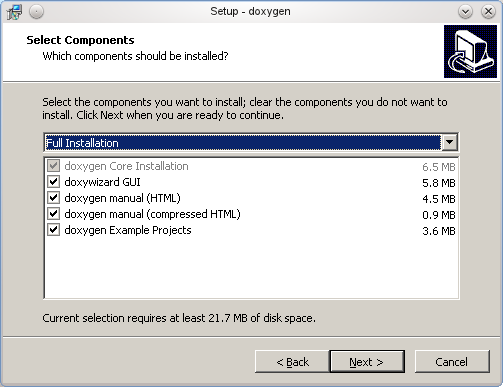
\includegraphics[width=0.75\textwidth]{image/windows_setup}
\caption[
پنجره‌ی محاوره‌ای نصب
{\lr{Doxygen}}
 روی ویندوز
]{
پنجره‌ی محاوره‌ای نصب
{\lr{Doxygen}}
 روی ویندوز. در این پنجره فهرستی از مواردی که باید نصب شود قرار دارد.
}
\label{پنجره_نصب_روی_ویندوز}
\end{figure}

توصیه می شود که بعد از نصب،
\lr{GraphViz} 
(نسخه‌ی ۲/۸ یا جدیدتر) را هم دریافت کرده و نصب کنید.
\lr{Doxygen}
 می تواند از ابزار
\lr{dot}
 مربوط به بسته‌ی
\lr{GraphViz}
، برای تولید بهتر دیاگرام ها استفاده کند.
% تنظیم \lr{HAVE\_DOT} در پرونده‌ی پیکربندی را مشاهده کنید.

اگر می‌خواهید پرونده‌های فشرده‌ی \lr{HTML} تولید کنید، نیاز به 
\lr{Microsoft HTML help} 
دارید. این ابزار را می‌توانید از آدرس 
\url{http://msdn.microsoft.com/en-us/library/ms670169}
 دریافت کنید.
%(تنظیم \lr{GENERATE\_HTMLHELP} را در پرونده‌ی پیکربندی مشاهده کنید)،

اگر می‌خواهید پرونده‌های فشرده‌ی \lr{Qt} را تولید کنید، نیاز به \lr{qhelpgenerator} دارید که قسمتی از \lr{Qt} 
 است. \lr{Qt} را می‌توانید از آدرس 
\url{http://qt.nokia.com/downloads/}
دریافت کنید.

به منظور تولید خروجی \lr{PDF}، یا استفاده از فرمول‌های خاص، احتیاج به نصب
\lr{LaTeX} و \lr{Ghostscript} دارید.
برای \lr{LaTex} چند توزیع وجود دارد. از جمله موارد معروف که باید با \lr{doxygen}
کار کنند \lr{MikTex} و \lr{XemTex} است\footnote{متاسفانه تولید مستند در قالب
\lr{LaTeX} با استفاده از \lr{Doxygen} برای مستندات به زبان فارسی با مشکلاتی
روبروست}.
\lr{Ghostscript} 
 را می‌توان از آدرس
\url{http://sourceforge.net/projects/ghostscript/} 
 دریافت کرد.

پس از نصب \lr{LaTex} و \lr{Ghostscript} باید مطمئن شوید که ابزارهای
\lr{latex.exe}، \lr{pdflatex.exe} و \lr{gswin32c.exe} در مسیر جستجوی دستورات خط
فرمان قرار دارند. در صورتی که از این موضوع مطمئن نیستید دستورالعمل زیر را دنبال
کنید و دستورات را در خط فرمان اجرا کنید تا ببینید به درستی کار می‌کنند یا نه.

از صفحه‌ی اصلی ویندوز روی \lr{My Computer} کلیک راست کرده و گزینه‌ی
\lr{Properties} را انتخاب کنید.
 در پنجره‌ای که ظاهر می‌شود زبانه‌ی \lr{Advanced} را انتخاب کنید. سپس دکمه‌ی
 \lr{Environment Variables} را کلیک کنید.
 در پنجره‌ای که ظاهر می‌شود متغیر \lr{Path} را انتخاب کرده و دکمه‌ی \lr{Edit} را
 کلیک کنید.
 سپس مسیرهای مربوط به ابزارهای گفته شده را در صورتی که وجود نداشت، در این قسمت
 اضافه کنید.
 مسیرهای مختلف با استفاده از علامت نقطه ویرگول از هم جدا می‌شوند. مثلا
\lr{C:\textbackslash Program Files;C:\textbackslash Winnt;C:\textbackslash
Winnt\textbackslash System32}.

پس از انجام کارهای گفته شده نرم‌افزار \lr{Doxygen} نصب شده و آماده استفاده است.


% NOTE : مصطفی 1391 : تشریح نحوه نوشتن
%   در این بخش تنها به بررسی اصول نوشتن مستند پرداخته شده است مستقل از نوع
%   کاربرد آن در استانداردهای متفاوت.

\part{مستند نویسی}
در این بخش، نشان داده می‌شود که چگونه مستند یک برنامه باید ایجاد شود.

%
% حق نشر 1390-1402 دانش پژوهان ققنوس
% حقوق این اثر محفوظ است.
% 
% استفاده مجدد از متن و یا نتایج این اثر در هر شکل غیر قانونی است مگر اینکه متن حق
% نشر بالا در ابتدای تمامی مستندهای و یا برنامه‌های به دست آمده از این اثر
% بازنویسی شود. این کار باید برای تمامی مستندها، متنهای تبلیغاتی برنامه‌های
% کاربردی و سایر مواردی که از این اثر به دست می‌آید مندرج شده و در قسمت تقدیر از
% صاحب این اثر نام برده شود.
% 
% نام گروه دانش پژوهان ققنوس ممکن است در محصولات دست آمده شده از این اثر درج
% نشود که در این حالت با مطالبی که در بالا اورده شده در تضاد نیست. برای اطلاع
% بیشتر در مورد حق نشر آدرس زیر مراجعه کنید:
% 
% http://dpq.co.ir/licence
%
\chapter{مستند کردن پروژه}

%ToDO: maso 1391: یک مقدمه بر این گفتار نوشته شود
در این گفتار نه تنها مستند و انواع آن بلکه روش‌های متفاوت نوشتن مستند و مدیریت
آن بررسی خواهد شد.

از انجا که همواره زبان‌های برنامه سازی شبیه \lr{C/C++} مورد توجه این کتاب است،
تکیه این گفتار به روی ساختارهای مستندسازی در این زبانها است گرچه به زبان‌های
برنامه سازی دیگر نیز اشاره می‌شود.

% TODO: maso 1391: در صورتی که کل کتاب عرف بر این بود که به ساختار گفتار پرداخته
% شود.
 در بخش‌های ابتدای ساختار کلی مستند نویسی آورده می‌شود. در بخش‌های پایانی
چگونگی نوشتن مستند برای موجودیت‌های متفاوت آورده می شود.


\section{مستند و انواع آن}

در زبان‌های برنامه سازی \glspl{comment} یک ساختار برنامه نویسی است که به عنوان
توضیحات خوانا برای برنامه نویسان در لابه لای کدهای برنامه نوشته می‌شود. گرچه این
توضیحات توسط مترجم‌های زبان برنامه سازی نادیده گرفته می‌شود اما برای توسعه
دهندگان سیستم‌های نرم‌افزاری بسیار حیاطی است. هدف اصلی ساختار \glspl{comment} در
زبان‌های برنامه سازی اسان ساختن درک یک برنامه است اما از آنجا که زبان‌های
برنامه‌سازی از ساختارهای دقیقی در کدها پیروی می‌کنند دور از انتظار نیست که در
این مورد نیز ساختارهای از پیش تعریف شده‌ای ایجاد شود.

گرچه استفاده از \glspl{comment} در ساختارهای برنامه سازی منجر به فهم ساده از
برنامه می‌شود اما استفاده نامناسب از آن و ایجاد اطلاعات نامناسب، کم و یا گاها
اضافی منجر به ناکارآمد شدن آن می‌شود. در این راستا راهکارها و توسیه‌های متفاوتی
از سوی تحلیلگران و توسعه‌دهندگان سیستم‌های نرم‌افزاری ارائه شده است که می‌تواند
در این امر بسیار کارساز و مفید باشد.

به هر حال امروز بسیار مرسوم است که با استفاده از \glspl{comment} مستندهای مفید و
جامعی در مورد سیستم‌ها ایجاد شده و در داخل کد برنامه‌ها قرار گیرد\cite{17wiki}.
برای نمونه \glspl{comment} می‌تواند شامل اطلاعاتی مانند توسعه‌دهنده، نسخه، تاریخ
و یا روش‌های به کار رفته در پیاده‌سازی باشد. بزرگترین خصوصیت استفاده از
ساختار \glspl{comment} در مستند کردن کدهای ایجاد شده، ساده‌تر شدن فرآیند
مستندسازی سیستم‌ها است. از سویی نوشتن مستند در کدهای ایجاد شده این امکان را
ایجاد می‌کند که مستند ایجاد شده همواره به روز باشد. در نهایت مستندهای ایجاد شده
در این ساختارها با استفاده از ابزارهای مستندگر سازماندهی شده به شکلهای مناسب در
اختیار کاربران سیستم قرار خواهد کرد.

% maso 1391: انواع مستندها در این قسمت توضیح داده می‌شود
همواره مستندهای موجود در یک ساختار برنامه‌سازی را می‌توان در دو موضوع کلی
دسته‌بندی کرد: مستند فنی و پیاده‌سازی. در بسیاری از موارد بسته‌های نرم‌افزاری
ایجاد شده به عنوان زیر سیستم‌هایی در سایر سیستم‌ها مورد استفاده قرار می‌گیرند.
در این صورت باید مستندهای کافی در مورد ساختار و نحوه به کارگیری ایجاد شود تا
کاربران (که عموما توسعه دهنده هستند) بتواند به صورت کارا از آن استفاده کنند.

از سویی همواره سیستم‌های نرم‌افزاری نیاز به توسعه و رفع ایراد دارند بدیهی است که
در این حالت می‌بایست اطلاعات کافی در مورد روش‌های پیاده‌سازی و محدودیت‌های آن
ایجاد شود. الگوریتم‌های به کار رفته ساختارهای داده‌ای داخلی و یا مشکلاتی که در
توسعه سیستم غیر قابل پرهیز است باید به صورت کامل تشریح شود تا در صورت تغییر
ساختار تیم توسعه حیات سیستم دچار خدشه نشود. تفاوت اساسی میان این نوع مستند و
مستند فنی مخاطب آن است. این نوع مستند تنها توسط توسعه دهندگان سیستم مورد استفاده
قرار می‌گیرد در حالی که مخاطب مستند فنی کاربران سیستم هستند. دور از انتظار نیست
که در برخی موارد نیاز به ایجاد یک نوع اطلاعات در هر دو نوع مستند باشد.

در حالت کلی نمی‌توان مرزی میان این دو نوع مستند تعیین کرد اما نکته‌ای که در هردو
انها مشترک است، ایجاد انها به دست برنامه نویسان است. ان نوع مستندها چه توسط
توسعه دهندگان مورد استفاده قرار گیرد چه کاربران، می‌بایست توسط تیم توسعه ایجاد
شود. ایجاد مستند فنی بر اساس قواعد و استانداردهایی ایجاد می‌شود تا بتواند مستند
مفیدی را برای کاربران ایجاد کرن درحالی که مستند پیاده‌سازی کاملا بر اساس روابط و
ضوابط درون گروهی است. 

%
% حق نشر 1390-1402 دانش پژوهان ققنوس
% حقوق این اثر محفوظ است.
% 
% استفاده مجدد از متن و یا نتایج این اثر در هر شکل غیر قانونی است مگر اینکه متن حق
% نشر بالا در ابتدای تمامی مستندهای و یا برنامه‌های به دست آمده از این اثر
% بازنویسی شود. این کار باید برای تمامی مستندها، متنهای تبلیغاتی برنامه‌های
% کاربردی و سایر مواردی که از این اثر به دست می‌آید مندرج شده و در قسمت تقدیر از
% صاحب این اثر نام برده شود.
% 
% نام گروه دانش پژوهان ققنوس ممکن است در محصولات دست آمده شده از این اثر درج
% نشود که در این حالت با مطالبی که در بالا اورده شده در تضاد نیست. برای اطلاع
% بیشتر در مورد حق نشر آدرس زیر مراجعه کنید:
% 
% http://dpq.co.ir/licence
%
% در ساختار جدید در این بخش بسته‌های مستند در کدهای متفاوت تشریح می‌شود.
% maso 1391
% % در این قسمت به بررسی بسته های ویژه مستند و نحوه پیاده سازی آن در کد ها برای
% % تولید مستند و یکپارچه سازی مستندات فنی که در حین کد نویسی وارد می شود پرداخته
% % خواهد شد.
% % قاسم خان زاده ۹/۲/۱۳۹۰
\section{بسته‌های ویژه مستند}

به طور معمول \glspl{comment} با استفاده از \glspl{comment block} (که
\glspl{stream comment} نامیده می‌شود) یا \glspl{line comment} (که همچنین
\glspl{inline comment} گفته می‌شود) ساختاردهی می‌شود\cite{wiki6}. ساختارهای نحوی
\glspl{comment block} در زبان‌های برنامه سازی، امکان نوشتن
مستند در چندین خط را فراهم می‌کند به گونه‌ای که می‌توان از انواع متفاوت علامت‌ها
مانند فضاهای خالی و خط جدید نیز استفاده کرد. این نوع ساختارها با استفاده از دو
\glspl{delimiter} معرفی می‌شود که یکی \glspl{delimiter} شروع \glspl{comment
block} و دیگری \glspl{delimiter} پایانی در نظر گرفته می‌شود. تمام ساختارهای
ایجاد شده در میان این دو \glspl{delimiter} به عنوان مستند در نظر گرفته می‌شود و
توسط \glspl{compiler} در فرآیند \glspl{compile} نادیده گرفته می‌شود. در بسیار از
زبان‌های برنامه سازی (مانند \lr{MATLAB}) می‌توان این نوع ساختار \glspl{comment
block} را به صورت تو در تو ایجاد کرده در حالی که بسیاری از زبان‌های برنامه سازی
(مانند \lr{java}) این روش را حمایت نمی‌کنند\cite{wiki[7][8][9]}

\glspl{line comment} برخلاف \glspl{comment block} تنها از یک \glspl{delimiter}
برای ایجاد ساختار \glspl{comment} استفاده می‌کند. این نوع مستندها به طور معمول
با یک \glspl{delimiter} شروع شده و تا انتهای خط جاری در نظر گرفته می‌شود. در
برخی از زبان‌های برنامه سازی \glspl{line comment} را حتی از یک ستون تا انتهای خط
در نظر می‌گیرند که در این حالت هیچ \glspl{delimiter}ی مورد استفاده قرار
نمی‌گیرد\cite{wiki9}.

گرچه ممکن است در برخی از زبانهای برنامه سازی تنها یک نوع ساختار \glspl{comment}
مورد حمایت باشد اما در اغلب زبان‌های برنامه سازی، هر دو نوع ساختار
\glspl{comment} پشتیبانی می‌شود. برای نمونه در زبان برنامه سازی \lr{C} با
استفاده از \glspl{delimiter}های \lr{/*} و \lr{*/} \glspl{comment block} و با
استفاده از \lr{//} \glspl{line comment} ایجاد می‌شود در حالی که در زبان برنامه
سازی \lr{Ada} تنها از \glspl{line comment} پشتیبانی می‌شود که با استفاده از
\glspl{delimiter} \lr{--} نمایش داده می‌شود\cite{wiki9}.

در این بخش \glspl{comment block} و \glspl{line comment} در زبان‌های برنامه سازی
متفاوت مورد بررسی قرار خواهد گرفته و نشان داده می‌شود که چگونه می‌توان مستند‌های
فنی و پیاده سازی را با استفاده از آنها ساختاردهی کرد.
\glspl{comment block} کاربردهای متفاوتی دارد و می‌تواند به روش‌های متفاوت و در
مکان‌های متفاوتی ایجاد شود اما در اینجا تنها ساختارهایی مد نظر است که به عنوان
مستندهای فنی ایجاد شده و با استفاده از ابزارهای \glspl{documenter} به قالب‌های
مناسب خروجی تبدیل می‌شود. این نوع ساختارها را می‌توان به عنوان \glspl{comment
block}های خاص در نظر گرفت که در آن با استفاده از توصیف کامل و جامع از اجزای یک
سیستم نرم‌افزاری تلاش می‌شود مستند جامعی از سیستم ایجاد شود. 

از سویی ابزارهای \glspl{documenter} بر اساس ساختارهای معرفی شده در زبان‌های
برنامه سازی روش‌های متفاوتی را برای نوشتن مستند در داخل کد نرم‌افزار ارائه
می‌کنند. این ابزارها بر اساس این ساختارها میان مستندهای فنی و پیاده‌سازی تفاوت
قائل شده و در فرآیند تولید مستند، داده‌های مناسب را از کد استخراج می‌کنند.

\begin{note}
ابزار مورد نظر این کتاب \glspl{doxygen} است از این رو تنها ساختارهای آن مورد
بررسی قرار خواهد گرفت. این ابزار \glspl{documenter} از ساختارهای متفاوتی که در
ابزارهای معادل دیگر استفاده می‌شود حمایت می‌کند از همین رو به عنوان یک ابزار
بسیار قوی در این زمینه مطر است. برای نمونه ابزارهای مانند \lr{JavaDoc} و
\lr{QtDoc} و ساختارهای مورد استفاده آنها نیز مورد حمایت است.
\end{note}

% maos 1381: ساختار مستند جاوا
یکی از ابزارهای قدرتمند \glspl{documenter} \lr{JavaDoc} است که توسط شرکت
\lr{SunMicrosystem} برای زبان برنامه سازی \lr{Java} معرفی شده است. ساختارهای
مناسب \glspl{comment block} در این ابزار، آن را به عنوان محبوب‌ترین ابزار در
زبان برنامه سازی جاوا مطرح ساخته است. در اینجا نیز می‌توان با استفاده از روش
معرفی شده در \lr{JavaDoc} \glspl{comment block}های ویژه خود را معرفی کرد و
مستند‌های مورد نیاز را در آنها به وحود آرود. 
در این روش از دو نشانه \lr{**} برای ایجاد یک \glspl{document block} 
در برنامه استفاده می شود. هر \glspl{comment block} که با \lr{/**} شروع شود به
عنوان یک \glspl{document block} در نظر گرفته می شود و در فرآیند تولید مستند فنی
مورد استفاده قرار می‌گیرد. ساختار کلی \glspl{document block} به صورت زیر است:

\begin{C++}
/**
 * <Document Block>
 */
\end{C++}

در این نمونه قابل مشاهده است که \glspl{document block} با استفاده از نشانه
\lr{/**} شروع شده و در نهایت به نشانه \lr{*/} ختم می‌شود.

\begin{note}
تمام ساختارهای ممکن \glspl{comment} در استاندارد \lr{JavaDoc} به عنوان مستند
پیاده‌سازی در نظر گرفته می‌شود از این رو در ایجاد مستند فنی نهایی مورد استفاده
قرار نخواهد گرفت. اما در اینجا یک استثنا وچود دارد: ابزار \glspl{doxygen} از
استاندارد ابزارهای دیگر مستند سازی نیز حمایت می‌کند از این رو ساختارهای دیگر نیز
وجود دارد که به عنوان مستند فنی در نظر گرفته شود.
\end{note}

% maso 1391: ساختار مستند کیوتی

یکی دیگر از قالب‌هایی که در مستند سازی نرم‌افزارها مورد استفاده قرار می‌گیرد،
ساختارهای معرفی شده در \lr{QtDoc} است که به صورت گسترده در مستند سازی پروژه‌های
\lr{Qt} مورد استفاده قرار می‌گیرد. یکی از مشهورترین پروژه‌هایی که مبتنی بر
\lr{Qt} بوده و به صورت گسترده از قراردادهای \lr{QtDoc} در مستند سازی خود استفاده
می‌کند \lr{KDE} است. ساختارها و قرادادهای مورد استفاده در \lr{QtDoc} نیز در
اینجا مورد حمایت است. در این قرارداد از عبارت \lr{/*!} برای ایجاد
\glspl{document block} استفاده می‌شود و در نهایت به عبارت \lr{*/} ختم می شود.
ساختار کلی \glspl{document block} به صورت زیر است.

\begin{C++}
/*!
 * <Document Block>
 */
\end{C++}

با یک نگاه کوتاه به این ساختار شباهیت میان آ‌ن با ساختارهای
معرفی شده در \lr{JavaDoc} نمودار می‌شود. به هر حال در قراردادهای \glspl{doxygen}
از هردو این ساختارها حمایت می‌شود و توسعه دهنده سیستم مختار است در مواقع مورد
نیاز از آنها استفاده کند.

\begin{note}
استفاده از نشانه \lr{*} ابتدای هر خط در \glspl{document block} اختیاری است و
معمولا برای زیبایی ظاهری مستند‌های ایجاد شده مورد استفاده قرار می‌گیرد. به عنوان
نمونه تک کد زیر نیز یک ساختار معتبر در نظر گرفته می‌شود.

\begin{C++}
/*!
   <Document Block>
 */
\end{C++}

بسیاری از ابزارهای \glspl{code beautifier} تلاش می‌کنند با قرار دادن این نشانه
ابتدای هر خط ساختار مناسبی را در کدهای نوشته شده ایجاد کنند. این نشانه‌ها در
مستند نهایی تولید شده حذف خواهد شد.
\end{note}

در بسیاری از موارد مستند کوتاه بوده لذا نیازی به استفاده از \glspl{comment
block} نیست. در این موارد می‌توان از ساختارهای \glspl{line comment} استفاده
کرد. ساختار کلی \glspl{comment block} با استفاده از ساختارهای \glspl{line
comment} به صورت زیر است.

\begin{C++}
///
/// <Document Block>
///
\end{C++}

این ساختار با توجه به قرادادهای \lr{QtDoc} نیز به فرم زیر خواهد بود.

\begin{C++}
//!
//! <Document Block>
//!
\end{C++}

در این ساختارها از به ترتیب از نمادهای اضافی \lr{/} و \lr{!} برای ایجاد تمیز
میان \glspl{comment block} و مستند پیاده سازی استفاده شده است. توجه به این نکته
الزامی است که در این ساختار ابتدای هر سطر از \glspl{comment block} الگو ثابتی
تکرار می‌شود.

برخی از برنامه نویسان علاقه دارند که مستندهای فنی خود را به گونه‌ای خاص متمایز
از سایر مستندهای دیگر ایجاد کنند. برای نمونه در بسیاری از پیاده‌سازی‌های
مستندهای فنی به صورت زیر ایجاد شده است.

\begin{C++}
/***********************************************
 *  <Document Block>
 ***********************************************/
\end{C++}

برای حمایت از این دسته برنامه نویسان این ساختار نیز در \glspl{doxygen} مورد
حمایت قرار گرفته است. البته مشابه به همین ساختار نیز می‌توان از \glspl{line
comment} نیز استفاده کرد که ساختار کلی آن به صورت زیر است.

\begin{C++}
/////////////////////////////////////////////////
/// <Document Block>
/////////////////////////////////////////////////
\end{C++}


\begin{ebox}% maso 1391: مستند سازی سایر زبانهای برنامه سازی
زبانهای برنامه سازی متفاوتی مانند \lr{Pyton}، \lr{VHDL} و \lr{Fortran} نیز با
استفاده از \glspl{doxygen} مورد حمایت هستند. در این زبان‌ها از ساختارهای متفاوتی
برای ایجاد \glspl{comment block} استفاده می شود.

در زبان برنامه سازی \lr{VHDL} \glspl{comment} با استفاده از یک \lr{-} معرفی
می‌شود از این رو در \glspl{doxygen} با استفاده از نشانه \lr{-!} \glspl{comment
block} را مشخص می‌کند. با استفاده از این روش نه تنها می‌توان مستندها را در یک خط
بلکه به صورت چند خطی نیز ایجاد کرد. به این نکته باید توجه داشته که در مستندهای
چند خط این نشانه ابتدای هر خط باید قرار گیرد.

\glspl{comment block}ها در این زبان برنامه سازی همواره پیش از قسمت‌های مورد نظر
آورده می‌شود. اما تنها یک استثنا وجود دارد و آنهم در مورد \glspl{vhdl:port} است.
\glspl{comment block} در این مورد می‌تواند بعد از تعریف \glspl{vhdl:port}
آورده شود و به عنوان یک توصیف کوتاه از آن در نظر گرفته شود.


زبان برنامه سازی \lr{Fortran} تنها از \glspl{line comment} حمایت می‌کند که با
استفاده از نشانه‌های \lr{*}، \lr{C} یا \lr{!} ابتدای خط ایجاد می‌شود.
\glspl{doxygen} از عبارت‌های \lr{!>} یا \lr{!<} یک \glspl{document block} ایجاد
می‌شود. عبارت‌های \lr{!>}‌و \lr{!!} نیز برای ایجاد مستند در چندین خط مورد
استفاده قرار می‌گیرد.

زبان برنامه سازی \lr{Tcl} نیز یکی دیگر از زبان‌های پرکاربرد است که توسط
\glspl{doxygen} پشتیبانی می‌شود. در این زبان برنامه سازی مستندها تنها به صورت
\glspl{line comment} پشتیبانی می‌شود. از این رو \glspl{document block} با
استفاده از \lr{\#\#} از دیگر \glspl{comment block}ها تمییز داده می‌شود. در این
زبان برنامه سازی هر \glspl{document block} با رسیدن به اولین خط که با \lr{\#}
شروع نشود پایان می‌یابد.

زبان برنامه سازی \lr{Python} نیز جایگاه خاصی در زبان‌های برنامه سازی دارد. در
این زبان برنامه‌سازی از یک گونه خاص مستند استفاده می‌شود که
\glspl{pyton:documentation string} نامیده می‌شود. در این زبان برنامه سازی با
استفاده از \glspl{pyton:documentation string}ها روش منحصر به فردی در ایجاد مستند
فنی پایه ریزی شده است. به هر حال \glspl{doxygen} با استفاده از متن‌های
\glspl{pyton:documentation string} مستند فنی نهایی را ساختاردهی خواهد کرد. علاوه
بر این در این زبان برنامه سازی از سازکار مشابه به زبان برنامه سازی \lr{Tcl} در
ساختار \glspl{comment} استفاده می‌شود. در اینجا نیز \glspl{document block} با
استفاده از نشانه \lr{\#\#} مشخص می‌شوند.
\end{ebox}

\subsection{مستند بعد از عضو}

اگر هدف مستند کردن اعضای یک فایل، ساختار، کلاس یا ساختارهای باشد که از اجزای
متفاوتی تشکیل شده اند (مانند \lr{enum})، بهترین روش نوشتن  مستند هر بخش درست
جایی است که تعریف شده است. در \glspl{doxygen} امکان نوشتن \glspl{document block}
بعد از تعریف یک موجودیت فراهم شده است. ساختار کلی \glspl{document block} بعد از
اجزا به صورت زیر است.

\begin{C++}
<Definition>; /**< <Document block> */
\end{C++}

در این ساختار تنها نشانه \lr{<} به ساختار \glspl{document block} اضافه شده است.
بدیهی است که با اضافه کردن این نشانه به دیگر ساختارهای \glspl{document block}
نیز بتوان از آنها نیز بهره برد. برای نمونه در زیر کدی آورده شده است که ساختارهای
متفاوت برای ایجاد \glspl{document block} بعد از تعریف اجزای یک ساختار داده‌ای
مورد استفاده قرار گرفته است.

\begin{C++}
struct {
	int var; /*!< Description */
	int var; /**< Description */
	int var; //!< Description
	         //!< 
	int var; ///< Description
	         ///<
	int var; //!< Description
	int var; ///< Description
}
\end{C++}

از این روش حتی برای نوشتن مستند پارامترهای ورودی توابع نیز استفاده می‌شود. در کد
زیر یک تابه به نام \lr{foo} تعریف شده که دارای یک پارامتر به نام \lr{v} است. این
پارامتر به عنوان ورودی در نظر گرفته می‌شود. مستند کامل این پارامتر بعد از تعریف
آن آورده شده است.

\begin{C++}
void foo(int v /**< [in] docs for input parameter v. */);
\end{C++}

باید یادآور شد که ساختار این \glspl{document block} مشابه است و معنی آنها مانند
\glspl{document block}هایی است که پیش از این آورده شده است. تنها
تفاوت آنها این است که نشانه \lr{<} در ابتدای آن ها می‌آید و هدف آن قرار دادن
مستند بعد از تعریف اجزای برنامه نویسی است.

در زیر یک نمونه از مستند شده است که شامل تمام مفاهیمی است که تا کنون بیان شده
است.

\begin{C++}
/*! A test class */
class Test
{
  public:
    /** An enum type. 
     *  The documentation block cannot be put after the enum! 
     */
    enum EnumType
    {
      int EVal1,     /**< enum value 1 */
      int EVal2      /**< enum value 2 */
    };
    void member();   //!< a member function.
    
  protected:
    int value;       /*!< an integer value */
};
\end{C++}

\subsection{مستند در مکان های دیگر}

همانطور که در توضیحات بخش قبل آمد، بسته های مستند همیشه در جلوی تعریف یک فایل،
کلاس، یا فضای نام یا در جلوی عضوهای آن می آیند.
یکی از مواری که می تواند به نوشتن مستندهای یک برنامه، ساختاری منظم بدهد، نوشتن
مستندها در جایی غیر از کدهای نوشته شده است. با استفاده از این روش می توان کدها
را در یک فایل و مستندهای مربوط به همان کدها را در فایلی جداگانه نوشت و مستند هر
قسمت را به آن ارجا داد.

\glspl{doxygen} به شما امکان می دهد بسته های مستند را بصورت تجربی هر جایی که می
خواید بگذارید. هزینه‌ٔای که شما برای نگذاشتن بسته مستند بطور مستقیم قبل یا بعد
از یک عنوان می‌پردازید این است که باید مجموعه‌ای از دستورات ساخت یافته را در داخل بسته مستند
قرار دهید. این کار منجر به تکرار اطلاعات می شود.بنابراین جهت پیاده سازی یک
\glspl{document block}، در صورت امکان از دستورهای ساختاری استفاده نکنید مگر
اینکه نیاز به چنین کاری احساس شود.

%
% حق نشر 1390-1402 دانش پژوهان ققنوس
% حقوق این اثر محفوظ است.
% 
% استفاده مجدد از متن و یا نتایج این اثر در هر شکل غیر قانونی است مگر اینکه متن حق
% نشر بالا در ابتدای تمامی مستندهای و یا برنامه‌های به دست آمده از این اثر
% بازنویسی شود. این کار باید برای تمامی مستندها، متنهای تبلیغاتی برنامه‌های
% کاربردی و سایر مواردی که از این اثر به دست می‌آید مندرج شده و در قسمت تقدیر از
% صاحب این اثر نام برده شود.
% 
% نام گروه دانش پژوهان ققنوس ممکن است در محصولات دست آمده شده از این اثر درج
% نشود که در این حالت با مطالبی که در بالا اورده شده در تضاد نیست. برای اطلاع
% بیشتر در مورد حق نشر آدرس زیر مراجعه کنید:
% 
% http://dpq.co.ir/licence
%
% تعریف و سازماندهی مستند در این بخش ساختار کلی مستندها اورده می‌شود به بیان
% دیگر بیان می‌شود که متن مستند چگونه سازماندهی شده و نوشته می‌شود. چگونگی
% استفاده از برچسب‌ها و تعریف آنها و یا ایجاد پاراگراف و قسمت اشاره می‌شود.

\section{ساختار مستند}

پیش از این بیان شد که با استفاده از ساختارهای خاض دسته‌ای از \glspl{comment
block}ها به عنوان \glspl{document block} در نظر گرفته می‌شود. ابزارهای
\glspl{documenter} بر اساس \glspl{document block}های ایجاد شده مستند فنی کلی
سیستم را ساختاردهی و ایجاد می‌کنند. گرچه ساختاردهی و ایجاد مستند نهایی می‌تواند
به صورت خودکار ایجاد شود اما با ایجاد راهکارهای مناسب می‌توان امکاناتی جهت
مدیریت مستند فنی تولید شده توسط این ابزارها را بهبود بخشید. از این رو در بسیاری
از ابزارهای \glspl{documenter} نه تنها الگو و ساختارهایی برای \glspl{document
block} ارائه می‌شود بلکه دسته‌ای از دستورها و تنطیم‌ها برای مدیریت آنها نیز در
نظر گرفته می‌شود.

% FIXME: maso 1391: ساختار کلی بسته‌های مستند و رابطه آنها
% در این قسمت باید این ساختارها به صورت کامل تشریح شود. برای نمونه همواره پیش از
% هر موجودیت برنامه سازی مستند وارد می‌شود.

معمولا یک برنامه از بلاک های مختلفی تشکیل شده است. بطور مثال یک برنامه می تواند
شامل بلاک یک تابع، بلاک یک کلاس، بلاک یک متغیر و ... باشد. حال این توضیحات شامل
الحاق همه بلاک های توضیحاتی است که در یک تابع یا متد آورده شده است. بدین ترتیب
می توان تمام عبارت های وارد شده در کد که بصورت جدا از هم قرار دارند را به یکدیگر
متصل کرد. توصیف های مختصر معمولا بیان کننده توصیفات کلی یک بلاک از برنامه می
باشد. همچنین توصیف های مختصر مانند یک نام پیشنهادی، یک توصیف خلاصه،یک خط کوتاه
توضیح است که توصیف کننده کلی یک بخش از مستنداتی است که در آینده به کدها اضافه می
شود. توصیف های مختصر همچنین می توانند شامل مجموعه ای از توضیحات خلاصه یا توصیف
گر یک مجموعه از جزئیات پیاده سازی شده باشند. یادآور می شود که داشتن بیش از یک
توصیف خلاصه یا جزئیات مجاز می باشد(البته استفاده از این روش توصیه نمی شود).

\begin{note}
همانگونه که در بخش \ref{write/document-the-code/comment-block} گفته شد، به
روش‌های متفاوتی می‌توان یک \glspl{document block} را ایجاد کرد. در ادامه همواره
از یک روش یکتا برای ایجاد \glspl{document block} استفاده می‌شود که به صورت زیر
است:

\begin{Java}
/**
 * <Docuemnt block>
 */
\end{Java}

این به آن معنی نیست که دیگر ساختارهای مورد استفاده در ایجاد یک \glspl{document
block} معتبر نیست. از این رو می‌توان این روش را با هر روش دیگری جایگزین کرد. هدف
اصلی از این کار یک نواخت بودن ساختار کتاب است.
\end{note}

 مستندهای که در یک  \glspl{document block} وارد می شود را می‌توان بطور کلی به دو
دسته کلی تقسیم: توصیف کلی و توصیف جزئی. به طور معمول هر \glspl{document block}
با یک توصیف جزئی شروع شده و در ادامه به صورت مفصل به توصیف اجزای برنامه سازی
می‌پردازد. گرچه ایجاد این دو دسته مستند در \glspl{document block} کاملا اختیاری
است اما برخورد \glspl{documenter}ها با این مستندها متفاوت است. برای نمونه ابزار
\lr{JavaDoc} در گام نخست توصیف کوتاه از هر \glspl{document block} را تعیین کرده
و باقی مانده را به عنوان مستند کلی در نظر می‌گیرد در حالی که این روند در ابزاری
مانند \glspl{CDoc} کاملا برعکس است. این درحالی است که \glspl{doxygen} در این
مورد پویا بوده و بر اساس تنظیم‌های متفاوت می‌تواند روش‌های متفاوتی را به کار
گیرد. 

مستند جزئی عبارت است از یک توصیف کوتاه که به توصیف یک جز برنامه سازی می‌پردازد.
ابزارهای \glspl{documenter} متفاوت راهکارهای متفاوتی را برای تعیین یک مستند جزئی
دنبال می‌کنند. برای نمونه \lr{JavaDoc} پاراگراف نخست از هر \glspl{document
block} را به عنوان مستند جزئی در نظر می‌گیرد در حالت که در \lr{CDoc} و یا
\lr{QtDoc} از برچسب‌ها برای اینکار استفاده می‌شود.

برخلاف مستند جزئی که بسیار کوتاه و خلاصه است، مستند کلی به تشریح کامل یک برنامه
پرداخته و خود به بخش‌های متفاوتی تقسیم می‌شود. این مستند گاها شامل مثال بوده و
به قسمت‌های دیگر برنامه ارجاع دارد. بسته به میزان مستند سازی سیستم این قسمت
می‌تواند از بین چند خط تا چند بخش و زیر بخش متفاوت باشد. ساختار کلی مستند جزئی و
کلی در یک \glspl{document block} بر اساس استانداردهای \lr{JavaDoc} در زیر آورده
شده است.

\begin{Java}
/**
 * <Brief Document>
 *
 * <Detail Document>
 */
\end{Java}

ساختار مورد استفاده در \lr{JavaDoc} بسیار ساده است. در ساختارهای دیگر از
\glspl{doxygen:tag} برای تعیین مستند جزئی و کلی استفاده می‌شود که در ادامه به آن
پرداخته خواهد شد.

بسته ویژه مستند، یک بسته توضیحات در برنامه تویسی \lr{C/C++} با تعدادی علامت
گذاری اضافی است که \lr{doxygen} توسط آن ها تشخیص می دهد این قسمت از کد یک بخش از
مستندی است که در نهایت برای تولید گزارش از آن استفاده می شود.

برای مستند هایی که  خروجی آنها بصورت \lr{HTML} است، توصیف های خلاصه، بصورت
راهنمای ابزار \lr{(tooltip)}  مورد استفاده قرار می گیرد. در این روش قسمت های
مورد نظر از یک مستند، توضیحات آن قسمت از مستند وقتی که توسط موشواره اشاره می
شوند به نمایش در می آید.

% FIXME: maso 1391: تعریف برچسب باید آورده شود.
% برچسب برای تعیین یک دستور است. این کار به روش های متفاوت انجام می‌شود که باید در
% اینجا مورد بررسی قرار گیرد.

همانطور که بیان شد برای ارایه یک توضیح کلی برای یک بلاک از برنامه از توصیف خلاصه
استفاده می شود. برای پیاده سازی این گونه از توصیفات چندین روش وجود دارد که در
زیر بررسی می شود.

یکی از روش های توصیف خلاصه استفاده از فرمان \lr{\textbackslash{brief}} در ابتدای
یک بسته توضیح است. با استفاده از فرمان فوق می توان یک توصیف خلاصه از یک پاراگراف
را در ابتدای توضیحات آورد.

برای کلاس ها و پوشه ها، توصیف خلاصه در لیستی که در ابتدای مستندات یک صفحه آورده
می شود مورد استفاده قرار می گیرد. گستردگی یک توصیف خلاصه ممکن است از چند خط
فراتر رود. (البته تاکید می شود که توصیف خلاصه بیشتر از چند کلمه نباشد.)


\begin{C++}
/*! \brief Brief description.
 *         Brief description continued.
 *
 *  Detailed description starts here.
 */
\end{C++}

بطور معمول بعد از بیان یک خلاصه از جزئیات یک بلاک، موارد دیگری همچون نام
نویسنده، شماره ویرایش، تاریخ، خطاهای احتمالی، نسخه های پیشین، اخطارها و
استاندارد های پیاده سازی شده آورده می شود. البته موارد فوق زمانی مفید است که
توصیف یک کلاس یا پوشه مد نظر باشد وبرای موارد دیگر مانند توصیف متدها و توابع سعی
می شود از موارد دیگر بجز خلاصه استفاده نشود. مانند مثال زیر:

\begin{C++}
/*!
 * \brief Pretty nice class.
 *
 * This class is used to demonstrate a number of section commands.
 * 
 * \author Mostafa Barmshory
 * \version   4.1a
 * \date Aban 1391
 * \copyright GPL
 */
class SomeNiceClass {..};
\end{C++}

ابتدا باید یادآوری کرد که فایل پیکر بندی در مستند نویسی طبق استانداردهای
\lr{doxygen} فایلی است که در آن کلیه ساختار یک مستند و تنظیمات مربوط به مستند در
آن تعریف می شود.

اگر در فایل پیکر بندی تگ  \lr{JAVADOC-AUTOBRIEF} به \lr{yes} نشانده شود آنگاه
بسته های توضیح با قالب \lr{JavaDoc} بصورت پیش فرض و خودکار، خط اول از توضیحات را
تا رسیدن به اولین نقطه و پس از آن یک فضای خالی یا رفتن به سطر بعد را به عنوان
توصیف خلاصه در نظر می گیرد.
در توضیحات \lr{C++} نیز به همین ترتیب عمل می شود.به مثال های زیر دقت کنید.

\begin{C++}
/** Brief description which ends at this dot. Details follow
 *  here.
 */
\end{C++}

سومین مورد استفاده از توصیف های خلاصه درقالب \lr{C++} هنگامی است که یک
توضیح بیشتر از یک خط نیست. در این روش همه توصیف ها در یک خط می آید. مانند مثال
های زیر:

\begin{C++}
/// Brief description.
/** Detailed description. */

//! Brief description.

//! Detailed description
//! starts here.
\end{C++}

توجه کنید که خط خالی آمده در مثال آخر در جایی می آید که نیاز به جدا سازی توصیف
خلاصه از بسته شامل توصیف جزئیات باشد.
برای تنظیم چنین مواردی باید در فایل پیکر بندی باید تگ \lr{JAVADOC-AUTOBRIEF} به
\lr{no} نشانده شود.

همانطور که مشاهده شد در استفاده از توصیفات جزئیات \lr{doxygen} کاملا انعطاف پذیر
است. اگر چندین توصیف جزئیات وجود داشته باشد، همه آنها به هم الحاق خواهند شد.
اگر چندین توصیف جزئیات وجود داشته باشد که باید آنها را جدا از هم در مستند
بیاورید باید هر کدام از آنها را بصورت توضیحات خلاصه در خط های جداگانه قرار دهید.
مانند مثال زیر:

\begin{C++}
//! Brief description, which is
//! really a detailed description since it spans multiple lines.
/*! Another detailed description!
*/
\end{C++}

برخلاف بیشتر سیستم های مستند نویسی دیگر، در \lr{doxygen}  این امکان وجود دارد که
مستند مربوط به یک عضو در جلوی تعریف آن آورده شود. این روش مستند نویسی از این نظر
مفید است که می توان توضیحات را در فایل منبع بجای فایل سرآیند برای یک عضو از
برنامه آورد. این روش مستند نویسی باعث می شود که فایل سرآیند همیشه یکپارچگی خود
را حفظ کند.

گذاشتن مستندات بعد از عضوها:
توصیف های خلاصه بطور کلی بیان کننده یک دید کلی از یک کلاس ، فضای نام یا یک پوشه
هستند. بصورت پیش فرض فونت این قسمت بصورت ضخیم تر نمایش داده می شود(این توصیف می
تواند با نشاندن \lr{BRIEF-DESC} به \lr{no}درفایل پیکربندی پنهان شود.) هر دو مورد
توصیف های خلاصه و یا جزئیات برای قالب \lr{Qt} اختیاری هستند.

بصورت پیش فرض یک بسته مستند با قالب \lr{javaDoc} شبیه به یک قالب مستند \lr{Qt}
رفتار می کند.
این مورد طبق ویژگی های موجود در \lr{javaDoc} نیست،اما جمله اول از بسته مستند
بصورت خودکار مانند یک توصیف خلاصه رفتار می کند.
برای فعال کردن این خصوصیت باید
\lr{JAVADOC-AUTOBRIEF} را در فایل پیکربندی به \lr{yes} بنشانید. اگر شما این
خصوصیت را فعال کنید و بخواهید یک نقطه در بین یک جمله بدون پایان آن بگذارید،
باید یک اسلش و یک فاصله را بعد از ان قرار دهید. به مثال زیر نگاه کنید.

\begin{C++}
/** Brief description (e.g.\ using only a few words). Details follow. */
\end{C++}

بطور مشابه اگر بخواهید جمله اول از یک بسته مستند در قالب \lr{Qt} بصورت خودکار
مانند یک توصیف خلاصه رفتار کندباید \lr{QT-AUTOBRIEF} را درفایل پیکربندی
به\lr{yes} بنشانید.

\lr{doxygen} به شما اجازه می دهد تا مستندهای اعضا(شامل تابع های عمومی) در جلوی
تعریف آن \lr{definition} گذاشته شود. این روش در مستند سازی می تواند در فایل منبع
به منظور استفاده در فایل سرآیند قرار گیرد. این کار باعث می شود که فایل سرآیند
خاصیت یکپارچگی خود را حفظ کند و به مجری عضوها اجازه دسترسی مستقیم به مستند را
دهد. توصیف خلاصه قبل از اعلان عضو و توصیف جزئیات قبل از تعریف عضو قرار داده می
شود.



دستورهای ساخت یافته (مانند تمام دستورهای دیگر در مستند نویسی \lr{doxygen}) با یک
بک اسلش (\textbackslash) dh اتساین (@) شروع می شوند.
در ادامه این دستورات با یک نام دستور و یک یا چند پارامتر ادامه می یابد.

بطور مثال دستور استفاده شده جهت نشان دادن بسته مستند یک کلاس بصورت
\lr{\textbackslash class}
است. در زیر چند دستور که برای ساخت بسته مستند در مکان دیگر استفاده می شود آورده
شده است.

\begin{C++}
\struct to document a C-struct.
\union to document a union.
\enum to document an enumeration type.
\fn to document a function.
\var to document a variable or typedef or enum value.
\def to document a #define.
\typedef to document a type definition.
\file to document a file.
\namespace to document a namespace.
\package to document a Java package.
\interface to document an IDL interface.
\end{C++}

برخی از دستورهای یاد شده دارای یک یا چند آرگومان هستند. هر آرگومان یک محدوده خاص دارد.

\begin{itemize}
  \item     If <sharp> braces are used the argument is a single word.
  \item     If (round) braces are used the argument extends until the end of the line on which the command was found.
  \item     If {curly} braces are used the argument extends until the next paragraph. Paragraphs are delimited by a blank. line or by a section indicator.
\end{itemize}

البته باید یادآور شد که این دستورات بسیار کاملتر هستند.
در پیوند \cite{doxycommand} می توانید به دستورات کامل این مجموعه دست یابید.

دوباره یادآوری می شود برای شی های عمومی (تابع ها،توع های داده ای،توع شمارشی،
ماکروهاو...) مستند باید در همان فایلی که تعریف می شوند قرار گیرند.

\begin{C++}
/*! \file */

or a

/** @file */
\end{C++}

طبق مثال زیر می توان مستندهای یک فایل را بطور جداگانه از خود فایل پیاده سازی
کرد.همانطور که در مثال زیر مشخص است وقتی که مستند های یک فایل منبع  خارج از
خودفایل منبع تعریف می شوند امضای تمام توابعی که قرار است مستند آن ها جداگانه
آورده شود در فایل مستند قرار می گیرد. ضمنا برای مستند کردن هر قسمت از یک فایل
منبع که می تواند شامل کلاس، تابع، متغیر و... باشد دارای یک تگ مربوط  به خود است.
مثلا برا مستند کردن تابع از تگ \lr{/fn}، برای مستند کردن یک ماکرو ازتگ
\lr{/def} برای مستند کردن یک فایل از تگ \lr{/file} و برای مستند کردن یک متغیر
از تگ \lr{/var} استفاده می شود. به دلیل اینکه هر بسته توضیح شامل دستورات
ساختاری است، همه بسته های توضیح می توانند به جای دیگری یا یک فایل ورودی
انتقال یابند (مانند یک فایل حاوی منبع) بدون اینکه بر روی مستندات تولید شده تاثیر
داشته باشند. یکی از معایب استفاده از این روش این است که الگوها ممکن است جایگزین
یکدیگر شوند و یا بازنویسی شوند.

\begin{C++}
/*! \file structcmd.h
\brief A Documented file.

Details.
*/

/*! \def MAX(a,b)
\brief A macro that returns the maximum of \a a and \a b.

Details.
*/

/*! \var typedef unsigned int UINT32
\brief A type definition for a .

Details.
*/

/*! \var int errno
\brief Contains the last error code.

\warning Not thread safe!
*/

/*! \fn int open(const char *pathname,int flags)
\brief Opens a file descriptor.

\param pathname The name of the descriptor.
\param flags Opening flags.
*/

/*! \fn int close(int fd)
\brief Closes the file descriptor \a fd.
\param fd The descriptor to close.
*/

/*! \fn size_t write(int fd,const char *buf, size_t count)
\brief Writes \a count bytes from \a buf to the filedescriptor \a fd.
\param fd The descriptor to write to.
\param buf The data buffer to write.
\param count The number of bytes to write.
*/

/*! \fn int read(int fd,char *buf,size_t count)
\brief Read bytes from a file descriptor.
\param fd The descriptor to read from.
\param buf The buffer to read into.
\param count The number of bytes to read.
*/
#define MAX(a,b) (((a)>(b))?(a):(b))
typedef unsigned int UINT32;
int errno;
int open(const char *,int);
int close(int);
size_t write(int,const char *, size_t);
int read(int,char *,size_t);
\end{C++}


\subsection{تشریح یک بسته مستند}

در بخش قبل به بررسی نحوه وارد کردن مستند در کد با استفاده از استاندارد
\lr{doxygen} پرداختیم. همچنین در مورد اختلاف بین توصیف های خلاصه و جزییات  توضیح
داده شد. بعلاوه درباره استفاده از مستندهای ساخت یافته مطالبی بیان شد.

در این بخش به بررسی محتویات خود بسته مستند پرداخت می شود.
در \lr{Doxygen} از قالب های مختلف مستندات حمایت می شود.
در ساده ترین شکل می توان از متن ساده استفاده کرد. مورد یاد شده برای یک توصیف
کوتاه ایده آل می باشد.
برای بیان توصیف های بزرگتر اغلب به ساختارهای بیشتری نیاز پیدا خواهد شد. این
ساختارها می توانند شبیه یک بسته متن، یک لیست یا یک جدول ساده باشد.

\lr{doxygen} از قالب \lr{Markdown} ، که شامل بخش های توسعه یافته \lr{Markdown
Extra} می باشد، استفاده می کند.
\lr{Markdown} طوری طراحی شده است که برای خواندن و نوشتن بسیار آسان است.
\lr{Doxygen} همچنین خواندن بطور مستقیم از فایل های \lr{Markdown} را پشتیباینی می
کند.
برای کسب اطلاعات بیشتر به آدرس زیر مراجعه شود.

\href{http://www.stack.nl/~dimitri/doxygen/markdown.html}{markdown}

% \glspl{doxygen:tag}‌های در این قسمت تشریح می‌شود که برای نوشتن متن مستقل از خود جای آن و منظور
% آن نوشته می شود

\section{متن مستند}

دسته‌ای از \glspl{doxygen:tag}‌ها برای ایجاد متن‌های متفاوت مورد استفاده قرار می‌گیرد. هدف
اصلی استفاده از این \glspl{doxygen:tag}‌ها زیبا کردن متن مستند است و کاربرد دیگری ندارد. برای
نمونه نوشتن یک متن با قلم‌های زخیم‌تر نمونه‌ای از این کاربردها است. علاوه بر این
نیز دسته‌ای از برچبس‌ها برای الحاق تصویر مورد استفاده قرار می‌گیرد. در این بخش به بررسی
پرکاربردترین \glspl{doxygen:tag}‌های پرداخته شده است که در این نوع کاربردها مورد استفاده قرار
می‌گیرد.

% Text em p c a 

برای نمایش یک کلمه با قلم‌های زخیم‌تر (که معمولا برای نمایش واژه‌های کلید مورد
استفاده قرار می‌گیرد) از \glspl{doxygen:tag} \lr{em} استفاده می‌شود. ساختار کلی
این \glspl{doxygen:tag} به صورت زیر است.

\begin{doxygen}
\em <word>
\end{doxygen}

برای نمایش چندین واژه به عنوان واژه‌های مهم نمی‌توان از این \glspl{doxygen:tag}
یا معادل با آن استفاده کرد. کاربرد این \glspl{doxygen:tag} تنها زمانی که است که
یک واژه مد نظر باشد. برای نمایش چندین واژه با استفاده از قلم‌های زخیم‌تر می‌توان
از ساختار زیر استفاده کرد.

\begin{doxygen}
<tt> Multi Emphasize Words </tt>
\end{doxygen}

در بسیار از موارد نیاز است که در متن مستند به پارامترهای ورودی توابع اشاره کرد.
در این حالت سعی می‌شود نام پارامترها از دیگر واژه‌ها متفاوت باشد.
در این موارد نه تنها می‌توان از \lr{em} بلکه از \glspl{doxygen:tag}هایی مانند
\lr{p} و  \lr{a} نیز استفاده کرد. این \glspl{doxygen:tag}ها به ترتیب تداییگر
واژه‌های \lr{parameter} و \lr{argument} است.

\begin{note}
استفاده از \lr{a}، \lr{p} و \lr{em} همگی مشابه به یک دیگر بوده و لزومی ندارد
که پارامتر ورودی این \glspl{doxygen:tag}‌ها نام یک پارامتر از تابع باشد.
\end{note}

نه تنها \glspl{doxygen:tag} \lr{em} بلکه تمام \glspl{doxygen:tag}‌های معادل آن با استفاده از روش مشابهی
واژه‌های ورودی را متمایز از دیگر واژه‌ها نمایش می‌دهند. یکی دیگر از \glspl{doxygen:tag}‌ها که
تنها برای نمایش زخیم‌تر یک واژه مورد استفاده قرار می‌گیرد \glspl{doxygen:tag} \lr{b} است که
خلاصه شده \lr{bold} است. ساختار کلی این \glspl{doxygen:tag} نیز به صورت زیر است.

\begin{doxygen}
\b <word>
\end{doxygen}

در اینجا نیز برای نمایش چندین واژه به صورت ذخیم‌تر می‌توان از ساختار زیر استفاده
کرد.

\begin{doxygen}
<b> Multi Emphasize Words </b>
\end{doxygen}

% TODO: maso: یک نمونه کلی از \glspl{doxygen:tag}‌های متن آورده شود

% Image

با استفاده از \glspl{doxygen:tag} \rl{image} می‌توان یک شکل را در مستند اضافه
کرد. ساختار کلی این ورچسب به صورت زیر است.
 
\begin{doxygen}
\image <format> <file> ["caption"] [<sizeindication>=<size>]
\end{doxygen}

در این \glspl{doxygen:tag} از یک پارامتر برای تعیین قالب خروجی استفاده
می‌شود از این رو برای استفاده از شکل در قالب‌های متفاوت خروجی می‌بایست این
\glspl{doxygen:tag} را با استفاده از قالب‌های متفاوتی به کار برد. برای نمونه
اگر بخواهید یک تصویر هم در قالب \glspl{html} و هم \glspl{latex} اضافه شود باید
دو بار این ورچسب را استفاده کرد، یکی برای اضافه کردن تصویر در خروجی \glspl{html}
و دیگری برای \glspl{latex}.

همانگونه که گفته شد برای اضافه کردن یک تصویر در هر قالب خروجی باید نوع آن را
برای این دستور تعیین کرد. نخستین پارامتر این دستور تعیین قالب خروجی است که
می‌تواند یکی از مقادیر زیر باشد:

\begin{itemize}
  \item \lr{html}
  \item \lr{latex}
  \item \lr{rtf}
\end{itemize}

پارامتر دوم از این \glspl{doxygen:tag} نام پرونده‌ را تعیین می‌کند.  این پرونده
در مسیری جستجو می‌شود که در تنظیم‌های مستند آورده شده است. این مسیر با استفاده
از \glspl{doxygen:tag} \lr{IMAGE\_PATH} تعیین می‌شود. در فرآیند تولید مستند،
پرونده شکل از مسیرهایی که تعیین شده در مسیرهای تعیین شده برای خروجی‌های متفاوت
\glspl{computer::copy} شده و در مستند‌های ایجاد شده وارد می‌شود. البته زمانی که تصاویر در
خارج از مسیر مستند سازی قرار دارد نیز می‌توان با استفاده از مسیر کامل شکل مورد
نظر را به مستند اضافه کرد. در این روش از \lr{URL} برای مشخص کردن مسیر پروند
تصویر استفاده می‌شود از این رو امکان اضافه کردن تصاویر از مخزن‌های شبکه نیز ممکن می‌باشد.

ساختار کلید تعیین مسیر شکل‌ها در پیکره بندی سیستم نیز به صورت زیر زیر است.

\begin{doxygen}
IMAGE_PATH = my_image_dir
\end{doxygen}

\begin{note}
زمانی که نام پرونده شامل فضای خالی است باید نام آن را به صورت کامل در کوت
قرار دهید.
\end{note}

سومین پارامتر این دستور متنی را تعیین می‌کند که در نمایش تصویر مورد
استفاده قرار می‌گیرد. این پارامتر دلخاه بوده و برای اضافه کردن یک تصویر به مستند
لزومی به استفاده از آن نیست. این پارامتر باید در یک خط نوشته شده و در هر حال در
کوت قرار گیرد حتی اگر شامل فضای خالی نباشد.

\begin{note}
کوت‌های استفاده شده در متن تصویر در خروجی نمایش داده نخواهد شد و صرفا برای
تعیین متن در دستور مورد استفاده قرار می‌گیرد.
\end{note}

اخرین پارامتر این \glspl{doxygen:tag} خصوصیت‌های عرض و ارتفاع تصویر در نمایش را
تعیین می‌کند. این پارامترها نیز کاملا اختیاری است. خصوصیت‌های مجاز در این دستور
عبارت‌اند از:

\begin{itemize}
  \item \lr{width}
  \item \lr{hieght}
\end{itemize}

که به ترتیب عرض و ارتفاع تصویر را تعیین می‌کنند. استفاده از این خصوصیت‌ها در
قالب \glspl{latex} بسیار مهم بوده و منجر به نتایج مناسب در خروجی می‌شود.
اندازه‌های تعیین شده برای این پارامترها باید بر اساس استانداردهایی باشد که در قالب خروجی مورد
استفاده قرار می‌گیرد.

اضافه کردن یک تصویر در قالب خروجی لیتک به گونه‌ای که عرض آن برابر با نصف اندازه
برگه بوده و ارتفاع آن به صورت خودکار تعیین شود به صورت زیر عمل می‌شود:

\begin{Java}
/**
 * Here is an application arch. 
 *  \image latex application.eps "My application" width=0.5\textwidth
 */
\end{Java}

بر اساس این \glspl{document block} مستند \glspl{latex} به صورت زیر تولید خواهد
شد.

\begin{latex}
Here is an application arch.

\begin{figure}
\includegraphics[width=0.5\textwidth]{application.eps}
\caption{My application}
\end{figure}
\end{latex}

اما در خروجی‌ها با قالب‌های دیگر مانند \glspl{html} هیچ خروجی ایجاد نخواهد شد.
برای اضافه کردن شکل به خروجی‌های دیگر نیز باید این برچسب را دوباره تکرار کرد. کد
زیر اصلاح شده کد قبل است که نه تنها شکل را در خروجی \glspl{latex} بلکه در خروجی
\glspl{html}‌ نیز اضافه می‌کند.

\begin{Java}
/**
 * Here is a snapshot of my new application:
 *  \image html application.jpg
 *  \image latex application.eps "My application" width=0.5\textwidth
 */
\end{Java}


\begin{warning}
ساختار پرونده شکل مورد استفاده باید به گونه‌ای باشد که در کاوشگرها و یا
مترجم‌های مورد استفاده حمایت شود. برای نمونه استفاده از شکل با ساختار \lr{eps}
در \glspl{html} قابل قبول نیست چرا که توسط کاوشگرها حمایت نمی‌شود.

\glspl{doxygen} ساختار پرونده‌های مورد استفاده در این ورچسب را بررسی نمی‌کند از
این رو کاربران خود موظف به بررسی این موضوع هستند.
\end{warning}


% FIXME: maso 1391: کاراکترهای خاص باید در اینحا تشریح شود.





% %
% حق نشر 1390-1402 دانش پژوهان ققنوس
% حقوق این اثر محفوظ است.
% 
% استفاده مجدد از متن و یا نتایج این اثر در هر شکل غیر قانونی است مگر اینکه متن حق
% نشر بالا در ابتدای تمامی مستندهای و یا برنامه‌های به دست آمده از این اثر
% بازنویسی شود. این کار باید برای تمامی مستندها، متنهای تبلیغاتی برنامه‌های
% کاربردی و سایر مواردی که از این اثر به دست می‌آید مندرج شده و در قسمت تقدیر از
% صاحب این اثر نام برده شود.
% 
% نام گروه دانش پژوهان ققنوس ممکن است در محصولات دست آمده شده از این اثر درج
% نشود که در این حالت با مطالبی که در بالا اورده شده در تضاد نیست. برای اطلاع
% بیشتر در مورد حق نشر آدرس زیر مراجعه کنید:
% 
% http://dpq.co.ir/licence
%
\section{موجودیت‌ها}

در زبان‌های برنامه سازی موجودیت‌های متفاوتی موجود است که می‌توان مستند انها را
در هر مکانی معرفی کرد. این امکان تنها برای زبانهای شبیه \lr{C/C++} ممکن است. از
این میان برخی در زبان‌های متفاوت مشترک است. موارد زیر را می‌توان نام برد


struct

class

enum

fu

headerfile

file

package

property

protocol

unume

dir

def

catigory



% 

\section{زبان‌های غیر شئ گرا}

related

extends

memeberof

overload

private

privatesection

pulbic

publicsection


%
% حق نشر 1390-1402 دانش پژوهان ققنوس
% حقوق این اثر محفوظ است.
% 
% استفاده مجدد از متن و یا نتایج این اثر در هر شکل غیر قانونی است مگر اینکه متن حق
% نشر بالا در ابتدای تمامی مستندهای و یا برنامه‌های به دست آمده از این اثر
% بازنویسی شود. این کار باید برای تمامی مستندها، متنهای تبلیغاتی برنامه‌های
% کاربردی و سایر مواردی که از این اثر به دست می‌آید مندرج شده و در قسمت تقدیر از
% صاحب این اثر نام برده شود.
% 
% نام گروه دانش پژوهان ققنوس ممکن است در محصولات دست آمده شده از این اثر درج
% نشود که در این حالت با مطالبی که در بالا اورده شده در تضاد نیست. برای اطلاع
% بیشتر در مورد حق نشر آدرس زیر مراجعه کنید:
% 
% http://dpq.co.ir/licence
%
\section{اطلاعات توسعه}

مستند فنی شامل اصلاعاتی از فرآیند توسعه نیز می‌باشد. این اطلاعات شامل تاریخ
تغییرات، توسعه دهنده‌گان نسخه و یا مواردی است که کاربران را در به کارگیری و یا
دنبال کردن تغییرات یاری می‌کند.
گرچه این اطلاعات در نگاه نخست بسیار کم و بی اهمیت است اما وابستگی میان زیر
سیستم‌ها را تعیین می‌کند.
برای نمونه تصور کنید که یک فراخوانی جدید در بسته از نسخه 1.0.1 ایجاد شده است، در
این صورت برای به کارگیری زیرد سیستم‌ها و یا بسته‌هایی که از این فراخوانی استفاده
می‌کنند باید نسخه معادل و یا بالاتر از آن در دسترس باشد.

\subsection{تاریخ}
% date

% Starts a paragraph where one or more dates may be entered.
تاریخ عبارت است از یک پاراگراف کامل که رویدادهای متفاوت و زمان آنها را تعیین
می‌کند.
به عنوان نمونه فرض کنید که در تاریخی معین پیاده سازی یک تابع به روز شده است تا
با ذخیره نتایج جستجوهای قبل، جستجوهای بعدی را سریع‌تر انجام دهد.
این موضوع را می‌توان با استفاده از برچسب تاریخ به مستند تابع اضافه کرد.
ساختار کلی این برچسب به صورت زیر است.

\begin{C++}
/**
 * \date {date description}
 */
\end{C++}

این برچسب پاراگراف بعد از خود را به عنوان متنی در نظر می‌گیرد که رویدادهای
متفاوت را تشریح می‌کند.
این متن از ساختارهای داخلی خاصی حمایت نمی‌کند و تمام امکانات در نظر گرفته شده
برای نمایش مناسب متن نیز در آن قابل استفاده است.
متن این برچسب با رسیدن به یک خط خالی و یا بخش دیگر پایان می‌یابد.

گرچه می‌توان تمام رویدادها را با استفاده از یک برچسب و تنها در یک پاراگراف بیان
کرد، اما بهتر است که از چندین برچسب برای این کار استفاده کرد.
زمانی که برچسب‌ها به صورت متوالی در مستند ظاهر شده باشد در حروجی با هم ترکیب شده
و در یک قسمت اما در خط‌های متوالی نمایش داده می‌شوند.
برای نمونه فرض کنید که دو رویداد در سالهای 1387 و 1390 رخ داده است، در این صورت
این دو را می‌توان به صورت زیر مستند کرد:

\begin{C++}
/**
 * \brief date example
 *
 * \date Search algorithm is update in 1387.
 * \date History is added in 1390.
 */
int search(string str);
\end{C++}

خروجی تولید شده برای این مستند در شکل
\ref{write/document-the-code/developer-info/date-multi} نمایش داده شده است.
همانگونه که در این شکل قابل مشاهده است، تمام رویدادها به صورت متوالی و در خط‌های
جدا آورده شده و نمایش مناسبی را برای آنها ایجاد کرده است.
\begin{figure}
	\centering
	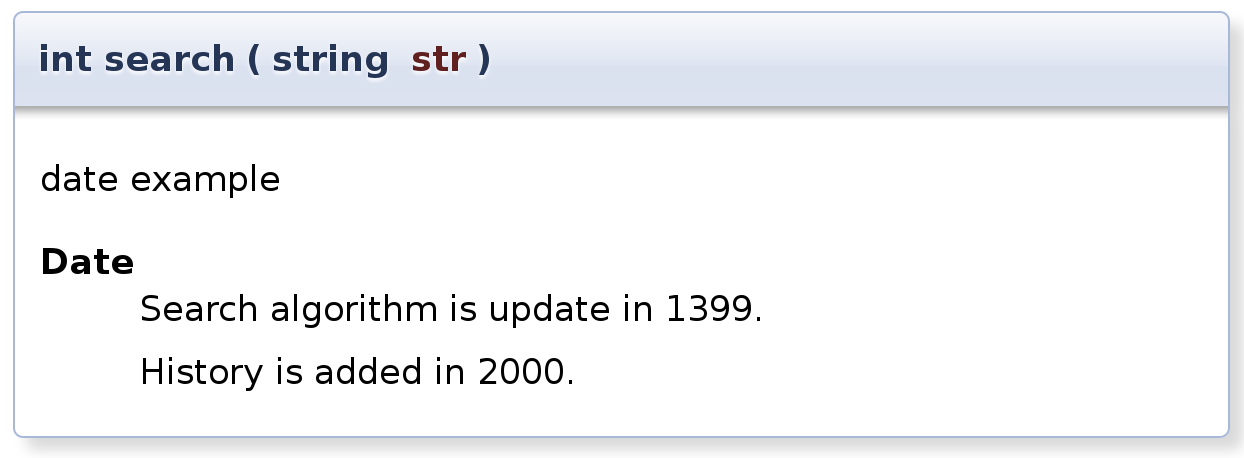
\includegraphics[width=0.8\textwidth]{image/write/document-the-code/developer-info/date-multi}
	\caption[چند برچسب تاریخ]{
		استفاده از چندین برچسب تاریخ پشت سر هم.
	}
	\label{write/document-the-code/developer-info/date-multi}
\end{figure}


\subsection{نسخه}
% version 
% \version { version number }

در پروژه‌های نرم‌افزاری، تغییراتی ایجاد شده در هر بسته با استفاده از یک شماره
مرز بندی می‌شود که به آن نسخه می‌گویند.
برای نمونه فرض کنید که در طول زمان چهار ویژگی به یک بسته نرم‌افزاری اضافه شده
است، یک مرزبندی این است که دو ویژگی در نسخه شماره ۱ و دو ویژگی دگر در نسخه شماره
۲ قرار گیرد.
در نسخه بندی یک سیستم، ترتیب صعودی میان نسخه‌ها به منزله پیشرفت پروژه در نظر
گرفته می‌شود.
در نمونه اورده شده نیز بعد از نسخه شماره ۲ تمام چهار ویژگی در سیستم وجود خواهد
داشت در حالی که نسخه شماره ۱ تنها شامل دو ویژگی است.
نسخه بندی یک سیستم و یا محصول بر اساس سیاست‌هایی است که در توسعه به کار می‌رود و
در حوزه این کتاب جای ندارد از این رو به آن نخواهیم پرداخت.

مستند فنی، به عنوان یک مستند جامع از یک سیستم باید شامل اطلاعاتی در زمینه نسخه
بندی و ویژگی‌های هر نسخه نیز باشد.
بر این اساس برچسب \lr{version} برای تشریح خصوصیت‌های یک نسخه در مستند فنی در نظر
گرفته شده است.
ساختار کلی این برچسب به صورت زیر است:
\begin{C++}
/**
 * \version { version number }
 */
\end{C++}

متن ورودی این برچسب می‌تواند به صورت یک پاراگراف کامل در نظر گرفته شود که شامل
توضیحات کامل در مورد این نسخه است.
در این متن می‌توان از تمام روش‌های زیباسازی متن و برچسب‌های نمایشی استفاده کرد.
پایان متن ورودی این برچسب با رسیدن به یک خط خالی و یا برچسب تعیین می‌شود.

\begin{note}
این برچسب برای تشریح امکانات، تغییرات و یا به روز رسانی‌هایی استفاده می‌شود و
می‌تواند برای هر موجودیت به صورت جداگانه به کار گرفته شود.
بهتر است از این برچسب زمانی استفاده شود که موجودیت مورد نظر شامل تغییرات و یا
شرایط جدید باشد.
\end{note}

امکان استفاده از این برچسب به صورت متوالی نیز فراهم شده است.
تمام برچسب‌هایی که به صورت متوالی آورده شده باشد، با یک دیگر ترکیب شده و در
خروجی نمایشد داده می‌شود.
توضیحات مربوط به هر نسخه در این حالت با شروع یک خط جدید در مستند نمایش داده شده
و یک خروجی مناسب را ایجاد می‌کند.
یک روش معادل نیز تشریح تمام تغییرات با استفاده از یک برچسب است که استفاده از این
روش توصیه نمی‌شود.


\subsection{نویسندگان}
% author
% \author { list of authors }
% \authors { list of authors }

نام نویسنده و یا نویسندگان، از دیگر اطلاعات توسعه است که در مستند فنی در نظر
گرفته می‌شود.
نام نویسنده و یا نویسندگان را با استفاده از برچسب \lr{author} تعیین می‌کنند که
در حالت کلی به صورت زیر است:
\begin{C++}
/**
 * \author {list of autohrs}
 */
\end{C++}

برای نمونه فرض کنید که یک تابع توسط سه نویسنده پیاده‌سازی شده است، در این صورت
مستند مربوط به این تابع، در حالت کلی، به صورت زیر خواهد بود:
\begin{C++}
/**
 * \brief author example
 *
 * \author author1
 * author2
 * author3
 */
int author(string str);
\end{C++}

مستند نهایی تولید شده برای این مستند در شکل
\ref{write/document-the-code/developer-info/author-multi} نمایش داده شده است.
فهرست نویسندگان، همانگونه در این نمونه قابل ملاحضه است، می‌تواند شامل چندین نام
باشد.
پاراگرافی که بعد از این برچسب نوشته شود به صورت کامل به عنوان پارامتر این برچسب
در نظر گرفته می‌شود.
این برچسب ساختار خاصی را برای پاراگراف ورودی در نظر نمی‌گیرد بنابر این می‌توان
از تمام برچسب‌های که در نمایش متن و زیبا سازی آن کاربرد دارد، استفاده کرد.
انتهای این برچسب با استفاده از یک خط خالی و یا آغاز یک بخش دیگر تعیین می‌شود.
\begin{figure}
	\centering
	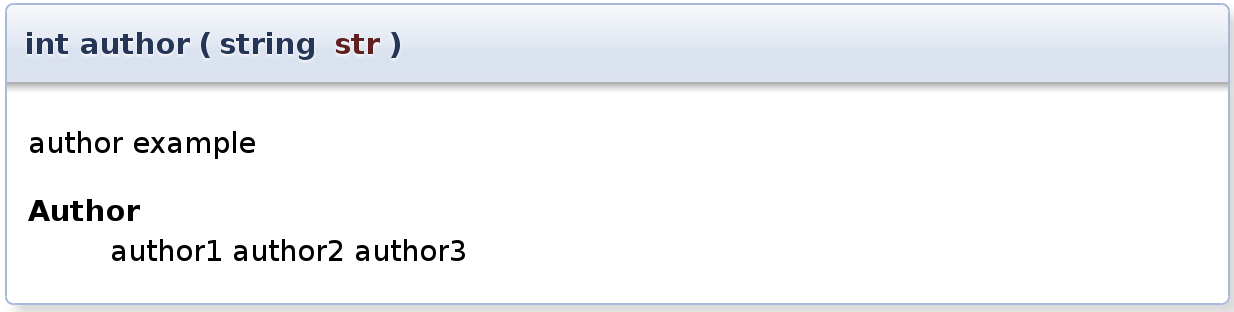
\includegraphics[width=0.8\textwidth]{image/write/document-the-code/developer-info/author-multi}
	\caption[فهرست نویسندگان]{
		فهرست نویسندگان.
	}
	\label{write/document-the-code/developer-info/author-multi}
\end{figure}


همانگونه که در نمونه بالا قابل مشاهده است، می‌توان فهرست تمام نویسندگان را با
استفاده از یک برچسب بیان کرد.
روش مناسب‌تر استفاده از این برچسب برای هر نویسنده است به این ترتیب نام
نویستنده‌گان هرکدام به صورت مستقل در یک خط نوشته می‌شود.
از این رو می‌توان نمونه بالا را به صورت زیر اصلاح کرد:
\begin{C++}
/**
 * \brief author example
 *
 * \author author1
 * \author author2
 * \author author3
 */
int author1(string str);
\end{C++}
مستند تولید شده برای این مستند در شکل \ref{write/document-the-code/developer-info/author-multi1}
نمایش داده شده است.
\begin{figure}
	\centering
	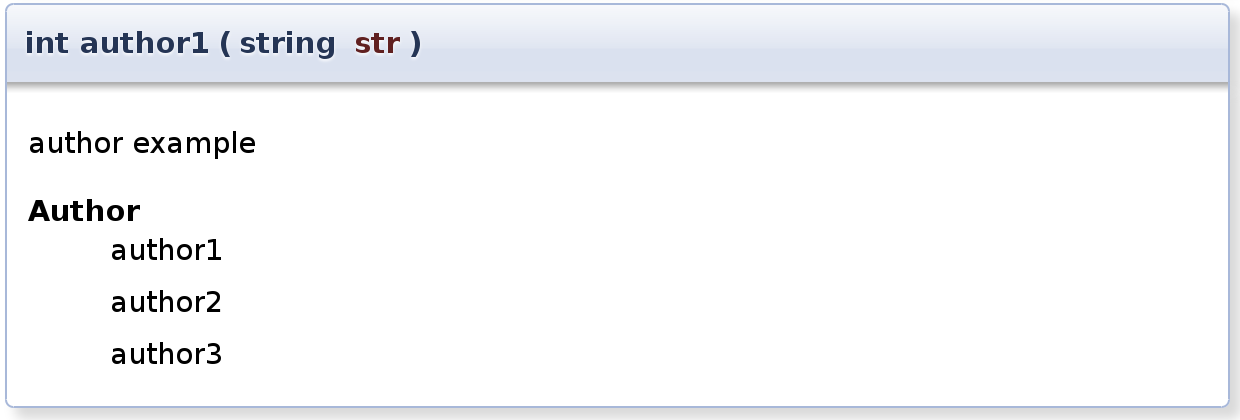
\includegraphics[width=0.8\textwidth]{image/write/document-the-code/developer-info/author-multi1}
	\caption[فهرست نویسندگان]{
		فهرست نویسندگان با به کاربردن چندین برچسب متوالی.
	}
	\label{write/document-the-code/developer-info/author-multi1}
\end{figure}

یک روش دیگر استفاده از برچسب \lr{authors} است.
تنها تفاوت میان این دو برچسب، عنوانی است که در خروجی تولید می‌شود.
با استفاده از برچسب \lr{authors} عنوان تولید شده در خروجی نیز به صورت جمع خواهد
بود در حالی که برچسب \lr{author} به صورت مفرد است.
به عنوان نمونه اصلاح نمونه بالا به صورت زیر مستند شکل
\ref{write/document-the-code/developer-info/author-multi2} را ایجاد می‌کند که
تنها در عنوان با یکدیگر متفاوت هستند.
\begin{C++}
/**
 * \brief author example
 *
 * \authors author1
 * \authors author2
 * \authors author3
 */
int authors(string str);
\end{C++}
\begin{figure}
	\centering
	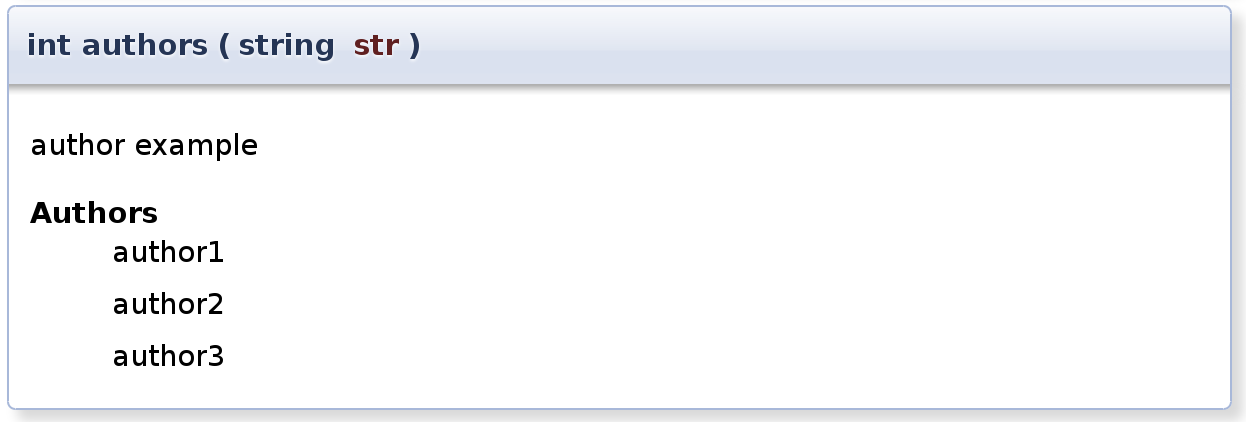
\includegraphics[width=0.8\textwidth]{image/write/document-the-code/developer-info/author-multi2}
	\caption[فهرست نویسندگان]{
		فهرست نویسندگان با استفاده از برچسب \lr{authors}.
	}
	\label{write/document-the-code/developer-info/author-multi2}
\end{figure}


\subsection{نسخه شروع}
% since
% \since { text }

در فرآیند توسعه سیستم‌ها، موجودیت‌های و امکانات متفاوت در برهه‌های زمانی و یا
نسخه‌های متفاوتی از سیستم ایجاد می‌شوند.
با استفاده از برچسب \lr{since} زمان اضافه شدن یک موجودیت به بسته اضافه تعیین می‌شود.
ساختار کلی این برچسب به صورت زیر است:
\begin{C++}
/**
 * \since { text }
 */
\end{C++}

در متن ورودی این برچسب، که در حالت کلی یک پاراگراف است، از ساختار خاصی استفاده نمی‌شود
و می‌توان تمام برچسب‌های زیباسازی متن را در آن به کار برد.
متن ورودی این برچسب با رسیدن به یک سطر خالی و یا برچسب‌های دیگر خاتمه می‌یابد.
برای نمونه فرض کنید که یک فراخوانی از نسخه ۲ یک بسته معرفی شده است، مستند مورد نیاز برای 
این فراخوانی، در ساده‌ترین حالت، به صورت زیر است:
\begin{C++}
/**
 * \brief since example
 *
 * \since 2.0.0 last update
 */
int since(string str);
\end{C++}

مستند ایجاد شده برای این نمونه در شکل \ref{write/document-the-code/developer-info/since} نمایش 
داده شده است.
\begin{figure}
	\centering
	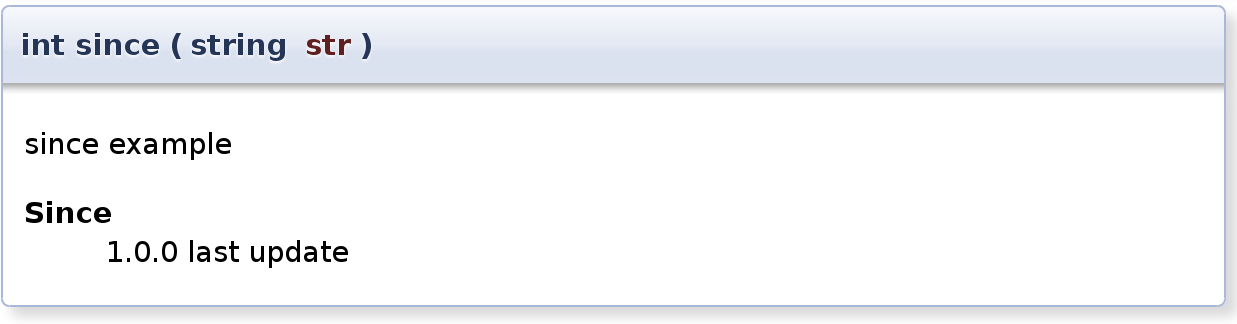
\includegraphics[width=0.8\textwidth]{write/document-the-code/developer-info/since}
	\caption[فهرست نویسندگان]{
		تعیین رویداد و یا نسخه‌ای اضافه شدن یک سیستم.
	}
	\label{write/document-the-code/developer-info/since}
\end{figure}

\begin{warning}
امکان استفاده از این برچسب بیش از یک بار برای هر موجودیت وجود دارد با این وجود این کار
از نظر مستند سازی کاملا اشتباه است.
ظهور یک امکان جدید تنها در یک زمان ممکن است و بعد از آن ممکن است دستخوش تغییراتی شده
و به روز شود.
برای نمایش تغییرات و به روز رسانی‌های از برچسب‌های دیگری مانند \lr{date}
\end{warning}

\subsection{کنارگذاشتن}
% deprecated
% \deprecated { description }

کنار گذاشتن و یا حذف یک امکان از سیستم در طول حیات آن بسیار معمول است.
در بسیاری از موارد امکانات ایجاد شده کارایی خود را از دست داده و یا با امکانات
جدید اضافه شده در تضاد هستند.
از این رو باید به ناچار آنها را کنار گذاشت و این موضوع را به نوعی به کاربران آن
سیستم انتقال داد.
اما سیستم‌ها باید به گونه‌ای توسعه یابند که با سازکارهای قدیم خود سازگار بوده و
سیستم‌های وابسته به خود را حمایت کنند.
نمی‌توان اینگونه تصور کرد که به محض کنار گذاشتن یک امکان از طراحی، در پیاده سازی
نیز باید آن را حذف کرد.

یک روش مناسب برای کنار گذاشتن یک امکان از سیستم، اعلام این کار در نسخه جاری و
اجرای آن در نسخه‌های آینده است.
در این روش امکان مورد نظر به صورت یک امکان کنار گذاشته معرفی می‌شود و در مستند
فنی به کاربران سیستم اعلام می‌شود.
در نهایت بعد از چند نسخه، بنا بر سیاست‌های توسعه، امکان مورد نظر به صورت کامل
حذف می‌شود.
در مستند سازی فنی از برچسب \lr{depricated} برای تعیین امکاناتی استفاده می‌شود که
در حال حاضر کنار گذاشته شده و در آینده نیز به صورت کامل از سیستم حذف می‌شود.
ساختار کلی این برچسب به صورت زیر است:
\begin{C++}
/**
 * \deprecated {description }
 */
\end{C++} 

از این برچسب برای تشریح ورش‌های جایگزین، زمان انقضا و حذف کامل و یا هر مستند
مورد نیاز برای موجودیت و یا امکان کنارگذاشته شده، استفاده می‌شود.
برای نمونه فرض کنید که یک فراخوانی در سیستم در نظر گرفته شده بوده است و در
طراحی به این نتیجه رسیده‌ایم که این فراخوانی باید حذف شود.
حداقل مستند مورد نیاز برای این فراخوانی به صورت زیر است:
\begin{C++}
/**
 * \brief deprecated example
 *
 * \deprecated This method will be removed in V2.0.1 completely, please use
 * deprecated2(string) instead.
 */
int deprecated(string str);
\end{C++}

در شکل \ref{write/document-the-code/developer-info/deprecated} خروجی تولید شده
برای این مستند نمایش داده شده است.
در فرآیند تولید مستند فنی، تمام موجودیت‌هایی که به عنوان یک موجودیت کنارگذاشته
شده تعیین می‌شوند در یک فهرست جمع آورده شده و به مستند اضافه می‌شود.
به این ترتیب با ارائه شدن یک نسخه جدید از سیستم و مستند فنی آن، کاربران
می‌توانند به سادگی فهرست تمام امکانات کنارگذاشته شده را مشاهده و تغییرهای مورد
نیاز را در سیستم‌های خود ایجاد کنند.
در شکل \ref{write/document-the-code/developer-info/deprecated-list} یک نمونه از
فهرست موجودیت‌های کنارگذاشده شده آورده شده است.
\begin{figure}
	\centering
	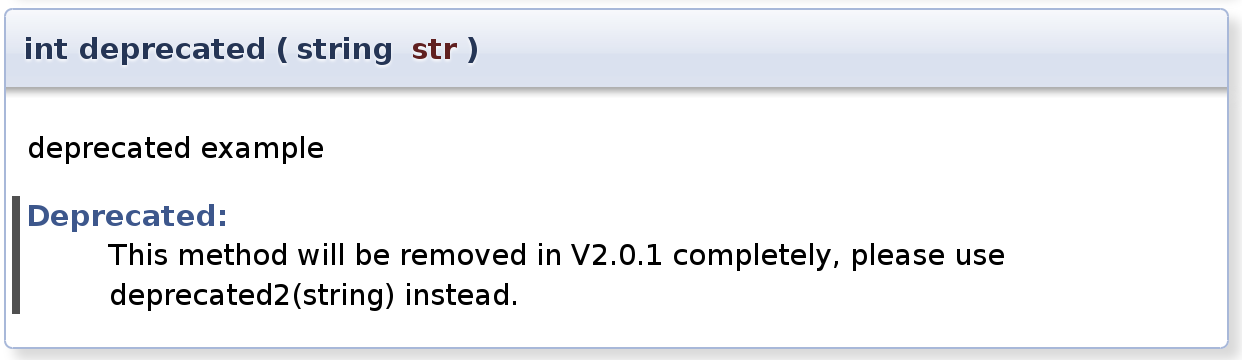
\includegraphics[width=0.8\textwidth]{image/write/document-the-code/developer-info/deprecated}
	\caption[موجودیت کنار گذاشته شده]{
		مستند یک موجودیت کنار گذاشته شده. در این مستند نه تنها روش جایگزین بلکه زمان
		حذف کامل این موجودیت نیز بیان شده است.
	}
	\label{write/document-the-code/developer-info/deprecated}
\end{figure}
\begin{figure}
	\centering
	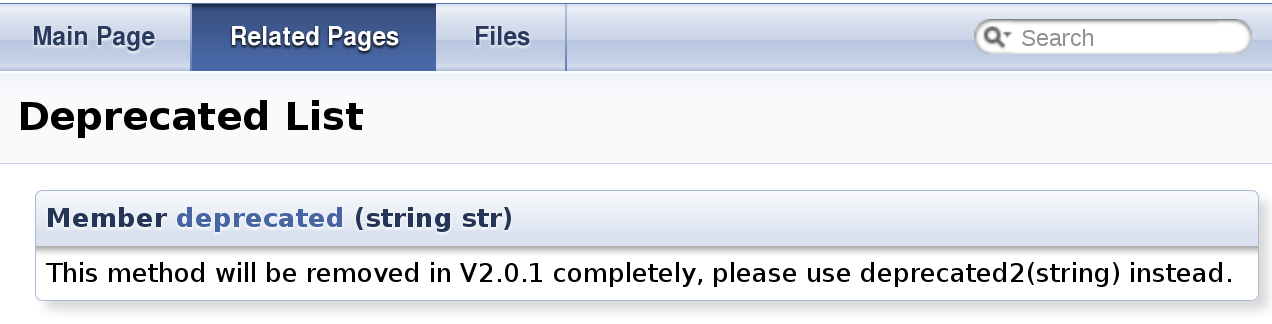
\includegraphics[width=0.8\textwidth]{write/document-the-code/developer-info/deprecated-list}
	\caption[فهرست موجودیت‌های کنار گذاشته شده]{
		فهرست تمام موجودیت‌های حذف شده. این فهرست کاربران را در توسعه و تغییر سیستم‌های خود
		یاری می‌کند.
	}
	\label{write/document-the-code/developer-info/deprecated-list}
\end{figure}


% \subsection{بخش}
% remarker
% \remark { remark text }
% 
% Starts a paragraph where one or more remarks may be entered. The paragraph will
% be indented. The text of the paragraph has no special internal structure. All
% visual enhancement commands may be used inside the paragraph. Multiple adjacent
% \remark commands will be joined into a single paragraph. Each remark will start
% on a new line. Alternatively, one \remark command may mention several remarks.
% The \remark command ends when a blank line or some other sectioning command is
% encountered.




\section{مستند توابع}

تابع‌ها یکی از پایه‌ای ترین موجودیت‌ها در زبان‌های برنامه سازی هستند.
پیدایش تابع مصادف با ارائه شدن راهکارهای برنامه سازی به صورت پیمانه‌ای بوده است.
امروزه تقریبا تمام زبان‌های برنامه‌سازی عمومی مبتنی بر توابع طراحی و پیاده سازی
می‌شوند.
در مستند نویسی نیز نگاهی ویژه به این موجودیت وجود دارد.
در مستند فنی برچسب‌ها و راهکارهای متفاوتی برای مستند سازی این موجودیت ارائه شده
است که در این بخش به بررسی این موارد خواهیم پرداخت.

\subsection{پارامترها}
% param
% \param [(dir)] <parameter-name> { parameter description }

پارامترهای ورودی و خروجی مهم‌ترین خصوصیت از یک تابع است که در مستند فنی باید به آن پرداخته شود.
برای توصیف پارامترها تابع برچسب \lr{param} در نظر گرفته شده است.
مستند فنی پارامترها انقدر مهم است که در فرآیند تولید مستند فنی، پارامترهای بدون مستند کشف شده و 
به صورت اخطار نمایش داده می شود.
ساختار کلی این برچسب به صورت زیر است:
\begin{C++}
\param [(dir)] <parameter-name> { parameter description }
\end{C++}

اولین پارامتر این برچسب جهت پارامتر را برای تابع تعیین می‌کند.
اگر پارامتر یک پارامتر ورودی برای تابع باشد با \lr{in} و اگر پارامتر
به عنوان خروجی تابع در نظر گرفته شده باشد با \lr{out} نمایش داده می‌شود.
برای پارامترهایی که در یک تابع به عنوان ورودی و خروجی به کار می‌روند، هر دو مقدار 
با هم به کار می‌رود.
در نمونه زیر هر سه حالت ممکن برای جهت پارامترها وجود دارد. 
\begin{C++}
/**
 * \brief Function argument example
 *
 * \param[in]      param1 First argument.
 * \param[out]      param2 Second argument.
 * \param[in,out] param3 Third argument.
 */
int param(string param1, int* param2, double* param3);
\end{C++}

پارامتر دوم نام پارامتر و پاراگراف بعد از آن توصیف پارامتر است. در شکل
\ref{write/document-the-code/function/param} مستند تولید شده برای نمونه
بالا آورده شده است.
\begin{figure}
	\centering
	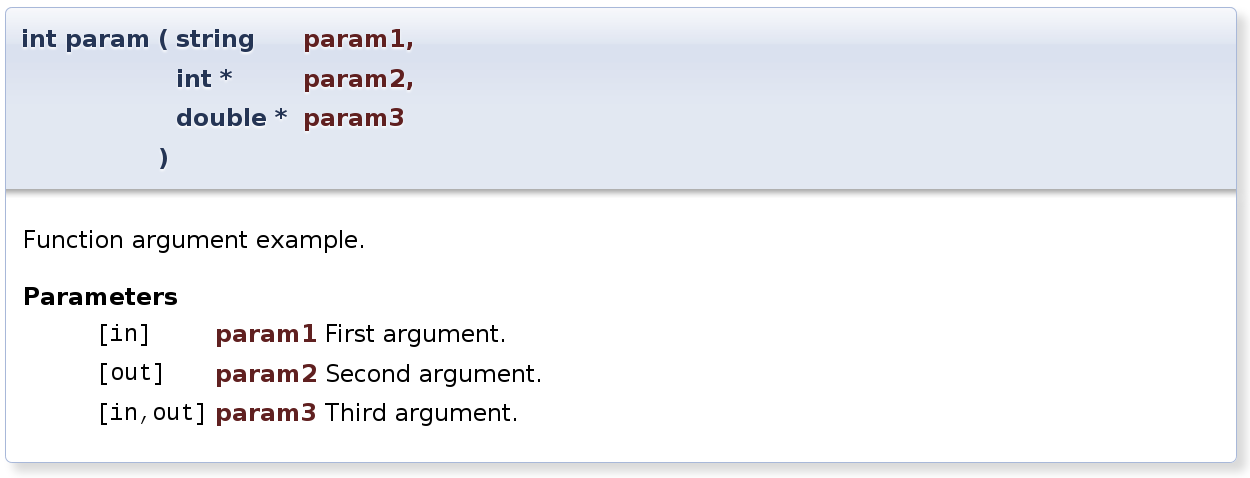
\includegraphics[width=0.8\textwidth]{write/document-the-code/function/param}
	\caption[پارامترهای یک تابع]{
		پارامترهای یک تابع.
	}
	\label{write/document-the-code/function/param}
\end{figure}

توصیف پارامتر ورودی از ساختار خاصی پیروی نمی‌کند و می‌تواند شامل تمام دستورهای
زیبا سازی متن باشد.
تمام برچسب‌های \lr{param} که پست سر هم قرار می‌گیرند با هم ادغام شده و به صورت یک 
بخش مستقل در مستند ظاهر می‌شوند.
در این بخش مستند توصیف هر پارامتر از یک خط جدید آغاز می‌شود.
شروع یک برچسب و یا بخش دیگر انتهای توصیف این برچسب را تعیین می‌کند.

در بسیاری از موارد چندین پارامتر برای نمایش یک موجودیت به کار گرفته می‌شوند.
برای نمونه یک نقطه در فضای سه بعدی با استفاده از سه عدد نمایش داده می‌شود.
در این حالت می‌توان نام چندین پارامتر را به صورت هم زمان به عنوان ورودی نام 
برای این برچسب به کار برد.
نام پارامترها در این حالت با استفاده از کاما از یکدیگر جدا می‌شود.
در زیر یک نمونه آورده شده است که در آن سه پارامتر با هم مستند شده است.
مستند تولید شده برای این نمونه نیز در شکل 
\ref{write/document-the-code/function/param-multi-with-single-tag} نمایش داده شده است.
\begin{C++}
/**
 * \brief Multiple parameter with single param tag.
 * \param x,y,z Coordinates of the position in 3D space.
 * \param t     Time of event.
 */
void param2(double x,double y,double z,double t);
\end{C++}

\begin{figure}
	\centering
	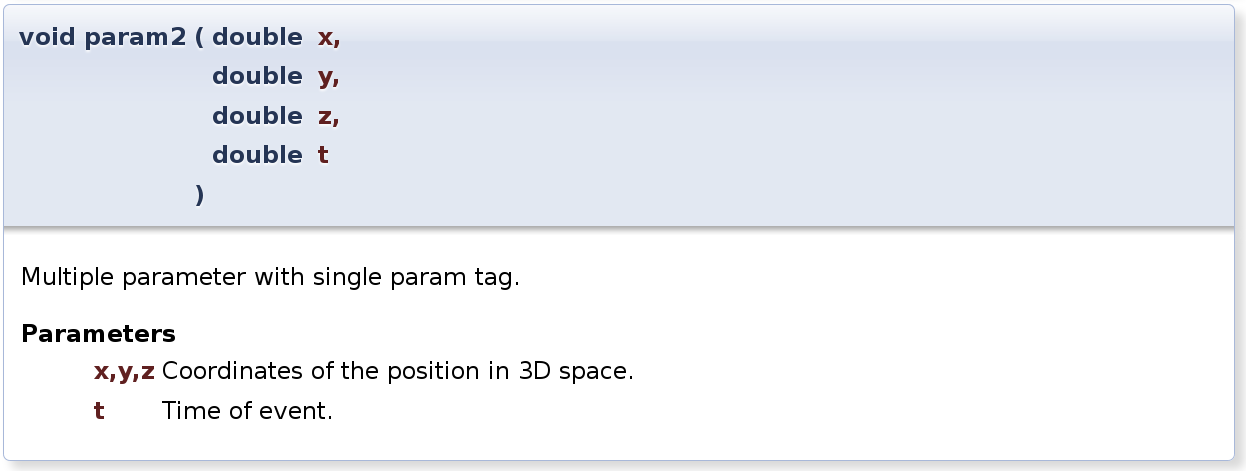
\includegraphics[width=0.8\textwidth]{write/document-the-code/function/param-multi-with-single-tag}
	\caption[پارامترهای یک تابع]{
		پارامترهای یک تابع. زمانی که چندین پارامتر برای یک کار مشترک به کار گرفته می‌شود
		می‌توان تمام آنها را به صورت یکجا مستند کرد. در این نمونه یک نقطه سه بعدی با سه 
		عدد صحیح نمایش داده شده است و در مستند فنی هر سه با هم مستند شده.
	}
	\label{write/document-the-code/function/param-multi-with-single-tag}
\end{figure}



\subsection{خروجی}
% return
% \return { description of the return value }

در اغلب زبان‌های برنامه سازی همه منظوره، یک نوع داده به عنوان نوع داده خروجی تابع
در نظر گرفته می‌شود.
در مستند سازی فنی برچسب \lr{return} برای مستند کردن خروجی تابع در نظر گرفته شده است.
ساختار کلی استفاده از این برچسب به صورت زیر است:
\begin{C++}
\return { description of the return value }
\end{C++}

ساختار متن توصیف خروجی یک تابع، از ساختار خاصی پیروی نمی‌کند و می‌تواند شامل
انواع برچسب‌های زیبا سازی متن باشد.
بر خلاف اینکه بسیاری از زبانهای مشهور مانند \lr{java}، \lr{C/C++} و \lr{C\#} تنها از 
یک نوع داده خروجی حمایت می‌کنند، امکان استفاده مکرر از این برچسب نیز وجود دارد.
در فرآیند تولید مستند فنی، تمام برچسب‌های \lr{return} که به صورت متوالی ظاهر شده‌اند
با یکدیگر ترکیب شده و در یک بخش نمایش داده می‌شوند.
متن توصیف خروجی تابع با شروع بخش جدید و یا یک برچسب دیگر، پایان می‌یابد.

در \lr{Doxygen} یک برچسب دیگر به نام \lr{returns} برای تشریح خروجی‌های یک تابع در نظر گرفته شده است.
از این برچسب زمانی استفاده می‌شود که بیش از یک خروجی برای یک تابع در نظر گرفته شده است.
ساختار کلی این برچسب به صورت زیر است:
\begin{C++}
\returns { description of the return value }
\end{C++}

\begin{note}
برچسب \lr{returns} کاملا شبیه به \lr{return} است و ویژگی خاصی ندارد. 
زمانی که تعداد خروجی‌های بیش از یکی باشد این برچسب مستند زیباتر و قابل درکی را 
ایجاد می‌کند.
\end{note}

\subsection{استثناها}
% throw
% exception
% \exception <exception-object> { exception description }

با ظهور زبان‌های برنامه سازی، راهکارهایی برای مدیریت خطا پیشنهاد شد که در آن
یک تابع خطا را تولید یک خروجی خاص نمایش می‌داد.
این نوع خروجی را \glspl{exception} می‌نامند که در زبان‌های برنامه سازی راهکاری متفاوت
از خروجی‌های معمولی را برای آنها در نظر می‌گیرند.
نکته‌ای که در مستند سازی فنی باید به آن توجه داشت این است که تمام استثناهای یک
تابع باید به صورت کامل مستند شود.
برای مستند کردن \glspl{exception} از برچسب \lr{exception} استفاده می‌شود.
ساختار کلی این برچسب به صورت زیر است:
\begin{C++}
\exception <exception-object> { exception description }
\end{C++}

دو پارامتر ورودی برای این برچسب در نظر گرفته شده که به ترتیب نام و توصیف استثنا
است.
وجود یک استثنا در یک تابع بررسی نمی‌شود از این رو مستند ساز باید در
مستند کردن استثنا دقت کند.
پاراگراف توصیف استثنا از ساختار خاصی پیروی نمی‌کند و می‌توان از برچسب‌های دیگر مانند
برچسب‌های زیبا سازی متن در آن استفاده کرد.
متن توصیف یک استثنا با رسیدن به یک خط خالی، بخش جدید و یا برچسب دیگر پایان می‌پذیرد.

معمولا توابع انواع متفاوتی استثنا تولید می‌کنند که هر یک حالت خاصی را نمایش می‌دهد.
از این رو امکان استفاده از چندین برچسب \lr{exception} فراهم شده است.
در فرآیند تولید مستند فنی، برچسب‌هایی که به صورت متوالی ظاهر شده‌اند با هم ترکیب
شده و در یک بخش نمایش داده می‌شوند.
در این حالت توصیف هر استثنا با شروع یک خط جدید آغاز می‌شود.
در نمونه زیر تابعی با دو نوع استثنا متفاوت مستند شده است و خروجی معادل با آن در شکل 
\ref{write/document-the-code/function/exception} نمایش داده شده است.
\begin{C++}
/**
 * \brief exception explanation
 *
 * \exception Exp1 Exception should be discussed here.
 * \exception Exp2 Exception should be discussed here.
 * \exception Exp3 Exception should be discussed here.
 *
 * This section causes new exception section to be generated by Doxygen.
 *
 * \exception Exp4 Exception should be discussed here.
 * \exception Exp5 Exception should be discussed here.
 */
int excetpion(Param p1, Param p2);
\end{C++} 
\begin{figure}
	\centering
	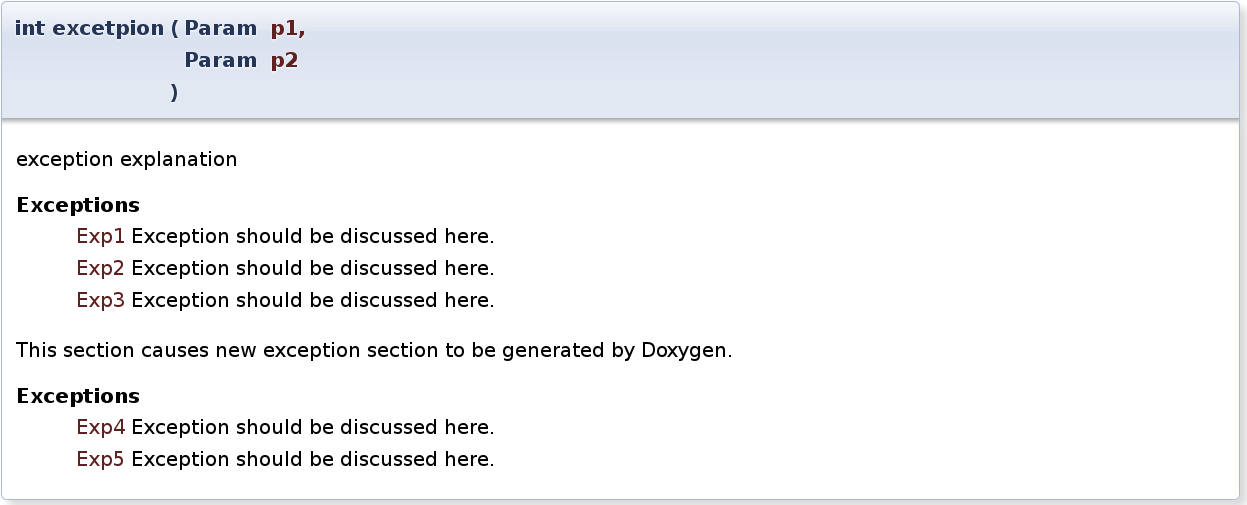
\includegraphics[width=0.8\textwidth]{image/write/document-the-code/function/exception}
	\caption[استثناهای یک تابع]{
		برچسب‌های \lr{exception} که به صورت پشت سر هم اورده شده است با یک دیگر ترکیب شده 
		و در یک بخش نمایش داده می‌شود.
	}
	\label{write/document-the-code/function/exception}
\end{figure}

برخی از ابزارهای مستند سازی از برچسب \lr{throw} برای توصیف یک استثنا استفاده می‌شود.
شاید دلیل این کار کلمه ذخیره شده \lr{throw} است که برای تولید یک استثنا در برخی
از زبان‌های برنامه سازی مانند \lr{C++} و \lr{java} استفاده می‌شود.
در \lr{Doxygen} نیز از این برچسب حمایت می‌شود.
ساختار کلی این برچسب به صورت زیر است:
\begin{C++}
\throw <exception-object> { exception description }
\end{C++}

زمانی که تعداد استثناها بیش از یکی باشد، می‌توان از برچسب \lr{throws} نیز استفاده کرد.

% TODO: maso 1392: پیش نیاز و پس نیاز یک تابع
% \subsection{پیش نیاز و پس نیاز}
% \post { description of the postcondition }
% 
% Starts a paragraph where the postcondition of an entity can be described. The
% paragraph will be indented. The text of the paragraph has no special internal
% structure. All visual enhancement commands may be used inside the paragraph.
% Multiple adjacent \post commands will be joined into a single paragraph. Each
% postcondition will start on a new line. Alternatively, one \post command may
% mention several postconditions. The \post command ends when a blank line or some
% other sectioning command is encountered.
% 
% \pre { description of the precondition }
% 
% Starts a paragraph where the precondition of an entity can be described. The
% paragraph will be indented. The text of the paragraph has no special internal
% structure. All visual enhancement commands may be used inside the paragraph.
% Multiple adjacent \pre commands will be joined into a single paragraph. Each
% precondition will start on a new line. Alternatively, one \pre command may
% mention several preconditions. The \pre command ends when a blank line or some
% other sectioning command is encountered.


% TODO: maso 1392: گراف فراخوانی یک تابع
% \subsection{گراف فراخوانی}
% callgraph
% callergraph
% \callgraph
% 
% When this command is put in a comment block of a function or method and HAVE_DOT
% is set to YES, then doxygen will generate a call graph for that function
% (provided the implementation of the function or method calls other documented
% functions). The call graph will be generated regardless of the value of
% CALL_GRAPH.
% 
% Note
%     The completeness (and correctness) of the call graph depends on the doxygen
%     code parser which is not perfect.
% 
% See Also
%     section \callergraph.
% 
% \callergraph
% 
% When this command is put in a comment block of a function or method and HAVE_DOT
% is set to YES, then doxygen will generate a caller graph for that function
% (provided the implementation of the function or method calls other documented
% functions). The caller graph will be generated regardless of the value of
% CALLER_GRAPH.
% 
% Note
%     The completeness (and correctness) of the caller graph depends on the
%     doxygen code parser which is not perfect.
% 
% See Also
%     section \callgraph.









% 
\section{محیط‌های خاص}


note

warning

bug

todo

attention

brief

detail

verbatin

test

code


% %
% حق نشر 1390-1402 دانش پژوهان ققنوس
% حقوق این اثر محفوظ است.
% 
% استفاده مجدد از متن و یا نتایج این اثر در هر شکل غیر قانونی است مگر اینکه متن حق
% نشر بالا در ابتدای تمامی مستندهای و یا برنامه‌های به دست آمده از این اثر
% بازنویسی شود. این کار باید برای تمامی مستندها، متنهای تبلیغاتی برنامه‌های
% کاربردی و سایر مواردی که از این اثر به دست می‌آید مندرج شده و در قسمت تقدیر از
% صاحب این اثر نام برده شود.
% 
% نام گروه دانش پژوهان ققنوس ممکن است در محصولات دست آمده شده از این اثر درج
% نشود که در این حالت با مطالبی که در بالا اورده شده در تضاد نیست. برای اطلاع
% بیشتر در مورد حق نشر آدرس زیر مراجعه کنید:
% 
% http://dpq.co.ir/licence
%
\section{مدیریت مستندها}

if

copycode

copybrief

copydetail

include

includehtml

htmlonly

xmlonly

latexonly

manonly


% %
% حق نشر 1390-1402 دانش پژوهان ققنوس
% حقوق این اثر محفوظ است.
% 
% استفاده مجدد از متن و یا نتایج این اثر در هر شکل غیر قانونی است مگر اینکه متن حق
% نشر بالا در ابتدای تمامی مستندهای و یا برنامه‌های به دست آمده از این اثر
% بازنویسی شود. این کار باید برای تمامی مستندها، متنهای تبلیغاتی برنامه‌های
% کاربردی و سایر مواردی که از این اثر به دست می‌آید مندرج شده و در قسمت تقدیر از
% صاحب این اثر نام برده شود.
% 
% نام گروه دانش پژوهان ققنوس ممکن است در محصولات دست آمده شده از این اثر درج
% نشود که در این حالت با مطالبی که در بالا اورده شده در تضاد نیست. برای اطلاع
% بیشتر در مورد حق نشر آدرس زیر مراجعه کنید:
% 
% http://dpq.co.ir/licence
%
\section{پیوند}


می‌توان با استفاده از دستورهای متفاوت منابع را بیان کرد. پیوند میان مستندها را
ایجاد کرد. از این میان می‌توان به موارد زیر اشاره کرد:

ref

cite

ancher

see

sa

link



% این مستند در مورد ایجاد فهرست در Doxygen است. 
% مصطفی برمشوری ۱۳۹۰
\chapter{ایجاد فهرست}

\lr{Doxygen} روشهای متفاوتی را برای ایجاد یک فهرست در مستندها فراهم کرده است.
روشهای تعیین شده در \lr{Doxygen} را می توان به سه دسته تقسیم کرد: روشهای داخلی،
استفاده از برچسبهای \lr{HTM} و استفاده از برچسبهای تعریف شده در دیگر ابزارهای
مستند سازی . گرچه روشهای داخلی تعریف شده در \lr{Doxygen} روش مناسبی را برای
ایجاد فهرست فراهم کرده‌اند اما استفاده از برچسبهای \lr{HTML} برتریهایی نسبت به
این روشها دارد که در ادامه به آنها خواهیم پرداخت.

از آنجا که یکی از هدف‌های \lr{Doxygen} توانایی تولید مستند بر اساس دیگر
استاندارهای مستند سازی است، برچسبهای مورد استفاده در دیگر ابزارهای مستند سازی
نیز به صورت داخلی تعریف شده و قابل استفاده می باشد. از این رو نه تنها می‌توان از
روش‌های ایجاد شده در دیگر ابزارها استفاد کرد بلکه مستند‌های ایجاد شده مبتنی بر
استانداردهای دیگر را نیز مورد استفاده قرار داد.

\section{روش داخلی}

در این روش هر گزینه از فهرست با استفاده از یک خط تیره (علامت منفی) در ابتدای سطر
تعیین می‌شود. زمانی که نیاز به ایجاد یک گزینه شماره دار باشد بعد از خط تیره
علامت عدد (?) نیز قرار می‌گیرد. برای ایجاد زیر فهرست برای یک گزینه باید گزینه
های جدید را با استفاده از فضای خالی جلوتر از گزینه مورد نظر قرار داد.
در زیر یک نمونه فهرست ایجاد شده به این روش آورده شده است.

\begin{latin}
\lstset{language=C++}  
\begin{lstlisting}[frame=single] 
/**
 *  A list of events:
 *    - mouse events
 *         -# mouse move event
 *         -# mouse click event\n
 *            More info about the click event.
 *         -# mouse double click event
 *    - keyboard events
 *         -# key down event
 *         -# key up event
 *
 *  More text here.
 */
\end{lstlisting}
\end{latin}

در نهایت زمانی که با استفاده از \lr{Doxygen} این مستند به قالبهای دیگر تبدیل شود
نتیجه‌ای مشابه به نوشته زیر به دست خواهد آمد.

 \begin{latin}
    \begin{itemize}
	\item mouse events
		\begin{itemize}
			\item  mouse move event
			\item  mouse click event
			\item   More info about the click event.
			\item   mouse double click event
		\end{itemize}
	\item keyboard events
		\begin{itemize}
			\item  key down event
			\item  key up event
		\end{itemize}
  \end{itemize}
\end{latin}

\begin{note}
 تعیین  سطح جدید از فهرست نیاز به ایجاد فضای خالی به اندازه یک \lr{TAB} در
 ابتدای هر گزینه دارد اما ممکن است که اندازه \lr{TAB} در هر مستند متفاوت باشد.
 از این رو پیش از هر چیز از این نکته اطمینان حاصل کنید که به چه اندازه باید فضای
 خالی استفاده شود. میزان فضای خالی مورد استفاده برای هر \lr{TAB} در پرونده
 تنظیمات موجود است. این اندازه به صورت پیشفرض برابر با هشت فضای خالی در نظر
 گرفته می شود.
\end{note}

برای تعیین انتهای یک فهرست (در هر سطح) به دو روش می توان عمل کرد. در روش نخست یک
سطر خالی بعد از گزینه نوشته می‌شود. این روش زمانی مناسب است که یک فهرست به صورت
کامل تمام شده است و بعد از آن متنهای دیگری از مستند قرار خواهد گرفت. در روش دوم
در یک سطر جدید یک نقطه گذاشته می شود.
این روش برای نشان دادن انتهای فهرستی که دارای چندین سطح می‌باشند مناسب است. در
نمونه زیر  چگونگی استفاده از نقطه برای تعیین انتهای یک فهرست نشان داده شده است.

\begin{latin}
\lstset{language=C++}  
\begin{lstlisting}[frame=single] 
/**
 * Text before the list
 * - list item 1
 *   - sub item 1
 *     - sub sub item 1
 *     - sub sub item 2
 *     . 
 *     The dot above ends the sub sub item list.
 *     More text for the first sub item
 *   .
 *   The dot above ends the first sub item.
 *   More text for the first list item
 *   - sub item 2
 *   - sub item 3
 * - list item 2
 * .
 * More text in the same paragraph.
 *
 * More text in a new paragraph.
 */
\end{lstlisting}
\end{latin}

\section{برچسب‌های ابر متن}

یک روش ساده و بسیار مناسب برای ایجاد فهرست استفاده از برچسب‌های \lr{HTML} است. 
برتری مهم این روش نسبت به روش‌های دیگر، امکان استفاده از چندین پاراگراف در نوشتن
یک گزینه است.  در زیر نمونه مطرح شده در قسمت پیشین با استفاده از برچسب‌های
\lr{HTML} باز نویسی شده است.

\begin{latin}
\lstset{language=C++}  
\begin{lstlisting}[frame=single] 
  /*! 
   *  A list of events:
   *  <ul>
   *  <li> mouse events
   *     <ol>
   *     <li>mouse move event
   *     <li>mouse click event\n
   *         More info about the click event.
   *     <li>mouse double click event
   *     </ol>
   *  <li> keyboard events
   *     <ol>     
   *     <li>key down event
   *     <li>key up event
   *     </ol>
   *  </ul>
   *  More text here.
   */
\end{lstlisting}
\end{latin}

از انجا که فهرست‌هایی که در سطح‌های پایین‌تر قرار می‌گیرند با استفاده از برچسب
نشان داده می‌شود دیگر نیازی به استفاده از فضای خالی در ابتدایی یک گزینه نیست.
شاید بتوان این خصوصیت را یک برتری نسبت به روش پیشین در نظر گرفت.

\section{برچسب‌های دیگر ابزارها}

همانگونه که پیش از این بیان شده، برای ایجاد توانایی حمایت از مستندهای تولید شده
بر اساس دیگر استانداردها، دسته ای از برچسب‌ها به استاندارد \lr{Doxygen} اضافه
شده است. برای نمونه می‌توان به برچسب‌های \lr{arg} و \lr{li} اشاره کرد. این
برچسب‌ها در ابزارهای مستند سازی مانند \lr{QtDoc} و \lr{KDoc} مورد استفاده قرار
می‌گیرد.

بنابر این می‌توان از روش‌های معادل در ابزارهای دیگر فهرست‌های دلخاه را ایجاد
کرد. البته ایجاد این توانایی با اشکال‌هایی هم روبرو شده است که در ادامه به صورت
جداگانه به آنها پرداخته خواهد شد.

\subsection{\lr{QtDoc}}

هر فهرست در مستندهای \lr{QtDoc} با استفاده از برچسب \lr{list} و \lr{endlist}
ایجاد می‌شود. در حالت کلی یک فهرست به صورت زیر است:

\begin{latin}
\lstset{language=C++}  
\begin{lstlisting}[frame=single] 
/*! 
 * \list
 *	<list items>
 * \endlist
 */
\end{lstlisting}
\end{latin}

که در آن \lr{<list items>} می‌تواند یک گزینه و یا حتی یک فهرست دیگر باشد. بدهی
است که ایجاد فهرست‌های تودرتو با استفاده از این برچسب‌ها در \lr{QtDoc} ممکن
خواهد بود.

در این ابزار از برچسب \lr{li} برای ایجاد یک گزینه استفاده می‌شود. از این برچسب
نه تنها در ایجاد گزینه‌ها در یک فهرست بلکه برای ایجاد سطر در جدول نیز مورد
استفاده قرار می‌گیرد. در اینجا تنها کاربرد این برچسب در ایجاد یک فهرست مد نظر
خواهد بود.
در حالت کلی ایجاد یک گزینه در فهرست با استفاده از این برچسب به صورت زیر است:

\begin{latin}
 \lstset{language=C++}  
\begin{lstlisting}[frame=single] 
/*! 
 *  \li {item description}
 */
\end{lstlisting}
\end{latin}

پارامتر ورودی یک توصیف از گزینه مورد نظر است. متن هر گزینه با رسیدن به یکی از
موارد زیر پایان خواهد یافت:
\begin{itemize}
  \item یک سطر خالی
  \item بر چسب دیگری از \lr{li}
  \item برچسب پایان یک فهرست یا \lr{list}
  \item برچسب آغاز یک فهرست یا \lr{endlist}
\end{itemize}

\begin{warning}
گرچه می‌توان با استفاده از برچسب‌هایی مانند \lr{list} و \lr{endlist} فهرست‌های
تودرتو ایجاد کرد اما در \lr{Doxygen} این برچسب‌ها مورد حمایت قرار نگرفته است.
تنها برچسب مورد حمایت در این ابزار \lr{li} است. از این رو فهرست‌های ایجاد شده با
روش‌های معرفی شده در \lr{QtDoc} به صورت یک فهرست ساده و تک سطحی، در خروجی‌های
\lr{Doxygen} ظاهر خواهد شد.
\end{warning}

برای نمونه در مستند زیر یک فهرست ایجاد شده است که خرجی مشابه‌ای در \lr{Doxygen}
و \lr{QtDoc} دارد.

\begin{latin}
 \lstset{language=C++}  
\begin{lstlisting}[frame=single] 
/**
 * \list
 *  \li \c AlignLeft left alignment.
 *  \li \c AlignCenter center alignment.
 *  \li \c AlignRight right alignment
 *	  No other types of alignment are supported.
 * \endlist
 */
\end{lstlisting}
\end{latin}

\subsection{\lr{KDoc}}

این ابزار که معادل با ابزار \lr{JavaDoc} است، برای ایجاد مستند فنی بر اساس
برنامه‌های نوشته شده به زبان برنامه نویسی جاوا مورد استفاده قرار می‌گیرد. در این
ابزار با استفاده از برچسب \lr{arg} یک فهرست ایجاد می‌شود. این برچسب دارای تنها
یک پارامتر ورودی است. ساختار کلی این برچسب به صورت زیر است.

\begin{latin}
\lstset{language=C++}  
\begin{lstlisting}[frame=single] 
  /*! 
   *  \arg {item description}
   */
\end{lstlisting}
\end{latin}

پارامتر ورودی در حقیقت متنی است که گزینه را توصیف می‌کند. متن هر گزینه با قرار
دادن یک سطر خالی و یا شروع شدن یک برچسب جدید \lr{arg}  پایان می‌پذیرد. به این
نکته باید توجه کرد که با استفاده از این برچسب نمی‌توان فهرست‌های چند سطحی را
ایجاد کرد.

\begin{latin}
 \lstset{language=C++}  
\begin{lstlisting}[frame=single] 
/**
 * \arg \c AlignLeft left alignment.
 * \arg \c AlignCenter center alignment.
 * \arg \c AlignRight right alignment
 *	 No other types of alignment are supported.
 * 
 */
\end{lstlisting}
\end{latin}

%
% حق نشر 1390-1402 دانش پژوهان ققنوس
% حقوق این اثر محفوظ است.
% 
% استفاده مجدد از متن و یا نتایج این اثر در هر شکل غیر قانونی است مگر اینکه متن حق
% نشر بالا در ابتدای تمامی مستندهای و یا برنامه‌های به دست آمده از این اثر
% بازنویسی شود. این کار باید برای تمامی مستندها، متنهای تبلیغاتی برنامه‌های
% کاربردی و سایر مواردی که از این اثر به دست می‌آید مندرج شده و در قسمت تقدیر از
% صاحب این اثر نام برده شود.
% 
% نام گروه دانش پژوهان ققنوس ممکن است در محصولات دست آمده شده از این اثر درج
% نشود که در این حالت با مطالبی که در بالا اورده شده در تضاد نیست. برای اطلاع
% بیشتر در مورد حق نشر آدرس زیر مراجعه کنید:
% 
% http://dpq.co.ir/licence
%
% در این قسمت به بررسی تمام روش های مورد استفاده در Doxygen خواهیم پرداخت که در
% دسته بندی مستندها مورد استفاده قرار می گیرد.
% مصطفی برمشوری ۱۳۸۹/۲ این یک گفتار است نه یک قسمت. باید این را اصلاح کرد.

\chapter{بخش بندی}

\lr{Doxygen} از سه روی کرد برای بخش بندی کردن مستندها حمایت می کند:
پیمانه‌ها، برگه‌ها و دسته‌بندی اعضا.
 یک دسته گردایه‌ای از مستندها است که میان آنها از نظر منطقی، یک ارتباط خاص وجود
 دارد. علاوه بر مستندهایی که یک دسته را تشکیل می‌دهند، همواره یک صفحه مستند در
 نظر گرفته می‌شود که در آن به خود دسته به صورت اختصاصی توصیف می‌شود.
 با استفاده از برگه‌ها امکان تعریف یک مستند با موضوعی خاص در مستندهای تکنیکی
 فراهم شده است. برای نمونه تشریح معماری‌های مورد حمایت سیستم، که به طور مستقیم
 به هیچ یک از قسمتهای مستند وابسته نیست، می‌تواند در یک برگه توصیف شد. در
 \lr{Doxygen} امکانهای متفاوتی برای مدیریت برگه‌ها تعریف شده است که با استفاده
 از آنها می‌توان یک مستند کاملا ساختارمند را ایجاد کرد.
 
 تمام اجزای سیستم و مستند‌های ایجاد شده برای آنها بر اساس قراردادهایی از پیش
 تعریف شده مرتب می‌شود. برای نمونه تمام متغیرهایی که در یک کلاس تعریف می‌شود بر
 اساس نام مرتب شده و در یک دست جای خواهد گرفت. اما روش‌ها و قراردادهایی از پیش
 تعریف شده همواره روش‌های مناسبی نمی‌تواند در نظر گرفته شود. از این رو باید
 روش‌هایی تعریف شود که بتوان خارج از این قراردادهای مستندهای ایجاد شده را دسته
 بندی کرد. مستندگر \lr{Doxygen} امکانهای مناسبی را برای مدیریت و دسته بندی اجزا
 فراهم کرده است که می‌تواند در سازماندهی کردن مستندهای ایجاد شده مورد استفاده
 قرار گیرد.
 
روش‌های متفاوت معرفی شده در \lr{Doxygen} برای دسته بندی کردن مستند‌ها، امکان
سازماندهی و مدیریت مستندهایی با حجم بسیار بالا را فراهم کرده است. با استفاده از
این روش‌های می‌توان به سادگی دسته بندی مستندها را ایجاد کرده و فرآیند توسعه
مستند تکنیکی سیستم را بهبود بخشید. در این گفتار هر یک از رویکردهای مورد استفاده
در \lr{Doxygen} را به صورت کامل مورد بررسی قرار خواهیم داد.




\section{برگه‌ها}

یک برگه عبارت است از یک مستند کاملا سازماندهی شده که به صورت مستقیم با هیچ یک از
موجودیت‌های یک سیستم در ارتباط نیست. به بیان دیگر یک برگه گرچه به عنوان قسمتی از
مستند فنی در نظر گرفته می شود اما به صورت مستقیم هیچ یک از موجودیت‌های سیستم
مانند کلاسها، فضاهای نام و غیره را تشریح نمی‌کند.

مستندهای که مانند مستند نصب و راه اندازی یک سیستم، که به صورت مستقیم مربوط به
قسمتی خاص از یک سیستم نمی‌شود ولی در عین حال یک مستند فنی بسیار مهم در نظر گرفته
می‌شود، با استفاده از برگه‌ها ایجاد می‌شوند.

گرچه در فرآیند مستند فنی، در ساختارهای متفاوت، دید متفاوتی نسبت به یک برگه وجود
دارد اما در حالت کلی می‌توان یک برگه را معادل با یک گفتار در نظر گرفته که به
توصیف و تشریح جنبه‌ای خاص از سیستم می‌پردازد. در حالت کلی یک برگه به صورت زیر در
مستند فنی ایجاد می‌شود:


\begin{latin}
\lstset{language=C++}  
\begin{lstlisting}[frame=single] 
\page <name> (title)
\end{lstlisting}
\end{latin}

که در آن \lr{<name>} یک شناسه و \lr{(title)} عنوان مورد نظر برای برگه است. عنوان
یک عبارت است که برای نمایش یک برگه به کار می‌رود در حالی که شناسه تنها برای
ایجاد پیوند به هر برگه مورد استفاده قرار می‌گیرد. برخلاف عنوان که می‌تواند هر
عبارتی باشد شناسه تنها از حروف نوشتاری و عدد ایجاد می‌شود که شامل هیچ فاصله‌ای
نیست.

\begin{note}
شناسه ترکیبی از حروف و ارقام است. در برخی از سیستم‌های عامل مانند لینوکس و
یونیکس، حروف بزرگ و کوچک با یکدیگر تفاوت دارند در حالی که در برخی دیگر اینگونه
نیست. از این رو ممکن است برخی از توسعه دهندگان از حروف بزرگ و یا ترکیب آن با
حروف کوچک برای ایجاد شناسه استفاده کنند (برای نمونه \lr{MyPage01}). 
\\%FIXME: maso 1391 این قسمت باید به دو پاراگراف تبدیل شود.
گرچه استفاده از حروف بزرگ و کوچک در نامگذاری برگه‌ها مخصوصا زمانی که اندازه
مستند بزرگ است، می‌تواند مفید باشد اما با مشکل‌های نیز روبرو است. برای نمونه در
ایجاد مستند فنی نهای بر اساس قالب خاص، مانند \lr{HTML} پرونده‌هایی هم نام با
شناسه‌های برگه‌ها ایجاد می‌شود از این رو در سیستم عامل‌هایی مانند ویندوز، که در
آنها تفاوتی میان حروف بزرگ و کوچک نیست، مشکلهایی در خروجی ایجاد شده به وجود
می‌اید. از این رو بهتر است که تمام شناسه‌ها را تنها با استفاده از حروف کوچک
ایجاد کرد.
\end{note}

برای نمونه قطعه مستند زیر را در نظر بگیرید:
\begin{latin}
\lstset{language=C++}  
\begin{lstlisting}[frame=single] 
/**
 * \page pageinstall Install
 * 
 * Installation (or setup) of a computer program (including device drivers and plugins),
 * is the act of making the program ready for execution. Because the process varies
 * for each program and each computer, programs (including operating systems) often
 * come with an installer, a specialized program responsible for doing whatever is
 * needed for their installation.
 */
\end{lstlisting}
\end{latin}

در این نمونه یک برگه با عنوان \lr{Install} ایجاد شده است که با استفاده از شناسه
\lr{pageinstall} شناخته می‌شود. متن هر برگه نیز می‌تواند با استفاده از تمام
برچسب‌های مورد حمایت در \lr{Doxygen} ایجاد شود.


\subsection{بخش بندی برگه}

بخش بندی عبارت از فرآیندی که در آن یک مستند بزرگ به صورت منطقی به صورت تکه‌های
مستند کوتاه در یک ساختار سلسله مراتبی سازماندهی می‌شوند. امروزه بخش بندی کردن
مستندها انقدر مرسوم است که حتی یک مستند چند صفحه‌ای هم بخش بندی می‌شود. برای
نمونه یک کتاب را در نظر بگیرید که در آن موضوع‌های متفاوت با استفاده از فصل‌ها و
گفتارها جدا شده‌اند. با وجود دسته بندی مطالب یک بر اساس موضوع آنها در گفتارهای
متفاوت، خود گفتارها نیز باز به صورت بخش و زیر بخش سازماندهای می‌شوند.

سازماندهی کردن یک مستد بزرگ با استفاده از بخش بندی نه تنها مطالعه و درک آن را
راحتر می‌کند بلکه فرآیند توسعه و نگه داری آن را هم نیز بهبود می‌بخشد. تصور اینکه
یک نویسنده کتابی چند صد صفحه‌ای را بدون تقسیم بندی و سازماندهی کردن بتواند ایجاد
کند انقدر دشوار است که می‌توان آن را معادل با ایجاد یک سیستم بدون معماری در نظر
گرفت. می‌توان گفت بخش بندی در حقیقت ایجاد یک معماری برای یک مستند بزرگ است از
این رو در توسعه و به کار گیری آن بسیار موثر خواهد بود.

از سویی ایجاد یک مستند ساختارمند استفاده از آن را نیز آسان می‌کند. امروزه تمام
کتاب‌ها و مستندها از تکنیک‌های مانند فهرست گذاری استفاده می‌کنند که در آن  یک
فهرست از تمام موضوع‌ها و ارجاع به آن ( مانند شماره صفح) وجود دارد، استفاده
می‌کنند. ایجاد یک فهرست مناسب برای یک مستند بسیار حیاطی است. اما ایجاد این فهرست
به صورت دستی بسیار زمانگیر است و در محیط‌هایی که مستند به سرعت تغییر می‌کند یک
ایراد اساسی به شمار می‌آید. با این وجود اگر از تکنیک‌های مناسبی برای ایجاد
بخش‌ها استفاده شود به سادگی می‌توان فهرست‌ها را به صورت خودکار ایجاد کرد و از
هزینه‌های توسعه مستند کاست.

یک مستند را می‌توان به صورت یک درخت در نظر گرفته که به صورت موضوعی ایجاد شده
است. برای نمونه ساختار درختی در شکل 
\ref{images/write/grouping/section-tree} را در نظر بگیرید. در این شکل (که قسمتی
از ساختار سلسله مراتبی این کتاب را نمایش می‌دهد) یک ساختار درختی نمایش داده شده
است که سازمان کلی یک مستند را نمایش می‌دهد. این ساختار از بالاترین سطح با
استفاده از فصل، گفتار، بخش، زیر بخش  و \ldots در یک مستند حقیقی پیاده سازی
می‌شود.

\begin{figure}
	\centering
	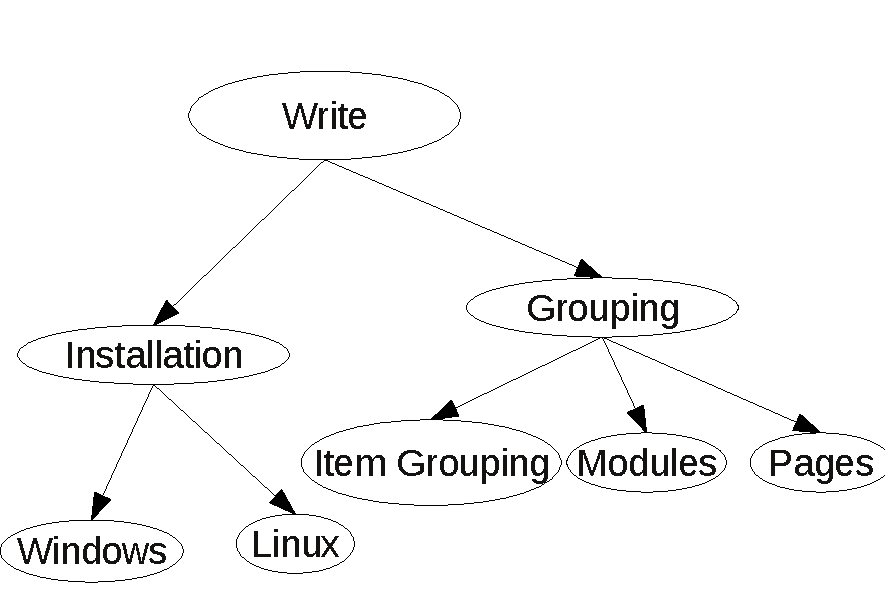
\includegraphics[width=0.75\textwidth]{images/write/grouping/section-tree}
	\caption[ساختار سلسله مراتبی یک مستند]{
		همان گونه که در این شکل نمایش داده شده است یک مستند را می‌توان با استفاده
		از یک ساختار سلسله مراتبی که به صورت یک درخت قابل بیان است، سازماندهی کرد.
	}
	\label{images/write/grouping/section-tree}
\end{figure}

ساختارهای متفاوت نشر، روش‌هایی را برای پیاده سازی این ساختار سلسله مراتبی
پیشنهاد می‌کنند. برای نمونه \lr{HTML} که به عنوان پر کاربرد ترین ساختار متنی در
شبکه جهانی، با استفاده از مفاهیم سرآیندها این ساختار را پیاده سازی می‌کند. در
این ساختار بالاترین سطح یک مستند با استفاده از برچسب \lr{<h1>\ldots</h1>} ایجاد
می‌شود. سطح‌های بعدی مستند که می‌تواند به صورت تود در تو مورد استفاده قرار گیرد
با استفاده از برچسب‌های \lr{<h2>\ldots</h2>}, \ldots و \lr{<h9>\ldots</h9>}
ایجاد می‌شود. از این رو ساختار معرفی شده در
شکل\ref{images/write/grouping/section-tree} به صورت زیر قابل بیان است:

\begin{latin}
\lstset{language=HTML}  
\begin{lstlisting}[frame=single] 
<h1>Writer</h1>
	<h2>Grouping</h2>
		<h3>Pages</h3>
		<h3>Modules</h3>
		<h3>Item Grouping</h3>
	<h2>Installation</h2>
		<h3>Linux</h3>
		<h3>Windows</h3>
\end{lstlisting}
\end{latin}

امکان ایجاد ساختار سلسله مراتبی در مستندهای تکنیکی نیز می‌تواند بسیار مفید باشد
مخصوصا زمانی که مستندهای تکنیکی به مرور زمان و به سرعت تغییر می‌کنند و یا اینکه
اندازه مستندهای ایجاد شده بزرگ باشد. در این بخش برچسب‌های تعریف شده در
استانداردهای \lr{Doxygen} که در ایجاد این ساختار سلسله مراتبی مورد استفاده قرار
می‌گیرد را به صورت کامل مورد بررسی قرار خواهیم داد.

\begin{note}
ساختارهای سلسله مراتبی معرفی شده در این بخش نه تنها قابل استفاده در برگه‌ها
هستند بلکه می‌توان آنها را در هر قسمت دیگر از مستند نیز به کار برد.
\end{note}

% TODO: مصطفی ۱۳۹۱: تعیین منبع برای نوشتن استاندار
% در نوشتن استاندارد از چهار سطح استفاده می‌شود که باید منبع آن را ذکر کرد. فکر
% کنم از استانداردهای ISO برای مستند کاربری بود.
\begin{info}
بر اساس استانداردهای موجود در ایجاد مستندها، ایجاد ساختار سلسله مراتبی در متن
مستند، با بیش از چهار سطح مناسب نیست.  از این رو در بسیاری از ابزارهای مستند
سازی مانند \lr{Doxygen} تنها امکان ایجاد سلسله مراتبی با کمتر از چهار سطح فراهم
شده است.
\end{info}

\paragraph{بخش}

بخش\LTRfootnote{Section} بالاترین سطح را در ساختار سلسله مراتبی مستند دارد.
در حالت کلی یک بخش با استفاده از برچسب \lr{\\Section} و به صورت زیر ایجاد
می‌شود:


\begin{C++}
\section <section-name> (section title)
\end{C++}

این برچسب شامل دو پارامتر است که عبارت اند از \lr{<section-name>} و \lr{Section
title}. نام به صورت یک شناسه در نظر گرفته می‌شود که با استفاده از آن می‌توان یک
بخش را به صورت منحصر به فرد آدرس دهی کرد. این شناسه تنها باید با استفاده از حروف
و ارقام ایجاد شده و شامل هیچ فاصله‌ای نباشد. عنوان یک بخش نیز یک عبارت است که
برای نمایش بخش مورد استفاده قرار می‌گیرد.

\begin{warning}
از این برچسب تنها در یک برگه (یا یک بسته مستند) استفاده می شود و نمی‌تواند در
سطوح پایین تر سلسله مراتبی مستند مورد استفاده قرار گیرد.
\end{warning}
    

\paragraph{زیر بخش}

زیر بخش\LTRfootnote{Subsection} دومین سطح از ساختار سلسله مراتبی مستندهای فنی را
ایجاد می‌کند. این سطح از مستند با استفاده از برچسب \lr{subsection} ایجاد می‌شود
که در حالت کلی به صورت زیر است:

\begin{C++}
\subsection <subsection-name> (subsection title)
\end{C++}

این برچسب نیز شامل دو پارامتر است که عبارت اند از \lr{<subsection-name>} و
\lr{Subsection title}. نام به صورت یک شناسه در نظر گرفته می‌شود که بر اساس قواعد
تعیین شناسه (یعنی تنها با استفاده از حروف و ارقام ایجاد شده و شامل هیچ فاصله‌ای
نباشد) ایجاد شده و با استفاده از آن می‌توان یک زیر بخش را به صورت منحصر به فرد
آدرس دهی کرد.
. عنوان یک زیر بخش نیز یک عبارت است که برای نمایش زیر بخش مورد استفاده قرار
می‌گیرد.

\begin{warning}
یک زیر بخش تنها باید در یک بخش مورد استفاده قرار گیرد و استفاده آن در هر قسمت
دیگر مجاز نمی باشد.
\end{warning}

زیر بخش، در ساختار سلسله مراتبی مستند به عنوان یک قسمت از بخشی در نظر گرفته
می‌شود که پیش از زیر بخش مورد نظر ظاهر شده است. برای نمونه قطعه مستند زیر را در
نظر بگیرید:

\begin{latin}
\lstset{language=C++}  
\begin{lstlisting}[frame=single] 
/**
 * ...
 * \section section1 Writer
 * ...
 * \section section2 Appendex
 * ...
 * \subsection subsection1 Performance
 * ...
 */
\end{lstlisting}
\end{latin}

در این تکه مستند دو بخش و یک زیر بخش ایجاد شده است. زیر بخش ایجاد شده با شناسه
\lr{subsection1} به نزدیکترین بخشی که پیش از آن تعریف شده است تعلق دارد از این
رو این زیر بخش به عنوان یک زیر بخش از بخش \lr{section2} در نظر گرفته می‌شود.

\paragraph{زیر زیر بخش}

سومین سطح در ساختار سلسله مراتبی مستندها را زیر زیر
بخش\LTRfootnote{Subsubsection} ایجاد می‌کند. برای ایجاد یک زیر زیر بخش در مستند
فنی از برچسب \lr{subsubsection} استفاده می‌شود که در حالت کلی به فرم زیر است:

\begin{latin}
\lstset{language=C++}  
\begin{lstlisting}[frame=single] 
\subsubsection <subsubsection-name> (subsubsection title)
\end{lstlisting}
\end{latin}

در اینجا نیز همانند برچسب زیر بخش، از دو پارامتر استفاده می‌شود که عبارت‌اند از:
\lr{subsubsection-name} و \lr{subsubsection-title}. این پارامترها که به ترتیب
شناسه و عنوان زیر زیر بخش را ایجاد می‌کنند، از همان قواعدی که برای زیر بخش بیان
شده است پیروی می‌کنند.

\begin{warning}
شناسه‌هایی که برای یک بخش، زیر بخش , \ldots در نظر گرفته می‌شود باید در حالت کلی
منحصر به فرد باشد. به بیان دیگر زمانی که برای یک بخش از یک شناسه استفاده می شود
نباید شناسه مورد استفاده را برای هیچ بخش، زیر بخش، و غیر به کار برد.
\end{warning}

استفاده از یک زیر زیر بخش تنها در یک زیر بخش مجاز است. هر زیر زیر بخش به عنوان
یک زیر بخش از نزدیکترین زیر بخشی در نظر گرفته می‌شود که پیش از آن تعریف شده
باشد. تکه مستند زیر را در نظر بگیرید:

\begin{latin}
\lstset{language=C++}  
\begin{lstlisting}[frame=single] 
/**
 * ...
 * \section section1 Writer
 * ...
 * \subsection subsection11 Installation
 * ...
 * \subsubsection subsubsection111 Linux
 * \subsubsection subsubsection112 Windows
 * ...
 * \subsection subsection12 Grouping
 * ...
 * \subsubsection subsubsection121 Pages
 * \subsubsection subsubsection122 Modules
 * \subsubsection subsubsection123 Pages
 * ...
 * \section section2 Appendex
 * ...
 * \subsection subsection1 Performance
 * ...
 */
\end{lstlisting}
\end{latin}

در این قطعه مستند سه زیر بخش با شناسه‌های \lr{subsubsection12x} ایجاد شده است.
از آنجا که نزدیکترین زیر بخش تعریف شده قبل از این سه زیر زیر بخش، زیر بخش با
شناسه \lr{subsection12} است، هر سه این زیر زیر بخش ها در این زیر بخش قرار خواهند
گرفت. نمونه بالا معادل با ساختار سلسله مراتبی است که در شکل
\label{write-grouping-pages-section-tree} نمایش داده شده است.
 
    
\paragraph{پاراگراف}

چهارمین سطح از ساختار سلسله مراتبی پاراگراف\LTRfootnote{Paragraph} است که در
حقیقت آخرین سطح از ساختار سلسله مراتبی در نظر گرفته می‌شود. هر تکه متن نوشته شده
در مستند به صورت یک پاراگراف در نظر گرفته می‌شود اما با این حال می‌توان با
استفاده از برچسب \lr{paragraph} یک پاراگراف را نام گذاری کرد. نام گذاری کردن یک
پاراگراف زمانی که نیاز به ارجا به متن آن باشد بسیار مفید است. ایجاد یک پاراگراف
در حالت کلی به صورت زیر است:

\begin{latin}
\lstset{language=C++}  
\begin{lstlisting}[frame=single] 
\paragraph <paragraph-name> (paragraph title)
\end{lstlisting}
\end{latin}

این برچسب نیز مانند برچسب های پیش از دو پارامتر به نام‌های \lr{paragraph-name} و
\lr{paragraph-title} استفاده می‌کند که بر اساس قواعد تعریف شده در برچسب‌های
پیشنین، تعیین می‌شوند. تفاوت اساسی که میان پاراگراف با تمام برچسب‌هایی که پیش از
برای استفاده در ساختارهای سلسله مراتبی بیان شده است، عدم شماره گزاری شدن این
برچسب است. در خروجی ایجاد شده برای یک پاراگراف، عنوان به صورت برجسته در ابتدای
سطر نوشته شده و متن موجود در ادامه آن آورده می‌شود.

\begin{note}
هر پاراگراف به نزدیکترین برچسب تعریف شده قبل از آن تعلق
دارد که در ساختارهای سلسله مراتبی مورد استفاده قرار می‌گیرد. به بیان دیگر این
برچسب به عنوان زیر بخشی از برگه، بخش، زیربخش، و یا زیر زیر بخشی تعلق دارد که پیش
از آن تعریف شده است.
\end{note}
    

\subsection{\lr{mainpage}}

همواره در قالب‌های متفاوت خروجی، از یک برگه به عنوان برگه نخست در مستند استفاده
می‌شود. گرچه برگه نخست نیز همانند دیگر برگه‌ها ایجاد و ویرایش می‌شود اما برخلاف
برگه‌های دیگر با استفاده از برچسب \lr{mainpage} ایجاد می‌شود. ساختار کلی این
دستور به صورت زیر استک

\begin{latin}
\lstset{language=C++}  
\begin{lstlisting}[frame=single] 
\mainpage [(title)]
\end{lstlisting}
\end{latin}

همانگونه که پیش از این نیز اشاره شده، برای ایجاد یک برگه از دو پارامتر استفاده
می‌شد که عبارت بودند از: عنوان و شناسه. برگه نخست تنها برگه‌ای است که تنها یک
پارامتر دارد و آن هم عنوان است. از آنجا که این برگه همواره در کل مستند فنی یکتا
است، یک شناسه پیش فرض به صورت \lr{index} برای آن در نظر گرفته می‌شود بنابر این
برچسب \lr{mainpage} معادل با برچسب زیر است:

\begin{latin}
\lstset{language=C++}  
\begin{lstlisting}[frame=single] 
\page index [(title)]
\end{lstlisting}
\end{latin}

\begin{warning}
از آنجا که شناسه \lr{index} به صورت پیش فرض برای برگه نخست در نظر گرفته شده است،
استفاده از این شناسه برای دیگر برگه‌های یا بخش‌های مستند مجاز نیست و منجر به
بروز مشکل در خروجی تولید شده می شود.
\end{warning}

به عنوان نمونه در مستند زیر برگه نخست مستند ایجاد شده است. همانگونه که در این
نمونه قابل مشاهده است تمام قواعد تعریف شده برای ایجاد یک برگه در اینجا نیز
برقرار است با این تفاوت که این برگه یک برگه خاص بوده و به عنوان نخستین بخش از
مستند در نظر گرفته می‌شود.

\begin{latin}
\lstset{language=C++}  
\begin{lstlisting}[frame=single]
/** 
 * \mainpage My Personal Index Page
 *
 * \section intro_sec Introduction
 *
 * This is the introduction.
 *
 * \section install_sec Installation
 *
 * \subsection step1 Step 1: Opening the box
 *
 * etc...
 */
\end{lstlisting}
\end{latin}

خروجی تولید شده در قالب \lr{HTML} از این برگه به عنوان نخستین صفحه وب استفاده
می‌کند و نام آن را \lr{index.html} در نظر می‌گیرد در حالی که در قالب \lr{LaTex}
از این برگه به عنوان نخستین گفتار در مستند تولید شده استفاده می‌کند.

\subsection{سازماندهی برگه‌ها}

همان گونه که پیش از این بیان شد،  با استفاه از برچسب‌هایی مانند \lr{mainpage} و
یا \lr{page} می‌توان صفحه‌های متفاوتی را در یک مستند ایجاد کرد. در حالت عادی
صفحه‌های ایجاد شده به صورت یک ساختار هموار، به گونه‌ای که تمام صفحه‌ها در یک سطح
قرار می‌گیرند ساختار بندی خواهد شد. قرار گرفتن تمام صفحه‌های ایجاد شده در یک
مستند به صورت ساختار هموار روش مناسبی نیست. بهترین روش ایجاد یک ساختار سلسله
مراتبی برای تمام صفحه‌ها است.

یک روش ایجاد ساختار سلسله مراتبی استفاده از روشی است که در قسمت دسته‌ها به آن
پرداخته شد. یک روش طبیعی و ساده‌تر به جای استفاده از روشهایی دسته بندی، استفاده
از برچسب \lr{subpage} است. این برچسب برای ایجاد ساختار سلسله مراتبی در صفحات
مستند مورد استفاده قرار می‌گیرد. ساختار کلی این برچسب به صورت زیر است.

\begin{latin}
\lstset{language=C++}  
\begin{lstlisting}[frame=single] 
\subpage <name> ["(text)"]
\end{lstlisting}
\end{latin}

که در آن \lr{name} یک شناسه است که به صورت یکتا یک صفحه از مستند را تعیین
می‌کند. \lr{text} یک عنوان است که در نمایش این پیوند مورد استفاده قرار می‌گیرد.
ساختار کلی این برچسب همانند ساختار برچسب \lr{ref} است با این تفاوت که از این
برچسب تنها برای ایجاد رابطه میان صفحه‌ها و ساختار سلسله مراتبی میان آنها استفاده
می‌شود. در زیر یک نمونه از صفحه بندی آروده شده است.
\begin{latin}
\lstset{language=C++}  
\begin{lstlisting}[frame=single] 
/**
 * \mainpage A simple manual
 * Some general info.
  * This manual is divided in the following sections:
  * - \subpage intro
  * - \subpage advanced "Advanced usage"
  */

/** \page intro Introduction
 * This page introduces the user to the topic.
 * Now you can proceed to the \ref advanced "advanced section".
 */

/** \page advanced Advanced Usage
 * This page is for advanced users.
 * Make sure you have first read \ref intro "the introduction".
 */
\end{lstlisting}
\end{latin}

\begin{note}
نمی‌توان یک صفحه را به صورت زیرصفحه در بیش از یک صفحه دیگر  استفاده کرد. ایجاد
دور (چه مستقیم و چه غیر مستقیم) در زیر صفحه‌ها مجاز نمی‌باشد.
\end{note}




\section{\glspl{doxygen:module}‌}

\glspl{doxygen:module} بندی روشی است که با استفاده از آن می‌توان مستندهای متفاوتی را در یک
مستند مشترک گرد آوری کرد. یک پیمانه را می‌توان به صورت یک گردایه از مستندهای مستقل
تصور کرد که به صورت یک پارچه در یک مکان گردآوری شده است. مستند
پروده‌های دیگر، کلاسها، روندها، متغیرها، تعریف‌ها و یا حتی دسته‌های دیگر  می‌توانند به عنوان
بخشی از یک \glspl{doxygen:module} باشند.
 
توانایی اضافه کردن یک \glspl{doxygen:module}، در \glspl{doxygen:module}‌ای دیگر قابلیت ایجاد ساختار سلسله مراتبی در
دسته‌بندی را فراهم می‌کند. ساختار سلسله مراتبی نه تنها مدیریت مستندهای بزرگ
را ممکن می‌سازد بلکه مستند را در دسترس‌تر خواهد کرد به گونه‌ای که کاربران
می‌توانند به سادگی به مستندهای مورد نیاز خود دست یابند. این دسته بندی می‌تواند بر اساس خواص
مشترک ایجاد شود اما به طور معمول این دسته‌بندی محتوایی است و تمام مستندهای مرتبط را باهم 
دسته بندی کرده و در یک ساختار سلسله مراتبی سازماندهی می‌کند.

\subsection{ایجاد \glspl{doxygen:module}}

برای تعریف یک \glspl{doxygen:module} از برچسب \lr{defgroup} استفاده می شود. با قرار دادن این برچسب
در یک بسته مخصوص (بسته‌های مخصوص را ببینید) یک دسته ایجاد خواهد شده. قالب کلی
استفاده از این برچسب به صورت زیر است:
\begin{C++}
/**
 * \defgroup <name> (group title)
 */
\end{C++}

نخستین \glspl{argument} این برچسب، یک شناسه را برای گروه تعیین می‌کند که باید در تمام
مستند به صورت یکتا تعریف شده باشد. این شناسه (همانند تمام شناسه‌های دیگر) می‌بایست
تنها از یک واژه تشکیل شده باشد. \glspl{argument} دوم عنوان برای دسته
تعیین می‌کند، که در مستندها برای نمایش دسته مورد استفاده قرار می گیرد. 
به عنوان نمونه، کد زیر یک دسته به نام \lr{Example}  را ایجاد می‌کند:

\begin{C++}
/*
 * \defgroup example_group Example
 * This is example group
 */
\end{C++}

مستند مربوط به هر دسته درست بعد از تعریف آن قرار نوشته می‌شود که یک شرح کامل از
آن خواهد بود. این مستند می‌تواند
شامل بخش بندی خاص بوده و از تمام امکانات موجود در مستند سازی بهره ببرد.

\subsection{اضافه کردن به دسته}
اضافه کردن مستند به یک دسته خواص با استفاده از برچسب \lr{ingroup} انجام می‌شود. با
استفاده از این برچسب می‌توان به سادگی یک کلاس، پرونده، متغیر، و یا غیره را به یک یا چند
دسته خواص اضافه کرد. ساختار کلی این برچسب به صورت زیر است.

\begin{C++}
\ingroup (<groupname> [<groupname><groupname>])
\end{C++}
تنها نوع \glspl{argument} در این برچسب، شناسه \glspl{doxygen:module}‌ای است که مستند به آن 
تعلق دارد.

\begin{warning}
امکان اضافه کردن یک مستند به چندین دسته، در نسخه‌های نخستین این بسته فراهم نبوده، از
این رو همواره تلاش کنید که مستندها را به گونه‌ای دسته بندی کنید که هر بخش در یک \glspl{doxygen:module}
قرار گیرد.
\end{warning}

گرچه با استفاده از این برچسب می‌توان یک مستند را به هر دسته‌ای اضافه کرد اما در
بسیاری از حالت‌ها استفاده از آن منجر به به زیاد شدن برچسب‌ها و مشکل شدن مستند سازی
در پروژه‌ها خواهد شد. حالتی را فرض کنید که در آن تعداد زیادی متغیر و یا بسته‌های 
مستند کوتاه و پشت سرهم نوشته شده‌اند و هدف قراردادن تمام این بسته‌های مستند در یک
\glspl{doxygen:module} خاص است. با استفاده از این برچسب باید به ناچار هرکدام از بسته‌ها را به صورت
جداگانه برچسب‌گذاری کرد. 

زمانی که مستند‌ها همگی در یک پرونده و به صورت پشت سرهم ایجاد شده باشند، می‌توان با
استفاده از برچسب \lr{ \ \{  \ \}} به صورت فیزیکی مستند‌ها را در یک گروه قرار داد.
این روش نه تنها در ایجاد دسته‌های و گروه‌ها بلکه در بسیاری از موارد دیگر
مورد استفاده قرار می‌گیرد. راهکار اصلی در این روش استفاده از یک برچسب شروع و پایان
برای تمام اضای یک پیمانه است. در زیر یک نمونه استفاده از این عبارت آمده است.

\begin{C++}
/**
 * \defgroup gexample Example
 * \{
 */
 ...
/**\}*/
\end{C++}
به بیان دیگر برچسب  \lr{ \ \{  \ \}} یک محدوده ایجاد می‌کند که تمام مستندهای تعریف شده در آن
در \glspl{doxygen:module} متناظر با آن محدوده قرار می‌گیرد. اما نکته‌ای که باید در نظر داشت این است که
در اینجا تعریف یک \glspl{doxygen:module} و اضافه کردن مستندها با هم انجام می‌شود.

این روش را می‌توان در ایجاد \glspl{doxygen:module}‌های تودرتو نیز به کاربرد. تنها کافی است که دسته
جدید در محدوده یک دسته دیگر تعریف شود، به این ترتیب دسته دوم به عنوان یک زیر
دسته از دسته اول در نظر گرفته خواهد شد.

زمانی که از یک شناسه مشترک برای تعریف دو دسته استفاده شود، در فرآیند ایجاد
مستند خطا صادر خواهد شده و در بسیاری از موارد این فرآیند با مشکل اساسی روبرو
می‌شود (به بیان دیگر استفاده از یک شناسه برای تعریف دو دسته
مجزا، مجاز نمی باشد). یک روش جایگزین برای تعریف دسته استفاده از برچسب
\lr{addtogroup} است. قالب کلی این برچسب مانند برچسب تعریف یک گروه است. تعریف کلی
این برچسب به صورت زیر است.
\begin{C++}
\addtogroup <name> [(title)]
\end{C++}

یک تفاوت مهم این برچسب با برچسب تعریف دسته  اختیاری بودن عنوان برای \glspl{doxygen:module}
در این برچسب است. اگر یک \glspl{doxygen:module} با یک شناسه تعریف شده باشد، استفاده از این 
دستور برای ایجاد و اضافه کردن یک بسته مستند به گروه مورد نظر با خطا روبرو نخواهد شد.
ام زمانی که هیچ \glspl{doxygen:module}‌ای شناسه مورد نظر یافت نشود، یک \glspl{doxygen:module} ایجاد شده 
و مستندهای مورد نظر به آن اضافه می‌شود. از این رو می‌توان گفت که این تکنیک فرایند تولید
مستند را انعطاف پذیر خواهد کرد.

همان گونه که پیش از این اشاره شده، با ستفاده از برچسب‌های \lr{ \ \{ \ \}} یک محدوده
و مستندهای مورد نظر در آن تعریف می‌شود. تمام مستد‌های تعریف شده در این محدوده به \glspl{doxygen:module} 
مربوط به آن اضافه خواهد شد. این روش را نیز می‌توان با برچسب \lr{addtogroup} به کار برد.
با استفاده از این روش می‌توان مستندها را به صورت فیزیکی دسته بندی کرده و آنها را در
هر گروه دلخواه قرار داد (در تکه مستند زیر استفاده از این روش نشان داده شده است).

\begin{C++}
/**
 * \addtogroup gexample
 * \{
 */
...
/**
 * \}
 */
\end{C++}

با استفاده از برچسب \lr{ref} می‌توان یک پیونده به یک \glspl{doxygen:module} ایجاد کرد. این برچسب که در بخش‌های
بعد مورد بررسی قرار می‌گیرد از یک \glspl{parameter} به عنوان شناسه استفاده می‌کند که مستند مورد نظر
کاربر را تعیین می‌کند. از این برچسب برای ایجاد پیوند به یک \glspl{doxygen:module} نیز استفاده می شود
که \glspl{parameter} ورودی آن شناسه \glspl{doxygen:module} است.

\begin{note}
همواره باید این نکته را به یاد داشت که موجودیت‌های مانند پروند، کلاس ویا فضای
نام را می‌توان در دسته‌های متفاوتی قرار داد در حالی که موجودیت‌های مانند
متغیر، و متد را نمی‌تواند به بیش از یک دسته اضافه کرد. دلیل اصلی این کار پیش‌گیری از
مبهم شدن مستندها است.

با این فرض زمانی که یک موجودیت (به صورت غیرمجاز) به دو یا چند دسته اضافه شود، چه
روی خواهد داد؟ تمام برچسب‌هایی که یک مستند را در یک دسته جای می‌دهند دارای یک
اولویت هستند، از این رو مستند به دسته ای اضافه می‌شود که با استفاده از برچسب با
اولیت بیشتر تعیین شده است. اولویت میان برچسب‌ها عبارت اند از: \lr{ingroup}
\lr{defgroup} \lr{addtogroup} \lr{weakgroup} .
برچسب \lr{weakgroup} همانند برچسب \lr{addtogroup} است با این تفاوت که اولویت آن
نسبت به \lr{addtogroup} کمتر است.

\end{note}



\section{دسته بندی اعضا}

هرگاه یک موجودیت، که خود شامل مستندهای متفاوتی است (برای نمونه یک کلاس را فرض
کنید که شامل روندها، و متغیرهای متفاوت با مستندهای متفاوت است)، پسندیده است که
مستندهای موجود در این موجودیت به صورت مناسب دسته بندی شده باشد. گرچه
\lr{Doxygen} به صورت خودکار اعضای موجود در یک موجودیت را  بر اساس نوع، سطح
دسترسی  و تریب واژکها دسته بندی می‌کند، اما در بسیاری از موارد این گونه
دسته‌بندی‌ها از نظر منطقی کافی نیست. برای نمونه حالتی را تصور کنید که در آن
دسته‌ای از روندها از نظر منطقی با هم در ارتباط هستند، گرچه سطح دسترسی آنها
متفاوت است،  اما قرار داده آنها در یک دسته می‌تواند بسیار مفید باشد. دسته بندی
کردن اعضای یک موجودیت با استفاده از عبارت‌های زیر انجام می‌شود.
\begin{latin}
\lstset{language=C++}  
\begin{lstlisting}[frame=single] 
  /**\{*/
  ...
  /**\}*/
  
  //\{
    ..
  //\}
\end{lstlisting}
\end{latin}

توجه به این نکته ضروری است که، تمام اعضای یک دسته باید به صورت فیزیکی در آن دسته
قرار گیرد. همواره این نیاز  به تعیین یک نام  و توصیف برای یک دسته، در مستند سازی
وجود دارد. برای تعیین کردن نام برای یک دسته از اعضا از برچسب \lr{name} استفاده
می‌شود. ساختار کلی این دستور به صورت زیر است.

\begin{latin}
\lstset{language=C++}  
\begin{lstlisting}[frame=single] 
    /**
     * \name [(header)]
     */
\end{lstlisting}
\end{latin}

که در آن سرایند، نامی است که در مستند تولید شده برای دسته به نمایش در خواهد آمد.
همان گونه که مشخص است تعیین سرایند برای یک دسته از اعضا اختیاری است. مستند مربوط
به دسته بعد از این برچسب نوشته می‌شود به عبارتی، استفاده از این برچسب در یک بسته
مستند به این معنی است که مستند در رابطه با یک دسته از اعضا نوشته شده است.
استفاده از عبارت \lr{ \\{ \\}} بعد از این برچسب اجباری است.

\begin{note}
دسته بندی کردن اعضا به صورت تو در تو مجاز نیست. به بیان دیگر اعضا تنها می‌توانند
در یک سطح دسته بندی شوند.
\end{note}

همواره دسته بندی شدن اعضای یک موجودیت (به ویژه زمانی که این دسته بندی به صورت
خودکار انجام می‌شود) مفید نیست. از این رو برخلاف آنچه که در بالا به آن اشاره شد،
گاهی نیاز است که از دسته بندی شده اعضا جلوگیری کرد. برای نمونه حالتی را تصور
کنید که در آن فهرستی از متغیرهای ایستای عمومی\lr{Public Static} تعریف شده است که
به عنوان کلید و یا مقادیر اولیه در سیستم استفاده می‌شود، اما نوع این متغیرها
متفاوت است. از انجا که نوع این متغیرها متفاوت است \lr{Doxygen} به صورت خودکار
انها را بر اساس نوع در دسته‌های متفاوت قرار خواهد داد. برای جلوگیری کردن از این
حالت از برچسب \lr{nogrouping} استفاده می‌شود. ساختار کلی این دستور به صورت زیر
است.

\begin{latin}
\lstset{language=C++}  
\begin{lstlisting}[frame=single] 
    /**
     * \nogrouping
     */
\end{lstlisting}
\end{latin}

با قرار دادن این برچسب از دسته بندی شدن مستندها به صورت خودکار جلوگیری خواهد شد.
برای روشن شدن چگونگی دسته بندی کردن اعضای یک موجودیت به نمونه زیر توجه کنید.

\begin{latin}
\lstset{language=C++}  
\begin{lstlisting}[frame=single] 
    /** A class. Details */
    class Test{
      public:
	//\{
	/** Same documentation for both members. Details */
	void func1InGroup1();
	void func2InGroup1();
	//\}

	/** Function without group. Details. */
	void ungroupedFunction();
	void func1InGroup2();
      protected:
	void func2InGroup2();
    };
    void Test::func1InGroup1() {}
    void Test::func2InGroup1() {}
    /** \name Group2
    *  Description of group 2. 
    */
    //\{
    /** Function 2 in group 2. Details. */
    void Test::func2InGroup2() {}
    /** Function 1 in group 2. Details. */
    void Test::func1InGroup2() {}
    //\}

    /*! \file 
    *  docs for this file
    */

    //\{
    //! one description for all members of this group 
    //! (because DISTRIBUTE_GROUP_DOC is YES in the config file)
    #define A 1
    #define B 2
    void glob_func();
    //\}
\end{lstlisting}
\end{latin}
در این نمونه \lr{Group1} به عنوان یک زیردسته از \lr{Public Group} تعریف شده است. دسته  \lr{Group2}
به عنوان یک دسته جدا در نظر گرفته خواهد شد، در حالی که روندهای موجود در آن سطح دسترسی متفاوتی را دارند.


%
% حق نشر 1390-1402 دانش پژوهان ققنوس
% حقوق این اثر محفوظ است.
% 
% استفاده مجدد از متن و یا نتایج این اثر در هر شکل غیر قانونی است مگر اینکه متن حق
% نشر بالا در ابتدای تمامی مستندهای و یا برنامه‌های به دست آمده از این اثر
% بازنویسی شود. این کار باید برای تمامی مستندها، متنهای تبلیغاتی برنامه‌های
% کاربردی و سایر مواردی که از این اثر به دست می‌آید مندرج شده و در قسمت تقدیر از
% صاحب این اثر نام برده شود.
% 
% نام گروه دانش پژوهان ققنوس ممکن است در محصولات دست آمده شده از این اثر درج
% نشود که در این حالت با مطالبی که در بالا اورده شده در تضاد نیست. برای اطلاع
% بیشتر در مورد حق نشر آدرس زیر مراجعه کنید:
% 
% http://dpq.co.ir/licence
%
\chapter{فرمول‌نویسی}

در مستندات مختلف ممکن است نیاز داشته باشید فرمول‌هایی بنویسید. این وضعیت در
مستندات فنی یا حتی کاربری مربوط به کتابخانه‌های کاربردی بسیار رایج است. فرض کنید
در حال توسعه یک کتابخانه ریاضی هستید و در مستنداتی که برای این کتابخانه
می‌نویسید نیاز به درج روابط و فرمول‌های ریاضی دارید. سوالی که پیش می‌آید این است
که ابزار \lr{Doxygen} چگونه از فرمول‌نویسی پشتیبانی می‌کند؟ به عبارتی چگونه
می‌توان فرمولی را (مثلا در توضیحات یک کلاس یا متد) نوشت تا در مستندات تولید شده
با استفاده از \lr{Doxygen} نیز این فرمول ظاهر شود.
یکی از امکانات مناسب \lr{Doxygen}، این است که برای نوشتن فرمول می‌توان از قوانین
فرمول‌نویسی \lr{\LaTeX} استفاده کرد. در واقع \lr{Doxygen} فرمول‌نویسی بر اساس قوانین
\lr{\LaTeX} را تشخیص می‌دهد و این سبک فرمول‌نویسی را پشتیبانی می‌کند.
با استفاده از این قابلیت می‌توان رابطه‌های بسیار پیچیده ریاضی را در مستندات
نوشت. لازم به ذکر است که استفاده از فرمول‌های \lr{\LaTeX} تنها برای قالب‌های خروجی
ابرمتن (\lr{HTML}) و \lr{\LaTeX} امکان‌پذیر است و برای خروجی‌های در قالب \lr{RTF} و
\lr{man page} کار نمی‌کند.

در این فصل ابتدا توضیح داده می‌شود که فرمول‌هایی که به سبک \lr{\LaTeX} نوشته می‌شوند
در قالب‌های خروجی مختلف چگونه ظاهر می‌شوند و چه ابزاری برای استفاده از این
امکانات نیاز است. سپس فرمول‌نویسی به سبک \lr{\LaTeX} به صورت خلاصه شرح داده می‌شود.
در پایان نیز فرمول‌نویسی مناسب برای \lr{Doxygen} (که بر مبنای قوانین فرمول‌نویسی
\lr{\LaTeX} است) توضیح داده می‌شود.

%
% حق نشر 1390-1402 دانش پژوهان ققنوس
% حقوق این اثر محفوظ است.
% 
% استفاده مجدد از متن و یا نتایج این اثر در هر شکل غیر قانونی است مگر اینکه متن حق
% نشر بالا در ابتدای تمامی مستندهای و یا برنامه‌های به دست آمده از این اثر
% بازنویسی شود. این کار باید برای تمامی مستندها، متنهای تبلیغاتی برنامه‌های
% کاربردی و سایر مواردی که از این اثر به دست می‌آید مندرج شده و در قسمت تقدیر از
% صاحب این اثر نام برده شود.
% 
% نام گروه دانش پژوهان ققنوس ممکن است در محصولات دست آمده شده از این اثر درج
% نشود که در این حالت با مطالبی که در بالا اورده شده در تضاد نیست. برای اطلاع
% بیشتر در مورد حق نشر آدرس زیر مراجعه کنید:
% 
% http://dpq.co.ir/licence
%
% MINDSTORME : مصطفی ۱۳۹۰-۱۲ : بررسی قالب‌های خروجی بررسی قالب‌های خروجی در
% فرمول نویسی به صورت بخش‌های جداگانه می‌تواند مفید باشد.
% البته می‌توان این کار را در قسمتی جداگانه نیز انجام داد - برای هر قالب یک فصل
% NOTE: هادی ۵-۱۳۹۱: بررسی قالب خروجی (جواب) توضیحات مربوط به قالب های خروجی
% مختلف برای فرمول نویسی اونقدر نیست که بشه در یک فصل نوشت. بنابراین فعلا قرار
% دادن تمام اونها در یک بخش از فصل فرمول‌نویسی منطقی تر به نظر می رسه.

\section{قالب‌های خروجی}
اینکه \lr{Doxygen} فرمول‌های نوشته شده در یک پروژه یا پرونده را چگونه در مستندات
نهایی تولید شده قرار می‌دهد به قالب مستند نهایی بستگی دارد (به اینکه شما بخواهید
مستند نهایی را در قالب \lr{\LaTeX}، ابرمتن (یا \lr{HTML})، \lr{RTF} و یا قالبی
دیگر تولید کنید).

قالب های زیر بطور مستقیم توسط \lr{Doxygen} پشتیبانی می شوند. یعنی اینکه اگر قالب
خروجی مورد نظر برای مستند نهایی یکی از موارد زیر باشد می‌توان از فرمول‌نویسی به
سبک \lr{\LaTeX} در مستندات منبع استفاده کرد و در نهایت با ابزار \lr{Doxygen}
مستند نهایی را تولید کرد. این قالب‌ها عبارتند از:

\begin{itemize}
	\item \lr{HTML}
	\item \lr{Latex}
\end{itemize}

برای تولید مستندات در قالب ابرمتن باید در پرونده پیکربندی تگ \lr{GENERATE\_HTML}
فعال شود (با مقدار \lr{YES} مقداردهی شود) و برای تولید مستندات در قالب
\lr{\LaTeX} باید تگ \lr{GENERATE\_LATEX} فعال شود.

در فرآیند تولید مستند فنی، زمانی که قالب خروجی به صورت \lr{\LaTeX} تنظیم
شده باشد، تنها کافی است که فرمول‌های نوشته شده در مستندات منبع با تغییراتی
جزیی در مستندات نهایی خروجی رونوشت شود و این دقیقا همان کاری است که
\lr{Doxygen} برای تولید مستندات در این قالب انجام می‌دهد. اما اگر بخواهیم مستند
تولید شده نهایی در قالبی غیر از قالب  \lr{\LaTeX} باشد در این صورت لازم است
روابط و فرمول‌های نوشته شده در مستندات منبع به طریقی ترجمه شوند که برای قالب
مستند نهایی تولید شده قابل تشخیص و نمایش باشد (به عنوان مثال فرمول‌ها به عکس
تبدیل شوند).

\begin{note}
در حال حاضر برای تولید مستندات نهایی در قالب‌های \lr{RTF} و یا \lr{man page}
امکان ترجمه رابطه‌ها و فرمول وجود ندارد که به نوبه خود یک محدودیت اساسی در این ابزار به شمار می‌آید.
\end{note}

یکی از پرکاربردترین قالب‌های خروجی قالب ابرمتن یا \lr{HTML} است. خوشبختانه
امکان تبدیل فرمول‌های نوشته شده در مستندات منبع به گونه‌ای که در قالب ابرمتن
قابل تشخیص و نمایش باشد وجود دارد. برای اینکه \lr{Doxygen} بتواند فرمول‌ها را به
صورت تصویر در مستند نهایی ابرمتنی قرار دهد نیاز به چند ابزار جانبی دارد تا با
استفاده از آن‌ها رابطه‌ها و فرمول‌های موجود در مستندات منبع را به تصویر تبدیل
کند و سپس آن‌ها را در مستندات نهایی قرار دهد. ابزارهای جانبی‌ای که باید روی
سیستم نصب شده باشد عبارتند از:

\begin{description}
 \item [\lr{latex}]:
	مترجم دستورات \lr{\LaTeX} که برای تجزیه و ترجمه روابط و فرمول‌ها مورد نیاز است. 
 \item [\lr{dvips}]:
 	ابزاری برای تبدیل پرونده‌های از نوع \lr{DVI} به نوع \lr{Post Script}.
  \item [\lr{gs}]:
  مفسر \lr{Ghost Script} مفسری است که با استفاده از آن می‌توان پرونده‌هایی از
  نوع \lr{Post Script} را به عکس‌هایی در قالب \lr{bitmap} تبدیل کرد.
\end{description}

% بسته نرم‌افزاری \lr{JaTex} یک مترجم است که در ترجمه رابطه‌های ریاضی مورد استفاده
% قرار می‌گیرد.
% بسته \lr{dvips} نیز برای تبدیل پرونده‌های \lr{DVI}به \lr{Post Script} مورد
% استفاده قرار می‌گیرد.
روابط و فرمول‌های نوشته شده در مستند منبع با استفاده از مترجم \lr{\LaTeX} به
پرونده‌هایی از نوع \lr{DVI} تبدیل می‌شوند. سپس این پرونده‌ها با استفاده از
\lr{dvips} به پرونده‌هایی در قالب \lr{Post Script} تبدیل می‌شوند و این پرونده‌ها
در نهایت با استفاده از مفسر \lr{gs} به تصاویری از نوع \lr{bitmap} تبدیل
می‌شوند که حاوی فرمول مورد نظر هستند.

%  پرونده‌های \lr{DVI} با استفاده از مترجم \lr{LaTex}
% از رابطه‌های ریاضی نوشته شده در مستند ایجاد می‌شود. در نهایت با استفاده بسته \lr{Gost Script} تصاویر قابل
% نمایش در خروجی ایجاد خواهد شد.
% ذکر این نکته لازم است که، برای استفاده از این قالب خروجی نصب بودن مترجم
% \lr{LaTex} الزامی است.

برای مستندات در قالب ابرمتن یک روش دیگر هم وجود دارد که در این روش فرمول‌ها
و روابط ریاضی موجود در مستندات منبع به عکس تبدیل نمی‌شوند بلکه خود فرمول‌ها
در مستند نهایی قرار می‌گیرند. با این روش دیگر نیازی به ابزارهای فوق نیست (چون
ابزارهای فوق برای تبدیل فرمول‌ها به عکس مورد نیازند). در این روش از \lr{MathJax}
استفاده می‌شود. برای استفاده از این روش باید در پرونده پیکربندی \lr{Doxygen} تگ
\lr{USE\_MATHJAX} را فعال کنید (این تگ را \lr{YES} مقداردهی کنید). با این کار
فرمول‌های نوشته شده به سبک \lr{\LaTeX} در مستند منبع، به همان صورت در مستند
تولید شده نهایی (در قالب ابرمتن) نوشته می‌شوند. در هنگام نمایش این مستندات نهایی
(که طبعا با استفاده از یک مرورگر نمایش می‌یابد) برنامه \lr{MathJax} که
یک برنامه جاوا-اسکریپت است فرمول‌های موجود را به تصویر تبدیل کرده و
نمایش می‌دهد. بنابراین برای تولید مستندات ابرمتن به این روش نیازی به نصب ابزار خاصی
نیست و کاربری که می‌خواهد مستندات را مشاهده کند باید روی سیستم خود ابزار
\lr{MathJax} را نصب کرده باشد تا مرورگر بتواند با استفاده از آن فرمول‌های موجود
در مستندات را نمایش دهد. نکته اینکه ابزار \lr{MathJax} نرم‌افزاری متن‌باز و
رایگان است\footnote{تارنمای رسمی این نرم‌افزار \lr{http://www.mathjax.com}
است.}.

% NOTE: هادی ۵-۱۳۹۱: در این قسمت در موردنحوه ظهور فرمول ها در  قالب‌های مختلف خروجی صحبت می‌شود.
% هادی ۶-۱۳۹۱: در این قسمت باید در مورد نحوه فرمول نویسی در لاتک توضیح داده شود.
% تا حد امکان خلاصه و جامع. علاوه بر آن در مورد محیط‌های مختلفی که برای
% فرمول‌نویسی در لاتک وجود دارند نیز باید صحبت شود و کاربرد و نیازهای این محیط‌ها
% شرح داده شود.
\section{فرمول نویسی به سبک \lr{\LaTeX}}
\label{sec:latex-formula}
در این قسمت فرمول‌نویسی به سبک \lr{\LaTeX} شرح داده می‌شود. باید به این نکته
توجه داشت که برای ترجمه متون نوشته شده به زبان \lr{\LaTeX} و فرمول‌هایی که در آن
به کار رفته ممکن است نیاز به این باشد که بسته‌های خاصی را در مستند نوشته شده به
زبان \lr{\LaTeX} وارد کنید. ما در اینجا در مورد اینکه چگونه به زبان \lr{\LaTeX}
مستند نویسی کنید و یا اینکه از چه بسته‌هایی استفاده کنید صحبت نخواهیم کرد بلکه
در این قسمت تنها به این موضوع می‌پردازیم که فرمول‌نویسی به سبک \lr{\LaTeX} چگونه
است. این سبک فرمول‌نویسی را می‌توانید در مستندات برنامه‌نویسی خود (لابه‌لای
کدها در جاهایی که نیاز به نوشتن فرمول دارید) بنویسید و سپس با استفاده از ابزار
\lr{Doxygen} مستند فنی خود را در قالب ابرمتن و یا در قالب \lr{\LaTeX} (به صورتی
که در قسمت قبل شرح داده شد) تولید کنید. تاکید می‌کنیم که ما در این قسمت و به طور
کلی در این کتاب قصد نداریم مستند نویسی به زبان \lr{\LaTeX} را شرح دهیم و همچنین
در مورد اینکه بعد از تولید مستندات فنی در قالب \lr{\LaTeX} توسط \lr{Doxygen}
چگونه این مستند را به قالب‌های دیگر تبدیل کنید نیز صحبت نخواهیم کرد. فقط به همین
نکته بسنده می‌کنیم که اغلب برای نوشتن فرمول‌های \lr{\LaTeX} از بسته
\lr{amsmath}  یا \lr{mathtools} استفاده می‌شود. یعنی از دستور \lr{\textbackslash
usepackage\{amsmath\}} یا \lr{\textbackslash
usepackage\{amsmath\}} در ابتدای مستند به زبان \lr{\LaTeX} استفاده می‌شود. بسته
\lr{amsmath} توسط انجمن ریاضی آمریکا\LTRfootnote{AMS: American Mathematical
Society} منتشر شده است.

برای فرمول‌نویسی اولین کاری که باید انجام شود این است که به طریقی اعلام کنیم که
می‌خواهیم فرمول بنویسیم! به همین دلیل در \lr{\LaTeX} محیط‌هایی تعریف شده است که
فرمول باید در یکی از این محیط‌ها نوشته شود. در شکل کلی یک فرمول به این صورت
نوشته می‌شود:

\begin{latex}
\begin{environment}
formula
\end{environment}
\end{latex}

که در آن به جای کلمه \lr{environmet} نام محیط مناسب مورد نظر و به جای کلمه
\lr{formula} فرمول مورد نظر (با قواعدی که در ادامه خواهد آمد) نوشته می‌شود.

به طور کلی فرمول‌ها را می‌توانیم به دو دسته تقسیم کنیم:

\begin{itemize}
  \item بین متن: فرمول‌هایی که در جمله متنی ظاهر می‌شوند.
  \item جداگانه: فرمول‌هایی که به طور جداگانه و خارج از خطوط و جملات متن قرار
  می‌گیرند (مثلا در یک پاراگراف جدا).
\end{itemize}

برای نوشتن فرمول‌های بین متنی از محیط \lr{math} استفاده می‌شود و برای فرمول‌های
جداگانه معمولا از محیط \lr{displaymath} یا \lr{equation*} استفاده می‌شود.
نوشتن فرمول در این محیط‌ها باعث می‌شود فرمول در خطی جداگانه و البته درست وسط
خط قرار داده شود. به مثال‌های ساده زیر توجه کنید:

\begin{latex}
The simple formula,
\begin{math}
a+a=2a
\end{math}
, is a text formula that write
in a text line. But the below formula is a seperate formula:
\begin{displaymath}
a+a=2a
\end{displaymath}
This formula can write as bellow:
\begin{equation*}
a+a=2a
\end{equation*}
These formuls are in a seperate line and in the center of line.
\end{latex}

نتیجه این کد \lr{\LaTeX} به صورت زیر خواهد بود:

\begin{latin}
The simple formula,
\begin{math}
a+a=2a
\end{math}
, is a text formula that write
in a text line. But the below formula is a seperate formula:
\begin{displaymath}
a+a=2a
\end{displaymath}
This formula can write as bellow:
\begin{equation*}
a+a=2a
\end{equation*}
These formuls are in a seperate line and in the center of line.
\end{latin}

محیط‌های دیگری هم برای فرمول‌نویسی در \lr{\LaTeX} وجود دارند که هر یک ویژگی‌های
خاصی دارند و در همین بخش به آن‌ها اشاره خواهیم کرد اما محیط‌های فوق بسیار متداول
هستند به همین دلیل کوتاه‌نویسی‌هایی برای این محیط‌ها در \lr{\LaTeX} وجود دارد.
به این ترتیب که به جای تعیین ابتدا و انتهای محیط \lr{math} می‌توان از دو علامت
$\$$ استفاده کرد. یعنی اینکه برای نوشتن فرمول‌ها در یک خط می‌توان فرمول را بین
دو علامت $\$$ قرار داد. به جای محیط‌های \lr{displaymath} و \lr{equation*} نیز
می‌توان از \lr{\textbackslash [} و \lr{\textbackslash ]} استفاده کرد. به مثال
زیر توجه کنید:

\begin{latex}
The simple formula, $a+a=2a$, is a text formula that write
in a text line. But the below formula is a seperate formula:
\[
a+a=2a
\]
This formula can write as bellow:
\[
a+a=2a
\]
These formuls are in a seperate line and in the center of line.
\end{latex}

نتیجه این کد \lr{\LaTeX} به صورت زیر خواهد بود. مشاهده می‌شود که خروجی مثال زیر
دقیقا مثل خروجی مثال قبل است.

\begin{latin}
The simple formula, $a+a=2a$, is a text formula that write
in a text line. But the below formula is a seperate formula:
\[
a+a=2a
\]
This formula can write as bellow:
\[
a+a=2a
\]
These formuls are in a seperate line and in the center of line.
\end{latin}

فعلا همین دو محیط را در خاطر داشته باشید. در ادامه به طور خلاصه نحوه نوشتن
نمادها و علامت‌های مختلف در فرمول‌‌های \lr{\LaTeX} و قواعد مربوط به فرمول‌نویسی
راشرح می‌دهیم و پس از آن در قسمت \ref{sec:formula-environments} محیط‌های دیگر را
معرفی می‌کنیم.

% TODO: Hadi - 1391: زیربخش های زیر تکمیل شود تا این فصل به اتمام برسد.
% Symbols
\subsection{نمادهای ریاضی}
در ریاضیات نمادها و نشانه‌های بسیار زیادی وجود دارد و برای وارد کردن هر یک از
نمادها در فرمول مجبورید دستور مربوط به آن نماد را وارد کنید. برای برخی نمادهای
متداول، همان حرف مربوط به آن نماد کافی است. این دسته از نمادها را در زیر
می‌بینید:
\begin{latex}
+ - = ! / ( ) [ ] < > | ' :
\end{latex} 
اما برای نمادهای دیگر (مثل حروف یونانی، عملگرهای مجموعه‌ای، رابطه‌ای، منطقی و
غیره) باید دستور خاص آن نماد را بنویسید که البته تعداد این نمادها و در نتیجه
دستورهایی که باید به خاطر سپرد بسیار زیاد است. در قسمت‌های بعدی دستورات مربوط به
نمادهایی چون حروف یونانی، عملگرها، توان، انتگرال، جذر و غیره که پرکاربرد هستند
شرح داده می‌شوند. اگر نماد مورد نظر خود را در این قسمت از این کتاب نیافتید
مجبورید جستجو کرده و دستور مربوط به آن نماد را بیابید. خوشبختانه روش‌هایی وجود
دارد که جستجوی دستور مربوط به نمادها را ساده می‌کند. یک راه سریع، جالب و ساده
مراجعه به تارنمای \lr{Detexify} است\LTRfootnote{http://detexify.kirelabs.org/}. در این تارنما محلی
وجود دارد که کافی است برای یافتن دستور مربوط به نماد مورد نظر خود، آن نماد را در
قسمت تعیین شده ترسیم کنید! راه دیگر مراجعه به فهرست جامع نمادهای
\lr{\LaTeX}
است\LTRfootnote{http://www.ctan.org/tex-archive/info/symbols/comprehensive/symbols-letter.pdf}.
در ادامه نحوه وارد کردن برخی نمادها و نشانه‌ها بیان می‌شود.

% Greek Letters
\subsection{حروف یونانی}
استفاده از حروف یونانی در فرمول‌ها و روابط ریاضی بسیار رایج است. برای وارد کردن
یک حرف یونانی کافی است نام آن حرف یونانی (مثلا \lr{sigma}، \lr{delta} و
\lr{alpha}) را بعد از یک علامت \lr{\textbackslash} بنویسید. اگر حرف اول نام را
با حرف کوچک\LTRfootnote{Lowercase}  بنویسید حرف یونانی به صورت حرف کوچک ظاهر
می‌شود. برای وارد کردن حرف یونانی به صورت حرف بزرگ\LTRfootnote{Uppercase} کافی
است هنگام نوشتن نام آن حرف یونانی بعد از علامت \lr{\textbackslash} حرف اول نام
را به صورت بزرگ بنویسید. در زیر مثالی از وارد کردن چند حرف یونانی نشان داده شده است:

\begin{latex}
\[
\alpha, \beta, \gamma, \Gamma, \pi, \Pi, \phi, \varphi, \Phi
\]
\end{latex}
\[
\alpha, \beta, \gamma, \Gamma, \pi, \Pi, \phi, \varphi, \Phi
\]

\begin{note}
حروف یونانی پی ($\pi$، $\varpi$)، اپسیلون ($\epsilon$، $\varepsilon$)، تتا
($\theta$، $\vartheta$)، فی ($\phi$، $\varphi$)، رو ($\rho$، $\varrho$) و سیگما
($\sigma$، $\varsigma$) به دو صورت نوشته می‌شوند. برای وارد کردن شکل دوم این
حروف کافی است قبل از نام (یعنی بعد از علامت \lr{\textbackslash} و قبل از نام)
کلمه \lr{var} نوشته شود (جدول \ref{greek-letters-table} را ببینید).
\end{note}

\begin{note}
برخی حروف یونانی در حالت بزرگ درست شبیه حروف لاتین هستند. به عنوان مثال حروف
یونانی آلفا و بتا در حالت بزرگ به صورت \lr{A} و \lr{B} نمایش می‌یابند.
به همین دلیل در \lr{\LaTeX} برای این حروف، شکل بزرگ تعریف نشده و برای استفاده از
آن‌ها باید از همان حروف لاتین استفاده کنید. در جدول \ref{greek-letters-table}
فهرستی از حروف یونانی آورده شده است. در این جدول خانه‌هایی که شکل متناظر برای
آن‌ها وجود ندارد همان حروفی هستند که شکل متناظر آن‌ها مثل همان حروف لاتین هستند.
بنابراین نباید از دستور آن‌ها استفاده شود. مثلا برای نوشتن حرف آلفا در حالت بزرگ
باید از حرف لاتین \lr{A} استفاده کرد.
\end{note}


در جدول \ref{greek-letters-table} فهرست تقریبا کاملی از حروف یونانی و دستورات لازم برای وارد کردن
آن‌ها آورده شده است.

\begin{table}
\begin{latin}
\centering
\begin{tabular}{|l|c||l|c||l|c|}
\hline
\rl{دستور}					&	\rl{نمایش}	&	\rl{دستور}					&	\rl{نمایش}	&	\rl{دستور}					&	\rl{نمایش}	\\ \hline\hline
\textbackslash Alpha 		&		 		&	\textbackslash Iota 		&				&	\textbackslash rho			&	$\rho$		\\ \hline
\textbackslash alpha		&	$\alpha$	&	\textbackslash iota 		& 	$\iota$		&	\textbackslash varrho 		&   $\varrho$	\\ \hline
\textbackslash Beta 		&  			 	&	\textbackslash Kappa  		& 				& 	\textbackslash Sigma 		&	$\Sigma$	\\ \hline
\textbackslash beta			&	$\beta$		&	\textbackslash kappa  		&	$\kappa$	&	\textbackslash sigma 		&	$\sigma$	\\ \hline
\textbackslash Gamma		&	$\Gamma$	&	\textbackslash Lambda  		&	$\Lambda$ 	&	\textbackslash varsigma  	& 	$\varsigma$	\\ \hline
\textbackslash gamma		&	$\gamma$	&	\textbackslash lambda 		&	$\lambda$	&	\textbackslash Tau 			&				\\ \hline
\textbackslash Delta 		&	$\Delta$	&	\textbackslash Mu 			&				&	\textbackslash tau 			&	$\tau$		\\ \hline
\textbackslash delta		&	$\delta$	&	\textbackslash mu 			&	$\mu$		&	\textbackslash Upsilon 		&	$\Upsilon$	\\ \hline
\textbackslash Epsilon		&				&	\textbackslash Nu 			&				& 	\textbackslash upsilon 		&	$\upsilon$	\\ \hline
\textbackslash epsilon		&	$\epsilon$	&	\textbackslash nu 			& 	$\nu$		&	\textbackslash Phi 			&	$\Phi$		\\ \hline
\textbackslash varepsilon	&	$\varepsilon$&	\textbackslash Xi  			&	$\Xi$		&	\textbackslash phi 			&	$\phi$		\\ \hline
\textbackslash Zeta			&				&	\textbackslash xi 			& 	$\xi$		&	\textbackslash varphi 		&	$\varphi$	\\ \hline
\textbackslash zeta			&	$\zeta$		&	\textbackslash Omicron  	&				&	\textbackslash Chi 			&				\\ \hline
\textbackslash Eta			&				&	\textbackslash omicron  	&				&	\textbackslash chi 			&	$\chi$		\\ \hline
\textbackslash eta			&	$\eta$		&	\textbackslash Pi 			&	$\Pi$		&	\textbackslash Psi 			&	$\Psi$		\\ \hline
\textbackslash Theta		&	$\Theta$	&	\textbackslash pi 			&	$\pi$		&	\textbackslash psi 			&	$\psi$		\\ \hline	
\textbackslash theta		&	$\theta$	&	\textbackslash varpi 		&	$\varpi$	&	\textbackslash Omega 		&	$\Omega$	\\ \hline
\textbackslash vartheta		&	$\vartheta$	&	\textbackslash Rho 			&				&	\textbackslash omega		&	$\omega$	\\ \hline
\end{tabular}
\end{latin}
\caption{حروف یونانی به همراه دستور مربوط به حروف}
\label{greek-letters-table}
\end{table}

% Powers and indices
\subsection{بالانویس و پایین‌نویس (توان و اندیس)}
توان و اندیس در روابط ریاضی متناظر بالانویس و پایین‌نویس در متن‌های معمولی است.
برای توان از علامت شاپو ( \lr{$\^$} ) و برای اندیس نیز از علامت
زیرخط\LTRfootnote{Underscore} (\lr{\_}) استفاده می‌شود. نکته اینکه در صورتی که
بخواهید چند کاراکتر (مثلا یک عبارت یا کلمه) را به عنوان اندیس یا توان استفاده
کنید باید تمام آن‌ها را بعد از علامت اندیس یا توان بین دو آکولاد (یعنی \{ و\})
قرار دهید. در زیر مثال‌هایی از اندیس و توان مشاهده می‌شود:

\begin{latex}
\[
F_{n+1} = k^2 + F_n^2 - F_{n-1} + k^{n^2+n+1}_n + F^{n_3}
\]
\end{latex}

\[
 F_{n+1} = k^2 + F_n^2 - F_{n-1} + k^{n^2+n+1}_n + F^{n_3}
\]

% Operators
\subsection{عملگرها}
تعداد بسیار زیادی عملگر یا همان عمل ریاضی وجود دارد که در اینجا به مهم‌ترین و
پرکاربردترین آن‌‌ها اشاره می‌شود. عملگرها را به دسته‌های محاسباتی و منطقی،
رابطه‌ای، پیکانی، مجموعه‌ای و متفرقه تقسیم کرده‌ایم و در ادامه دستور وارد کردن
عملگرهای هر یک از این دسته‌ها را شرح می‌دهیم. توجه شود که اغلب این عملگرها دو
عملوندی هستند. بنابراین باید در طرف راست و چپ آن‌ها عباراتی به عنوان عملوند قرار
داده شود.
\subsubsection{محاسباتی و منطقی}
مهم‌ترین عملگرهای ریاضی همین دسته است که شامل چهار عمل اصلی «جمع»، «ضرب»،
«تفریق»، «تقسیم» و عمل‌های منطقی «یا\LTRfootnote{OR}»، «و\LTRfootnote{AND}»،
«نقیض\LTRfootnote{NOT}»، «یای انحصاری\LTRfootnote{XOR}» و عملگرهای بسیار دیگر
است. در جدول \ref{math-logic-operators-table} این علائم و دستور مربوط به هر یک برای وارد کردن در فرمول‌های
\lr{\LaTeX} آورده شده است.

\begin{table}
\begin{latin}
\centering
\begin{tabular}{|l|c||l|c||l|c||l|c||l|c|}
\hline
\rl{دستور}				&	\rl{نمایش}	&	\rl{دستور}					&	\rl{نمایش}	&	\rl{دستور}					&	\rl{نمایش}	&	\rl{دستور}						&	\rl{نمایش}		&	\rl{دستور}				&	\rl{نمایش}		\\ \hline\hline
+					 	&	+	 		&	\textbackslash boxdot 		&	$\boxdot$	&	\textbackslash dotplus		&	$\dotplus$	&	\textbackslash bigtriangledown	&	$\bigtriangledown$&	\textbackslash bigcap	&	$\bigcap$		\\ \hline
- 						&  	-			&	\textbackslash boxminus  	& 	$\boxminus$	& 	\textbackslash mp	 		&	$\mp$		&	\textbackslash bigtriangleup	&	$\bigtriangleup$&	\textbackslash bigcup	&	$\bigcup$		\\ \hline
/						&	/			&	\textbackslash boxplus  	&	$\boxplus$	&	\textbackslash pm 			&	$\pm$		&	\textbackslash triangleleft		&	$\triangleleft$	&	\textbackslash bigodot	&	$\bigodot$		\\ \hline
\textbackslash div		&	$\div$		&	\textbackslash boxtimes 	&	$\boxtimes$	&	\textbackslash land \rl{یا} \textbackslash wedge 		&	$\land$		&	\textbackslash triangleright	&	$\triangleright$	&	\textbackslash bigoplus	&	$\bigoplus$	\\ \hline
*						&	*			&	\textbackslash odot 		& 	$\odot$		&	\textbackslash barwedge		&   $\barwedge$	&	\textbackslash cap				&	$\cap$			&	\textbackslash bigotimes&	$\bigotimes$	\\ \hline
\textbackslash times	&	$\times$	&	\textbackslash ominus  		&	$\ominus$ 	&	\textbackslash land \rl{یا} \textbackslash vee  		& 	$\lor$		&	\textbackslash cup		&	$\cup$&	\textbackslash bigsqcup	&	$\bigsqcup$	\\ \hline
\textbackslash ltimes 	&	$\ltimes$	&	\textbackslash oplus		&	$\oplus$	&	\textbackslash veebar 		&	$\veebar$	&	\textbackslash sqcap			&	$\sqcap$		&	\textbackslash bigvee	&	$\bigvee$		\\ \hline
\textbackslash rtimes	&	$\rtimes$	&	\textbackslash otimes		&	$\otimes$	&	\textbackslash dagger 		&	$\dagger$	&	\textbackslash sqcup			&	$\sqcup$		&	\textbackslash bigwedge	&	$\bigwedge$		\\ \hline
\textbackslash star		&	$\star$		&	\textbackslash oslash		&	$\oslash$	& 	\textbackslash ddagger 		&	$\ddagger$	&	\textbackslash bmod				&	$\bmod$			&							&					\\ \hline
\end{tabular}
\end{latin}
\caption{عملگرهای محاسباتی و منطقی به همراه دستور مربوط به عملگرها}
\label{math-logic-operators-table}
\end{table}

\begin{note}
برای عملگر پیمانه\LTRfootnote{Madular operator} (همنهشتی) دو دستور
(\lr{\textbackslash bmod} و \lr{\textbackslash pmod}) وجود دارد.
در مثال زیر این دو دستور و نحوه نمایش آن‌ها مشاهده می‌شود.
\end{note}
\begin{latex}
\[
 a \bmod b
\]
\[
x \equiv a \pmod b
\]
\end{latex}
\[
 a \bmod b
\]
\[
x \equiv a \pmod b
\]

\subsubsection{رابطه‌ای}
عملگرهای رابطه‌ای شامل «بزرگتر»، «کوچکتر»، «مساوی» و مشتقات این عملگرهاست. در
جدول \ref{relational-operators-table} عملگرهای پرکاربرد و مهم این دسته آورده شده است.

\begin{table}
\begin{latin}
\centering
\begin{tabular}{|l|c||l|c||l|c||l|c|}
\hline
% TODO: Hadi - 6-1391: علامت‌ها در جدول بر اساس ترتیبی خاص مرتب شود. از نظر
% ستونی مرتب هست: ستون اول علامتهای بزرگتری، ستون دوم کوچکتری و ستون سوم مساوی
\rl{دستور}					&	\rl{نمایش}	&	\rl{دستور}					&	\rl{نمایش}	&	\rl{دستور}					&	\rl{نمایش}	&	\rl{دستور}					&	\rl{نمایش}	\\ \hline\hline
<					 		&	<	 		&	>							&	>			&	= 							&  	=			&	\textbackslash triangleq 	&	$\triangleq$\\ \hline
\textbackslash leq  \rl{یا} \textbackslash le	&	$\leq$		&	\textbackslash geq  \rl{یا} \textbackslash ge			& 	$\geq$		& 	\textbackslash neq \rl{یا} \textbackslash ne 	&	$\neq$		&	\textbackslash circeq		&	$\circeq$		\\ \hline
\textbackslash leqq			&	$\leqq$		&	\textbackslash geqq  		&	$\geqq$ 	&	\textbackslash cong			&	$\cong$		&	\textbackslash propto		&	$\propto$	\\ \hline
\textbackslash leqslant		&	$\leqslant$	&	\textbackslash geqslant		&	$\geqslant$	& 	\textbackslash ncong 		&	$\ncong$	&	\textbackslash varpropto	&	$\varpropto$\\ \hline
\textbackslash ll	 		&	$\ll$		&	\textbackslash gg			&	$\gg$		&	\textbackslash sim			&	$\sim$		&								&				\\ \hline
\textbackslash lll  \rl{یا} \textbackslash llless			&   $\lll$		&	\textbackslash ggg  \rl{یا} \textbackslash gggtr			&	$\ggg$		&	\textbackslash nsim			&	$\nsim$		&								&				\\ \hline
\textbackslash lneq  		& 	$\lneq$		&	\textbackslash gneq			&	$\gneq$		&	\textbackslash simeq		&	$\simeq$	&								&				\\ \hline
\textbackslash lneqq 		&	$\lneqq$	&	\textbackslash gneqq		&	$\gneqq$	&	\textbackslash backsim		&	$\backsim$	&								&				\\ \hline
\textbackslash lesseqgtr 	&	$\lesseqgtr$&	\textbackslash gtreqless	&	$\gtreqless$&	\textbackslash backsimeq	&	$\backsimeq$&								&				\\ \hline
\textbackslash lesseqqgtr 	&	$\lesseqqgtr$&	\textbackslash gtreqqless	&	$\gtreqqless$&	\textbackslash approx		&	$\approx$	&								&				\\ \hline
\textbackslash lessgtr 		&	$\lessgtr$	&	\textbackslash gtrless		&	$\gtrless$	&	\textbackslash approxeq		&	$\approxeq$	&								&				\\ \hline
\textbackslash lvertneqq	&	$\lvertneqq$&	\textbackslash gvertneqq	&	$\gvertneqq$&	\textbackslash thickapprox	&	$\thickapprox$&								&				\\ \hline
\textbackslash nleq			&	$\nleq$		& 	\textbackslash ngeq 		&	$\ngeq$		&	\textbackslash thicksim  	& 	$\thicksim$	&								&				\\ \hline
\textbackslash nleqq		&	$\nleqq$	& 	\textbackslash ngeqq 		&	$\ngeqq$	&	\textbackslash equiv		&	$\equiv$	&								&				\\ \hline
\textbackslash nleqslant	&	$\nleqslant$&	\textbackslash ngeqslant 	&	$\ngeqslant$&	\textbackslash doteq		&	$\doteq$	&								&				\\ \hline
\textbackslash nless		&	$\nless$	&	\textbackslash ngtr			&	$\ngtr$		&	\textbackslash doteqdot  \rl{یا} \textbackslash Doteq		&	$\doteqdot$	&								&				\\ \hline
\end{tabular}
\end{latin}
\caption{عملگرهای رابطه‌ای به همراه دستور مربوط به عملگرها}
\label{relational-operators-table}
\end{table}

\subsubsection{پیکانی}
این دسته از عملگرها که اغلب عملگرهایی با دو عملوند هستند عملگرهایی مثل «نتیجه
می‌دهد»، «استنتاج»، «اگر و تنها اگر» و غیره است. در جدول \ref{arrow-operators-table} عملگرهای
پرکاربرد از این مجموعه آورده شده است.

\begin{table}
\begin{latin}
\centering
\begin{tabular}{|l|c||l|c||l|c||l|c|}
\hline
\rl{دستور}						&	\rl{نمایش}			&	\rl{دستور}						&	\rl{نمایش}			&	\rl{دستور}							&	\rl{نمایش}			&	\rl{دستور}						&	\rl{نمایش}			\\ \hline\hline
\textbackslash circlearrowleft	&	$\circlearrowleft$	&	\textbackslash downdownarrows 	&	$\downdownarrows$	&	\textbackslash Leftarrow			&	$\Leftarrow$			&	\textbackslash nLeftarrow		&	$\nLeftarrow$	\\ \hline
\textbackslash circlearrowright	&  	$\circlearrowright$	&	\textbackslash upuparrows  		& 	$\upuparrows$		& 	\textbackslash Longleftarrow		&	$\Longleftarrow$		&	\textbackslash nRightarrow		&	$\nRightarrow$	\\ \hline
\textbackslash curvearrowleft	&	$\curvearrowleft$	&	\textbackslash leftleftarrows  	&	$\leftleftarrows$	&	\textbackslash Rightarrow			&	$\Rightarrow$			&	\textbackslash nLeftrightarrow	&	$\nLeftrightarrow$ \\ \hline
\textbackslash curvearrowright	&	$\curvearrowright$	&	\textbackslash rightrightarrows	&	$\rightrightarrows$	&	\textbackslash Longrightarrow		&	$\Longrightarrow$		&	\textbackslash nleftarrow		&	$\nleftarrow$	\\ \hline
\textbackslash leftharpoondown	&	$\leftharpoondown$	&	\textbackslash leftrightarrows 	& 	$\leftrightarrows$	&	\textbackslash leftrightarrow		&   $\leftrightarrow$		&	\textbackslash nrightarrow		&	$\nrightarrow$	\\ \hline
\textbackslash leftharpoonup	&	$\leftharpoonup$	&	\textbackslash rightleftarrows	&	$\rightleftarrows$ 	&	\textbackslash Leftrightarrow		& 	$\Leftrightarrow$		&	\textbackslash nleftrightarrow	&	$\nleftrightarrow$\\ \hline
\textbackslash rightharpoondown	&	$\rightharpoondown$	&	\textbackslash leftrightharpoons&	$\leftrightharpoons$&	\textbackslash longleftrightarrow	&	$\longleftrightarrow$	&	\textbackslash nearrow			&	$\nearrow$		\\ \hline
\textbackslash rightharpoonup	&	$\rightharpoonup$	&	\textbackslash rightleftharpoons&	$\rightleftharpoons$&	\textbackslash Longleftrightarrow	&	$\Longleftrightarrow$	&	\textbackslash nwarrow			&	$\nwarrow$		\\ \hline
\textbackslash downharpoonleft	&	$\downharpoonleft$	&	\textbackslash leftarrow \rl{یا} \textbackslash gets	&	$\leftarrow$			& 	\textbackslash Lleftarrow	 		&	$\Lleftarrow$			&	\textbackslash searrow			&	$\searrow$		\\ \hline
\textbackslash downharpoonright	&	$\downharpoonright$	&	\textbackslash longleftarrow	&	$\longleftarrow$	& 	\textbackslash Rrightarrow	 		&	$\Rrightarrow$		&	\textbackslash swarrow			&	$\swarrow$		\\ \hline
\textbackslash upharpoonleft	&	$\upharpoonleft$	&	\textbackslash rightarrow \rl{یا} \textbackslash to		&	$\rightarrow$			& 	\textbackslash mapsto 				&	$\mapsto$				&	\textbackslash twoheadleftarrow	&	$\twoheadleftarrow$ \\ \hline
\textbackslash upharpoonright	&	$\upharpoonright$	&	\textbackslash longrightarrow	&	$\longrightarrow$	& 	\textbackslash longmapsto			&	$\longmapsto$			&	\textbackslash twoheadrightarrow&	$\twoheadrightarrow$ \\ \hline
\end{tabular}
\end{latin}
\caption{عملگرهای پیکانی به همراه دستور مربوط به عملگرها}
\label{arrow-operators-table}
\end{table}

\subsubsection{مجموعه‌ای}
عملگرهای مجموعه‌ای مربوط به مجموعه‌هاست که شامل «اجتماع»، «اشتراک»، «عضویت» و
غیره می‌شود. در جدول \ref{set-operators-table} عملگرهای مهم این دسته آورده شده
است.

\begin{table}
\begin{latin}
\centering
\begin{tabular}{|l|c||l|c||l|c||l|c|}
\hline
\rl{دستور}					&	\rl{نمایش}	&	\rl{دستور}					&	\rl{نمایش}		&	\rl{دستور}						&	\rl{نمایش}		&	\rl{دستور}					&	\rl{نمایش}	\\ \hline\hline
\textbackslash cap			&	$\cap$		&	\textbackslash supset 		&	$\supset$		&	\textbackslash varsupsetneqq	&	$\varsupsetneqq$&	\textbackslash Vdash		&	$\Vdash$	\\ \hline
\textbackslash cup			&  	$\cup$		&	\textbackslash supseteq  	& 	$\supseteq$		& 	\textbackslash sqsubset			&	$\sqsubset$		&	\textbackslash Vvdash		&	$\Vvdash$	\\ \hline
\textbackslash sqcap		&	$\sqcap$	&	\textbackslash supseteqq  	&	$\supseteqq$	&	\textbackslash sqsubseteq		&	$\sqsubseteq$	&	\textbackslash nvdash		&	$\nvdash$	\\ \hline
\textbackslash sqcup		&	$\sqcup$	&	\textbackslash supsetneq	&	$\supsetneq$	&	\textbackslash sqsupset			&	$\sqsupset$		&	\textbackslash nvDash		&	$\nvDash$	\\ \hline
\textbackslash bigcap		&	$\bigcap$	&	\textbackslash supsetneqq 	& 	$\supsetneqq$	&	\textbackslash sqsupseteq		&   $\sqsupseteq$	&	\textbackslash nVdash		&	$\nVdash$	\\ \hline
\textbackslash bigcup		&	$\bigcup$	&	\textbackslash nsubseteq	&	$\nsubseteq$ 	&	\textbackslash in				& 	$\in$			&	\textbackslash nVDash		&	$\nVDash$	\\ \hline
\textbackslash bigsqcup		&	$\bigsqcup$	&	\textbackslash nsubseteqq	&	$\nsubseteqq$	&	\textbackslash ni	\rl{یا} \textbackslash owns		&	$\ni$				&	\textbackslash perp			&	$\perp$		\\ \hline
\textbackslash subset		&	$\subset$	&	\textbackslash nsupseteq	&	$\nsupseteq$	&	\textbackslash notin			&	$\notin$		&	\textbackslash mid			&	$\mid$		\\ \hline
\textbackslash subseteq		&	$\subseteq$	&	\textbackslash nsupseteqq	&	$\nsupseteqq$	& 	\textbackslash dashv	 		&	$\dashv$		&	\textbackslash nmid			&	$\nmid$		\\ \hline
\textbackslash subseteqq	&	$\subseteqq$&	\textbackslash varsubsetneq	&	$\varsubsetneq$	& 	\textbackslash vdash	 		&	$\vdash$		&	\textbackslash nparallel	&	$\nparallel$\\ \hline
\textbackslash subsetneq	&	$\subsetneq$&	\textbackslash varsubsetneqq&	$\varsubsetneqq$& 	\textbackslash models 			&	$\models$		&	\textbackslash parallel		&	$\parallel$	\\ \hline
\textbackslash subsetneqq	&	$\subsetneqq$&	\textbackslash varsupsetneq	&	$\varsupsetneq$	& 	\textbackslash vDash 			&	$\vDash$		&								&				\\ \hline
\end{tabular}
\end{latin}
\caption{عملگرهای مجموعه‌ای به همراه دستور مربوط به عملگرها}
\label{set-operators-table}
\end{table}

\subsubsection{متفرقه}
در جدول \ref{other-symbols-table} تعدادی از نمادهایی که در روابط ریاضی و فرمول‌ها استفاده
می‌شوند آورده شده است.

\begin{table}
\begin{latin}
\centering
\begin{tabular}{|l|c||l|c||l|c||l|c|}
\hline
\rl{دستور}					&	\rl{نمایش}	&	\rl{دستور}						&	\rl{نمایش}		&	\rl{دستور}				&	\rl{نمایش}	&	\rl{دستور}					&	\rl{نمایش}	\\ \hline\hline
\textbackslash hbar			&	$\hbar$		&	\textbackslash eth 				&	$\eth$			&	\textbackslash infty	&	$\infty$	&	\textbackslash emptyset		&	$\emptyset$	\\ \hline
\textbackslash hslash		&  	$\hslash$	&	\textbackslash angle  			& 	$\angle$		& 	\textbackslash forall	&	$\forall$	&	\textbackslash varnothing	&	$\varnothing$\\ \hline
\textbackslash ell			&	$\ell$		&	\textbackslash measuredangle  	&	$\measuredangle$&	\textbackslash exists	&	$\exists$	&	\textbackslash triangle		&	$\triangle$	\\ \hline
\textbackslash partial		&	$\partial$	&	\textbackslash \#				&	\#				&	\textbackslash nexists	&	$\nexists$	&	\textbackslash triangledown	&	$\triangledown$	\\ \hline
\textbackslash mho			&	$\mho$		&	\textbackslash \& 				& 	\&				&	\textbackslash therefore&   $\therefore$&	\textbackslash nabla		&	$\nabla$	\\ \hline
\end{tabular}
\end{latin}
\caption{نمادهای متفرقه پرکاربرد در روابط ریاضی به همراه دستور مربوط به آن‌ها}
\label{other-symbols-table}
\end{table}

\subsection{نشانه‌گذاری روی حروف}
گاهی در فرمول‌ها نیاز داریم روی برخی حروف علائمی خاص قرار دهیم. علائمی مثل نقطه،
کلاه\LTRfootnote{Hat}، مد (تیلدا)، پریم و غیره. در جدول \ref{accent-table}
نمونه‌هایی از این نوع علامت‌گذاری‌ها روی حروف و کلمات مشاهده می‌شود.

\begin{table}
\begin{latin}
\centering
\begin{tabular}{|l|c||l|c||l|c||l|c|}
\hline
\rl{دستور}					&	\rl{نمایش}	&	\rl{دستور}					&	\rl{نمایش}	&	\rl{دستور}						&	\rl{نمایش}			&	\rl{دستور}									&	\rl{نمایش}					\\ \hline\hline
\textbackslash acute\{x\}	&	$\acute{x}$	&	\textbackslash vec\{x\}		&	$\vec{x}$	&	\textbackslash widetilde\{xxx\} &	$\widetilde{xxx}$	&	\textbackslash overleftarrow\{xxx\}			&	$\overleftarrow{xxx}$		\\ \hline
\textbackslash grave\{x\}	&  	$\grave{x}$	&	\textbackslash dot\{x\}		& 	$\dot{x}$	& 	\textbackslash widehat\{xxx\}	&	$\widehat{xxx}$		&	\textbackslash underleftarrow\{xxx\}		&	$\underleftarrow{xxx}$		\\ \hline
\textbackslash tilde\{x\}	&	$\tilde{x}$	&	\textbackslash ddot\{x\} 	&	$\ddot{x}$	&	\textbackslash overbrace\{xxx\} &	$\overbrace{xxx}$	&	\textbackslash overrightarrow\{xxx\}		&	$\overrightarrow{xxx}$		\\ \hline
\textbackslash bar\{x\}		&	$\bar{x}$	&	\textbackslash dddot\{x\}	&	$\dddot{x}$	&	\textbackslash underbrace\{xxx\}&	$\underbrace{xxx}$	&	\textbackslash underrightarrow\{xxx\}		&	$\underrightarrow{xxx}$		\\ \hline
\textbackslash breve\{x\}	&  	$\check{x}$	&						  		& 				& 	\textbackslash overline\{xxx\}	&	$\overline{xxx}$	&	\textbackslash overleftrightarrow\{xxx\}	&	$\overleftrightarrow{xxx}$	\\ \hline
\textbackslash hat\{x\}		&  	$\hat{x}$	&								& 				& 	\textbackslash underline\{xxx\}	&	$\underline{xxx}$	&	\textbackslash underleftrightarrow\{xxx\}	&	$\underleftrightarrow{xxx}$	\\ \hline
\end{tabular}
\end{latin}
\caption{نشانه‌گذاری‌های مختلف روی حروف، به همراه دستورات مربوطه}
\label{accent-table}
\end{table}

اگرچه در این مثال‌ها از حرف \lr{x} استفاده شده است اما به جای آن می‌توان هر حرف
دیگری را قرار داد (به عنوان مثال دستور \lr{\textbackslash tilde\{O\}} این
نتیجه را خواهد داشت: $\tilde{O}$).

\subsection{توابع}
منظور از توابع، توابع شناخته شده ریاضی هستند که معمولا به صورت یک کلمه در روابط
نوشته می‌شوند. به عنوان مثال توابع مثلثاتی: سینوس (\lr{sin})، کسینوس (\lr{cos})
تانژانت (\lr{tan}) و \lr{\dots} و توابع لگاریتمی (\lr{log} یا \lr{ln}) و نمایی
(\lr{exp}) از این موارد هستند. بسیاری از این توابع به صورت دستور از پیش تعریف
شده در \lr{\LaTeX} وجود دارند. نمونه‌ای از یک رابطه ریاضی که از این توابع
استفاده می‌کند در زیر مشاهده می‌شود:
\begin{latex}
\[
 \exp(i \phi) = \cos(\phi) + i \sin(\phi)
\]
\end{latex}
\[
 \exp(i \phi) = \cos(\phi) + i \sin(\phi)
\]

در جدول \ref{function-table} نمونه‌هایی از دستورات تعریف شده برای توابع ریاضی آورده شده
است.

\begin{table}
\begin{latin}
\centering
\begin{tabular}{|l|c||l|c||l|c||l|c|}
\hline
\rl{دستور}				&	\rl{نمایش}	&	\rl{دستور}			&	\rl{نمایش}	&	\rl{دستور}			&\rl{نمایش}	&	\rl{دستور}				&	\rl{نمایش}	\\ \hline\hline
\textbackslash sin		&	$\sin$		&	\textbackslash sinh	&	$\sinh$		&	\textbackslash arg 	&	$\arg$	&	\textbackslash lg		&	$\lg$		\\ \hline
\textbackslash cos		&  	$\cos$		&	\textbackslash cosh	& 	$\cosh$		& 	\textbackslash deg	&	$\deg$	&	\textbackslash ln		&	$\ln$		\\ \hline
\textbackslash tan		&	$\tan$		&	\textbackslash tanh &	$\tanh$		&	\textbackslash det	&	$\det$	&	\textbackslash log		&	$\log$		\\ \hline
\textbackslash cot		&	$\cot$		&	\textbackslash coth	&	$\coth$		&	\textbackslash dim	&	$\dim$	&	\textbackslash lim		&	$\lim$		\\ \hline
\textbackslash arcsin	&  	$\arcsin$	&	\textbackslash sec	& 	$\sec$		& 	\textbackslash gcd	&	$\gcd$	&	\textbackslash liminf	&	$\liminf$	\\ \hline
\textbackslash arccos	&  	$\arccos$	&	\textbackslash csc	& 	$\csc$		& 	\textbackslash inf	&	$\inf$	&	\textbackslash limsup	&	$\limsup$	\\ \hline
\textbackslash arctan	&	$\arctan$	&	\textbackslash max	&	$\max$		&	\textbackslash sup	&	$\sup$	&	\textbackslash varliminf&	$\varliminf$\\ \hline
						&  				&	\textbackslash min	& 	$\min$		& 	\textbackslash exp	&	$\exp$	&	\textbackslash varlimsup&	$\varlimsup$\\ \hline
\end{tabular}
\end{latin}
\caption{توابعی که در \lr{\LaTeX} به صورت دستور از پیش تعریف شده وجود دارند.}
\label{function-table}
\end{table}

برای برخی از عملگرها و توابع مثل تابع حد (\lr{lim}) زیرنویس زیر کلمه مربوط به
تابع قرار می‌گیرد. در زیر نمونه‌ای از زیرنویس، برای تابع حد را مشاهده می‌کنید:

\begin{latex}
\[
 \lim_{x \to \infty} \exp(-x) = 0
\]
\end{latex}
\[
 \lim_{x \to \infty} \exp(-x) = 0
\]

\subsection{کسر و دوجمله‌ای}
با استفاده از دستور \lr{\textbackslash frac\{\textit{up}\}\{\textit{down}\}}
می‌توان یک کسر ایجاد کرد. به جای \lr{\textit{up}} عبارت صورت و به جای
\lr{\textit{down}} مخرج کسر قرار داده می‌شود. ضریب دوجمله‌ای (که به آن تابع
انتخاب نیز می‌گویند) را نیز می‌توان با استفاده از دستور \lr{\textbackslash
binom\{\textit{up}\}\{\textit{down}\}} در فرمول وارد کرد. در زیر مثالی از این دو
دستور آورده شده است:
\begin{latex}
\[
 \frac{n!}{k!(n-k)!} = \binom{n}{k}
\]
\end{latex}
\[
 \frac{n!}{k!(n-k)!} = \binom{n}{k}
\]
	
\begin{note}
برای ضریب دوجمله‌ای می‌توان از دستور \lr{\textbackslash choose} هم استفاده کرد.
این دستور نیازی به بسته \lr{amsmath} ندارد. در حالیکه دستور \lr{\\binom} در بسته
\lr{\\amsmath} تعریف شده است. برای کسرها نیز می‌توان از دستور \lr{\\over}
استفاده کرد که نیازی به بسته \lr{amsmath} ندارد. در حالیکه دستور \lr{\\frac} در
بسته \lr{amsmath} تعریف شده است.
دستورات \lr{\\choose} و \lr{\\over} به صورت زیر
استفاده می‌شوند:
\end{note}
\begin{latex}
\[
  {n! \over k!(n-k)!} = {n \choose k}
\]
\end{latex}
\[
  {n! \over k!(n-k)!} = {n \choose k}
\]
دستور \lr{\textbackslash frac} را می‌توان به صورت تودرتو نیز به کار برد. به
عنوان مثال برای مواقعی که صورت یک کسر خودش یک کسر دیگر است. به مثال زیر توجه
کنید:
\begin{latex}
\[
 \frac{\frac{1}{x}+\frac{1}{y}}{y-z}
\]
\end{latex}
\[
 \frac{\frac{1}{x}+\frac{1}{y}}{y-z}
\]

\begin{note}
برای کسرهای نسبتا ساده می‌توان کسر را به صورتی زیباتری نشان داد. برای این کار از
دستورات توان و اندیس استفاده می‌شود. مثال زیر نمونه‌ای از این نوع کسر است:
\end{note}
\begin{latex}
\[
 ^3/_7
\]
\end{latex}
\[
 ^3/_7
\]

\subsection{جذر و ریشه}
برای نوشتن جذر در فرمول‌ها از دستور \lr{\textbackslash sqrt} استفاده می‌شود. این
دستور روی عبارت قرار گرفته بین آکولادها علامت رادیکال قرار می‌دهد.
دستور \lr{\textbackslash sqrt} یک آرگومان اختیاری هم دارد که با استفاده از آن
می‌توان ریشه رادیکال را تعیین کرد. به مثال‌های زیر توجه کنید:
\begin{latex}
\[
\sqrt{\frac{a}{b}}
\]
\end{latex}
\[
\sqrt{\frac{a}{b}}
\]
\begin{latex}
\[
\sqrt[n]{1+x+x^2+x^3+\ldots}
\]
\end{latex}
\[
\sqrt[n]{1+x+x^2+x^3+\ldots}
\]
	
\subsection{جمع و انتگرال}
برای وارد کردن علامت جمع (سیگما) از دستور \lr{\textbackslash sum} استفاده
می‌شود. برای تعیین کران‌های بالا و پایین این دستور نیز از عملگرهای اندیس و
توان می‌توان استفاده کرد. عملگر اندیس (\lr{$\_$}) برای تعیین کران پایین و عملگر
توان ( \lr{$\^$} ) برای تعیین کران بالا. به مثال زیر توجه کنید:

\begin{latex}
\[
 \sum_{i=1}^{10} t_i
\]
\end{latex}
\[
 \sum_{i=1}^{10} t_i
\]

برای وارد کردن انتگرال نیز از دستور \lr{\textbackslash int} استفاده می‌شود. برای
تعیین کران بالا و پایین این دستور نیز می‌توان از عملگرهای اندیس و توان استفاده
کرد. علاوه بر این، برای نمایش متغیر انتگرال‌گیری همراه با علامت \lr{d} بهتر
است از دستور \lr{\textbackslash mathrm\{\}} استفاده شود. در زیر نمونه‌ای از
دستور انتگرال آورده شده است:
\begin{latex}
\[
 \int_0^\infty e^{-x} \mathrm{d}x
\]
\end{latex}
\[
 \int_0^\infty e^{-x} \mathrm{d}x
\]
در جدول \ref{sum-and-integral-table} نمونه‌های دیگری از این عملگرها به همراه
دستوراتشان آورده شده است.

\begin{table}
\begin{latin}
\centering
\begin{tabular}{|l|c||l|c||l|c||l|c|}
\hline
\rl{دستور}				&	\rl{نمایش}	&	\rl{دستور}				&	\rl{نمایش}		&	\rl{دستور}				&\rl{نمایش}		&	\rl{دستور}				&	\rl{نمایش}	\\ \hline\hline
\textbackslash sum		&	$\sum$		&	\textbackslash bigotimes&	$\bigotimes$	&	\textbackslash bigsqcup &	$\bigsqcup$	&	\textbackslash iint		&	$\iint$		\\ \hline
\textbackslash prod		&  	$\prod$		&	\textbackslash bigodot	& 	$\bigodot$		& 	\textbackslash bigsqcup	&	$\bigsqcup$	&	\textbackslash iiint	&	$\iiint$	\\ \hline
\textbackslash coprod	&	$\coprod$	&	\textbackslash bigcup 	&	$\bigcup$		&	\textbackslash int		&	$\int$		&	\textbackslash iiiint	&	$\iiiint$	\\ \hline
\textbackslash bigoplus	&	$\bigoplus$	&	\textbackslash bigcap	&	$\bigcap$		&	\textbackslash oint		&	$\oint$		&	\textbackslash idotsint	&	$\idotsint$	\\ \hline
\end{tabular}
\end{latin}
\caption{انواع عملگرهای جمع و انتگرال و عملگرهای مشابه آن‌ها به همراه دستور
مربوط به هر یک.}
\label{sum-and-integral-table}
\end{table}

\subsection{کمانک‌ها و پرانتزها}
در بسیاری از فرمول‌ها استفاده از پرانتز، براکت و سایر کمانک‌ها ضروری است. بدون
استفاده از پرانتز بسیاری از فرمول‌ها مبهم خواهند بود. به علاوه برخی ساختارهای
ریاضی مثل ماتریس‌ها بین چنین جداکننده‌هایی قرار می‌گیرند. انواع مختلفی از
این علائم وجود دارند که برخی از آن‌ها در جدول \ref{parantesis-brakets-table}
آورده شده‌اند.

\begin{table}
\begin{latin}
\centering
\begin{tabular}{|l|c||l|c||l|c|}
\hline
\rl{دستور}														&	\rl{نمایش}	&	\rl{دستور}													&	\rl{نمایش}				&	\rl{دستور}												&	\rl{نمایش}					\\ \hline\hline
( a )															&	$( a )$		&	\textbackslash| e \textbackslash| \rl{یا} \textbackslash lVert e \textbackslash rVert &	$\| e \|$				&	\textbackslash ulcorner i \textbackslash urcorner		&	$\ulcorner i \urcorner$		\\ \hline
[ b ]															&  	$[ b ]$		&	\textbackslash langle f \textbackslash rangle				& 	$\langle f \rangle$		& 	\textbackslash lgroup j \textbackslash rgroup			&	$\lgroup j \rgroup$			\\ \hline
\{ c \}	\rl{یا} \textbackslash lbrace c \textbackslash rbrace	&	$\{ c \}$	&	\textbackslash lfloor g \textbackslash rfloor				&	$\lfloor g \rfloor$		&	\textbackslash lmoustache k \textbackslash rmoustache	&	$\lmoustache k \rmoustache$	\\ \hline
| d |	\rl{یا} \textbackslash lvert d \textbackslash rvert		&	$| d |$		&	\textbackslash lceil h \textbackslash rceil 				&	$\lceil h \rceil$		&															&								\\ \hline
\end{tabular}
\end{latin}
\caption{انواع مختلفی از پرانتزها، براکت‌ها و کمانک‌ها به همراه دستور مربوط به هر یک.}
\label{parantesis-brakets-table}
\end{table}

% Automatic sizing
\subsubsection{اندازه کمانک‌ها و پرانتزها}
\label{paranteses-and-brakets-subsubsection}
در اغلب موارد نیاز داریم بزرگی یا کوچکی کمانک یا پرانتز مورد استفاده با توجه
به فرمول تعیین شود. به عنوان مثال فرض کنید یک کسر داریم و می‌خواهیم هنگامی که
دور این کسر پرانتز قرار می‌دهیم اندازه پرانتز به گونه‌ای باشد که با کسر تناسب
داشته باشد. در \lr{\LaTeX} با استفاده از دستورات \lr{\textbackslash left} و
\lr{\textbackslash right} این کار به صورت خودکار انجام می‌شود. به مثال‌های زیر
توجه کنید. دقت شود که چگونه با استفاده از این دو دستور اندازه کمانک به کار رفته
متناسب با فرمول تغییر می‌یابد.
\begin{latex}
\[
 \left( \frac{x^2}{y^3} \right) , ( \frac{x^2}{y^3} ) ,
 \left\{ \frac{x^2}{y^3} \right\} , \{ \frac{x^2}{y^3} \} ,
 \left \lmoustache \frac{k}{\frac{l}{m}} \right \rmoustache ,
 \left \lgroup \frac{k}{\frac{l}{m}} \right \rgroup 
\]
\end{latex}

\[
 \left( \frac{x^2}{y^3} \right) , ( \frac{x^2}{y^3} ) ,
 \left\{ \frac{x^2}{y^3} \right\} , \{ \frac{x^2}{y^3} \} ,
 \left \lmoustache \frac{k}{\frac{l}{m}} \right \rmoustache ,
 \left \lgroup \frac{k}{\frac{l}{m}} \right \rgroup  
\]

تقریبا تمام کمانک‌های جدول \ref{parantesis-brakets-table} را می‌توان همراه با
دستورات \lr{\textbackslash left} و \lr{\textbackslash right} به کار برد.

در صورتی که بخواهیم فقط در یک طرف از یک فرمول یک کمانک قرار دهیم و در طرف دیگر
آن کمانک متناظر آن را قرار ندهیم می‌توان از یک علامت نقطه به جای کمانکی که باید
حذف شود استفاده کرد. مثال زیر نمونه‌ای از این موضوع را نشان می‌دهد:
\begin{latex}
\[
 \left.\frac{x^3}{3}\right|_0^1
\]
\end{latex}

\[
 \left. \frac{x^3}{3} \right|_0^1
\]

حتی ممکن است کمانک به کار رفته در یک طرف با کمانک به کار رفته در طرف دیگر همسان
نباشد:

\begin{latex}
\[
 \left| \frac{x + y}{\sqrt{2}} \right \rangle
\]
\end{latex}

\[
 \left| \frac{x + y}{\sqrt{2}} \right \rangle
\]

% Manual sizing
علاوه بر تغییر اندازه خودکار که با دستورات \lr{\textbackslash left} و
\lr{\textbackslash right} انجام می‌شود امکان تغییر اندازه کمانک‌ها به صورت دستی
نیز وجود دارد. دستورات \lr{\textbackslash big} ، \lr{\textbackslash Big} ،
\lr{\textbackslash bigg} و \lr{\textbackslash Bigg} بدین منظور استفاده می‌شوند.
در زیر مثال‌هایی از استفاده از این دستورات آورده شده است:
\begin{latex}
\[
 ( \big( \Big( \bigg( \Bigg(
\]
\end{latex}
\[
 ( \big( \Big( \bigg( \Bigg(
\]
\begin{latex}
\[
 \lfloor \big\lfloor \Big\lfloor \bigg\lfloor \Bigg\lfloor
\]
\end{latex}
\[
 \lfloor \big\lfloor \Big\lfloor \bigg\lfloor \Bigg\lfloor
\]

% Matrices and arrays
\subsection{ماتریس و آرایه}
در کلی‌ترین حالت برای نوشتن یک ماتریس از محیط \lr{matrix} در \lr{\LaTeX} استفاده
می‌شود. برای جداکردن سطرها ازعلامت (\lr{\textbackslash\textbackslash}) و برای
قرار دادن درایه‌های یک سطر در ستون‌های مختلف از علامت $\&$ استفاده می شود.
\begin{latex}
\[
 \begin{matrix}
  a & b & c \\
  d & e & f \\
  g & h & i
 \end{matrix}
\]
\end{latex}
\[
 \begin{matrix}
  a & b & c \\
  d & e & f \\
  g & h & i
 \end{matrix}
\]

% برای هم راستا کردن درایه‌های ماتریس می‌توان از محیط \lr{matrix$^*$} استفاده کرد.
% در زیر مثالی از این دو محیط آورده شده است. دقت شود که داده‌های ماتریس در محیط
% \lr{matrix$^*$} چگونه تراز شده‌اند.
% \begin{latex}
% \[
%  \begin{matrix}
%   -1 & 3 \\
%   2 & -4
%  \end{matrix}
%  =
%  \begin{matrix*}[r]
%   -1 & 3 \\
%   2 & -4
%  \end{matrix*}
% \]
% \end{latex}
% \[
%  \begin{matrix}
%   -1 & 3 \\
%   2 & -4
%  \end{matrix}
%  =
%  \begin{matrix*}[r]
%   -1 & 3 \\
%   2 & -4
%  \end{matrix*}
% \]

معمولا ماتریس‌ها بین دو پرانتز یا نوع دیگری از کمانک‌ها قرار داده می‌شوند. برای
این کار طبق آنچه در قسمت \ref{paranteses-and-brakets-subsubsection} گفته شد از
دستورات \lr{\textbackslash left} و \lr{\textbackslash right} استفاده می‌شود. به
عنوان مثال در کد زیر ماتریس قبل را بین دو پرانتز و دو کروشه قرار داده‌ایم:

\begin{latex}
\[
 \left(
 \begin{matrix}
  a & b & c \\
  d & e & f \\
  g & h & i
 \end{matrix}
 \right)
 \left[
 \begin{matrix}
  a & b & c \\
  d & e & f \\
  g & h & i
 \end{matrix}
 \right]
\]
\end{latex}
\[
 \left(
 \begin{matrix}
  a & b & c \\
  d & e & f \\
  g & h & i
 \end{matrix}
 \right)
 \left[
 \begin{matrix}
  a & b & c \\
  d & e & f \\
  g & h & i
 \end{matrix}
 \right]
\]

علاوه بر روش بالا برای قرار دادن پرانتز یا سایر کمانک‌ها در اطراف یک ماتریس،
محیط‌های از پیش‌تعریف شده‌ای نیز در \lr{\LaTeX} وجود دارند که هر یک به صورت
خودکار علامت خاصی را اطراف ماتریس قرار می‌دهد. این محیط‌ها و علامت‌هایی که
استفاده می‌کنند در جدول \ref{matrix-environments} آورده شده است.

\begin{table}
\begin{latin}
\centering
\begin{tabular}{|l|c||l|c||l|c|}
\hline
\rl{محیط}	&	\rl{کمانک}	&	\rl{محیط}	&	\rl{کمانک}	&	\rl{محیط}	&	\rl{کمانک} \\ \hline\hline 
pmatrix		&	$(\,)$		&	Bmatrix		&	$\{\,\}$	&	Vmatrix 	&	$\|\,\|$	\\ \hline
pmatrix*	&  	$(\,)$		&	Bmatrix*	& 	$\{\,\}$	& 	Vmatrix*	&	$\|\,\|$	\\ \hline
bmatrix		&	$[\,]$		&	vmatrix 	&	$|\,|$		&				&				\\ \hline
bmatrix*	&	$[\,]$		&	vmatrix*	&	$|\,|$		&				&				\\ \hline
\end{tabular}
\end{latin}
\caption{محیط‌های مختلف از پیش‌تعریف شده در \lr{\LaTeX} برای ماتریس‌ها.}
\label{matrix-environments}
\end{table}

\begin{note}
تفاوت محیط‌های بدون ستاره و ستاره‌دار این است که در محیط‌های بدون ستاره ستون‌های
ماتریس به صورت پیش‌فرض وسط ستون قرار می‌گیرند در حالی که در محیط‌های بدون
ستاره‌دار امکان تغییر تراز عناصر ستونی ماتریس وجود دارد.
\end{note}
بسیاری از مواقع ماتریس‌هایی در فرمول‌ها داریم که به جای نوشتن تمام عناصر آن (در
سطر یا ستون) سه نقطه قرار می‌دهیم. برای نوشتن چنین ماتریس‌هایی می‌توان از
دستورات \lr{\textbackslash cdot}، \lr{\textbackslash vdot} و \lr{\textbackslash
ddot} استفاده کرد:
\begin{latex}
\[
 A_{m,n} =
 \begin{pmatrix}
  a_{1,1} & a_{1,2} & \cdots & a_{1,n} \\
  a_{2,1} & a_{2,2} & \cdots & a_{2,n} \\
  \vdots  & \vdots  & \ddots & \vdots  \\
  a_{m,1} & a_{m,2} & \cdots & a_{m,n}
 \end{pmatrix}
\]
\end{latex}
\[
 A_{m,n} =
 \begin{pmatrix}
  a_{1,1} & a_{1,2} & \cdots & a_{1,n} \\
  a_{2,1} & a_{2,2} & \cdots & a_{2,n} \\
  \vdots  & \vdots  & \ddots & \vdots  \\
  a_{m,1} & a_{m,2} & \cdots & a_{m,n}
 \end{pmatrix}
\]
%Matrices in running text
\subsubsection{درج ماتریس در متن}
برای درج یک ماتریس کوچک بین کلمات یک متن محیطی تحت عنوان \lr{smallmatrix}
وجود دارد. مثال زیر یک ماتریس را درون یک متن و بین کلمات آن قرار
می‌دهد:
\begin{latex}
This is a small matrix: 
$\bigl(\begin{smallmatrix}
a&b\\ c&d
\end{smallmatrix} \bigr)$.
This matrix is a small matrix suitable for use in text.
\end{latex}
\begin{latin}
This is a small matrix: 
$\bigl(\begin{smallmatrix}
a&b\\ c&d
\end{smallmatrix} \bigr)$.
This matrix is a small matrix suitable for use in text.
\end{latin}


% %     10.1 Matrices in running text
% \subsection{\lr{Adding text to equations}}
% %     11.1 Formatted text
% \subsection{\lr{Formatting mathematics symbols}}
%     12.1 Accents
%\subsection{\lr{Controlling horizontal spacing}}
%\subsection{\lr{Advanced Mathematics: AMS Math package}}
%     15.1 Introducing text and dots in formulas
%     15.2 Dots
%     15.3 Write an equation with the align environment
% برای کسب اطلاعات بیشتر در مورد نماد های استفاده شده در \lr{LATEX} می توانید به آدرس زیر مراجعه کنید:
% \href{http://www.wikibooks.org}{Mathematics}
\subsection{سایر محیط‌های فرمول‌نویسی}
\label{sec:formula-environments}
در قسمت قبل نحوه فرمول‌نویسی به سبک \lr{\LaTeX} شرح داده شد و دو محیط اصلی برای
فرمول‌نویسی معرفی گردید که عبارتند از: \lr{displaymath} و \lr{equation*} و البته
برای نوشتن فرمول‌ها در میان خطوط متنی نیز از دو علامت \lr{\textbackslash $\$$}
برای ابتدا و انتها استفاده می‌شد. در \lr{\LaTeX} برای فرمول‌نویسی محیط‌های دیگری
نیز وجود دارند. در این قسمت این محیط‌ها و ویژگی‌های آن‌ها معرفی شده است.

یکی از مهم‌ترین محدودیت‌های محیط‌های \lr{displaymath} و \lr{equation*} این است
که نمی‌توان فرمول‌های چند خطی را با استفاده از آن‌ها نمایش داد. برای نمایش یک
فرمول چند خطی می‌توان از محیط‌های \lr{align} و \lr{align*} استفاده کرد. در این
محیط‌ها برای رفتن به یک خط جدید از دو علامت بک‌اسلش (\lr{\textbackslash\textbackslash})
استفاده می‌شود. در زیر نمونه‌ای از یک فرمول چند خطی در محیط \lr{align*} نمایش
داده شده است:
\begin{latex}
\begin{align*}
 f(x) &= (x+a)(x+b) \\
 &= x^2 + (a+b)x + ab
\end{align*}
\end{latex}
\begin{align*}
 f(x) &= (x+a)(x+b) \\
 &= x^2 + (a+b)x + ab
\end{align*}

\begin{info}
علامت $\&$ در این محیط خطوط مختلف فرمول را تراز می‌کند. در واقع قوانین این محیط
خیلی شبیه به قوانین نوشتن جدول و ماتریس است. در جدول‌ها و ماتریس‌ها نیز برای
رفتن به سطر جدید از علامت \lr{\textbackslash\textbackslash} و برای تراز کردن
اطلاعات از علامت $\&$ استفاده می‌شود.
\end{info}

محیط‌های دیگری نیز برای فرمول‌نویسی در \lr{\LaTeX} وجود دارد که هر یک ویژگی‌ها
و امکانات خاص خود را دارند. در جدول \ref{formulla-environments-table} این
محیط‌ها و توصیفی خلاصه از هر یک آورده شده است.

\begin{table}
% \begin{latin}
\centering
\begin{tabular}{|r|p{8cm}|}
\hline
محیط							&	توصیف		\\ \hline\hline
\lr{eqnarray} و \lr{eqnarray*}	&	این محیط مشابه محیط \lr{align} و \lr{aling*}
عمل می‌کند. البته استفاده از این محیط توصیه نمی‌شود زیرا در فاصله‌گذاری باعث
ناسازگاری‌هایی می‌شود \\ \hline 
\lr{multline} و \lr{multline*}	&  	در این محیط خط اول از سمت چپ و خط آخر از سمت
راست تراز می‌شود.		\\ \hline
\lr{gather} و \lr{gather*}		&	در این محیط فرمول‌ها به صورت متوالی و بدون
ترازبندی قرار داده می‌شوند.		\\ \hline
\lr{flalign} و \lr{flalign*}	&	این محیط مشابه محیط	\lr{align} است با این تفاوت
که در هر خط، اولین فرمول از سمت چپ و آخرین فرمول از سمت راست ترازبندی می‌شود	\\\hline
\lr{alignat} و \lr{alignat*}	&	این محیط یک آرگومان به عنوان ورودی می‌گیرد که
تعیین کننده تعداد ستون‌هاست. و همچنین در این محیط می‌توان به صورت صریح فاصله
افقی بین فرمول‌ها را تعیین کرد. تعداد ستون‌ها را می‌توان با شمارش علامت‌های $\&$
به اضافه یک تقسیم بر ۲ به دست آورد.	\\ \hline
\end{tabular} 
% \end{latin}
\caption{برخی از محیط‌های فرمول‌نویسی تعریف شده در \lr{\LaTeX}.}
\label{formulla-environments-table}
\end{table} 


% NOTE: هادی ۵-۱۳۹۱: در این قسمت در مورد فرمول‌نویسی در latex صحبت می‌شود.

\section{محیط‌های خاص}


note

warning

bug

todo

attention

brief

detail

verbatin

test

code


% NOTE: هادی ۵-۱۳۹۱: در این قسمت در مورد فرمول‌نویسی مناسب برای doxygen صحبت می‌شود.
% 
% در این بخش تمام توانایی‌های داگزی برای تولید نمودار در مستند نهایی مورد بحث قرار
% خواهد گرفت. این نمودارها با استفاده از ابزارها و تنظیم‌های متفاوتی ایجاد می‌شود
% که در اینجا هرکدام به صورت جداگانه مورد بررسی قرار گرفته است. ابزارهای مورد
% بررسی عبارت اند از
% 
% * mscgen
% * dot
% 
% \author maso
% \date تابستان ۱۳۹۱
% 
\chapter{گراف‌ها و نمودارها}

% FIXME: maso 1391: مقدمه‌ای بر گرافها و نمودارها اورده شود


یکی از بهترین روش های موجود در نشان دادن سلسله مراتب وراثتی در کد نویسی و بخصوص
در شی گرایی استفاده از گراف ها و نمودارهایی است که رابطه وراثت و کلاس ها را
نمایش می دهد.
با استفاده از گراف ها و نمودارها علاوه بر اینکه مستند یک ساختار مناسب بدست می آورد، خوانایی
کدهای نوشته شده نیز بهتر می شود. در نتیجه توسعه و بازبینی برنامه ها را افزایش می دهد.

\lr{doxygen}
 دارای ساختاری است که ازتولید دیاگرام های وراثت برای کلاس های \lr{C++}پشتیبانی می کند.
 \lr{doxygen}  برای تولید بیشتر گراف ها و نمودارهای پیشرفته
از\lr{graphviz}استفاده می کند.\lr{Grophviz} یک ابزار متن باز برای طراحی گراف و
شبیه سازی نمودار بر روی سکوهای مختلف است. ضمنا در آدرس:
 \href{http://www.graphviz.org/}{graphviz home} می توان به اطلاعات بیشتری دست پیدا کرد.
این ابزار دارای چند برنامه نمونه یا طرح اصلی است. در حالت
کلی شبیه سازی یک نمودار روشی است که توسط آن می توان اطلاعات ساختاری یک مجموعه
به هم مربوط را نمایش داد. بطور مثال نمایش نمودار انتزاعی از یک شبکه، نمایش یک
شبکه بیو انفورماتیک، روش های مهندسی نرم افزار، پایگاه داده، یادگیری ماشین و
...

\lr{Graphviz} تمام امکانات لازم برای طراحی نمودار هایی که نمونه های آن در بالا
ذکر شد را فراهم می کند. امکاناتی چون: واسط گرافیکی، ابزارهای کمکی، کتابخانه ها
و.... را برای آسان کردن پیاده سازی فراهم کرده است. 
بطور کلی این ابزار برای رسم گراف و نمودار تنها از یک زبان متنی ساده استفاده می کند.
\lr{Graphviz}
 دیاگرام خواسته شده را در شکل های گوناگون مانند تصاویر و  \lr{SVG} برای صفحات اینترنتی، \lr{pdf} یا \lr{postscript} برای الحاق به مستندهای دیگر و یا جهت نمایش در مرورگر نمودار تعاملی به نمایش در می آورد.
%در واقع این ابزار پیاده سازی هر گراف را با استفاده از یک زبان متنی ساده
%را فراهم کرده است که می توان با استفاده از این زبان و وارد کردن آن در مستند ها 
%\lr{doxygen} نمودار ها و گراف های مورد نظر را پیاده کرد.
 
البته علاوه بر
\lr{doxygen} می توان از این ابزار در تولید مستندها بصورت
\lr{XML} , \lr{GXL} و صفحات وب نیز استفاده کرد.
\lr{Graphviz} دارای ویژگی های مفید متعددی برای بهینه سازی و بهتر کردن نمودارها است. 
ویژگی هایی چون کنترل بر روی رنگ های یک نمودار، فونت، تغییر پوسته های یک جدول، تغییر پارامترهای یک خط، ابر پیوندها و ساخت شکل های خصوصی در این ابزار قابل دسترسی هستند.
\cite{graph}
حال اگرابزار\lr{"dot} را در دست داشته باشید، می توانید با نشاندن تگ 
\lr{HAVE-DOT}  به \lr{yes} در فایل پیکربندی، از آن در \lr{doxygen} استفاده کنید.\\
\lr{doxygen} برای تولید گرافهای زیر از ابزار \lr{"dot''} استفاده می کند.\\

%
% حق نشر 1390-1402 دانش پژوهان ققنوس
% حقوق این اثر محفوظ است.
% 
% استفاده مجدد از متن و یا نتایج این اثر در هر شکل غیر قانونی است مگر اینکه متن حق
% نشر بالا در ابتدای تمامی مستندهای و یا برنامه‌های به دست آمده از این اثر
% بازنویسی شود. این کار باید برای تمامی مستندها، متنهای تبلیغاتی برنامه‌های
% کاربردی و سایر مواردی که از این اثر به دست می‌آید مندرج شده و در قسمت تقدیر از
% صاحب این اثر نام برده شود.
% 
% نام گروه دانش پژوهان ققنوس ممکن است در محصولات دست آمده شده از این اثر درج
% نشود که در این حالت با مطالبی که در بالا اورده شده در تضاد نیست. برای اطلاع
% بیشتر در مورد حق نشر آدرس زیر مراجعه کنید:
% 
% http://dpq.co.ir/licence
%

\part{نمونه‌ها}

\input{example/java}
\input{example/cpp}


\section{ابزارها} 

\lr{Doxygen} با استفاده از ابزارهای متفاوتی، نمودارهای مورد نیاز برای یک مستند
را ایجاد می‌کند. استفاده از این ابزارها \lr{Doxygen} را به عنوان یک مستندساز
بسیار قدرتمند تبدیل کرده است. از این میان می‌توان به ابزارهایی مانند
\lr{Graphize} و \lr{Mscgen} اشاره کرد. \lr{Graphiz} که به عنوان مهم‌ترین ابزار
در ایجاد نمودارها مورد استفاه قرار می‌گیرد، یک ابزار مناسب برای به تصویر کشیدن
داده‌های ساختار یافته است که می‌تواند اطلاعات را به صورت نمودارهای متفاوت ترسیم
کند. این نرم‌افزار کاربرد بسیار زیادی در شبکه، مهندسی نرم‌افزار، پایگاه داده،
الگوریتم و دیگر شاخه‌های علوم دارد.

از نسخه 1.5.2 دستورها و تنظیم‌های مورد نیاز برای استفاده از ابزار \lr{Mscgen} به
\lr{Doxygen} اضافه شده است. با استفاده از امکان‌های جدید می‌توان این ابزار را
برای تولید \lr{message sequence chart} به کار برد. این نرم‌افزار قابلیت‌های
بسیار منحصر به فردی را به \lr{Doxygen} اضافه کرده است.

در این بخش این ابزارهای به صورت کامل معرفی شده و روش نصب و راه اندازی آنها تشریح
می‌شود. در ادامه روش‌ها و دستورهای مناسب برای ایجاد نمودارها و 
گراف‌ها به صورت کامل در بخش‌هایی جداگانه مورد بررسی قرار خواهد گرفت. اگر با این
نرم‌افزارها و روش نصب آنها آشنایی دارید می‌توانید از این بخش صرفه نظر کنید.

\subsection{\lr{Mscgen}}

\lr{Mscgen} یک نرم‌افزار بسیار سبک و کوچک است که برای ایجاد 
\glspl{message sequence chart} طراحی و پیاده سازی شده است. این نرم‌افزار قادر
است نمودارها را در قالب‌های متفاوتی مانند \lr{PNG}، \lr{SVG}، و یا \lr{EPS}
ایجاد کند.
\glspl{message sequence chart} در حقیقت روشی برای نمایش موجودیت‌ها و ارتباط‌های
میان آنها در یک بره زمانی خاص است از این رو در مستند سازی سیستم‌های متفاوت 
بسیار کاربرد دارد. از این میان می‌توان به مستند سازی قراردادهای ارتباطی اشاره
کرد که در آنها همواره میان فرستنده و گیرنده پیام‌های متفاوتی رد و بدل می شود.
مهم‌ترین هدف این نرم‌افزار ارائه یک زبان متنی ساده و گویا برای توصیف
\glspl{message sequence chart} است به گونه‌ای که نه تنها قابل فهم بوده و به
سادگی ویرایش شود بلکه بتواند به قالب‌های متفاوتی برای نمایش و چاب ترجمه شود.


این برنامه به زبان برنامه سازی \lr{C} پیاده سازی شده و مبتنی بر گواهی‌نامه
\lr{GPL} توسعه یافته است. از این رو بدون هیچ محدودیتی می‌توان به کد این برنامه
دست یافت و آن را برای کاربردهای خاص به روز رسانی کرد.

گرچه این نرم‌افزار بر اساس سکوی لینوکس توسعه یافته است اما می‌توان با مترجم‌هایی
مانند \lr{Cygwin} به برنامه‌های اجرایی برای سکوی ویندوز ترجمه شود. به هر حال این
نرم‌افزار برای سکو‌های متفاوت لینوکس مانند \lr{Solaris}، \lr{FeeBSD}،
\lr{CentOS} و غیره ترجمه شده و قابل استفاده می‌باشد.

\begin{webreference}
برنامه‌های اجرای این نرم‌افزار در آدرس زیر موجود است. در این آدرس می‌توانید نه
تنها کد اصلی برنامه بلکه برنامه اجرای آن را برای سکوی ویندوز \glspl{download}
کرده.

\begin{latin}
http://www.mcternan.me.uk/mscgen
\end{latin}
\end{webreference}

در این بخش نصب و راه‌اندازی این ابزار به صورت کامل برای سکوهای متفاوتی تشریح
خواهد شد.


\subsubsection{لینوکس}

برای نصب این نرم‌افزار به روی توزیع‌های متفاوت از سیستم‌عامل لینوکس روش‌های
متفاوتی مورد استفاده قرار می‌گیرد. در اینجا تنها نصب این ابزار به روی توزیع
\glspl{OpenSuse} تشریح شده است.

در مخزن نرم‌افزارهای \glspl{OpenSuse} این نرم افزار توسط گروه‌های 
\glspl{Third-party software component} محیا شده است. از این رو نه تنها می‌توان آن را نصب کرد بلکه
از امکانات به روز رسانی این نرم‌افزار نیز بهر جست. برای نصب نرم افزار پس از ورود
به تارنمای جستجوی نرم‌افزارهای \glspl{OpenSuse} نام \lr{mscgen} را جستجو کنید.
نتیجه جستجو در تصویر \ref{images/write/graph/mscgen/install-OpenSuse-1} نمایش
داده شده است.

\begin{figure}
	\centering
	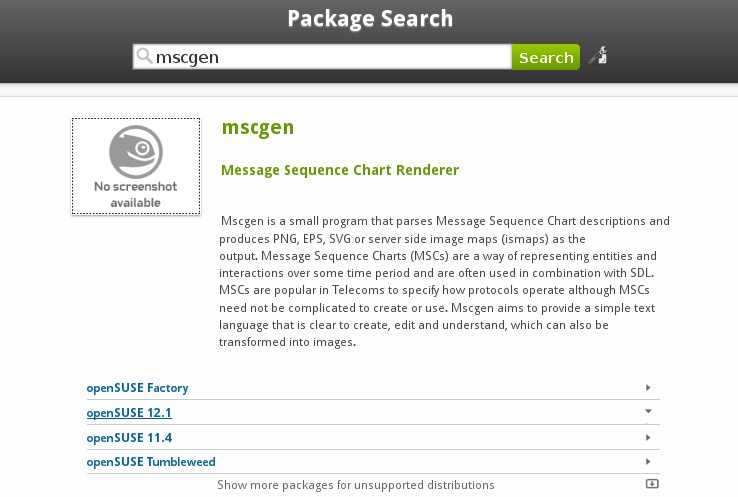
\includegraphics[width=0.5\textwidth]{images/write/graph/mscgen/install-OpenSuse-1}
	\caption[جستجوی نرم‌افزار \lr{mscgen} در موتور جستجوی \lr{OpenSuse}]{
		پس از جستجوی نرم‌افزار \lr{mscgen} و با استفاده از امکان‌های فراهم شده می‌توان
		به سادگی نرم‌افزاری مورد نظر را نصب و راه اندازی کنید.
	}
	\label{images/write/graph/mscgen/install-OpenSuse-1}
\end{figure}

همانگونه که در شکل \ref{images/write/graph/mscgen/install-OpenSuse-1} نمایش داده
شده است امکان نصب نرم‌افزار با تنها یک کلیک فراهم شده است. با انتخاب نرم‌افزار
برای نصب یک دریچه محاوره‌ای (که در شکل
\ref{images/write/graph/mscgen/install-OpenSuse-2} نمایش داده شده است) باز
می‌شود که اطلاعات ابتدایی مخزن نرم افزار را نمایش می دهد. پس از اطمینان یافتن از
مسیر و نوع مخزن دکمه \lr{Next} را کلیک کنید.

\begin{figure}
	\centering
	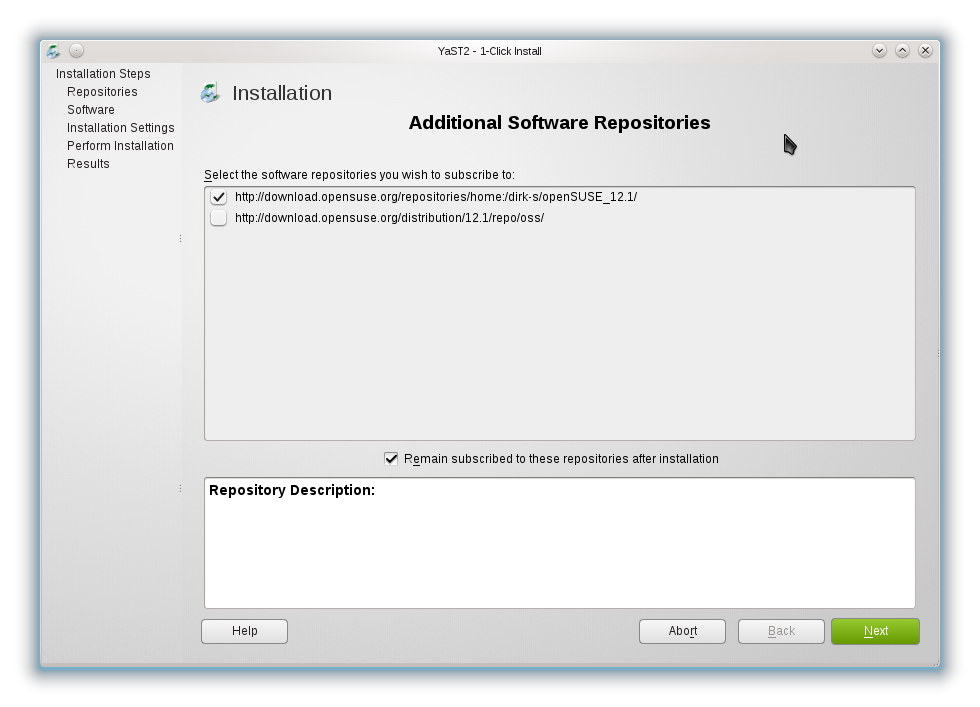
\includegraphics[width=0.5\textwidth]{images/write/graph/mscgen/install-OpenSuse-2}
	\caption[اطلاعات مخزن نرم‌افزاری برای نصب \lr{mscgen}]{
		در این دریچه محاوره‌ای علاوه بر نمایش آدرس، نوع مخزن نرم‌افزاری نیز نمایش داده
		می‌شود. پیش از نصب نرم‌افزار به آدرس و نوع آن توجه کنید.
	}
	\label{images/write/graph/mscgen/install-OpenSuse-2}
\end{figure}

در دریچه محاوره‌ای بعد اطلاعات بسته‌ نرم‌افزاری انتخاب شده برای نصب نمایش داده
می‌شود. این اطلاعات شامل نام و یک توصیف مختصر در مورد نرم افزار است. در شکل
\ref{images/write/graph/mscgen/install-OpenSuse-3} نیز اطلاعات و نام نرم‌افزار
\lr{mscgen} قابل مشاهده است. توجه داشته باشید که در این فهرست تنها همین
نرم‌افزار موجود بوده و برای نصب انتخاب شده باشد. پس از اطمینان حاصل کردن از
اطلاعات نرم‌افزار دکمه \lr{Next} را کلیک کنید.

\begin{figure}
	\centering
	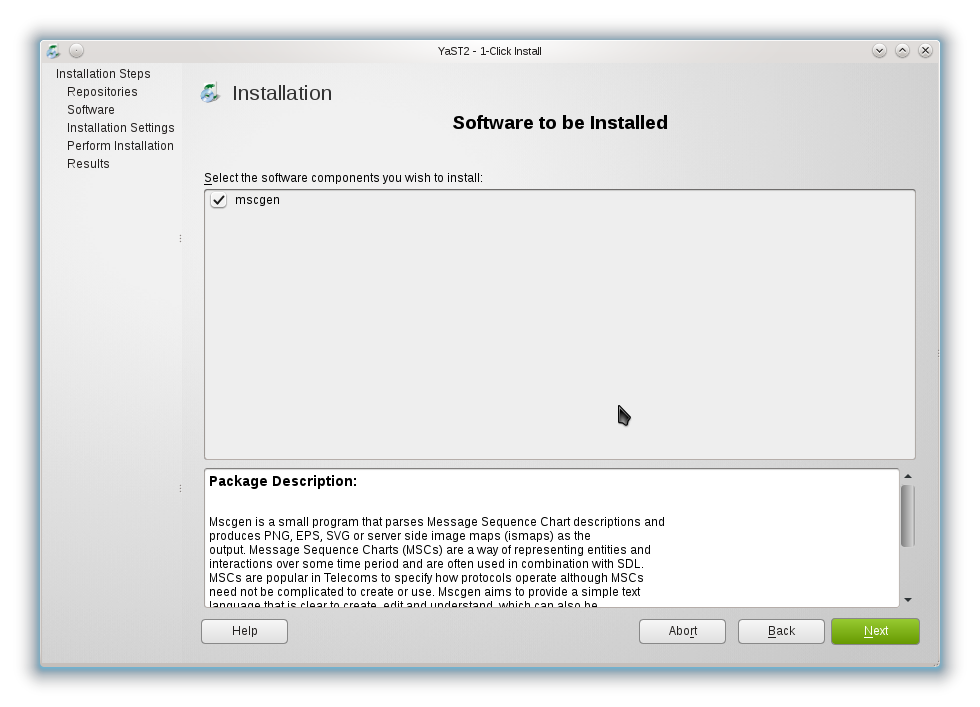
\includegraphics[width=0.5\textwidth]{images/write/graph/mscgen/install-OpenSuse-3}
	\caption[اطلاعات نرم‌افزار \lr{mscgen}]{
		در این دریچه محاوره‌ای اطلاعات کلی بسته \lr{mscgen} نمایش داده شده است. در بخش
		اول این دریچه محاوره‌ای فهرست نرم‌افزارها و در بخش انتهایی توضیحات نرم‌افزار
		انتخاب شده نمایش داده شده است.
	}
	\label{images/write/graph/mscgen/install-OpenSuse-3}
\end{figure}

پس از تایید مخزن‌های نرم‌افزاری و نرم افزارهای مورد نظر فرآیند نصب قابل اجرا
خواهد بود اما پیش از آن در یک دریچه محاوره‌ای خلاصه تمام اطلاعات برای تایید
نهایی نمایش داده می‌شود. همانگونه که در شکل \ref{images/write/graph/mscgen/install-OpenSuse-4}
نمایش داده شده است در این دریچه پایانی فهرستی از تمام داده‌های مورد استفاده در
فرآیند نصب نمایش داده می‌شود. در صورتی که این اطلاعات با اطلاعات مورد نظر شما
تطابق داشت دکمه \lr{Next} را برای ادامه فرآیند کلیک کنید.

\begin{figure}
	\centering
	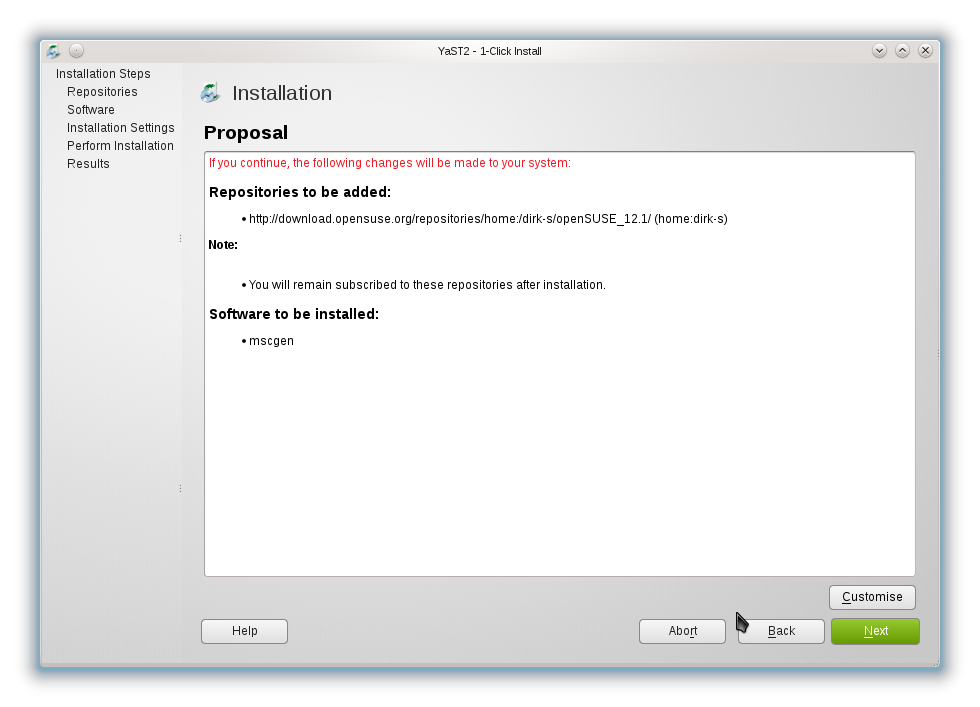
\includegraphics[width=0.5\textwidth]{images/write/graph/mscgen/install-OpenSuse-4}
	\caption[اطلاعات کلی فرآیند نصب نرم‌افزار \lr{mscgen}]{
		دریچه محاوره‌ای شامل تمام اطلاعات نرم افزارها و مخزن‌های مورد استفاده بوده و
		اخرین دریچه محاوره‌ای است که پیش از فرایند نصب نمایش داده می شود.
	}
	\label{images/write/graph/mscgen/install-OpenSuse-4}
\end{figure}

در سیستم‌های لینوکس کاربران سیستم اجازه نصب نرم‌افزار جدید را نداشته و تنها
کاربر اصلی سیستم می‌تواند یک نرم‌افزار جدید را در سیستم نصب کند. از این رو
اگر فرآیند نصب توسط یک کاربر عادی فراخوان شده باشد یک دریچه محاوره‌ای دیگر برای
دریافت گذرواژه نمایش داده می‌شود. در شکل
\ref{images/write/graph/mscgen/install-OpenSuse-5} این دریچه نمایش داده شده
است. گذرواژه کاربر ریشه را وارد و دکمه \lr{Ok} را کلیک کنید.

\begin{figure}
	\centering
	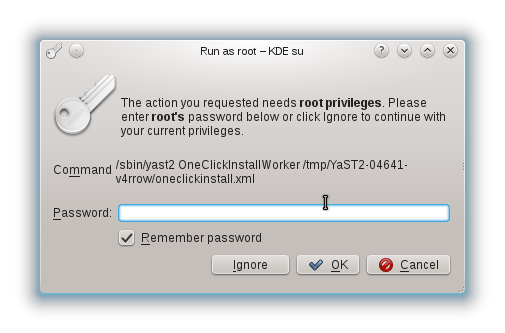
\includegraphics[width=0.5\textwidth]{images/write/graph/mscgen/install-OpenSuse-5}
	\caption[احراز اصالت برای نصب نرم‌افزار \lr{mscgen}]{
		در این دریچه محاوره‌ای علاوه بر بیان درخواست اصلی کاربر، از او خواسته می‌شود
		که گذرواژه کاربر اصلی را وارد کند. تنها کاربر اصلی سیستم می‌تواند نرم‌افزار
		جدید را در سیستم نصب کند.
	}
	\label{images/write/graph/mscgen/install-OpenSuse-5}
\end{figure}

در نهایت فرآیند نصب نرم‌افزار شروع خواهد شد. در این فرآیند نه تنها خود نرم‌افزار
بلکه بسته‌های مورد نیاز در آن \glspl{download} شده و نصب می‌شود. فرآیند و پیشرفت
نصب در یک دریچه محاوره‌ای نمایش داده می‌شود که در شکل
\ref{images/write/graph/mscgen/install-OpenSuse-6} نمایش داده شده است. با
استفاده از این دریچه محاوره‌ای نه تنها پیشرفت کار مشخص است بلکه امکان لغو آن نیز وجود دارد.

\begin{figure}
	\centering
	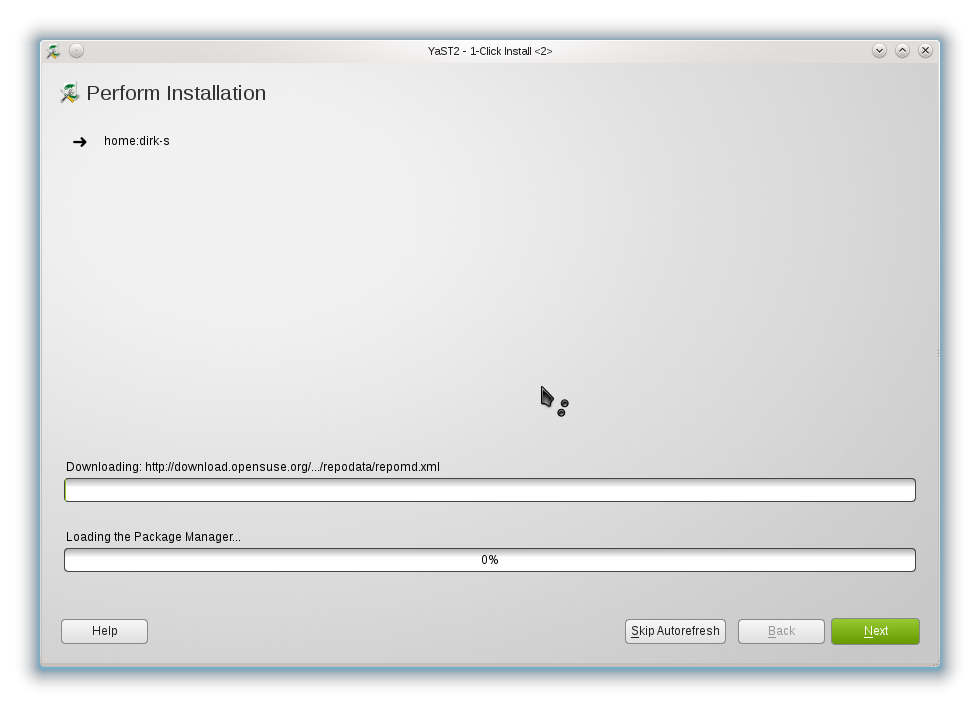
\includegraphics[width=0.5\textwidth]{images/write/graph/mscgen/install-OpenSuse-6}
	\caption[فرآیند نصب نرم‌افزار \lr{mscgen}]{
		در این دریچه محاوره‌ای نه تنها میزان پیشرفت کار نمایش داده شده بلکه امکان‌های
		جنبی مانند راهنما و لغو نصب نیز وجود دارد.
	}
	\label{images/write/graph/mscgen/install-OpenSuse-6}
\end{figure}

در پایان بسته‌های مورد نیاز و برنامه‌های احرایی نصب شده و دستورهای مناسب به
سیستم اضافه خواهد شد. برای بررسی نصب کامل این ابزار در \glspl{terminal program} دستور
\lr{mscgen} را وارد کنید. با صادر کردن این دستور در صورتی که نرم‌افزار به صورت
کامل نصب شده باشد خروجی زیر در \lr{terminal} نمایش داده می‌شود.

\begin{Shell}
> mscgen
-T <type> must be specified on the command line                                                         
Usage: mscgen -T <type> [-o <file>] [-i] <infile>                                                       
       mscgen -l                                                                                        

Where:                                                                                                  
 -T <type>   Specifies the output file type, which maybe one of 'png', 'eps',
             'svg' or 'ismap'
 -i <infile> The file from which to read input.  If omitted or specified as
              '-', input will be read from stdin.  The '-i' flag maybe
              omitted if <infile> is specified as the last option on the
              command line.
 -o <file>   Write output to the named file.  This option must be specified if 
              input is taken from stdin, otherwise the output filename
              defaults to <infile>.<type>.  This may also be specified as '-'
              to write output directly to stdout.
 -p          Print parsed msc output (for parser debug).
 -l          Display program licence and exit.

Mscgen version 0.20, Copyright (C) 2010 Michael C McTernan,
                                        Michael.McTernan.2001@cs.bris.ac.uk
Mscgen comes with ABSOLUTELY NO WARRANTY.  This is free software, and you are
welcome to redistribute it under certain conditions; type `mscgen -l' for
details.

PNG rendering by libgd, www.libgd.org
\end{Shell}

\subsubsection{ویندوز}

با توجه به محدودیت‌های موجود در سیستم‌های عمال ویندوز امکان نصب خودکار و به روز
رسانی وحود ندارد. از این رو ابتدا باید نرم‌افزار را \glspl{download} و سپس اقدام
به نصب آن کنید. در ادامه فرض شده است که برنامه نصب این ابزار در دست رس باشد.
برنامه نصب را به روی سیستم خود \glspl{copy} کرده و آن را احرا کنید. با اچرا شدن
برنامه یک دریچه محاوره‌ای همانند شکل \ref{images/write/graph/mscgen/install-win-1}
نمایش داده خواهد شد.
در این دریچه محاوره‌ای اطلاعات کلی نرم‌افزار نمایش داده شده است. دکمه \lr{Next}
را برای ادامه کار کلیک کنید.

\begin{figure}
	\centering
	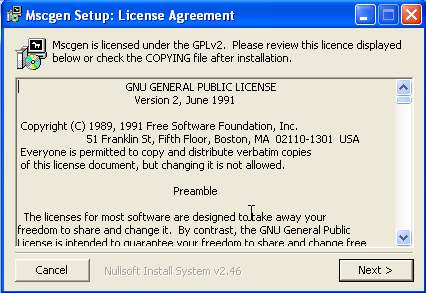
\includegraphics[width=0.5\textwidth]{images/write/graph/mscgen/install-win-1}
	\caption[اطلاعات کلی نرم‌افزار برای نصب در سیستم‌عامل ویندوز]{
		در این دریچه اطلاعاتی ابتدایی نمایش داده شده است. برای نمونه می‌توان به گواهی
		نامه آن اشاره کرد.
	}
	\label{images/write/graph/mscgen/install-win-1}
\end{figure}

در گام بعد دریچه محاوره‌ای برای تعیین پارامترهای مورد نیاز در فرآیند نصب نمایش
داده می‌شود. مهم‌ترین و تنها اطلاعاتی که در این گام باید تعیین شود مسیری است که
\glspl{installer program} داده‌ها را در آن ایجاد خواهد کرد. نمای کلی این دریچه
محاوره‌ای در شکل \ref{images/write/graph/mscgen/install-win-2}
نمایش داده شده است. دکمه \lr{Install} را کلیک کنید.

\begin{figure}
	\centering
	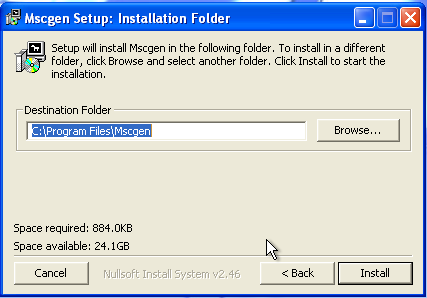
\includegraphics[width=0.5\textwidth]{images/write/graph/mscgen/install-win-2}
	\caption[تنظیم مورد نیاز برای نصب \lr{mscgen} در ویندوز]{
		تنها اطلاعات مورد نیاز برای نصب این نرم‌افزار تعیین مسبی نصب است. با استفاده
		از دکمه \lr{Brows} می‌توانید مسیر مورد نظر خود را تعیین کنید.
	}
	\label{images/write/graph/mscgen/install-win-2}
\end{figure}

در آخرین گام فرآیند نصب، فرآیند نصب آغاز شده و یک دریچه محاوره‌ای نمایش داده
می‌شود. همانگونه که در شکل \ref{images/write/graph/mscgen/install-win-3}
قابل مشاهده است در این دریچه پیشرفت فرایند نصب نمایش داده می‌شود.

\begin{figure}
	\centering
	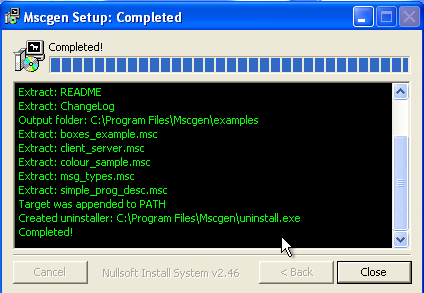
\includegraphics[width=0.5\textwidth]{images/write/graph/mscgen/install-win-3}
	\caption[پیشرفت فرآیند نصب \lr{mscgen} در ویندوز]{
		در این دریچه محاوره‌ای میزان پیشرفت فرآیند نصب نمایش داده می‌شود. پس از پایان
		فرایند نصب دکمه \lr{Close} فعال می‌شود تا با استفاده از آن به فرآیند نصب خاتمه
		داده شود.
		}
	\label{images/write/graph/mscgen/install-win-3}
\end{figure}

در نهایت پس از پایان یافتن این مراحل این ابزار در سیستم نصب شده و قابل استفاده
می‌باشد در اینجا نیز باید دستور \lr{mscgen} به سیستم اضافه شده باشد. برای
اطمینان از این موضوع یک \lr{CMD} باز کرده و در آن این دستور را فراخوانی کنید. با
فراخوانی کردن این دستور باید داده‌های زیر در خروچی نمایش داده شود.

\begin{Shell}
C:\Documents and Settings\malek>mscgen
-T <type> must be specified on the command line
Usage: mscgen -T <type> [-o <file>] [-i] <infile>
       mscgen -l

Where:
 -T <type>   Specifies the output file type, which maybe one of 'png', 'eps',
             'svg' or 'ismap'
 -i <infile> The file from which to read input.  If omitted or specified as
              '-', input will be read from stdin.  The '-i' flag maybe
              omitted if <infile> is specified as the last option on the
              command line.
 -o <file>   Write output to the named file.  This option must be specified if
              input is taken from stdin, otherwise the output filename
              defaults to <infile>.<type>.  This may also be specified as '-'
              to write output directly to stdout.
 -p          Print parsed msc output (for parser debug).
 -l          Display program licence and exit.

Mscgen version 0.20, Copyright (C) 2010 Michael C McTernan,
                                        Michael.McTernan.2001@cs.bris.ac.uk
Mscgen comes with ABSOLUTELY NO WARRANTY.  This is free software, and you are
welcome to redistribute it under certain conditions; type `mscgen -l' for
details.

PNG rendering by libgd, www.libgd.org
\end{Shell}

در این حالت این ابزار در سیستم نصب شده و در درسترس دیگر ابزارها برای تولید مستند
قرار دارد.

\subsection{\lr{Graphviz}}

\lr{Graphviz} روشی برای نمایش داده‌های ساختار یافته به صورت نمودار و گراف است.
از آنجا که بسیاری از شاخه‌های علوم همواره با داده‌های ساختار یافته در ارتباط
بوده و نمایش داده‌ها از اهمیت خاصی برخوردار است، \lr{Graphviz} به عنوان یک ابزار
بسیار کاربردی در انها مطرح است. از این میان می‌توان با شبکه،
\glspl{bioinformatics}، مهندسی رایانه، ساختمان داده، طراحی \glspl{web}،
\glspl{machine learning} و بسیاری دیگر اشاره کرد.

این نرم‌افزار یک نرم‌افزار \glspl{open source} بوده و به روی سکوهای متفاوتی
مانند لینوکس و ویندوز قابل استفاده است. این نرم‌افزار از لایه بندی‌های متفاوتی
برای ترسیم گراف‌ها، به صورت پیش فرض استفاده می‌کند. از طرفی ابزارهای مناسبی برای
کار به روی \glspl{web}، کتابخانه‌ها، زبان‌های برنامه سازی فراهم شده است.

روال کلی این نرم‌افزار به این صورت است که در ابتدا کاربر با استفاده از زبان‌های
ساده و متنی گراف و نمودار خود را توصیف می‌کند، پس از آن این توصیف با استفاده از
این ابزار به صورت یک نمایش و نمودار تبدیل شده و در قالب‌های متفاوتی مانند
\gls{SVG}، \gls{PDF} و یا قالب‌های دیگر ذخیره می‌شود.

توانایی به کارگیر تنظیم‌های متفاوت مانند رنگ، قلم، لایه بندی، طرح خط‌ها،
نمایش‌ها و دیگر موارد این ابزار را به یک ابزار بسیار کاربردی در طراحی و ایجاد
نمودارها مبدل ساخته است.

در عمل این ابزار به گونه‌ای طراحی شده است که داده‌های ساختار یافته را به عنوان
داده ورودی دریافت کرده و بر اساس دستورهای خاص آنها را ترسیم کند اما این به آن
معنی نیست که قادر به ترسیم نمودارهای دیگر نباشد. به بیان دیگر این امکان نیز
فراهم شده است که کاربر تنها نمایش و ترسیم را تعیین کرده و داده‌های ورودی مورد
نظر خود را به عنوان پارامتر در آن وارد کند.

در این بخش روش نصب و به کار گیری ابن نرم‌افزار به روی سکوهای متفاوتی مانند
لینوکس و ویندوز تشریح خواهد شد و در ادامه روش به کارگیر این نرم‌افزار در مستند
سازی تکنیکی مورد بررسی قرار خواهد گرفت.

\subsubsection{لینوکس}
در این قسمت به نحوه نصب \lr{Graphviz} بر روی سیستم عامل لینوکس با توزع \lr{SUSE} اشاره خواهد شد.
مانند روش نصب همه نرم افزارها و بسته‌های مورد استفاده در لینوکس، جهت نصب \lr{Graphviz} نیز ابتدا مانند شکل زیر باید به بخش مدیریت نرم افزارها در لینوکس رفت.

\begin{figure}
	\centering
	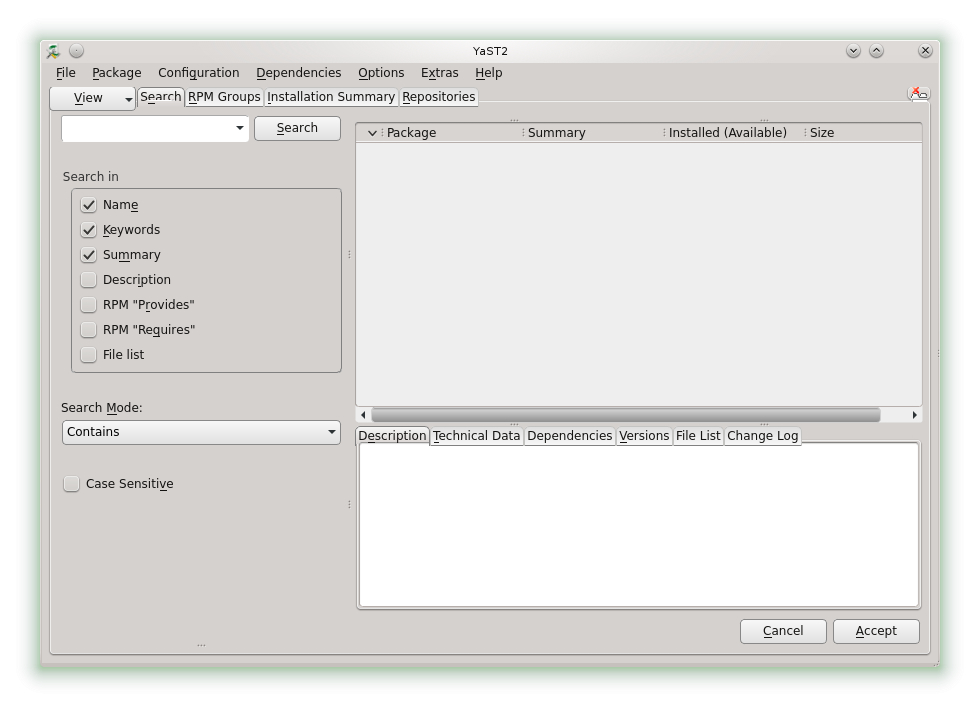
\includegraphics[width=0.5\textwidth]{images/write/graph/graphviz/install-OpenSUSE-0}
	\caption[]{بخش مدیریت نرم افزارها در لینوکس}
	\label{images/write/graph/graphviz/install-OpenSUSE-0}
\end{figure}

در قسمت جستجوی نرم افزار مورد نظر نام \lr{Graphviz} را وارد کنید. همانطورد که در پنجره سمت راست حاصل از نتایج جستجو دیده می‌شود تمام نرم افزارها و بسته‌های مختلف حاصل مربوط به کلمه فوق دیده می‌شود. با انتخاب \lr{Graphviz} و علامت زدن آن، نرم افزار مورد نظر و تمام بسته‌های مورد نیاز در سیستم نصب می‌شوند.
\begin{figure}
	\centering
	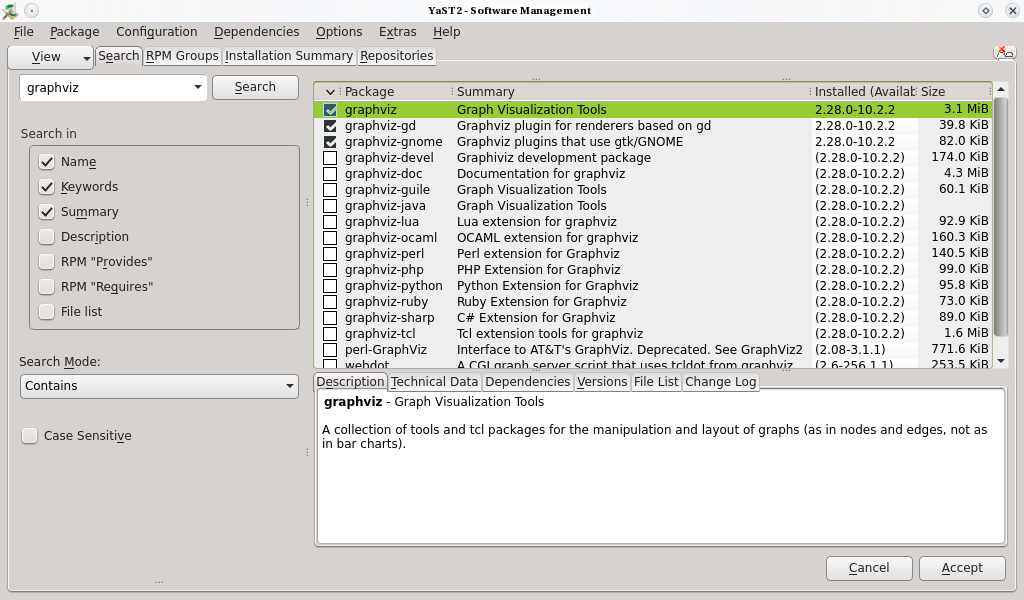
\includegraphics[width=0.5\textwidth]{images/write/graph/graphviz/install-OpenSUSE-1}
	\caption[]{بخش جستجو و نصب نرم افزار مورد نظر
	
	}
	\label{images/write/graph/graphviz/install-OpenSUSE-1}
\end{figure}
در انتها فرایند نصب نرم افزار و تمام بسته‌های مورد نیاز نرم افزار تا پایان نصب انجام می‌شود.
\begin{figure}
	\centering
	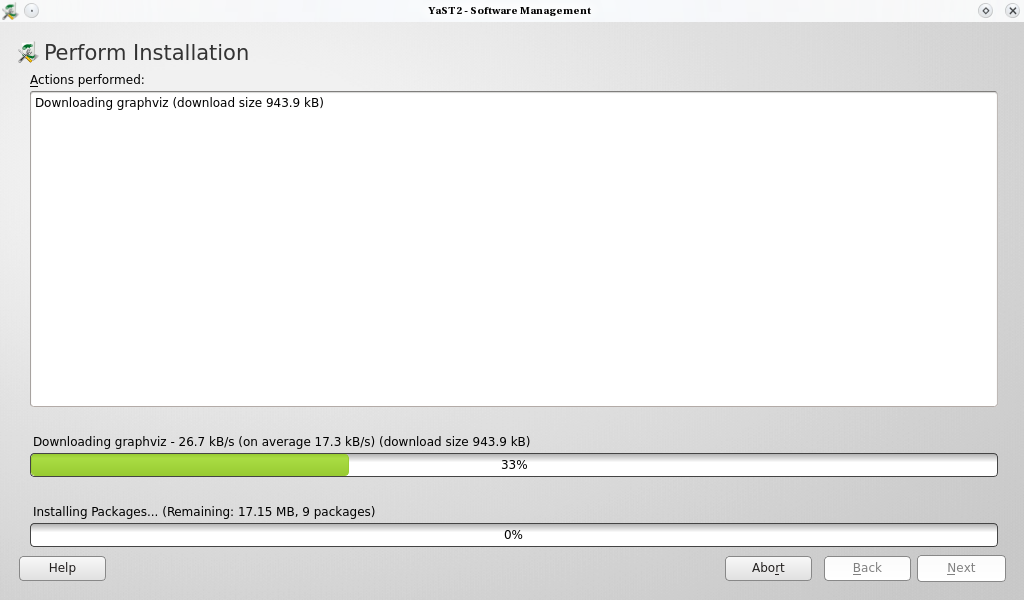
\includegraphics[width=0.5\textwidth]{images/write/graph/graphviz/install-OpenSUSE-2}
	\caption[]{فرآیند نصب نرم افزار
	
	}
	\label{images/write/graph/graphviz/install-OpenSUSE-2}
\end{figure}

\subsubsection{ویندوز}

\begin{webreference}
جهت نصب \lr{Graphviz} بر روی سیتم عامل ویندوز ابتدا باید نرم افزار را دانلود کرد
و سپس آن را نصب کرد. می‌توانید نرم افزار را از سایت زیر دانلود کنید:
\begin{latin}
http://www.graphviz.org/Download\_windows.php
\end{latin}
\end{webreference}

پس از دانلود نرم افزار فوق بر روی آن دوبار کلیک کنید تا فرآیند نصب نرم افزار
شروع شود. در پنجره ظاهر شده اطلاعات کلی از نرم افزار آمده است. برای ادامه روند
نصب بر روی کلید \lr{next} کلیک کنید.

\begin{figure}
	\centering
	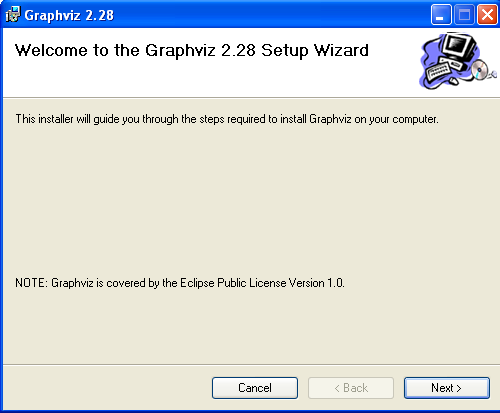
\includegraphics[width=0.5\textwidth]{images/write/graph/graphviz/install-1}
	\caption[]{صفحه اولیه نصب نرم افزار در ویندوز
	
	}
	\label{images/write/graph/graphviz/install-1}
\end{figure}

در پنجره بعد باید مسیری برای نصب نرم افزار انتخاب کرد. همچنین سطح دسترسی برای
استفاده از نرم افزار را مشخص کرده و روند نصب را ادامه داد.

\begin{figure}
	\centering
	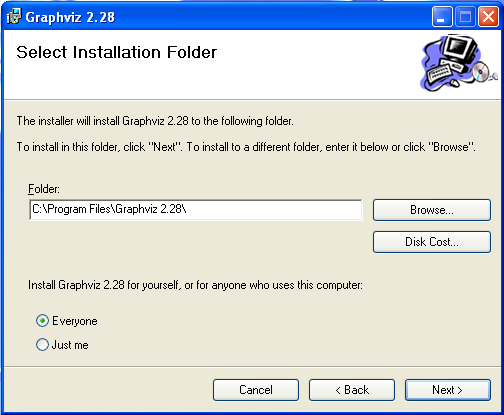
\includegraphics[width=0.5\textwidth]{images/write/graph/graphviz/install-2}
	\caption[]{انتخاب مسیر جهت نصب نرم افزار
	
	}
	\label{images/write/graph/graphviz/install-2}
\end{figure}

در ادامه نصب باید مرحله نصب نهایی نرم افزار را تصدیق کرد تا نرم افزار شروع به
نصب شود. در آخر کلید \lr{close} را جهت اتمام نصب نرم افزار کلیک کنید.
\begin{figure}
	\centering
	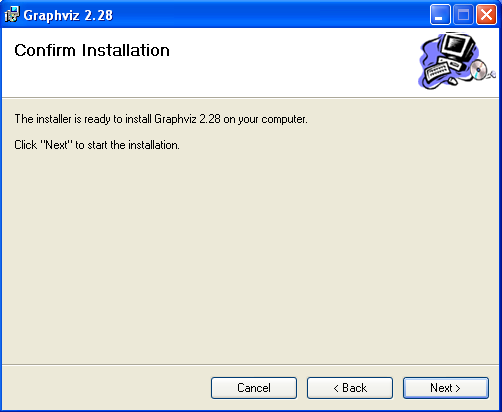
\includegraphics[width=0.5\textwidth]{images/write/graph/graphviz/install-3}
	\caption[]{تایید نهایی نصب نرم افزار
	
}
	\label{images/write/graph/graphviz/install-3}
\end{figure}

پس از نصب کامل برنامه از منوی \lr{start} برنامه نصب شده \lr{GVEdit.exe} را اجرا
کرده تا ویزارد مربوط به \lr{Graphviz} ظاهر شود. در این ویزارد با ایجاد یک پروژه
جدید و در پنجره‌ای که با نام پروژه ظاهر شده است می‌توان کدهای گراف مورد نظر را
اجرا کرد. پس از تکمیل کد نهایی با زدن کلید \lr{F5} صفحه کلید نتیجه کد نوشته شده
در پنجره جداگانه نمایش داده می‌شود که می‌توان آن را در قالب‌های مختلف ذخیره کرد.




%%
% حق نشر 1390-1402 دانش پژوهان ققنوس
% حقوق این اثر محفوظ است.
% 
% استفاده مجدد از متن و یا نتایج این اثر در هر شکل غیر قانونی است مگر اینکه متن حق
% نشر بالا در ابتدای تمامی مستندهای و یا برنامه‌های به دست آمده از این اثر
% بازنویسی شود. این کار باید برای تمامی مستندها، متنهای تبلیغاتی برنامه‌های
% کاربردی و سایر مواردی که از این اثر به دست می‌آید مندرج شده و در قسمت تقدیر از
% صاحب این اثر نام برده شود.
% 
% نام گروه دانش پژوهان ققنوس ممکن است در محصولات دست آمده شده از این اثر درج
% نشود که در این حالت با مطالبی که در بالا اورده شده در تضاد نیست. برای اطلاع
% بیشتر در مورد حق نشر آدرس زیر مراجعه کنید:
% 
% http://dpq.co.ir/licence
%
\section{\lr{Mscgen}}

همانگونه که پیش از این اشاره شده با استفاده از این ابزار می‌توان \glspl{message
sequence chart} را در مستند‌ها ایجاد کرد و به خوانایی مستند‌های ایجاد شده افزود.
یک \glspl{message sequence chart} را در مستند می‌توان به دو روش متفاوت ایجاد
کرد. در روش اول با استفاده از برچسب \lr{msc} می‌توان در لابه‌لای مستندهای تکنیکی
نوشته شده نمودارها مورد نیاز ایجاد کرد. استفاده از این دستور امکان بیان جزئیات
کامل \glspl{message sequence chart} را در خود مستند فراهم می‌کند. ساختار کلی این
دستور به صورت زیر است.
 
\begin{C++}
/**
 * \msc
 * [Diagram detail]
 * \endmsc
 */
\end{C++}

با استفاده از این قالب، قمست مستند ایجاد شده به عنوان یک توصیف صحیح از یک
\glspl{message sequence chart} در نظر گرفته می‌شود. همانگونه که این قالب کلی
قابل مشاهده است توصیف نمودار می‌بایست در محدوده ایجاد شده دو دستور \lr{msc} و
\lr{endmsc} قرار گیرد. قراردادهای توصیف نمودار در انتهای این بخش مورد بررسی قرار
گرفته شده است.

\begin{note}
برای استفاده از این دستورها باید بر اساس قراردادها و زبان توصیف نمودار، \glspl{}
را به صورت کامل و بدون اشتباه در میان این دو دستور نوشته شود. در صورتی که
اشتباهی در این توصیف وجود داشده باشد \glspl{documenter} از آن صرف نظر خواهد کرد.
\end{note}

برای نمونه فرض کنید که قراردادی وجود دارد که در آن یک طرف دستوری را ارسال کرده و
دیگری نتیجه اجرای دستور را گزارش می‌دهد. نمودار این قرارداد در نمونه زیر ایجاد
شده است.

\begin{C++}
/**
 * \msc
 * Sender,Receiver;
 * Sender->Receiver [label="Command()"];
 * Sender<-Receiver [label="Ack()"];
 * \endmsc
 */
\end{C++}

با یک دید نه تنها می‌توان مفاهیم به کار رفته در این توصیف را درک کرد بلکه به این
نکته اذعان کرد که توصیف نمودار بسیار شبه به همان توصیف قرارداد خواهد بود. این
شباهت در توصیف یک قرارداد و توصیف نمودار آن یکی از مهم‌ترین خصوصیت‌های این دستور
است.

% maso 1391: تنظیم‌های کلی برای استفاده از دستور

فرآیند کلی تولید یک \glspl{message sequence chart} با استفاده از این دستور به
این قرار است: در گام نخست کاربر توصیف کامل نمودار را در مستند ایجاد کرده و
\lr{Doxygen} را برای تولید مستند نهایی فراخوانی می‌کند، \glspl{documenter} با
مشاهده این دستور توصیف نمودار را استخراج کرده و با استفاده از ابزار \lr{mscgen}
آن را به \glspl{message sequence chart} معادل ترجمه می‌کند و در نهایت نمودار
ایجاد شده را در مستند نهایی ایجاد شده قرار می‌گیرد. در این فرآیند
\glspl{documenter} با استفاده از ابزار جانبی \lr{mscgen} نمودارهای مورد نیاز
کاربر را ایجاد کرده و در در فرآیند تولید مستند نهایی استفاده می‌کند از این رو
باید روشی برای فراخوانی و استفاده از این ابزار برای \glspl{documenter} فراهم
شود. زمانی که ابزار \lr{mscgen} به صورت سیستمی نصب شده باشد و دستور آن به عنوان
یک دستور جدید در کل سیستم قابل دسترسی باشد \lr{Doxygen} به صورت خودکار آن را
تشخیص داده و از آن استفاده می‌کند، اما مشکل اساسی زمانی رخ می‌دهد که این ابزار
به صورت محلی نصب شده و به عنوان یک دستور معرفی نشده باشد. در این حالت با استفاده
از گزینه \lr{MSCGEN\_PATH} می‌توان مسیر این ابزار را برای \glspl{documenter}
تعیین کرد. حالت کلی استفاده از این گزینه در تنظیم‌های مستند به صورت زیر است:

\begin{Shell}
MSCGEN_PATH = <path to mscgen>
\end{Shell}

زمانی که این خصوصیت در پیکره بندی مستند تعریف نشده باشه \glspl{documenter} به
صورت خودکار در مسیرهای استاندارد به دنبال این ابزار جستجو خواهد کرد.

%maso 1391: استفاده از پرونده به عنوان نمودار
اما استفاده از دستور \lr{msc} و توصیف نمودار در خود مستند تنها روش ایجاد
\glspl{message sequence chart} نیست. یک روش بسیار مناسب و پرکاربرد توصیف نمودار
در پرونده‌های جداگانه و استفاده از دستور \lr{mscfile} است. با استفاده از این
دستور می‌توان یک پرونده شامل توصیف یک نمودار را به مستند اضافه کرد. ساختار کلی
این دستور به صورت زیر است:

\begin{C++}
 /**
  * \mscfile <file> ["caption"]
  */
\end{C++}

نخستن پارامتر ورودی این برچسب مسیر پرونده‌ای را که توصیف نمودار در
آن ایجاد شده است و پارامتر دوم زیر نویس نمودار ایجاد شده را تعیین
می‌کنند. پرونده تعیین شده به عنوان نمودار باید در مسیرهایی ایجاد شده باشد که در
پرونده پیکره بندی مشخص شده است. تعیین مسیر پرونده‌های مورد استفاده در این دستور
با استفاده از برچسب \lr{MSCFILE\_DIRS} در پرونده پیکره بندی تعیین می‌شود.

\begin{note}
مسیر پرونده در این دستور نمی‌تواند شامل \glspl{space} باشد، در این حالت مسیر را
باید در میان کوتیشن نوشت. این روش در حالت کلی به صورت زیر است:
\begin{C++}
 /**
  * \mscfile "<file path>" ["caption"]
  */
\end{C++}
\end{note}

%TODO: maso 1391: تنظیم‌های پرونده‌ها

% TOTO: hadi 1391: در مورد ساختار کلی توصیف نمودار
% TOTO: hadi 1391: در مورد نوشتن توضیحات در متن کدهای mscgen

\subsection{موجودیت‌ها}

% arcskip
% IDURL
% ID
% URL
% label

% Lists the entities that will be used in the message sequence chart, in the order
% in which they should appear left to right and horizontally across the page. Note
% that each entity name can or may not be quoted, unless the name is to include a
% space, in which case double quotes are required.
% 
% 
% arctextbgcolour, arctextbgcolor
% arctextcolour, arctextcolor
% arclinecolour, arclinecolor

هر موجودیت در سیستم می‌تواند به موجودیت‌های دیگر سیستم پیام بدهد یا پیامی از
آن‌ها دریافت کند. در واقع موجودیت‌ها نقش اصلی را در \glspl{message sequence
chart} دارند. بنابراین قبل از هر کاری باید موجودیت‌های نمودار را تعیین کرد. برای
تعریف یک موجودیت در نمودار کافی است نام مورد نظر برای موجودیت را بنویسید و پس از
آن یک علامت نقطه ویرگول ($;$) قرار دهید. برای تعریف چند موجودیت هم باید از کاما
استفاده شود. نکته مهم اینکه تعریف موجودیت‌ها را نباید با نقطه ویرگول از هم جدا
کرد و فقط بعد از آخرین موجودیت علامت نقطه ویرگول گذاشته می‌شود. در نموداری که
توسط ابزار \lr{Mscgen} تولید می‌شود موجودیت‌ها از سمت چپ به راست و به همان
ترتیبی که در هنگام تعریف آورده شده‌اند قرار می‌گیرند. در کد زیر نحوه تعریف
موجودیت‌ها نشان داده شده است:

\begin{MSC}
msc {
	entity1, entity2, ... ,	entityn;
	
	# Definition of message(s)
	
}
\end{MSC}

در این کد به تعداد دلخواه موجودیت تعریف کرده‌ایم. همانطور که به راحتی می‌توان از
کد فهمید برای تعریف هر موجودیت کافی است نامی که می‌خواهیم به موجودیت بدهیم را
بیان کنیم. فرض کنید نموداری را به صورت زیر توصیف کرده باشیم:

\begin{MSC}
msc {
	e1, e2, e3;
	
	e1->e2;	
}
\end{MSC}

در تصویر \ref{images/write/graph/mscgen/entity-example-1} نمایی از آنچه توسط
ابزار \lr{Mscgen} برای کد بالا تولید می‌شود نشان داده شده است. توجه شود که در کد
مربوط به این تصویر تنها سه موجودیت را تعریف کرده‌ایم و در نمودار تولید شده
موجودیت‌ها از چپ به راست با همان ترتیبی که در تعریف آمده‌اند قرار گرفته‌اند.

\begin{note}
دستور $e1->e2$ توصیف یک پیام از موجودیت \lr{e1} به موجودیت \lr{e2} است که در 
تصویر \ref{images/write/graph/mscgen/entity-example-1} نیز یک فلش از موجودیت اول
به موجودیت دوم دیده می‌شود.در قسمت~\ref{sec:message} انواع پیام‌ها و توصیف آن‌ها
به طور کامل شرح داده شده است.
در اینجا فقط برای اینکه بتوانیم نمودار مورد نظر را تولید کنیم یک پیام را تعریف کرده‌ایم
چون همانطور که قبلا گفته شد در توصیف نمودار باید حداقل یک موجودیت و حداقل یک پیام تعریف شده باشد.
در غیر این صورت ابزار \lr{Mscgen} با خطا مواجه شده و نمودار مربوطه را تولید نمی‌کند.
\end{note}

\begin{figure}[h]
	\centering
	\includegraphics[width=0.85\textwidth]{images/write/graph/mscgen/entity-example-1}
	\caption[مثالی از نحوه نمایش موجودیت‌ها توسط ابزار \lr{Mscgen}]
	{در این شکل سه موجودیت تعریف شده است. ابزار \lr{Mscgen} برای کد تعریف کننده این موجودیت‌ها 
	تصویری به این صورت نشان می‌دهد.}
	\label{images/write/graph/mscgen/entity-example-1}
\end{figure}

\begin{note}
موجودیت در \lr{UML} با عنوان \lr{life time} شناخته می‌شود.
\end{note}

اگر در نامی که می‌خواهید برای موجودیت خود بگذارید خط فاصله (فضای خالی) وجود
داشته باشد باید نام مورد نظر را بین دو علامت گیومه (\lr{"}) قرار دهید. مثلا فرض
کنید بخواهیم موجودیت‌هایی با نام‌های \lr{Entity One} و \lr{Entity Two} تعریف
کنیم برای این کار باید کد زیر را بنویسید:

\begin{MSC}
msc {
	"Entity One", "Entity Two";
	
	# Defenition of message(s)
}
\end{MSC}

حال فرض کنید نامی طولانی برای موجودیت خود گذاشته‌اید. در این صورت هر بار بخواهید
به این موجودیت ارجاعی داشته باشید (مثلا رابطه‌ای بین آن و یک موجودیت دیگر برقرار
کنید) مجبورید نام آن موجودیت را به طور کامل بیان کنید. به کد زیر توجه کنید:

\begin{MSC}
msc {
	"Entity Number one", "Entity Number two";
	
	"Entity Number one"->"Entity Number two";
}
\end{MSC}

خروجی ابزار \lr{Mscgen} برای این کد در تصویر
\ref{images/write/graph/mscgen/entity-example-2} نشان داده شده است.

\begin{figure}[h]
	\centering
	\includegraphics[width=0.85\textwidth]{images/write/graph/mscgen/entity-example-2}
	\caption[مثالی از نحوه تعریف موجودیت‌هایی با نام‌های طولانی و حاوی خط فاصله]
	{در این شکل خروجی ابزار \lr{Mscgen} برای کد مربوط به تعریف موجودیت‌هایی با نام طولانی نشان داده شده است.}
	\label{images/write/graph/mscgen/entity-example-2}
\end{figure}

برای پرهیز از این کار روش دیگری برای تعریف موجودیت وجود دارد. در این روش یک
موجودیت به همراه یک برچسب خاص تعریف می‌شود. نمونه‌ای از این روش تعریف موجودیت در
کد زیر آورده شده است:

\begin{MSC}
msc {
	a[label="Entity Number one"], b[label="Entity Number two"];
	
	a->b;
}
\end{MSC}

همانطور که در کد بالا دیده می‌شود دستور تعریف موجودیت به این صورت است: ابتدا
نامی که می‌خواهید qبرای ارجاعات بعدی در کد از آن استفاده کنید، سپس بین دو کروشه
ابتدا کلمه \lr{label}، سپس علامت مساوی (=) و در مقابل آن نامی که می‌خواهید در
دیاگرام تولیدی توسط ابزار \lr{Mscgen} برای موجودیت مورد نظر ظاهر شود. در واقع با
این کار برای موجودیت‌ها خصوصیت \lr{label} را تعریف کرده و مقداردهی می‌کنید. در این
روش هم برای تعریف چند موجودیت باید از کاما استفاده کرد و در انتهای تعریف
موجودیت‌ها نقطه‌ویرگول قرار داده شود.

نمودار مربوط به کد اخیر دقیقا مثل نمودار کد قبلی (تصویر
\ref{images/write/graph/mscgen/entity-example-2}) است. اما مشاهده می‌شود که
تعریف پیام‌ها در کد دوم چقدر ساده‌تر و سریع‌تر از کد قبل است.

% TODO: hadi 1391: تعریف خصوصیات مربوط به یک موجودیت
یک موجودیت علاوه بر خصوصیت \lr{label} خصوصیات دیگری نیز دارد که می‌توان آن‌ها را با
مقادیر دلخواه مقداردهی کرد. با خصوصیات مختلف یک موجودیت می‌توان موادی چون رنگ متن
مربوط به نام موجودیت، رنگ پس‌زمینه نام موجودیت، رنگ خط زمانی یا همان
\lr{time-line} موجودیت و \lr{\ldots} را تعیین کرد. به طور کلی برای مقداردهی
خصوصیات مختلف یک موجودیت باید هنگام تعریف موجودیت در مقابل نام آن و بین دو علامت کروشه
([]) خصوصیت مورد نظر را ذکر کرده و مقداری دلخواه خود را به آن خصوصیت بدهید. خصوصیات مختلف
باید با کاما از یکدیگر جدا شوند. شکل کلی مقداردهی به خصوصیات یک موجودیت به این صورت
است:

\begin{MSC}
msc {
	entity1[attribute1="value1" , attribute2="value2" , ... ,
	attribute="value"],
	entity2[attribute1="value1", attribute2="value2", ... ,
	attribute="value"];
	.
	.
	# Definition of messages
	.
	.
}
\end{MSC}

با استفاده از خصوصیت \lr{linecolor} یا \lr{linecolour} می‌توان رنگ خط زمانی
موجودیت را به رنگ دلخواه تغییر داد. با استفاده از خصوصیت \lr{textcolor} یا
\lr{textcolour} نیز می‌توان رنگ متن مربوط به نام موجودیت را تغییر داد و
با استفاده از خصوصیت \lr{textbgcolor} یا \lr{textbgcolour} می‌توان رنگ پس‌زمینه
نام موجودیت را تعیین کرد. لازم به ذکر است که این خصوصیات برای پیام‌ها نیز تعریف
تعریف شده که در بخش~\ref{sec:message} شرح داده شده‌اند. به کد زیر و تصویر معادل
تولید شده توسط ابزار \lr{Mscgen} برای این کد (تصویر \ref{images/write/graph/mscgen/entity-example-3}) توجه نمایید.

\begin{MSC}
msc {
	 a[label="Entity A", linecolor="green", textcolor="red", textbgcolor="yellow"],
	 b[label="Entity B", linecolor="blue", textcolor="#800000", textbgcolor="#c0c0c0"],
	 c[label="Entity C"];
	 
	 a->b;
  	 b->c;
  	 c->c;
  	 a<-c;
  	 a<-b;
}
\end{MSC}

\begin{figure}[h]
	\centering
	\includegraphics[width=0.85\textwidth]{images/write/graph/mscgen/entity-example-3}
	\caption[مثالی از نحوه تعریف خصوصیات مختلف موجودیت‌ها]
	{در این شکل خروجی ابزار \lr{Mscgen} برای کد مربوط به تعریف خصوصیات
	مختلف رنگی موجودیت‌ها نشان داده شده است.}
	\label{images/write/graph/mscgen/entity-example-3}
\end{figure}
 
رنگ قسمت‌های مختلف کلیه پیام‌هایی که از یک موجودیت شروع می‌شوند را نیز می‌توان
در خصوصیات مربوط به همان موجودیت کنترل کرد. با استفاده از خصوصیت
\lr{arclinecolor} یا \lr{arclinecolour} یک موجودیت می‌توان رنگ پیکان تمام
پیام‌هایی که از آن موجودیت شروع می‌شوند را تعیین کرد. به عبارتی با تعیین رنگ
برای این خصوصیت از موجودیت، رنگ پیش‌فرض تمام پیکان‌هایی که از آن موجودیت شروع
می‌شوند را تعیین کرده‌اید. البته می‌توان با تعیین خصوصیت \lr{linecolor} از یک
پیام خاص، رنگ آن پیکان آن پیام را تغییر داد تا از این رنگ پیش‌فرض استفاده نکند.
علاوه بر آن با استفاده از خصوصیت \lr{arctextcolor} یا \lr{arctextcolour} نیز
می‌توان رنگ متن پیام‌هایی که از یک موجودیت شروع می‌شوند را تغییر داد (رنگ متنی
که معمولا در بالای پیکان مربوط به یک پیام قرار می‌گیرد). در این مورد هم با تعیین
رنگ برای این خصوصیت از موجودیت، رنگ متن تمام پیام‌هایی که از آن موجودیت ارسال
می‌شوند را به صورت پیش‌فرض تعیین کرده‌اید.در مورد این خصوصیت هم می‌توان با تعیین
خصوصیت \lr{textcolor} از یک پیام خاص، رنگ متن آن پیام را تغییر داد تا از این رنگ
پیش‌فرض استفاده نکند. همچنین با استفاده از خصوصیت \lr{arctextbgcolor} یا \lr{arctextbgcolour} می‌توان رنگ
پس‌زمینه متن پیام‌هایی که از یک موجودیت شروع می‌شوند را مشخص کرد (رنگ پس‌زمینه
متنی که معمولا در بالای پیکان مربوط به یک پیام قرار می‌گیرد). با تعیین
رنگ برای این خصوصیت از موجودیت، رنگ پس‌زمینه متن تمام پیام‌هایی که از آن موجودیت ارسال می‌شوند را به
صورت پیش‌فرض تعیین کرده‌اید. باز هم می‌توان با تعیین خصوصیت \lr{textbgcolor} از
یک پیام خاص، رنگ پس‌زمینه متن آن پیام را تغییر داد تا از این رنگ پیش‌فرض استفاده
نکند. در زیر یک نمونه کد مثال برای دستکاری این خصوصیات آورده شده است. نمودار
متناظر این کد در تصویر \ref{images/write/graph/mscgen/entity-example-4} آورده
شده است.

\begin{MSC}
msc {
	 a[label="Entity A", arclinecolor="green", arctextcolor="#ffffff", arctextbgcolor="black"],
	 b[label="Entity B", arctextbgcolor="yellow", arctextcolor="#800000"],
	 c[label="Entity C", arclinecolor="blue"];
	 
	 a->b [label="A to B"];
	 a->b [label="A to B (again)"];
	 a->c [label="A to C"];
  	 b->c [label="B to C"];
  	 b->a [label="B to A"];
  	 b->b [label="Cycle on B"];
  	 c->c [label="Cycle on C"];
  	 a<-c;
  	 a<-b [label="reverse()"];
}
\end{MSC}

\begin{figure}[h]
	\centering
	\includegraphics[width=0.85\textwidth]{images/write/graph/mscgen/entity-example-4}
	\caption[مثالی از نحوه تعریف خصوصیات مختلف موجودیت‌ها برای کنترل پیام‌های یک
	موجودیت]
	{در این تصویر نمودار متناظر برای کد مربوط به تعریف خصوصیات
	مختلف رنگی پیام‌های ارسالی از موجودیت‌ها نشان داده شده است.}
	\label{images/write/graph/mscgen/entity-example-4}
\end{figure}

علاوه بر این خصوصیات که تعیین کننده رنگ و ظاهر نمودار نهایی هستند خصوصیات دیگری
نیز برای موجودیت‌ها وجود دارد که با استفاده از آن‌ها می‌توان پیوندها و ارجاعات
را در نمودار مدیریت کرد. با استفاده از خصوصیت \lr{URL} می‌توان پیوندی به
قسمت‌های دیگر مستند و یا به یک تارنما خارج از مستند ایجاد کرد (متن پیوند همان
برچسب موجودیت خواهد بود). وقتی خصوصیت \lr{URL} یک موجودیت مقداردهی شود (مثلا
آدرس یک تارنما به عنوان مقدار به آن داده شود) آنگاه نام موجودیت به صورت یک پیوند
به آن آدرس عمل می‌کند که وقتی خواننده مستند نهایی شما روی آن کلیک کند به آدرس
داده شده هدایت خواهد شد. البته زمانی که از توصیفی اینچنین یک عکس (مثلا در قالب
\lr{png}) تولید شود، این پیوند عمل نمی‌کند و تنها نام موجودیت به رنگ آبی نمایش
می‌یابد. اما هنگامی که از این توصیف برای تولید مستندات از طریق \lr{Doxygen}
استفاده شود نمودارها به صورتی تولید می‌شوند که پیوند مربوطه کار می‌کند. نکته مهم
دیگر این است اگر از توصیف نمودار در مستنداتی که قرار است توسط \lr{Doxygen} تولید
شوند استفاده می‌کنید علاوه بر پیوند به تارنماهای خارج از مستند می‌توانید با
تگ‌‌هایی به صورت \lr{\textbackslash ref\{aaa\}} به محلی در همان مستندات پیوند
ایجاد کنید تا خواننده مستندات با کلیک روی نام موجودیت به آن قسمت از مستندات
هدایت شود. در این تگ عبارت \lr{aaa} محلی در مستند است که می‌خواهید پیوند مورد
نظر به آنجا اشاره کند.

خصوصیت دیگری که برای موجودیت‌ها وجود دارد خصوصیت \lr{ID} است. این خصوصیت در واقع
یک شناسه به صورت بالانویس در مقابل نام موجودیت قرار می‌دهد.
این شناسه ممکن است در پاورقی‌ها (مثلا برای نوشتن توضیحاتی در انتهای متن‌ها و
مستندات) مورد استفاده قرار گیرد. خصوصیت دیگر موجودیت‌ها \lr{IDURL} است. این
خصوصیت دقیقا مثل خصوصیت \lr{URL} عمل می‌کند با این تفاوت که پیوند مربوطه روی
شناسه بالانویسی که در مقابل نام موجودیت است قرار داده می‌شود. نکته مهم اینکه در
صورتی که برای موجودیت خصوصیت \lr{ID} تعریف نشده باشد این خصوصیت کاربردی نخواهد
داشت. به عبارتی این خصوصیت وابسته به تعریف خصوصیت \lr{ID} در موجودیت است. کد زیر
و نمودار معادل آن که در تصویر \ref{images/write/graph/mscgen/entity-example-5}
نشان داده شده یک نمونه مثال برای استفاده از خصوصیات \lr{URL}، \lr{ID} و
\lr{IDURL} در موجودیت‌ها است.

\begin{MSC}
msc {
	 a[label="Arsheet", ID="1", URL="www.arsheet.org"],
	 b[label="My System", ID="2"],
	 c[label="Entity C", ID="id 3", IDURL="www.google.com"];
	 
	 a->b [label="A to B"];
	 a->b [label="A to B (again)"];
	 a->c [label="A to C"];
  	 b->c [label="B to C"];
  	 b->b [label="Cycle on B"];
  	 a<-c;
}
\end{MSC}

\begin{figure}[h]
	\centering
	\includegraphics[width=0.85\textwidth]{images/write/graph/mscgen/entity-example-5}
	\caption[مثالی از نحوه تعریف خصوصیات مختلف موجودیت‌ها برای ایجاد شناسه
	بالانویس و پیوند]
	{در این تصویر نمودار متناظر برای کد مربوط به تعریف
	خصوصیات مختلف مثل پیوند، بالانویس و پیوند روی بالانویس یک موجودیت نشان داده شده
	است.}
	\label{images/write/graph/mscgen/entity-example-5}
\end{figure}

\begin{note}
پیام‌ها نیز دارای خصوصیات \lr{URL}، \lr{ID} و \lr{IDURL} هستند. البته این
خصوصیات برای پیام‌ها تنها زمانی قابل استفاده است که پیام مربوطه دارای نام باشد.
به عبارتی زمانی که خصوصیت \lr{label} مربوط به پیام مقداردهی شده باشد. شرح کامل
پیام‌ها و خصوصیات آن‌ها در بخش~\ref{sec:message} آورده شده است.
\end{note}

\subsection{پیام}
\label{sec:message}

پیام عبارت است یک موجودیت که با استفاده از آن یک نوع ارتباط میان موجودیت‌های یک
سیستم تعیین می‌شود. پیام نه تنها نوع پیام بلکه موجودیت‌های ارسال کنند و دریافت
کننده آن را نیز به صورت کامل مشخص می‌کند. از این رو می‌توان هر پیام را متشکل از
سه بخش کلی در نظر گرفت که عبارت اند از: ارسال کننده، دریافت کننده و نوع پیام. در
\lr{mscgen} هر پیام در حالت کلی به صورت زیر تعریف می‌شود:

\begin{MSC}
<sender> <message type to> <reciver>  ;
\end{MSC}

فرستند و گیرنده دو موجودیت  است که باید پیش از تعریف پیام به صورت کامل تعریف شده
باشند. مکان بیان موجودیت‌ها در ساختار تعریف پیام، ارسال کننده و دریافت کننده
بودن موجودیت را تعیین می‌کند. در این ساختار ارسال کنند در ابتدای رابطه تعریف شده
و دریافت کننده در انتها. شاید در نگاه نخست به این نکته رسیده باشید که اولین
موجودیت در تعریف پیام ارسال کننده و دومین دریافت کننده است اما این تصور اشتباه
است.

هر پیام نه تنها نوع، بلکه فرستنده و یا گیرنده بودن یک موجودیت را
در رابطه تعیین می‌کند. برای نمونه فرض کنید که یک پیام به صورت زیر تعریف شده
باشد.

\begin{MSC}
msc {
	a, b;
	..
	a->b;
}
\end{MSC}

در این صورت موجودیت \lr{a} ارسال کننده و موجودیت \lr{b} دریافت کننده پیام است.
این درحالی است. در نمونه زیر ترتیب ارسال کننده و دریافت کننده پیام برعکس آن چیزی
است که در نمونه قبل آورده شده است.

\begin{MSC}
msc {
	a, b;
	..
	a<-b;
}
\end{MSC}

با یک نگاه اجمالی قابل مشاهده خواهد بود که دو نوع متفاوت پیام که به صورت \lr{->}
و \lr{<-} نمایش داده شده‌اند، فرستنده و گیرنده را به گونه‌های متفاوتی تعیین
می‌کنند. این نکته در شکل \ref{images/write/graph/mscgen/message-type}
قابل مشاهده است. 

\begin{note}
هیچ‌گاه نمی‌توان بدون توجه به نوع پیام تعیین کرد که در \glsp{message sequence
chart} دریافت کننده و ارسال کننده پیام کدام موجودیت است. گرچه دو پیام آورده شده
در نمونه  قبل از یک نوع هستند اما ارسال کننده و دریافت کننده در آنها متفاوت بوده
و به عنوان دو نوع پیام متفاوت در نظر گرفته می‌شوند.
\end{note}

% \begin{figure}
%         \begin{figure}
\begin{figure}
                \centering
                \includegraphics[width=0.4\textwidth]{images/write/graph/mscgen/message-example1}
                \subcaption{
                در این نمودار ارسال کننده موجودیت \lr{a} و دریافت
                کننده موجودیت \lr{b} است. این نکته با توجه به نک پیکان پیام
                قابل درک است.
                }
                \label{images/write/graph/mscgen/message-example1}
\end{figure}
%         \end{subfigure}
%         
%         \begin{subfigure}
\begin{figure}
                \centering
                \includegraphics[width=0.4\textwidth]{images/write/graph/mscgen/message-example2}
                \subcaption{
                در این نمودار ارسال کننده موجودیت \lr{b} و دریافت
                کننده موجودیت \lr{a} است. پیام رد و بدل شده بین این دو موجودیت
                عکس پیام قبل بوده و از همین جهت پیکان رسم شده برای آن نیز وارنه
                است.
                }
                \label{images/write/graph/mscgen/message-example2}
\end{figure}
%         \end{subfigure}
%         \caption{
%         پیام نه تنها نوع بلکه ارسال کننده و دریافت کننده پیام را تعیین می‌کند.
%         در این نمودارها ترتیب موجودیت‌ها در ساختار تعریف پیام مشابه به هم بوده
%         اما نوع پیام منجر به تفسیر متفاوتی از موجودیت‌ها شده است.
%         }
%         \label{images/write/graph/mscgen/message-type}
% \end{figure}

برخلاف موجودیت‌ها گونه‌های متفاوتی از پیام‌ها در ابرار \lr{mscgen} تعریف شده و
قابل استفاده می‌باشد. گرچه در این ابزار الزامی بر تعریف خاص پیام در نظر گرفته
نشده است اما برای درک، بهتر گونه‌های متفاوت بر اساس استاندارد \lr{UML}
نام‌گذاری خواهند شد. تمام گونه‌های پیام در این ابزار عبارت‌اند از:

\begin{itemize}
  \item سیگنال\LTRfootnote{signal}
  \item متد\LTRfootnote{method}
  \item مقدار بازگشتی\LTRfootnote{Return value}
  \item فراخوانی بازگشتی\LTRfootnote{Call back}
  \item انتشار\LTRfootnote{Broad cast}
  \item از دست رفتن پیام\LTRfootnote{Lost message}
\end{itemize}

سیگنال‌های سیستم با استفاد از پیام سیگنال به دیگر موجودیت‌ها انتقال می‌یابد. این
نوع پیام با استفاده از نماید \lr{->} و \lr{<-} نمایش داده می‌شود. در شکل
\ref{write/graph/mscgen/message-signal} هر دو موجودیت سیگنال‌هایی را به یک دیگر
ارسال کرده اند. کد مورد نیاز برای ایجاد این نمودار به صورت زیر است:

\begin{MSC}
msc{
	a, b;
	a -> b[label="Signal"];
	a <- b;
}
\end{MSC}

\begin{figure}[h]
\centering
\includegraphics[width=0.9\textwidth]{images/write/graph/mscgen/message-signal}
\caption[پیام نوع سیگنال]{
	در این نمودار هر دو موجودیت پیام‌هایی از نوع سیگنال را برای یکدیگر ارسال
	کرده‌اند.
}
\label{write/graph/mscgen/message-signal}
\end{figure}

اما به طور معمول در سیستم‌ها سیگنال برای چندین موجودیت‌ها ارسال می‌شود
که اصطلاحا انتشار پیام نام دارد. در حالت کلی هر زمان که نیاز باشد یک پیام برای
تمام موجودیت‌ها ارسال شود از سیگنال انتشار استفاده می شود. سیگنال انتشار با
استفاده از نمادهای \lr{->*} و \lr{*<-} نمایش داده می‌شود. در شکل
\ref{write/graph/mscgen/message-broadcast} یک موجودیت یک سیگنال را برای تمام
موجودیت‌ها از نوع خاص ارسال کرده است. این نمودار به صورت زیر ایجاد می‌شود:

\begin{MSC}
msc{
	a, b1, b2, b3;
	a ->* [label="Signal"];
}
\end{MSC}

\begin{figure}[h]
\centering
\includegraphics[width=0.9\textwidth]{images/write/graph/mscgen/message-broadcast}
\caption[پیام نوع سیگنال همگانی]{
	سیگنال همگانی برخلاف سیگنال برای تعداد زیادی از موجودیت‌ها ارسال می‌شود. در این
	نمودار نیز موجودیت \lr{a} یک سیگنال را برای تمام موجودیت‌هایی از نوع\lr{Type}
	که به عنوان کاربر به حساب می‌آیند ارسال کرده است.
	}
\label{write/graph/mscgen/message-broadcast}
\end{figure}

گونه‌ای دیگر از پیام‌ها فراخوانی متد است. این نوع پیام برخلاف سیگنالها یک
توانایی خاص از سیستم را فراخوانی می‌کنند. برای نمونه در مهندسی نرم‌افزار یک کلاس
می‌تواند به صورت مستقیم یک متد از کلاس دیگر را فراخوانی کند. پیام‌هایی از نوع
متد با استفاده از نماد‌هایی \lr{=>} و \lr{<=} نمایش داده می‌شود. در شکل
\ref{write/graph/mscgen/message-method} دو موجودیت نمایش داده شده‌اند که هرکدام
یک متد از دیگری را فراخوانی کرده است.
این نمودار با استفاده از کد زیر ایجاد می‌شود:

\begin{MSC}
msc{
	a;
	b;
	a => b[label="Method"];
	a <= b;
}
\end{MSC}

\begin{figure}[h]
\centering
\includegraphics[width=0.9\textwidth]{images/write/graph/mscgen/message-method}
\caption[پیام نوع متد]{
	در این نمودار هر دو موجودیت متدهای از یکدیگر را فراخوانی
	می‌کنند.
}
\label{write/graph/mscgen/message-method}
\end{figure}

در بسیاری از موارد در پاسخ فراخوانی یک متد، مقداری به عنوان نتیجه برگردانده
می‌شود. در \lr{mscgen} یک نوع پیام نیز برای این حالت در نظر گرفته شده است. این
نوع پیام‌ها با استفاده از \lr{>>} و \lr{<<} نمایش داده می‌شوند. در شکل
\ref{write/graph/mscgen/message-returnvalue} موجودیت دوم در پاسخ فراخوانی یک
متد مقداری را به عنوان برگشتی به صورت یک پیام برای موجودیت اول ارسال کرده. کد
این نمودار به صورت زیر است:

\begin{MSC}
msc{
	a;
	b;
	a => b;
	a << b[label="Return value"];
}
\end{MSC}

\begin{figure}[h]
\centering
\includegraphics[width=0.9\textwidth]{images/write/graph/mscgen/message-returnvalue}
\caption[مقدار برگشتی به صورت یک پیام]{
	در این نمودار موجودیت \lr{b} یک مقدار را به عنوان نتیجه در مقابل فراخوانی متدش
	به صورت یک پیام، به موجودیت \lr{a} ارسال کرده است.
	}
\label{write/graph/mscgen/message-returnvalue}
\end{figure}

یکی از فراخوانی‌های پیچیده که در سیستم‌های رایانه‌ای بسیار کاربرد دارد
\glspl{callback} است.
در این نوع فراخوانی، یک متد به صورت تکراری فراخوانی شده تا یک شرط اولیه فراهم
شود. برای نمونه یک حلقه در زبان‌های برنامه سازی می‌تواند یک نمونه
\glspl{callback} در نظر گرفته شود. در این فراخوانی تا زمانی که شرط حلقه فراهم
نشده باشد تمام عمل‌های داخل حلقه اجرا خواهد شد. نمایش این نوع فراخوانی‌ها و
ارسال پیام‌ها با یک نوع خاص از پیام نمایش داده می‌شود که با استفاده از نمادهای
\lr{=>>} و \lr{<<=} نمایش داده می‌شود. در شکل
\ref{write/graph/mscgen/message-callback} موجودیت اول یک پیام را به صورت تکراری
برای  موجودیت دوم ارسال کرده است.
کد این نمودار به صورت زیر خواهد بود:

\begin{MSC}
msc{
	a;
	b;
	a =>> b;
}
\end{MSC}

\begin{figure}[h]
\centering
\includegraphics[width=0.9\textwidth]{images/write/graph/mscgen/message-callback}
\caption[فراخوانی مکرر یک متد]{
	در این نمودار موجودیت \lr{a} یک متد از موجودیت \lr{b} را به صورت مکرر فراخوانی
	کرده است.
	}
\label{write/graph/mscgen/message-callback}
\end{figure}

همواره نمی‌توان تصور کرده که پیام‌ها به صورت کاملا درست انتقال می‌یابند. به بیان
دیگر در بسیاری از موارد پیام‌ها در میان راه از بین رفته و به مقصد نمی‌رسند. این
نوع پیام‌ها که پیام‌های از دست رفته نامیده می‌شوند با استفاده از  \lr{-X} و
\lr{X-} نمایش داده می‌شوند. برای نمونه در شکل
\ref{write/graph/mscgen/message-lostmessage} پیام ارسالی از موجودیت اول در راه
رسیدن به موجودیت دوم از دست رفته است. این نمودار به صورت زیر ایجاد می‌شود:

\begin{MSC}
msc{
	a;
	b;
	a -X* b;
}
\end{MSC}

\begin{figure}[h]
\centering
\includegraphics[width=0.9\textwidth]{images/write/graph/mscgen/message-lostmessage}
\caption[از دست رفتن یک پیام]{
	از دست رفتن پیام به خصوصی در قراردادهای شبکه بسیار معمول است. در این نمودار
	پیام ارسال شده از موجودیت \lr{a} در راه رسیدن به موجودیت \lr{b} ناپدید شده است.
	}
\label{write/graph/mscgen/message-lostmessage}
\end{figure}

تنظیم‌های متعددی در \lr{mscgen} در نظر گرفته شده است که با استفاده از آنها
می‌توان نمودارهای متنوعی را ایجاد کرد. از تنظیم رنگ متن و پیام‌های می‌توان به
عنوان نمونه‌های از این تنظیم‌ها یاد کرد. در حالت کلی تنظیم یک پیام به صورت زیر
تعیین می‌شود:

\begin{MSC}
<sender> <message type to> <reciver> [<configur>, ..., <configur>]  ;
\end{MSC}

هر تنظیم با استفاده از یک نام و مقدار به صورت \lr{name=value} تعیین می‌شود که در
آن \lr{name} عنوان خصوصیت و \lr{value} مقدار مورد نظر آن است. برای نمونه خصوصیت
برچسب که به صورت \lr{label} نمایش داده می‌شود عنوان هر پیام را تعیین می‌کند. از
خصوصیت‌های دیگر یک پیام می‌توان به رنگ برچسب آن اشاره کرد. این خصوصیت با نام
\lr{textcolor} نمایش داده می‌شود که مقدار آن یک رنگ است که با نام یا کد مشخص
می‌شود. برای نمونه کد زیر رنگ پیام را به صورت خاکستری تعیین کرده است:

\begin{MSC}
a -> b[label="Simple Message Titel", textcolor="gray"]
\end{MSC}

از عنوان‌هایی مانند \lr{linecolor} و \lr{textbgcolor} نیز برای تعیین رنگ خط
پیکان پیام و رنگ پس زمینه متن پیام استفاده می‌شود که مقادیر آنها نیز به روشی
مشابه تعیین می‌شود.


همانگونه که بخش قبل نیز اشاره شده است، در بسیاری از موارد می‌بایست توضیح تکمیل
کننده در مورد برخیز از پیام‌های آورده شود. در این صورت می‌بایست راهکار مناسبی
برای آدرس دهی یک پیام در شکل‌های ایجاد شده فراهم شود. با استفاده از خصوصیت
\lr{ID} می‌توان برای هر پیام یک شناسه در نظر گرفت. این شناسه به صورت یک متن کوچک
در گوشه بالای سمت راست عنوان پیام نمایش داده می‌شود. با استفاده از این تکنیکی
می‌توان برای پیام‌های دلخا یک شناسه تعیین کرده و در مستندها با استفاده از آن
پیام را تشریح کرد. در شکل \ref{write/graph/mscgen/message-id}
یک نمودار \glspl{message sequence chart} آورده شده است که تعداد متعددی پیام
دارد اما در این نمودار تنها برخی از پیام‌های با استفاده از شناسه نسبت به بقیه
متمایز شده اند. در این صورت می‌توان به سادگی در مستندها به تشریح آنها پرداخت. 
کد زیر این نمودار را ایجاد می‌کند.

\begin{MSC}
msc {
	#Entity
	a[label="Customer"],
	b[label="ATM"], 
	c[label="Bank employee"], 
	d[label="Backup System"];
	#Message sequnce
	a => b[label="Transfer Money", 
		ID="1"];
	b -> c[label="Check Transfer System", 
		URL="\ref BankEmployee#trasactionSignal()"];
	b -> d[label="Store Transaction"];
	a << b[label="Notification", 
		ID="2",
		IDURL="http://wiki.arsheet.org"];
}
\end{MSC}

\begin{figure}[h]
\centering
\includegraphics[width=0.9\textwidth]{images/write/graph/mscgen/message-id}
\caption[تعیین شناسه برای پیام‌ها]{
	در این نمودار پیام‌های خاصی با استفاده از شماره‌های ۱ و ۲ نسبت به بقیه متمایز
	شده اند. با استفاده از این شناسه‌ها می‌توان این پیام‌ها را به صورت کامل در
	مستند تشریح کرد.
	}
\label{write/graph/mscgen/message-id}
\end{figure}

اما استفاده از یک شناسه برای پیام و نوشت مستند در یک مکان دیگر، کاربران را با یک
مشکل اساسی روبرو می‌کند و آن یافتن مستند پیام است. برای رفع این مشکل یک خصوصیت
دیگر با عنوان \lr{IDURL} نیز در نظر گرفته شده است. با استفاده از این خصوصیت
می‌توان با ایجاد یک پیوند در تصویر به متن نوشته شده، خوانندگان مستند را در یافتن
متن مورد نظر یاری کرد. زمانی که برای یک شناسه یک پیون نیز در نظر گرفته شود ابزار
\lr{mscgen} رنگ شناسه را به رنگ یک پیوند تغییر می‌دهد تا کاربر با مشاهده آن
متوجه وجود پیوند شود.

از دیگر خصوصیت‌های در نظر گرفته شده برای پیام می‌توان به \lr{URL} اشاره کرد. با
استفاده از این خصوصیت می‌توان به روش مشابه‌ای که در تعریف شناسه بیان شد،  یک
پیوند به یک مستند ایجاد کرد. برای نمونه فرض کنید که پیام معادل با فراخوانی کی
متد از یک کلاس در زبان‌های برنامه سازی باشد. در این صورت می‌توان آدرس مستند متد
را به عنوان شناسه برای پیام در نظر گرفت. در شکل
\ref{write/graph/mscgen/message-id} یکی از سیگنال‌های تعریف شده دارای پیوند است
از این رو رنگ آن با پیام‌های دیگر متمایز است.

\begin{note}
با توجه به خصوصیت پیوند برای یک پیام، شاید به نظر برسد که استفاده از شناسه و
پیوند شناسه کاربردی نداشته باشد. شناسه و پیوند آن زمانی که مستند تولید شده برای
چاپ مورد استفاده قرار می‌گیرند بسیار پر اهمیت خواهند بود. از این رو زمانی که
مستند تولید شده در چاپ استفاده خواهد شد، تنها می‌بایست از شناسه استفاده شود در
غیر این صورت مستند خوانایی مناسبی ندارد.
\end{note}

\subsection{\glspl{UML:interaction fragment}}

\glspl{UML:interaction fragment} یک موجودیت در \glspl{UML:message sequence chart}
است که به عنوان یک تعامل کلی بین دو موجودیت‌ دیگر در نظر گرفته می‌شود. به صورت
مفهومی می‌توان یک \glspl{UML:message sequence chart} را معادل با یک
\glspl{UML:message sequence chart} در نظر گرفت که میان موجودیت‌ها روی می‌دهد با
این تفاوت که جزئیات آن بیان نمی‌شود. گرچه راهکار کاملا استانداردی برای بیان این
نوع تعامل‌ها میان موجودیت‌ها در نظر گرفته نشده است اما به طور کلی این نوع
تعامل‌ها با استفاده از یک جعبه نمایش داده می‌شود. با استفاده
\glspl{UML:interaction fragment} می‌توان نمودارها را به صورت ساده‌تر ایجاد کرده
و تنها در هر نمودار به بیان نکات مورد نظر خود پرداخت.

حالتی را تصور کنید که دو موجودیت پیش از هر کاری می‌بایست یک کلید امن را میان یک
دیگر به اشتراک گذاشته و پس از آن یک پیام ار یک موجودیت به موجودیت دیگر ارسال
شود. بیان قراردادهای انتقال کلید امن میان این دو موجودیت نه تنها نمودار ایجاد
شده را بسیار پیچیده می‌کند بلکه از انتزاع نمودار ایجاد شده نیز می‌کاهد.
\glspl{UML:message sequence chart} این تعامل را می‌توان مشابه با شکل \ref{}
ایجاد کرد. همانگونه که در این نمودار قابل مشاهده است روش اشتراک کلید امن میان
موجودیت‌ها به صورت انتزائی در نظر گرفته شده است.


\begin{figure}[h]
\centering
\includegraphics[width=0.9\textwidth]{images/write/graph/mscgen/box-def}
\caption[تعامل موجودیت‌ها برای اشتراک کلید امن]{
	موجودیت اول و دوم در این نمودار، به صورت کاملا انتزائی ابتدا یک کلید امن را به
	اشتراک گذاشته و پس از آن با الگوریتم‌های از پیش تعریف شده داده‌های خود را رمز و
	برای یکدیگر انتقال می‌دهند. نکته اصلی در این نمودار قرارداد انتقال داده بوده از
	این رو به روش اشتراک کلید امن پرداخته نشده است.
	}
\label{write/graph/mscgen/box-def}
\end{figure}

در حالت کلی \glspl{UML:interaction fragment} را می‌توان به عنوان یک نوع پیام در
نظر گرفت که به گونه‌ای خاص نمایش داده و در بردارنده یک ارتباط کلی است. در
\lr{mscgen} این مفهوم با استفاده از پیامی از نوع \lr{box} نمایش داده می شود.
برای نمونه \glspl{UML:interaction fragment} که در شکل
\ref{write/graph/mscgen/box-def} نمایش داده شده است به صورت زیر ایجاد می‌شود.

\begin{MSC}
msc {
	# Entity
	a[label="Client"],
	b[label="Server"];
	# Messages
	a -> b[label="Upload Request"];
	a box b[label="Share Secure Key", textbgcolour="silver"];
	b => a[label="Set Encryption Method"];
	a => a[label="Encrypt data"];
	a => b[label="Upload Data"];
	b => b[label="Decrypt data& Store"];
}
\end{MSC}

در این نمودار برای نمایش تعامل بین کاربر و کارگزار برای انتقال کلید امن با
استفاده از یک پیام از نوع \lr{box}  نمایش داده شده است که بیانگر همان مفهوم
\glspl{UML:interaction fragment} است. جعبه‌ها به شکل‌های متفاوتی قابل ترسیم
هستند. انواع متفاوت این جعبه‌ها عبارت‌اند از:

\begin{itemize}
  \item \lr{box}
  \item \lr{rbox}
  \item \lr{abox}
  \item \lr{note}
\end{itemize}

یک جعبه یا \lr{box} کاملا شبیه به یک پیام است، از این رو دور از انتظار نیست که
تمام خصوصیت‌های تعریف شده برای یک پیام، در جعبه‌ها نیز قابل استفاده باشد. برای
نمونه با استفاده از خصوصیت‌هایی مانند \lr{ID}، \lr{IDURL} و \lr{URL} می‌توان به
مستند‌های مورد نظر پیوند ایجاد کرد. خصوصیت‌هایی مانند \lr{textcolor} و
\lr{textbgcolor} برای تعیین رنگه متن و پس زمینه جعبه مورد استفاده قرار
می‌گیرد در حالی که با استفاده از خصوصیت‌های مانند \lr{textcolour} و
\lr{textbgcolour} نه تنها می‌توان رنگ عبارت شناسه بلکه پس زمینه آن را نیز تغییر
داد. در شکل \ref{} 
نوع‌های متفاوتی از جعبه با استفاده از خصوصیت‌های متنوع ترسیم شده است. کد مورد
نیاز برای ایجاد این نمودار به صورت زیر است:

\begin{MSC}
# Example MSC using boxes
msc {
   # The entities
   A, B, C, D;
   # Small gap before the boxes
   |||;

   # Next four on same line due to ','
   A box A [label="box"],
   B rbox B [label="rbox"],
   C abox C [label="abox"],
   D note D [label="note"];

   # Example of the boxes with filled backgrounds
   A abox B [label="abox", 
	   textbgcolour="#ff7f7f", 
	   ID="ABOX"];
   B rbox C [label="rbox", 
	   textbgcolour="#7fff7f",  
	   URL="http://wiki.arsheet.org"];
   C note D [label="note", 
	   textbgcolour="#7f7fff", 
	   ID="1", 
	   IDURL="\ref Note#method()"];
}
\end{MSC}

\begin{figure}
\centering
\includegraphics[width=0.9\textwidth]{images/write/graph/mscgen/box-type}
\caption[خصوصیت‌های متفاوت جعبه‌ها]{
	انواع متفاوت جعبه به عنوان پیام در نظر گرفته می‌شود. از این رو می‌توان تمام
	خصوصیت‌های مورد استفاده در پیام‌ها را نیز در اینجا به کار برد.
	}
\label{write/graph/mscgen/box-type}
\end{figure}

\subsection{تنظیم‌های کلی}

دسته‌ای از تنظیم‌های کلی در ترسیم \glspl{UML:message sequence chart} در نظر
گرفته شده است که حالت کلی خروجی را تعیین می‌کند. گرچه این تنظیم‌ها محدود است اما
می‌تواند در تولید خروجی بهتر مفید باشد. مهم‌ترین خصوصیت در ترسیم نمودارها پهنای
تصویر خروجی است. این خصوصیت با استفاده از \lr{width} نمایش داده می‌شود که در
واحد \glspl{pixel} تعیین می‌شود. گرچه ابعاد بزرگ یک تصویر منجر به حجم زیاد خروجی
می‌شود اما در بهبود شکل ایجاد شده بسیار موثر است.

از آنجا که قالب‌های متفاوتی برای تولید خروجی در نظر گرفته شده، و این نکته که
افزایش پهنای تصویر در برخی از این قالب‌ها مناسب نیست، خصوصیت دیگری به نام
\lr{hscale} در نظر گرفته شده است. با استفاده از این خصوصیت نسبت شکل خروجی در
قالب \lr{PNG} به سایر ساختارهای دیگر تعیین می شود که با استفاده از یک عدد اعشاری
و مثبت نمایش داده می‌شود. برای نمونه اگر پنهای خروجی ۶۰۰ \glspl{pixel} در نظر
گرفته شده باشد و خصوصیت \lr{hscale} برابر با 1.5 باشد پهنای شکل ایجاد شده در
قالب \lr{PNG} برابر با 900 \glspl{pixel} خواهد بود.

از دیگر خصوصیت‌ها می‌توان به خصوصیت \lr{arcgradient} اشاره کرد. در ترسیم نمودار
هر پیام در یک محیط به ارتفاع مشخص ترسیم می شود. با استفاده از این خصوصیت می‌توان
این ارتفاع را تعیین کرد. برای نمونه شکل \ref{write/graph/mscgen/message-id} با
تغییر این خصوصیت به مقدار 50 به صورت شکل
\ref{write/graph/mscgen/options-example} تغییر خواهد کرد. کد تغییر یافته این
نمودار به صورت زیر است:

\begin{MSC}
msc {
	# Option
	width="700", hscale="1.5", arcgradient="50";
	#Entity
	a[label="Customer"],
	b[label="ATM"], 
	c[label="Bank employee"], 
	d[label="Backup System"];
	#Message sequnce
	a => b[label="Transfer Money", 
		ID="1"];
	b -> c[label="Check Transfer System", 
		URL="\ref BankEmployee#trasactionSignal()"];
	b -> d[label="Store Transaction"];
	a << b[label="Notification", 
		ID="2",
		IDURL="http://wiki.arsheet.org"];
}
\end{MSC}

\begin{figure}[h]
\centering
\includegraphics[width=0.9\textwidth]{images/write/graph/mscgen/options-example}
\caption[تعیین شناسه برای پیام‌ها]{
	با تغییر خصوصیت‌های کلی نمودار را می‌توان به گونه‌های متفاوتی ترسیم کرد. در
	اینجا با تغییر خصوصیت \lr{arcgradient} فضای مورد استفاده در ترسیم پیام‌های
	افزایش یافته است. این شکل، معادل با شکل \ref{write/graph/mscgen/message-id}
	است اما با این تفاوتی که در این شکل خصوصیت‌های کلی نمودار متفاوتی است.
	}
\label{write/graph/mscgen/options-example}
\end{figure}

در پایان باید به گونه‌ای خاص از موجودیت‌ها اشاره کرد که در هیچ کدام از گروه‌هایی
که پیش از این به آنها اشاره شده قرار نمی‌گیرد. این موجودیت‌ها که برای افزایش
کیفیت نمودارهای تولید مورد استفاده قرار می‌گیرد بسیار ساده اما گاها بسیار
کاربردی هستند.

در نمودارهای \glspl{UML:message sequence chart} عموما می‌توان یک مرز بندی را
میان پیام‌ها در نظر گرفت. از این رو ایجاد مرز میان پیام‌ها می‌تواند در خوانایی
نمودار بسیار موثر باشد. مرز میان پیام‌ها و یا ایجاد قسمت‌هایی متفاوتی
از تعامل‌ها میان موجودیت‌ها با استفاده از سمبل \lr{---} ایجاد می‌شود. در کد
زیر میان دو تعامل کلی یک مرز در نظر گرفته شده است.

\begin{MSC}
msc {
	a, b;
	|||[label="Message Space"];
	a box b[label="Interaction"];
	---[label="Section Bound"];
	a box b[label="Interaction"];
	...[label="Discret Time"];
}
\end{MSC}

علاوه بر مرز میان پیام‌ها از نماد \lr{|||} برای ایجاد فضا میان پیام‌ها و
\lr{\ldots} برای نمایش گسستگی در زمان استفاده می‌شود. تمام این نمادها در شکل
\ref{write/graph/mscgen/options-other} قابل مشاهده است.

\begin{note}
تمام نمادهای تعریف شده مانند پیام در نظر گرفته می‌شوند از این رو تمام
خصوصیت‌هایی که برای پیام تعریف شده است در اینجا نیز قابل استفاده است. در نمونه
قبل از خصوصیت \lr{label} برای این موجودیت‌ها استفاده شده است.
\end{note}


\begin{figure}
\centering
\includegraphics[width=0.9\textwidth]{images/write/graph/mscgen/options-other}
\caption[تعیین شناسه برای پیام‌ها]{
	در \lr{mscgen} موجودیت‌هایی در نظر گرفته شده است که با استفاده  از آنها
	می‌توان به خوانایی نمودار افزود از این موجودیت‌های می‌توان به ترسیم مرز میان
	پیام‌ها اشاره کرد. در این نمودار تمام موجودیت‌های جدید نمایش داده شده است.
	}
\label{write/graph/mscgen/options-other}
\end{figure}
%
% حق نشر 1390-1402 دانش پژوهان ققنوس
% حقوق این اثر محفوظ است.
% 
% استفاده مجدد از متن و یا نتایج این اثر در هر شکل غیر قانونی است مگر اینکه متن حق
% نشر بالا در ابتدای تمامی مستندهای و یا برنامه‌های به دست آمده از این اثر
% بازنویسی شود. این کار باید برای تمامی مستندها، متنهای تبلیغاتی برنامه‌های
% کاربردی و سایر مواردی که از این اثر به دست می‌آید مندرج شده و در قسمت تقدیر از
% صاحب این اثر نام برده شود.
% 
% نام گروه دانش پژوهان ققنوس ممکن است در محصولات دست آمده شده از این اثر درج
% نشود که در این حالت با مطالبی که در بالا اورده شده در تضاد نیست. برای اطلاع
% بیشتر در مورد حق نشر آدرس زیر مراجعه کنید:
% 
% http://dpq.co.ir/licence
%
% 
% زبان ترسیم گراف Dot
% 
% در این بخش ابزار Dot مورد بررسی قرار گرفته است. این ابزار برای ترسیم گرافها و
% نمودارهای متفاوتی مورد استفاده قرار می‌گیرد.
% 
% \author ghasem
% \date تابستان ۱۳۹۱
%

\section{\lr{Dot}}
استفاده از \lr{Graphviz} در \lr{doxygen} 
برای طراحی و رسم نمودارها و گراف‌ها در مستندهای تولید شده توسط \lr{doxygen} می‌توان از ساختار \lr{Graphviz} استفاده کرد. بدین ترتیب با استفاده از قالب‌های از پیش تعریف شده در \lr{Graphviz} می توان به آسانی و تنها با وارد کردن چند کد ساده و با یک  ساختار مشخص، پیچیده‌ترین نمودارها مانند: نمودارهای طراحی شبکه، ساختمان داده، \lr{FSM} ، نمودارهای ژنتیک، سوئیجی، پردازشی و غیره را در مستند رسم کرد.
در \lr{Graphviz} ابزارهای مختلفی مانند \lr{dot, neato, smyrna, ...} وجود دارد. هر یک از ابزارهای فوق استفاده مخصوص به خود را دارند. در این بخش به بررسی ابزار \lr{dot} جهت رسم نمودار در مستند پرداخته می‌شود. با استفاده از یک زبان متنی ساده که \lr{Graphviz} در اختیار کاربر قرار می‌دهد، می‌توان پیچیده‌ترین گراف‌ها و نمودارها را تولید کرد. با توجه به این خصوصیت‌ها حتی می‌توان تولید نمودارهای خود را با توجه به داده‌های مورد نظر به صورت پویا درآورد.

\subsection{طراحی با \lr{dot}}
همانطور که بیان شد ابزار \lr{dot} جهت طراحی نمودارهای مختلف در یک مستند بکار برده می‌شود. برای طراحی یک نمودار می‌توان کدهای آن را مستقیما در مستند با قالب \lr{doxygen} وارد کرد. راه دیگر این است که طراحی را در فایلی جداگانه وارد کرده و در مکان مورد نیاز در مستند آن را فراخوانی کنید.
اگر بخواهید طراحی خود را مستقیم در مستند وارد کنید تا \lr{doxygen} بتواند کدهای گراف طراحی شده را بصورت نمودار در مستند تولید کند ابتدا باید به \lr{doxygen} بفهمانید که این بخش از مستند مربوط به رسم یک نمودار می‌باشد. برای اینکه \lr{doxygen} بتواند کدهای یک طراحی را به ابزار \lr{dot} ارسال کند و خروجی تصویر نمودار را به مستند اضافه کند باید کد مستند نمودار خود را در بین دو کلمه کلیدی
\lr{\textbackslash dot,\textbackslash enddot}
وارد کنید. ساختار وارد کردن کد نمودار طراحی شده در بین مستند بصورت زیر است.
\begin{C++}
/**
 * \dot
 * [Graph detail]
 * \enddot
 */
\end{C++}

یکی از روش‌های دیگری که می‌توان یک طراحی انجام شده بوسیله \lr{dot} را در مستند وارد کرد، فراخوانی خروجی یک نمودار طراحی شده به داخل مستند است. در این روش فایل کد نمودار طراحی شده که بر اساس قالب تعریفی ابزار \lr{dot} است، با استفاده از ساختار کلی زیر
\begin{C++}
/**
 *\dotfile <file> ["caption"]
 */
\end{C++}

قابل فراخوانی به داخل مستند می‌باشد. تفاوت این روش با روش قبل این است که در این روش لازم نیست کدهای طراحی انجام شده مستقیما در مستندها وارد شود. با توجه به ساختار تعریف شده، آرگومان اول شامل نام فایل حاوی کدهای گراف است و آرگومان دوم مخصوص زیرنویس تصویر و یا نام تصویر می‌باشد. البته باید یادآور شد که آرگومان دوم اختیاری است و می‌توان آن را حذف کرد.
%FIXME : یک مثال در اینجا آورده شود
در ضمن یادآور می‌شود که توسط ابزار \lr{dot} می‌توان تصویر نمودار را در قالب‌های مختلف مانند:
\lr{PNG, SVG, PDF, postscript}
تولید کرد.
\subsection{شئ‌ها در ابزار \lr{dot}}
بطور کلی زبان \lr{dot} سه نوع شئ را تعریف می‌کند که توسط آن‌ها می‌توان یک نمودار کامل را رسم کرد. این سه نوع شئ عبارتند از: گراف ها \lr{graph} ، گره‌ها \lr{nods} و لبه‌ها \lr{edges} . نمودار اصلی می تواند بصورت \lr{digraph} غیر مستقیم یا \lr{graph} مستقیم باشد. در طراحی یک نمودار اصلی یک زیر نمودار \lr{subgraph} می توان تعریف کرد که این زیرنمودار شامل مجموعه‌ای از گره‌ها و یال‌هاست.
%FIXME : یک مثال در اینجا آورده شود همراه با توصیف گره و کد نوشته شده
در ابتدای طراحی لازم است که ساختار اصلی طرح خود را مشخص کنید. ابتدا باید نوع گراف مورد نظر راتعیین کنید که از \lr{graph} یا \lr{digraph} است. سپس ساختار نمودار خود را بر اساس طرح با استفاده از گره‌ها و یال‌ها پیاده کنید.
برای طراحی یک نمودار لازم است تا گره‌ها و یال‌های را نامگذاری کرده و گره‌ها را بوسیله یال‌ها بهم متصل کرد. برای مشخص کردن یک گره کافی است که نام گره را تعیین کرده و در جلوی آن خصوصت‌های آن گره را بیاورید. تمام خصوصیت‌های یک گره در دو علامت [ , ] قرار می‌گیرد. پس از معرفی گره‌ها در یک طرح لازم است آن‌ها را بر اساس رابطه‌ای که باهم دارند توسط یال بهم متصل شوند. برای وصل کردن یک گره به گره دیگر از عملگر {<-} استفاده می‌شود. در دو طرف این عملگر گره‌هایی که بهم متصل خواهند شد.
%FIXME : یک مثال در اینجا آورده شود همراه با توصیف گره و کد نوشته شده
خصوصیت در یک طراحی شامل مجموعه تغییراتی است که می‌توان بر روی یک گره، یال،‌ گراف یا زیر گراف اعمال کرد. به امکانات ویژه‌ای که در اختیار طراح قرار داده شده تا بتواند طرح خود را پیاده کند خصوصیت گفته می‌شود. به هر خصوصیت می توان یک مقدار اختصاص داد. معمولا مقدار دهی یک خصوصیت با علامت (=) انجام می‌شود. بطور مثال با تغییر خصوصیت اندازه می‌‌توان اندازه یک گره، یال یا فونت و ... را تغییر داد. 
%FIXME : یک مثال در اینجا آورده شود همراه با توصیف و کد نوشته شده
برای دیدن لیست کامل خصوصیت‌ها می‌توانید به آدرس زیر مراجعه کنید.%TODO
\subsection{گره‌ و شکل‌های مختلف آن}
برای رسم یک گره می‌توان از شکل‌های مختلفی مانند: دایره، بیضی، لوزی و ... استفاده کرد. اگر شکل یک گره (خصوصیت \lr{shape} ) مقداردهی نشود آن گره بصورت پیش فرض بصورت بیضی رسم می‌شود. بطور معمول برای رسم یک گره ابتدا نام گره و سپس خصوصیت‌های آن در دو علامت ([]) قرار می‌گیرد. نام هر گره بوسیله برچسبی که به آن تخصیص داده می‌شود قابل شناسایی است.
\begin{webreference}
لیست تمام شکل‌های موجود برای نمایش یک گره در آدرس زیر آمده است.

\begin{latin}
http://www.graphviz.org/doc/info/shapes.html
\end{latin}
\end{webreference}

بطور کلی شکل‌های مختلف گره از دو گروه اصلی شامل: شکل‌های گوشه دار و رکوردها تشکیل شده است.
بطور مثال در کد گراف زیر گره \lr{main} با شکل یک جعبه رسم می شود. همانطور که بیان شد تمام خصوصیت‌های یک گره مانند: نوع شکل، اندازه، رنگ، برچسب و غیره در علامت‌های براکت قرار گرفته و مقداردهی می‌شود.
\begin{C++}
/**
* \dot
* digraph G {
* size ="4,4";
* main [shape=box];
*  /* this is a comment */
*  main -> parse [weight=8];
*  parse -> execute;
*  main -> init [style=dotted];
*  main -> cleanup;
*  execute -> { make_string; printf}
*  init -> make_string;
*  edge [color=red];
*  // so is this
*  main -> printf [style=bold,label="100 times"];
*  make_string [label="make a\nstring"];
*  node [shape=box,style=filled,color=".7 .3 1.0"];
*  execute -> compare;
* }
* \enddot
*/

\end{C++}
برای رسم مرز منحنی یک شکل بصورت چندتایی می‌توان از خصوصیت \lr{perpheries} استفاده کرد. با مقدار دهی این خصوصیت بصورت یک عدد صحیح مرز یک منحنی گره به تعداد دلخواه تکرار خواهد شد.
برای چرخش یک شکل بر حسب درجه می‌توان از خصوصیت \lr{orientation} استفاده کرد. سایر خصوصیت‌هایی دیگری مانند:
\lr{sides, skew, distortion,...} 
نیز وجود دارد که می‌توان بوسیله آن‌ها طراحی مورد نظر را انجام داد که در ادامه به برخی از آن‌ها اشاره می‌شود.

یکی از موارد مهم در طراحی یک نمودار یا گراف این است که باید بتوان به آسانی مکان گره یا یال‌ها را در طرح تعیین کرد. یک کاربر باید بتواند به آسانی مکان یک گره یا یال را به آسانی تعییر داده و آن را به مکان دلخواه خود انتقال دهد. برای تعیین مکان یک شئ می‌توان از خصوصیت‌های تعیین شده توسط ابزار \lr{dot} استفاده کرد.
%FIXME : یک مثال در اینجا آورده شود همراه با توصیف و کد نوشته شده
یکی از شکل‌های مهم گره‌ها رکورد است. گره‌های بصورت رکورد بر دو نوع هستند:
\lr{record, Mrecord}
بصورت گرافیکی یک رکورد به شکل یک مستطیل است که دارای فیلدهای داخلی بصورت افقی یا عمودی می‌باشد. \lr{Mrecord} از نظر شکل شبیه \lr{record} است با این تفاوت که  انتهای گوشه‌های آن بصورت گرد می‌باشد. با استفاده از براکت‌ {} می‌توان فیلدهای داخلی یک رکورد را بصورت عمودی یا افقی درآورد. بصورت پیش فرض فیلدهای تعریفی در یک رکورد بصورت افقی چیده می‌شوند. بطور مثال با معرفی چهار فیلد بصورت \lr{A|B|C|D} ، هر چهار فیلد بصورت افقی در کنار هم قرار می‌گیرند. اگر این چهار فیلد بصورت \lr{A | \{ B | C \} | D} معرفی شوند آنگاه دو فیلد \lr{B,C} بصورت عمودی روی هم قرار می‌گیرند و دو فیلد \lr{A,D} بصورت افقی در کنار آن‌ها می‌آیند.
ساختار بازگشتی بوسیله برچسب اختصاص داده شده به گره تعیین می‌شود. این ساختار دارای الگویی به صورت زیر می‌باشد.
\begin{equation}
 rlabel \rightarrow field('|'field)*
 field  \rightarrow boxLabel|"rlabel"
 boxLabel \rightarrow ['<'string'>'][string]
\end{equation}

% براکت، یک خط عمودی و علامت‌های بزرگتر و کوچکتر
اولین رشته در \lr{boxLabel} یک نام برای فیلد می‌گیرد. دومین رشته نیز برچسبی برای فیلد را تشکیل می‌دهد. دو فیلد چه به صورت عمودی و یا چه به صورت افقی باشد بوسیله یک خط عمودی از هم جدا می‌شوند. نام هر فیلد که بوسیله آن می‌توان به فیلد ارجا داد در دو علامت بزرگتر و کوچکتر (<>) قرار می‌گیرد.
یکی از موارد مهم دیگر در طراحی بر اساس رکوردها جهت رکورد است. با استفاده از خصوصیت \lr{rankdir} جهت گره‌هایی بصورت رکورد قابل تغییر است. اگر مقدار این خصوصیت \lr{TB} باشد (بصورت پیش فرض مقدار فوق به خصوصیت یاد شده اختصاص داده می‌شود.) جهت طرح بصورت عمودی قرار می‌گیرد و بالاترین سطح فیلدها در یک رکورد بصورت افقی نمایش داده می‌شود.
اگر مقدار خصوصیت فوق به \lr{LR} یا \lr{RL} نشانده شود، جهت طرح بصورت افقی تنظیم می‌شود و بالاترین سطح فیلدها در رکورد بصورت عمودی نمایش داده می‌شود.
با توجه به مثال زیر سه ساختار مختلف تعریف شده‌اند. هر ساختار دارای فیلدهایی است که هر فیلد دارای یک نام و برچسب می‌باشد. مثلا فیلد \lr{f0} دارای برچسب \lr{left} می‌باشد. در ادامه طراحی نیز فیلد \lr{f1} از \lr{struct1} توسط یالی به فیلد \lr{f0} از ساختار \lr{struct2} اشاره می‌کند.
\begin{C++}
/**
* \dot
* digraph structs { 
* node [shape=record];
* struct1 [label="<f0> left|<f1> mid\ dle|<f2> right"];
* struct2 [label="<f0> one|<f1> two"];
* struct3 [label="hello\nworld |{ b |{c|<here> d|e}| f}| g | h"];
* struct1:f1 -> struct2:f0;
* struct1:f2 -> struct3:here;
* }
* \enddot
*/
\end{C++}


%FIXME : یک شکل در اینجا آورده شود همراه با توصیف و کد نوشته شده
% \begin{C++}
% /**
%  * \msc
%  * [Diagram detail]
%  * \endmsc
%  */
% \end{C++}
\subsection{برچسب‌ها}
تا اینجا نحوه کلی رسم یک نمودار را بررسی کردیم. بصورت پیش فرض برچسب یک گره همان نام گره است. یال‌ها بصورت پیش فرض دارای برچسب نیستند. گره‌ها و برچسب‌ها را می‌توان بوسیله خصوصیت 
\lr{label}
برچسب‌گذاری کرد. برای ایجاد برچسب‌های چند خطی می‌توان دنباله‌ای از 
\lr{\textbackslash r, \textbackslash l, \textbackslash n}
را برای تنظیم چیدمان برچسب‌ها استفاده کرد. این چیدمان می‌تواند بصورت چپ چین، راست چین و یا مرکز یک شی باشد. برچسب یک گراف بصورت پیش‌فرض در مرکز و پایین گراف قرار می‌گیرد. برای قرار گرفتن برچسب در قسمت مرکز و بالای هر گراف از خصوصیت 
\lr{labelloc}
با مقدار \lr{t} استفاده می‌شود. مقدارهای \lr{b,r} بترتیب برای قرار گیری برچسب در قسمت پایین و در سمت راست مستطیل استفاده می‌شود. فونت پیش‌فرض با اندازه ۱۴ و \lr{Times Roman} با رنگ سیاه است. با استفاده از خصوصیت‌های 
\lr{fontname, fontsize, fontcolor} 
می‌توان هر یک از خصوصیت‌های نام، اندازه و رنگ فونت را به دلخواه تغییر داد. 
هنگامی که خروجی بصورت عکس با قالب‌هایی مانند: 
\lr{GIF, JPG}
باشد لازم نیست که فونت‌های بکار رفته برنامه درسترس باشند زیرا در هنگام نصب 
\lr{Graphviz}
بیشتر فونت‌های ضروری و پیش‌فرض در سیستم نصب می‌شوند.
محل قرار گیری برچسب مربوط به یال‌ها معمولا در سمت مرکز و نزدیک به یال قرار می‌گیرد. اما اگر حجم یک گراف افزایش یابد باید از بیرون زدگی یا قرار گرفتن برچسب بر روی یال‌‌های دیگر بخصوص در گراف‌های پیچیده اجتناب کرد. برای جلوگیری از چنین مشکلی معمولا در گراف‌های بزرگ برچسب یال‌ها بوسیله یک خط به یال وصل می‌شود. برای جلوگیری از چنین مشکلی از خصوصیت \lr{decorate} استفاده می‌شود که به مقدار \lr{true} نشانده می‌شود. بدین ترتیب در گراف‌های بزرگ وضوح معرفی یا برچسب گذاری یال‌ها بیشتر می‌شود.
برای وضوح بیشتر در معرفی یال همچنین می‌توان ابتدا و انتهای یک یال را برچسب گذاری کرد. برای برچسب گذاری ابتدای گره از خصوصیت \lr{headlabel} و برای برچسب گذاری انتهای یک یال از خصوصیت \lr{taillabel} استفاده می‌شود. 
برای یک برچسب علاوه بر خصوصیت‌های یاد شده خصوصیت‌هایی مانند 
\lr{labelfontname, labelfontcolor, labelfontsize, ...}
نیز وجود دارد که برای تغییر خصوصیت فوق مورد استفاده قرار می‌گیرد.
% \subsection{برچسب‌ها با قالب \lr{HTML}}

\subsection{قالب های گرافیکی}
برای طراحی یک گراف و استفاده از گره های مختلف توصیه می شود از رنگ هایی استفاده
شود که بتوان به راحتی برچسب ها، نام ها و ... را خواند. بطور مثال هنگامی که یک
گره را با یک رنگ پر می کنید باید رنگ فونت نام آن گره را با رنگ پر شده گره متضاد
باشد تا خواندن نام گره راحت باشد.
برای ابتدا یا انتهای هر یال می توان یک جهت مشخص کرد. خصوصیتی که باعث می شود هر
یک از دو سر یال یک جهت پیدا کند 
\lr{dir}
نام دارد. مقدار این خصوصیت می تواند:
\lr{forward, back, both, none}
باشد. هر یک از مقادیر فوق نشان دهنده جهت پیکانی است که به یک سر یا هر
دو سر یک یال اضافه می شود. این کار بیشتر برای خوانایی یک گراف انجام می شود و
وابستگی ها و وراثت ها را با وضوح بیشتری نشان می دهد. دو خصوصیت دیگر پیکان ها که
زیاد مورد استفاده قرار می گیرد خصوصیت های 
\lr{arrowhead,  arrowtail}
است. مقدارهای مجاز برای این خصوصیت ها شامل:
\lr{normal, inv, dot, invdot, odot, invodot, none }
می باشد. خصوصیت 
\lr{arrowsize}
برای تغییراندازه پیکان ها استفاده می شود. 
با توجه به تعریف رنگ و قالب می توان دسته دیگری از شی ها را اضافه کرد که رفتاری
شبیه به گره‌ها و یال‌ها دارند. این دسته بنام خوشه‌ها\footnote{\lr{cluster}}
معروف هستند. خوشه‌ها رفتاری شبیه گره ها دارند و به شکل یک مستطیل بزرگ هستند. هر خوشه
می تواند شامل چند گره همراه با یال‌های متصل باشد و آن‌ها را در بر گیرد.
\subsection{\lr{ Drawing Orientation, Size and Spacing}}
دو خصوصیتی که نقش مهمی در تعیین اندازه یک گراف طراحی شده \lr{dot} دارد خصوصیت
های \lr{nodesep, ranksep} هستند. خصوصیت اول بیان کننده کمترین فاصله (به اینچ)
بین دو گره مجاور هم رتبه است. دومین خصوصیت نیز بیان کننده فاصله عمودی بین
گره های هم رتبه است. این فاصله بر اساس فاصله بین دو انتهای گره‌ها و نوک آن گره
تا گره بعدی است. اگر خصوصیت \lr{ranksep} را به مقدار \lr{equally} نشانده شود،
تساوی فاصله بین گره‌ها تضمین می شود. معمولا با این مشکل مواجه شده اید که پس از
تهیه یک نمودار قصد دارید از نمودار خود یک نمونه چاپی تهیه کنید و یا آن را در یک
مستند خود قرار دهید اما اندازه نمودار بزرگتر از حد معمول است. در اینجا به نحوه
محاسبه اندازه طرح نهایی پرداخته می شود.
بصورت پیش فرض اندازه نمودار طراحی شده محدوده‌ی خاصی ندارد. بنابراین اگر اندازه
نمودار بزرگ‌تر از حد معمول شود اندازه طرح نهایی نیز بزرگتر خواهد شد.
یکی از ساده‌ترین راه‌ها برای تعیین اندازه یک طرح نشاندن مقدارهای مورد نظر
خصوصیت $size="x,y"$ است. با این مقدار دهی اندازه طرح نهایی قابل تنظیم است.
خصوصیت دیگری که بر روی تعیین اندازه طرح نهایی تاثیر گذار است خصوصیت \lr{ratio}.
با توجه به مطالب بیان شده حالت‌های مختلفی را می توان با مقداردهی دو خصوصیت
\lr{size, ratio}
طراحی کرد که در زیر آورده می شود.
\begin{itemize}
 \item اگر خصوصیت \lr{ratio} مقداردهی نشود. در این صورت اگر اندازه طراحی انجام
شده از قبل تعیین شده است هیچ تغییری در طرح نهایی اتفاق نمی افتد. در غیر اینصورت
طرح بصورت غیر معمولی گسترش می‌یابد. اما اگر خصوصیت فوق مقداردهی شود چهار حالت
زیر رخ می دهد.
\begin{itemize}
 \item 
\end{itemize}

\end{itemize}











%
% حق نشر 1390-1402 دانش پژوهان ققنوس
% حقوق این اثر محفوظ است.
% 
% استفاده مجدد از متن و یا نتایج این اثر در هر شکل غیر قانونی است مگر اینکه متن حق
% نشر بالا در ابتدای تمامی مستندهای و یا برنامه‌های به دست آمده از این اثر
% بازنویسی شود. این کار باید برای تمامی مستندها، متنهای تبلیغاتی برنامه‌های
% کاربردی و سایر مواردی که از این اثر به دست می‌آید مندرج شده و در قسمت تقدیر از
% صاحب این اثر نام برده شود.
% 
% نام گروه دانش پژوهان ققنوس ممکن است در محصولات دست آمده شده از این اثر درج
% نشود که در این حالت با مطالبی که در بالا اورده شده در تضاد نیست. برای اطلاع
% بیشتر در مورد حق نشر آدرس زیر مراجعه کنید:
% 
% http://dpq.co.ir/licence
%
\chapter{پیش‌پردازنده}

\lr{Doxygen} 
یک پیش‌پردازنده برای زبان \lr{C} به صورت داخلی دارد. پرونده‌های منبعی که به
عنوان ورودی به \lr{doxygen} داده می‌شود را می‌توان با این پیش‌پردازنده تجزیه
کرد.

به صورت پیش‌فرض، \lr{doxygen} فقط پیش‌پردازش جزئی انجام می‌دهد. یعنی عبارات
ترجمه‌ای شرطی (مثل \lr{\#if}) و تعریف ماکروها را ارزیابی می‌کند، اما بسط ماکروها
را انجام نمی‌دهد. بنابراین اگر قطعه کد زیر را داشته باشید:
\begin{C++}
#define VERSION 200
#define CONST_STRING const char *

#if VERSION >= 200
  static CONST_STRING version = "2.xx";
#else
  static CONST_STRING version = "1.xx";
#endif
\end{C++}

آنگاه \lr{doxygen} به صورت پیش‌فرض کد زیر را به تجزیه‌کننده‌اش تحویل می‌دهد.
\begin{C++}
#define VERSION
#define CONST_STRING
static CONST_STRING version = "2.xx";
\end{C++}

با مقداردهی تگ \lr{ENABLE\_PREPROCESSING} با مقدار \lr{NO} در پرونده پیکربندی،
می‌توانید تمام پیش‌پردازش‌ها را غیرفعال کنید. در این صورت در مورد قطعه کد بالا،
\lr{doxygen} هر دو عبارت را می‌خواند. یعنی:
\begin{C++}
static CONST_STRING version = "2.xx";
static CONST_STRING version = "1.xx";
\end{C++}

در صورتی که بخواهید ماکروی \lr{CONST\_STRING} در قطعه کد بالا را بسط دهید، باید تگ \lr{MACRO\_EXPANSION} را در 
پرونده پیکربندی با مقدار \lr{YES} مقداردهی کنید. در این صورت نتیجه پس از پیش پردازش به صورت زیر خواهد بود:
\begin{C++}
#define VERSION
#define CONST_STRING
static const char * version = "1.xx";
\end{C++}
توجه کنید که \lr{doxygen} در این حالت تمام تعاریف ماکروها را (در صورت نیاز به صورت  بازگشتی) بسط خواهد داد. 
این کار در اغلب موارد بسیار سنگین است. بنابراین \lr{doxygen}  همچنین به شما اجازه می‌دهد تا فقط آن تعاریفی که 
صراحتاً تعیین می‌کنید را بسط دهید. برای این کار باید تگ \lr{EXPAND\_ONLY\_PREDEF} را با \lr{YES} مقداردهی کنید و 
تعاریف ماکروهای مورد نظر خود را بعد از تگ \lr{PREDEFINED} یا تگ \lr{EXPAND\_AS\_DEFINED} مشخص کنید. 
یک مثال خاص که به کمک گرفتن از پیش‌پردازنده نیاز دارد، مربوط به توسعه زبانی \lr{\_\_declspec} مایکروسافت است. 
در زیر یک تابع مثال آمده است:
\begin{latin}
\lstset{language=C++}  
\begin{lstlisting}[frame=single]
extern "C" void __declspec(dllexport) ErrorMsg( String aMessage,...);
\end{lstlisting}
\end{latin}
وقتی کاری انجام نشود، \lr{doxygen} دچار سردرگمی شده و \lr{\_\_declspec} را به عنوان یک تابع در نظر می‌گیرد. 
برای کمک به \lr{doxygen}، می‌توان تنظیمات زیر را برای پیش‌پردازنده به کار برد:
\begin{latin}
\lstset{language=C++}  
\begin{lstlisting}[frame=single] 
ENABLE_PREPROCESSING    = YES
MACRO_EXPANSION         = YES
EXPAND_ONLY_PREDEF      = YES
PREDEFINED              = __declspec(x)=
\end{lstlisting}
\end{latin}
این کار اطمینان می‌دهد که قبل از اینکه کد منبع توسط \lr{doxygen} تجزیه شود، \lr{\_\_declspec(dllexport)} حذف می‌شود.

به عنوان یک مثال پیچیده‌تر فرض کنید قطعه کد گیج‌کننده زیر را از یک کلاس پایه انتزاعی به نام \lr{IUnknown} دارید.
\begin{latin}
\lstset{language=C++}  
\begin{lstlisting}[frame=single] 
/*! A reference to an IID */
#ifdef __cplusplus
#define REFIID const IID &
#else
#define REFIID const IID *
#endif


/*! The IUnknown interface */
DECLARE_INTERFACE(IUnknown)
{
  STDMETHOD(HRESULT,QueryInterface) (THIS_ REFIID iid, void **ppv) PURE;
  STDMETHOD(ULONG,AddRef) (THIS) PURE;
  STDMETHOD(ULONG,Release) (THIS) PURE;
};
\end{lstlisting}
\end{latin}
بدون بسط ماکرو، \lr{doxygen} دچار سردرگمی می‌شود، اما ممکن است نخواهیم ماکروی \lr{REFIID} بسط داده شود، 
چون مستند شده است و  کاربری که مستند را می‌خواند باید هنگام پیاده‌سازی واسط از آن استفاده کند. با قرار دادن تنظیمات
زیر در پرونده پیکربندی: 
\begin{latin}
\lstset{language=C++}  
\begin{lstlisting}[frame=single] 
ENABLE_PREPROCESSING = YES
MACRO_EXPANSION      = YES
EXPAND_ONLY_PREDEF   = YES
PREDEFINED           = "DECLARE\_INTERFACE(name)=class name" \
                       "STDMETHOD(result,name)=virtual result name" \
                       "PURE= = 0" \
                       THIS_= \
                       THIS= \
        __cplusplus
\end{lstlisting}
\end{latin}
می‌توانیم مطمئن باشیم که نتیجه مناسب زیر به تجزیه‌کننده \lr{doxygen} تحویل داده می‌شود:
\begin{latin}
\lstset{language=C++}  
\begin{lstlisting}[frame=single] 
/*! A reference to an IID */
#define REFIID

/*! The IUnknown interface */
class  IUnknown
{
  virtual  HRESULT   QueryInterface ( REFIID iid, void **ppv) = 0;
  virtual  ULONG   AddRef () = 0;
  virtual  ULONG   Release () = 0;
};
\end{lstlisting}
\end{latin}
توجه کنید که تگ \lr{PREDEFINED}، تعاریف ماکروهای شبیه تابع (مثل \lr{DECLARE\_INTERFACE})، جایگزینی‌های ماکروهای 
معمولی مثل (مثل \lr{PURE} و \lr{THIS}) و تعاریف ساده (مثل \lr{\_\_cplusplus}) را می‌پذیرد. 

همچنین توجه کنید که آن تعاریف پیش‌پردازنده که معمولاً به طور خودکار به وسیله پیش‌پردازنده تعریف شده‌اند (مثل \lr{\_\_cplusplus})، 
باید به صورت دستی به تجزیه‌کننده \lr{doxygen} معرفی شوند (این کار به این دلیل است که این تعاریف اغلب مخصوص 
بستر\footnote{\lr{Platform}} یا مترجم\footnote{\lr{Compiler}} هستند).

%در بعضی موارد شما  ممکن است بخواهید یک نام ماکرو  یا تابع را با چیز دیگری جایگزین کنید بدون اینکه 
%این جایگزینی گزارش شود. شما می‌توانید این کار را با استفاده از عملگر =: به جای = انجام دهید.
%به عنوان مثال فرض کنید قطعه کد زیر را داریم:
%\begin{latin}
%\lstset{language=C++}  
%\begin{lstlisting}[frame=single]
%
%\end{lstlisting}
%\end{latin}

%بنابراین تنها راهی که این قطعه، به عنوان یک تعریف کلاس برای کلاس \lr{qlist} در \lr{doxygen} تفسیر شود به این صورت می باشد:
%\begin{latin}
%\lstset{language=C++}  
%\begin{lstlisting}[frame=single] 
%PREDEFINED = QListT:=QList
%\end{lstlisting}
%\end{latin}
%
%در اینجا یک مثال از \lr{Valter Minute} و \lr{Reyes Ponce} آورده شده که به \lr{doxygen} کمک میکند 
%که کد را  در کتابخانه‌های \lr{ATL} و \lr{MFC} مایکروسافت شناور سازد.
%\begin{latin}
%\lstset{language=C++}  
%\begin{lstlisting}[frame=single] 
%PREDEFINED           = "DECLARE\_INTERFACE(name)=class name" \
%                       "STDMETHOD(result,name)=virtual result name" \
%                      "PURE= = 0" \
%                       THIS\_= \
%                       THIS= \
%                       DECLARE\_REGISTRY\_RESOURCEID=// \
%                       DECLARE\_PROTECT\_FINAL\_CONSTRUCT=// \
%                       "DECLARE\_AGGREGATABLE(Class)= " \
%                      "DECLARE\_REGISTRY\_RESOURCEID(Id)= " \
%                       DECLARE\_MESSAGE\_MAP= \
%                       BEGIN\_MESSAGE\_MAP=/* \
%                       END\_MESSAGE\_MAP=*/// \
%                       BEGIN\_COM\_MAP=/* \
%                       END\_COM\_MAP=*/// \
%                       BEGIN\_PROP\_MAP=/* \
%                       END\_PROP\_MAP=*/// \
%                       BEGIN\_MSG\_MAP=/* \
%                       END\_MSG\_MAP=*/// \
%                       BEGIN\_PROPERTY\_MAP=/* \
%                       END\_PROPERTY\_MAP=*/// \
%                       BEGIN\_OBJECT\_MAP=/* \
%                      END\_OBJECT\_MAP()=*/// \
%                       DECLARE\_VIEW\_STATUS=// \
%                       "STDMETHOD(a)=HRESULT a" \
%                       "ATL\_NO\_VTABLE= " \
%                       "\_\_declspec(a)= " \
%                       BEGIN\_CONNECTION\_POINT\_MAP=/* \
%                       END\_CONNECTION\_POINT\_MAP=*/// \
%                       "DECLARE\_DYNAMIC(class)= " \
%                       "IMPLEMENT\_DYNAMIC(class1, class2)= " \
%                       "DECLARE\_DYNCREATE(class)= " \
%                       "IMPLEMENT\_DYNCREATE(class1, class2)= " \
%                       "IMPLEMENT\_SERIAL(class1, class2, class3)= " \
%                       "DECLARE\_MESSAGE\_MAP()= " \
%                       TRY=try \
%                       "CATCH\_ALL(e)= catch(...)" \
%                       END\_CATCH\_ALL= \
%                       "THROW\_LAST()= throw"\
%                       "RUNTIME\_CLASS(class)=class" \
%                       "MAKEINTRESOURCE(nId)=nId" \
%                       "IMPLEMENT\_REGISTER(v, w, x, y, z)= " \
%                       "ASSERT(x)=assert(x)" \
%                       "ASSERT\_VALID(x)=assert(x)" \
%                       "TRACE0(x)=printf(x)" \
%                       "OS\_ERR(A,B)={ #A, B }" \
%                       \_\_cplusplus \
%                       "DECLARE\_OLECREATE(class)= " \
%                       "BEGIN\_DISPATCH\_MAP(class1, class2)= " \
%                       "BEGIN\_INTERFACE\_MAP(class1, class2)= " \
%                       "INTERFACE\_PART(class, id, name)= " \
%                       "END\_INTERFACE\_MAP()=" \
%                       "DISP\_FUNCTION(class, name, function, result, id)=" \
%                       "END\_DISPATCH\_MAP()=" \
%                       "IMPLEMENT\_OLECREATE2(class, name, id1, id2, id3, id4,\
%                        id5, id6, id7, id8, id9, id10, id11)="
%\end{lstlisting}
%\end{latin}
همانطور که مشاهده می‌شود پیش‌پردازنده \lr{doxygen} بسیار قدرتمند است، با این حال اگر نیاز به انعطاف‌پذیری بیشتری 
دارید همواره می‌توانید یک پالایه\footnote{\lr{Filter}} ورودی بنویسید و آن را بعد از تگ \lr{INPUT\_FILTER} قرار دهید.

اگر مطمئن نیستید که عملیات پیش‌پردازش \lr{doxygen} چه اثری خواهد داشت،  می‌توانید \lr{doxygen} را به صورت زیر 
از طریق خط فرمان اجرا کنید:
\begin{latin}
\lstset{language=C++}  
\begin{lstlisting}[frame=single] 
doxygen -d Preprocessor
\end{lstlisting}
\end{latin}
این فرمان به \lr{doxygen} دستور خواهد داد که منابع ورودی را بعد از اینکه عملیات پیش‌پردازش انجام شد، در 
خروجی استاندارد چاپ کند. به عبارتی با این فرمان شما علاوه بر اجرای \lr{doxygen} برای تولید مستند می‌توانید در خروجی 
خط فرمان محتویات پرونده‌های منبع را پس از پیش‌پردازش انجام شده به وسیله \lr{doxygen} ببینید. (نکته: برای غیرفعال 
کردن پیغام‌ها و خروجی‌های دیگر، تگ‌های \lr{QUIET} و \lr{WARNING} را در پرونده پیکربندی 
به صورت \lr{QUIET=YES} و \lr{WARNING=NO} مقداردهی کنید.)

%
% حق نشر 1390-1402 دانش پژوهان ققنوس
% حقوق این اثر محفوظ است.
% 
% استفاده مجدد از متن و یا نتایج این اثر در هر شکل غیر قانونی است مگر اینکه متن حق
% نشر بالا در ابتدای تمامی مستندهای و یا برنامه‌های به دست آمده از این اثر
% بازنویسی شود. این کار باید برای تمامی مستندها، متنهای تبلیغاتی برنامه‌های
% کاربردی و سایر مواردی که از این اثر به دست می‌آید مندرج شده و در قسمت تقدیر از
% صاحب این اثر نام برده شود.
% 
% نام گروه دانش پژوهان ققنوس ممکن است در محصولات دست آمده شده از این اثر درج
% نشود که در این حالت با مطالبی که در بالا اورده شده در تضاد نیست. برای اطلاع
% بیشتر در مورد حق نشر آدرس زیر مراجعه کنید:
% 
% http://dpq.co.ir/licence
%
\chapter{ساختارهای مستند نویسی}

ایجاد مستند مناسب توسعه بر اساس سیستم‌های پیاده‌سازی شده یک چالش اساسی در توسعه
سیستم‌های نرم‌افزاری به حساب می‌آید. از این رو همواره گروه‌های زیادی در زمینه حل
مشکلات موجود در این زمینه تلاش کرده‌اند. نتیجه به دست آمده از تلاش‌های فراوان در
این زمینه انبوهی از روش‌ها و ابزارهای تولید مستند توسعه است که هر کدام ویژگی‌های
خاص خود را دارند.

   یکی از ابتدایی ترین نیازها، که در همان اوایل اختراع شبکه جهانی مطرح شد، ایجاد
یک استاندارد
   مناسب برای نمایش داده‌های موجود شبکه جهانی بود. از آن زمان تا کنون روش‌ها و
استاندارهای
   متفاوتی ایجاد شد. یکی از پر کاربرد ترین استانداردها استاندارد ابرمتن
\lr{HTML} است. استاندارد
   ابرمتن امروزه قالب‌ترین استاندارد مورد استفاده به روی شبکه جهانی است.

   با معرفی شدن زبان برنامه سازی جاوا، دسته‌ای از ابزارهای برنامه سازی نیز توسط
شرکت
   سان\LTRfootnote{Sun Micro System} معرفی شد. \lr{Java Doc} یکی از این ابزارها
   بود که
   در ایجاد مستند توسعه بر اساس کد منبع سیستم‌ها کاربرد داشت. با استفاده از این
ابزار فرایند
   ایجاد مستند بر اساس کد منبع سیستم، بسیار ساده شد تا جایی که امروزه این ابزار
به یکی از
   پرکاربرد ترین ابزار توسعه سیستم‌ها با استفاده از زبان برنامه سازی جاوا تبدیل
شده است.

%    این قسمت در مورد Qt Doc هست. زمانی که بخش مربوط به این بسته نوشته شد این
قسمت
%  	اضافه می‌شود.
% 	مصطفی برمشوری ۱۳۹۰
   گرچه بسته نرم‌افزاری \lr{Qt} تنهای یک بسته نرم‌افزاری برای ایجاد واسطه‌های
کاربری گرافیکی
   است اما به دلیل پرکاربرد بودن آن دسته‌ای از ابزارهای متفاوت برای حمایت از این
بسته نرم‌افزاری
   توسعه یافته اند. \lr{Qt Doc} یکی از این ابزارها است که در تولید مستند توسعه
به کار می‌رود.
   مستندهای توسعه این بسته نرم‌افزاری نیز به صورت کامل بر اساس استانداردهای
تعیین شده در
   ابزار \lr{Qt Doc} نوشته شده است.

    به مرور  و با هدف همگانی شدن ابزار \lr{Doxygen} استانداردهای یاد شده، به
استاندار مورد استفاده
    در \lr{Doxygen}  اضافه شده است. به بیان دیگر این ابزار قادر است که مستند
توسعه تمام کدهایی
    که بر اساس دیگر استانداردهای مستند نویسی ایجاد شده اند را، ایجاد کند. در این
فصل ابتدا نشان
    داده می‌شود که چگونه می‌توان با استفاده از استانداردهای ابر متن مستند توسعه
را نوشت. در ادامه
    چگونگی نوشتن مستند بر اساس استانداردهای تعیین شده در \lr{Java Doc} نیز بررسی
خواهد شد.

%  این مستند بر اساس دستورهای ابرمتن مورد استفاده در Doxygen ایجاد شده است. دسته بندی موجود برای این مستند
% بر اساس تجربه های خودم ایجاد شده است.
% مصطفی برمشوری ۱۳۹۰

\section{برچسب‌های ابرمتن}
با گسترش شبکه جهانی، ساختار متنی مورد استفاده در کاوشگرها جایگاه ویژه‌ای یافته است. از این رو امکان
استفاده از ساختار ابر متن در مستند نویسی یک امتیاز مهم به شمار می‌آید. در \lr{Doxygen} نیز امکان استفاده از برچسب‌های 
ابرمتن فراهم شده است. البته باید به این نکته توجه داشت که استفاده از برچسب‌های ابرمتن در نوشتن مستند به این معنی است که 
ابزارهایی مانند \lr{Doxygen} باید قادر به ترجمه برچسب‌ها به دیگر قالب‌های متنی مانند \lr{LaTex} باشند. گرچه توانایی ترجمه
برچسب‌های ابر متن به دیگر قالب‌های متنی در \lr{Doxygen} فراهم شده است اما  امکان ترجمه به تمام ساختارهای مورد حمایت محدودیت‌هایی
را در استفاده از این برچسب‌ها به دنبال داشته است.

در ساختار متنی ابر متن، امکان تعیین خصوصیت‌هایی برای هر برچسب وجود دارد. برای نمونه می‌توان  طول و عرض یک تصویر را در مستند 
تعیین کرد. در \lr{Doxygen} امکان ترجمه این خصوصیت‌ها به دیگر قالب‌های متنی مورد حمایت را فراهم نشده است. از این رو خصوصیت‌های 
تعیین شده در این برچسب‌ها تنها به خروجی ابر متن انتقال پیدا خواهد کرد و در دیگر ساختارهای مورد حمایت نادیده گرفته خواهد شد.

دسته‌ای از برچسب‌های مورد استفاده در ابرمتن، از نظر منطقی قابل استفاده در مستند نویسی نیست از این رو در \lr{Doxygen} انها را مورد 
حمایت قرار نمی‌گیرند. در این بخش تمام برچسب‌های مورد استفاده در ابر متن، بر اساس کاربرد‌ آنها مورد بررس قرار خواهد گرفت.

\subsection{برچسب‌هایی که حمایت نمی‌شود}
همان گونه که پیش از این بیان شده، دسته‌ای از برچسب‌های ابرمتن از نظر منطقی در نوشتن یک مستند قابل استفاده نمی‌باشد. برای نمونه
یکی از برچسب‌های مورد استفاده در ساختار ابرمتن \lr{BODY} است که بدنه اصلی متن هر صفحه را نشان می‌دهد. از انجا که بدنه متن
خروجی حتی در حالت ابرمتن تا زمان تولید کامل مستند مشخص نیست نمی‌توان این برچسب را به کار برد. برچسب‌های که در نوشتن مستند
مورد حمایت قرار نمی‌گیرد در فرایند ایجاد مستند نادیده گرفته خواهد شد. در زیر فهرستی از برچسب‌های ابرمتن که مورد حمایت قرار نمی‌گیرد 
آورده شده است:
\begin{itemize}
 \item \lr{BODY}
 \item \lr{FORM}
 \item \lr{META}
 \item \lr{MULTYICOL}
\end{itemize}

\begin{note}
 برای ایجاد یک مستند منظم بهتر است که از این برچسب‌ها به هیچ عنوان در نوشتن مستند استفاده نشود.
\end{note}

% این برچسب‌ها تنها در خروجی  ابرمتن ظاهر خواهد شد و در دیگر  خروجی ها ظاهر نمی ‌شود
% مصطفی برمشوری ۱۳۹۰
\subsection{برچسب‌های خاص}
دسته‌ای از برچسب‌های ابر متن تنها در خروجی ابرمتن از مستند‌ها ظاهر می‌شود  در حالی که در دیگر مستند‌ها نادیده گرفته می‌شود.
همان گونه که پیش از این نیز بیان شده دلیل عمده آن ابهام ایجاد شده توسط این برچسب‌ها در تبدیل مستند به دیگر قالب‌ها مستند است.
در زیر فهرست این برچسب‌ها آمده است.
\begin{itemize}
 \item \lr{IMG}
 \item \lr{DIV}
 \item \lr{SPAN}
\end{itemize}
ار برچسب \lr{img} برای ایجاد یک شکل استفاده می‌شود. ساختار کلی این برچسب به صورت زیر است.
\begin{latin}
\lstset{language=C++}  
\begin{lstlisting}[frame=single] 
    /**
     * <img src="path to pictuer" alt="Alternative text" />
     */
\end{lstlisting}
\end{latin}
که در آن \lr{src} مسیر شکل مورد نظر و \lr{alt} متن جایگزین را برای آن تعیین می‌کند. این برچسب تنها
منجر به ایجاد یک پیوند میان مستند و شکل مورد نظر خواهد شد، به بیان دیگر می‌توان این برچسب را به صورت
یک جاینگه‌دار برای یک شکل در نظر گرفت. اگر در مسیر تعیین شده برای شکل، پرونده شکل موجود نباشد و یا
به هر دلیلی کاوشگر مستند نتواند تصویر را نمایش دهد، متن جایگزین به نمایش در خواهد آمد.

برچسب \lr{div} یک بخش در مستند ایجاد می‌کند.  از این برچسب برای ایجاد یک دسته از موجودیت‌ها با یک
خصوصیت مشترک استفاده می‌شود، برای نمون کد زیر یک بخش را ایجاد می‌کند که تمام متن‌ها آن به رنگ سبز
است.
\begin{latin}
\lstset{language=C++}  
\begin{lstlisting}[frame=single] 
    /**
     * <div style="color:#00FF00">
     * 	<h3>Section</h3>
     * 		<p>Section text.</p>
     * 	</div>
     */
\end{lstlisting}
\end{latin}
معمولا کاوشگرها برای نمایش یک بخش ایجاد شده با این برچسب از یک خط تهی پیش و پس از بخش 
استفاده می‌کنند. در مستندها برای ایجاد لایه بندی در مستند از این برچسب به صورت گسترده استفاده
می‌شود.

از برچسب \lr{span} نیز برای ایجاد یک بخش در مستند استفاده می‌شود. گرچه با استفاده از این برچسب
همانند برچسب \lr{div} می‌توان یک بخش را در مستند ایجاد کرد اما برخلاف برچسب \lr{div} این برچسب
منجر به تغییر ساختار در مستند نمی‌شود. کد زیر یک واژه آبی رنگ را در یک متن ایجاد می‌کند.
\begin{latin}
\lstset{language=C++}  
\begin{lstlisting}[frame=single] 
    /**
     * <p> The car is 
     * 	<span style="color:#0000FF">blue</span>.
     * 	</p>
     */
\end{lstlisting}
\end{latin}
در مستندها از این برچسب برای ایجاد یک خصوصیت خاص در یک قسمت از متن استفاده می‌شود.


\subsection{دسته بندی}
در ساختار ابر متن از شش برچسب برای ایجاد بخش‌ها استفاده می‌شود. این برچسب‌ها که با استفاده از
یک شماره تعیین می‌شوند برای ایجاد ساختارهای سلسله مراتبی در متن مورد استفاده قرار می‌گیرند. در
\lr{Doxygen}
تنها از سه برچسب زیر در ایجاد مستند استفاده می‌شود.
\begin{itemize}
 \item \lr{H1}
 \item \lr{H2}
 \item \lr{H3}
\end{itemize}
در مستندها نیز از این برچسب‌ها برای ایجاد بخش و دسته استفاده می‌شود. به این نکته باید توجه داشت که
بخش‌های ایجاد شده با استفاده از این برچسب‌ها در شماره گذاری نادیده گرفته می‌شود. کد زیر چگونگی 
استفاده از این برچسب‌ها را نشان می‌دهد.
\begin{latin}
\lstset{language=C++}  
\begin{lstlisting}[frame=single] 
    /**
     * <h1> Section Title</h1>
     * <p> This is section text. </p>
     */
\end{lstlisting}
\end{latin}

\subsection{فهرست}
در ساختارهای ابر متن روش‌های متفاوتی برای ایجاد فهرست پیش بینی شده است. در حالت کلی سه
گونه فهرست وجود دارد که عبارت‌اند از:
\begin{itemize}
 \item ترتیب دار
 \item بدون ترتیب
 \item تعاریف
\end{itemize}
هر فهرست شامل چندین گزینه است که هر گزینه می‌تواند به نوبه خود یک فهرست دیگر باشد. توانایی
به کار بردن یک فهرست به عنوان یک گزینه در یک فهرست دیگر منجر به ایجاد یک ساختار سلسله مراتبی
در فهرست می‌شود. از آنجا که هیچ محدودیتی در ترکیب کردن فهرست‌ها وجود ندارد می‌توان گفت که 
چگونگی ترکیب آنها کاملا به کاربر بستگی دارد. در این بخش هر سه گونه فهرست را به صورت کوتاه بررسی
خواهیم کرد.
\subsubsection{ ترتیب دار و بدون ترتیب}
یک فهرست بدون ترتیب با برچسب \lr{UL} مشخص می‌شود. در این نوع فهرست گزینه‌ها بدون شماره ظاهر
می‌شوند  از همین رو این نوع فهرست را بدون ترتیب می‌نامند. گزینه‌های هر فهرست نیز با برچسب \lr{LI} مشخص
می‌شود. در کد زیر یک فهرست بدون ترتیب ایجاد شده است.
\begin{latin}
\lstset{language=C++}  
\begin{lstlisting}[frame=single] 
    /**
     *	<UL>
     * 		<LI>Item</LI>
     * 		<LI>Item</LI>
     * 	</UL>
     */
\end{lstlisting}
\end{latin}
برخلاف فهرست بدون ترتیب، که در آن گزینه‌ها بدون شماره ظاهر می‌شوند، در فهرست ترتیب دار تمام گزینه‌ها با 
یک شماره شروع می‌شوند. شماره گذاری گزینه‌ها از عدد یک شروع می‌شود. گزینه‌ها در فهرست ترتیب‌دار همانند
فهرست‌های بدون ترتیب مشخص می‌شوند. در نمونه کد زیر یک فهرست ترتیب دار با استفاده از دو گزینه ایجاد
شده است.
\begin{latin}
\lstset{language=C++}  
\begin{lstlisting}[frame=single] 
    /**
     *	<OL>
     * 		<LI>Item</LI>
     * 		<LI>Item</LI>
     * 	</OL>
     */
\end{lstlisting}
\end{latin}

\subsubsection{تعاریف}
فهرست تعاریف گردایه‌ای از گزینه‌ها است که به دنبال هر کدام از گزینه‌ها یک تعریف قرار می‌گیرد.
برای ایجاد یک فهرست تعاریف از برچسب \lr{DL} استفاده می‌شود. در هر فهرست تعاریف دو
موجودیت وجود دارد که عبارت‌اند از عبارت و تعریف آن. در فهرست تعاریف عبارت‌ها با استفاده
از برچسب \lr{DT} و هر تعریف با استفاده از برچسب \lr{DD} مشخص می‌شود. در کد زیر 
یک نمونه از فهرست تعاریف ایجاد شده است.
\begin{latin}
\lstset{language=C++}  
\begin{lstlisting}[frame=single] 
    /**
     *	<DL>
     * 		<DT>Item</DT>
     * 		<DD>This is first item.</DD>
     * 		<DT>Item</DT>
     * 		<DD>This is second item.</DD>
     * 	</UL>
     */
\end{lstlisting}
\end{latin}

\subsection{جدول}
جدول ساختاری است که امکان ساماندهی کردن داده‌ها را (مانند تصویر، متن، پیوند، فهرست و غیره)
به صورت سطری و ستونی، فراهم می‌کند. برای هر جدول می‌توان یک توصیف کوتاه در نظر گرفت، که 
در اطراف جدول ظاهر می‌شود. جدول با استفاده از برچسب \lr{TABLE}، در مستندهای ابر متن ایجاد
می‌شود. داده‌ها با استفاده از سطرهایی ساماندهی می‌شوند که هر کدام شامل چندین خانه است. در جدول هر سطر 
با استفاده از \lr{TR} و هر خانه موجود در سطر با استفاده از \lr{TD} مشخص می‌شود. کد زیر یک نمونه
جدول را که دارای دو سطر و دو ستون است را ایجاد می‌کند.
\begin{latin}
\lstset{language=C++}  
\begin{lstlisting}[frame=single] 
    /**
     *	<TABLE>
     * 		<TR><TD>ITEM</TD>
     * 			<TD>ITEM</TD></TR>
     * 		<TR><TD>ITEM</TD>
     * 			<TD>ITEM</TD></TR>
     * 	</TABLE>
     */
\end{lstlisting}
\end{latin}
همان گونه که اشاره شد، می‌توان برای هر جدول یک توصیف در نظر گرفت. توصیف یک جدول با استفاده از
 برچسب \lr{CAPTION} مشخص می‌شود که داده‌های مورد نیاز در توصیف جدول را در بر می‌گیرد.
 توصیف جدول می‌تواند شامل تمام برچسب‌ها و دادهای ممکن نیز باشد. این توصیف به صورت پیش‌فرض
 در بالای جدول قرار می‌گیرد. در کد زیر یک توصیف کوتاه به جدول اضافه شده است.
\begin{latin}
\lstset{language=C++}  
\begin{lstlisting}[frame=single] 
    /**
     *	<TABLE>
     * 		<CAPTION>This is a simple table with a row</CAPTION>
     * 		<TR><TD>ITEM</TD>
     * 			<TD>ITEM</TD></TR>
     * 	</TABLE>
     */
\end{lstlisting}
\end{latin}

\subsection{قالب بندی متن}
دسته‌ای از برچسب‌های ابر متن وجود دارد که تنها برای ساختاردهی کردن به متن نوشته شده به کار 
می‌روند. این دسته از برچسب‌ها را برچسب‌های قالب بندی می‌نامیم. در جدول 
\ref{جدول_برچسبهای_قالببندی}
فهرست کاملی از برچسب‌های قالب بندی  آروده شده است.
\begin{table}[ht]
 \centering
  {%
    \newcommand{\mc}[3]{\multicolumn{#1}{#2}{#3}}
    \begin{center}
    \begin{tabular}{|l|l|}\hline
      \mc{1}{r}{\lr{CENTER}} & \mc{1}{r}{متن را در مرکز صفحه قرار می‌دهد}\\\hline
      \mc{1}{r}{\lr{BR}} & \mc{1}{r}{یک سطر جدید ایجاد می‌کند}\\\hline
      \mc{1}{r}{\lr{CODE}} & \mc{1}{r}{کد برنامه نویسی را مشخص می‌کند}\\\hline
      \mc{1}{r}{\lr{DFN}} & \mc{1}{r}{یک عبارت را به وجود می‌آورد}\\\hline
      \mc{1}{r}{\lr{EM}} & \mc{1}{r}{یک متن تاکید شده}\\\hline
      \mc{1}{r}{\lr{HR}} & \mc{1}{r}{ترسیم یک خط افقی}\\\hline
      \mc{1}{r}{\lr{P}} & \mc{1}{r}{یک پاراگراف را تعیین می‌کند}\\\hline
      \mc{1}{r}{\lr{I}} & \mc{1}{r}{متن خمیده ایجاد می‌کند}\\\hline
      \mc{1}{r}{\lr{PRE}} & \mc{1}{r}{متن به همان گونه که نشته شده ظاهر می‌شود}\\\hline
      \mc{1}{r}{\lr{SMAL}} & \mc{1}{r}{متن با اندازه کوچک ایجاد می‌شود}\\\hline
      \mc{1}{r}{\lr{STRONG}} & \mc{1}{r}{متن با اندازه بزرگ ایجاد می‌شود}\\\hline
      \mc{1}{r}{\lr{SUB}} & \mc{1}{r}{متن پایین نویس را تعیین می‌کند}\\\hline
      \mc{1}{r}{\lr{SUP}} & \mc{1}{r}{متن بالا نویس را تعیین می کند}\\\hline
      \mc{1}{r}{\lr{TT}} & \mc{1}{r}{متن را با استفاده از قلم تلتایپ ترسیم می‌کند}\\\hline
      \mc{1}{r}{\lr{VAR}} & \mc{1}{r}{متغیرها را به صورت خاص نشان می‌دهد}\\\hline
    \end{tabular}
    \end{center}
  }%
 \caption{فهرست برچسب‌های مورد استفاده در ساختار دهی کردن مستندها. }
 \label{جدول_برچسبهای_قالببندی}
\end{table}

\subsection{پیوند}
همان‌گونه که پیش از این گفته شد، تمام خصوصیت‌های تعیین شد در مستند برای برچسب‌ها
توسط \lr{Doxygen} نادیده گرفته می‌شود اما در این میان برچسب \lr{a} یک استثنا است. می‌توان از دو
خصوصیت \lr{NAME} و \lr{HREF}  همراه با این برچسب استفاده کرد. مهمترین خصوصت این 
برچسب \lr{HREF} است که با استفاده از آن آدرس مستندهای دیگر برای ایجاد پیوند تعیین می‌شود.
کارکرد خصوصیت \lr{NAME} نیز مانند برچسب \lr{HREF} است با این تفاوت که در این 
خصوصیت از نام بخش به عنوان آدرس در  پیوند استفاده می‌شود. کد زیر یک نمونه از ایجاد پیوند را در
مستند نشان می‌دهد.
\begin{latin}
\lstset{language=C++}  
\begin{lstlisting}[frame=single] 
    /**
     * <a href="http://www.p-simorgh.com"> click for more information</a>
     */
\end{lstlisting}
\end{latin}

% \subsection{واژک‌های ویژه}
% در این بخش واژکهای ویژه مورد استفاده در ابرمتن و doxygen بررسی می شود
%     &copy; the copyright symbol
%     &tm; the trade mark symbol
%     &reg; the registered trade mark symbol
%     &lt; less-than symbol
%     &gt; greater-than symbol
%     &amp; ampersand
%     &apos; single quotation mark (straight)
%     &quot; double quotation mark (straight)
%     &lsquo; left single quotation mark
%     &rsquo; right single quotation mark
%     &ldquo; left double quotation mark
%     &rdquo; right double quotation mark
%     &ndash; n-dash (for numeric ranges, eg. 2–8)
%     &mdash; m-dash (for parenthetical punctuation — like this)
%     &?uml; where ? is one of {A,E,I,O,U,Y,a,e,i,o,u,y}, writes a character with a diaeresis accent (like ä).
%     &?acute; where ? is one of {A,E,I,O,U,Y,a,e,i,o,u,y}, writes a character with a acute accent (like á).
%     &?grave; where ? is one of {A,E,I,O,U,a,e,i,o,u,y}, writes a character with a grave accent (like à).
%     &?circ; where ? is one of {A,E,I,O,U,a,e,i,o,u,y}, writes a character with a circumflex accent (like â).
%     &?tilde; where ? is one of {A,N,O,a,n,o}, writes a character with a tilde accent (like ã).
%     &szlig; write a sharp s (i.e. ß) to the output.
%     &?cedil; where ? is one of {c,C}, writes a c-cedille (like ç).
%     &?ring; where ? is one of {a,A}, writes an a with a ring (like å).
%     &nbsp; a non breakable space.

\subsection{نوشتن یک مستند} 
شاید این خنده دار باشد که فردی برای یک مستند، مستند دیگری بنویسد، با این حال در عمل نیاز به نوشتن
مستندهای کوتاه برای مستندهای ایجاد شده است. مستندهای نوشته شده با استفاده از برچسب مستند 
توسط \lr{Doxygen} نادیده گرفته می‌شود. ساختار کلی این برچسب به صورت زیر است.
\begin{latin}
\lstset{language=C++}  
\begin{lstlisting}[frame=single] 
    /**
     * <!--
     * 		this is simple comment
     *  -->
     */
\end{lstlisting}
\end{latin}
%
% حق نشر 1390-1402 دانش پژوهان ققنوس
% حقوق این اثر محفوظ است.
% 
% استفاده مجدد از متن و یا نتایج این اثر در هر شکل غیر قانونی است مگر اینکه متن حق
% نشر بالا در ابتدای تمامی مستندهای و یا برنامه‌های به دست آمده از این اثر
% بازنویسی شود. این کار باید برای تمامی مستندها، متنهای تبلیغاتی برنامه‌های
% کاربردی و سایر مواردی که از این اثر به دست می‌آید مندرج شده و در قسمت تقدیر از
% صاحب این اثر نام برده شود.
% 
% نام گروه دانش پژوهان ققنوس ممکن است در محصولات دست آمده شده از این اثر درج
% نشود که در این حالت با مطالبی که در بالا اورده شده در تضاد نیست. برای اطلاع
% بیشتر در مورد حق نشر آدرس زیر مراجعه کنید:
% 
% http://dpq.co.ir/licence
%
% در این مستند به ابزارها و روشهای نوشتن مستند پرداخته می‌شود که از مستند سازی java
% وارد Doxygen شده است.
 
\section{تولیدگر مستند جاوا}
امروزه ابزارها و روش‌های متفاوتی برای تولید خودکار مستندهای توسعه به وجود آمده‌اند. یکی از پرکاربرد ترین ابزار تولید مستند توسعه، \lr{Java Doc} است\cite{javadocsun}. مهمترین ابزار مورد استفاده در ایجاد مستند هسته جاوا و بسیاری از بسته‌های 
نرم‌افزاری همین ابزار است. کاربرد گسترده این ابزار تا جایی است که در بسیاری از موارد تنها با استفاده از استاندارهای تعریف شده
در آن مستند بسته‌های نرم‌افزاری توسعه یافته است.

کاربرد این ابزار تا جایی پیش رفته است که نه تنها در تولید مستند از کد منبع، بلکه در تولید مستند بر اساس مدل‌های ایجاد شده
نیز به کار برده می‌شود. در بسیاری از موارد توسعه مدل هم گام با توسعه نرم‌افزار پیش می‌رود، از این رو می‌توان مدل را نیز در 
قالب کد منبع توسعه داد. امروزه روش‌ها و قراردادهای متفاوتی در زمینه ایجاد و تعریف مدل در متن برنامه و ایجاد مستند بر
اساس ابزار تولید مستند \lr{JavaDoc} توسعه یافته است\cite{Kramer:1999:ADS:318372.318577}.

نه تنها سادگی در به کارگیری این ابزار، بلکه توانایی‌های این نرم افزار در برخورد با چالش‌های موجود در تولید مستند توسعه، منجر به استفاده گسترده از این ابزار در توسعه مستند‌ها شده است\cite{Leslie:2002:UJX:584955.584971}. کاربردهای متفاوت و
سادگی به کارگیری این ابزار، آن را به عنوان یک ابزار پایه در برنامه سازی با جاوا تبدیل کرده به گونه‌ای که در کتاب‌های برنامه سازی
و درسی جاوا همواره به آن پرداخته می‌شود\cite{Schildt:2000:JCR:557816}.

برچسب‌ها در \lr{Java Doc} با استفاده از نشانه \lr{@} مشخص می‌شود در حالی که قرارداد \lr{Doxygen} 
استفاده از علامت اسلش\footnote{Slash} است. برای نمونه، در \lr{Java Doc} خروجی یک متد به صورت زیر تعیین
می‌شود.
\begin{latin}
\lstset{language=C++}  
\begin{lstlisting}[frame=single]
  /**
   * @return <document>
   */
\end{lstlisting}
\end{latin}
گرچه قرارداد پیش‌فرض در \lr{Doxygen} استفاده از نشانه اسلش است اما،  امکان تعیین برچسب‌ها به روش
مورد استفاده در \lr{Java Doc} نیز فراهم شده است. در \lr{Doxygen} تمام برچسب‌های استاندارد
موجود در \lr{Java Doc} قابل استفاده است، از این رو می‌توان با استفاده از این ابزار مستند توسعه را برای کدهایی ایجاد
کرد که بر اساس قرارداد موجود در \lr{Java Doc} مستند شده‌اند.

\lr{Java Doc}، در فرایند تولید مستند توسعه، برچسب‌هایی تعریف نشده را ندیده می‌گیرد و آنها را در خروجی وارد نمی‌کند از این
رو  نوشتن برچسب‌ها بر اساس قراردادهای \lr{Java Doc} یک مزیت به شمار می‌آید. مستند‌های که به این روش نوشته می‌شوند نه
تنها می‌توانند در \lr{Java Doc} به کار گرفته شوند بلکه در \lr{Doxygen} نیز قابل استفاده هستند.
%
% حق نشر 1390-1402 دانش پژوهان ققنوس
% حقوق این اثر محفوظ است.
% 
% استفاده مجدد از متن و یا نتایج این اثر در هر شکل غیر قانونی است مگر اینکه متن حق
% نشر بالا در ابتدای تمامی مستندهای و یا برنامه‌های به دست آمده از این اثر
% بازنویسی شود. این کار باید برای تمامی مستندها، متنهای تبلیغاتی برنامه‌های
% کاربردی و سایر مواردی که از این اثر به دست می‌آید مندرج شده و در قسمت تقدیر از
% صاحب این اثر نام برده شود.
% 
% نام گروه دانش پژوهان ققنوس ممکن است در محصولات دست آمده شده از این اثر درج
% نشود که در این حالت با مطالبی که در بالا اورده شده در تضاد نیست. برای اطلاع
% بیشتر در مورد حق نشر آدرس زیر مراجعه کنید:
% 
% http://dpq.co.ir/licence
%
% در این مستند به ابزارها و روشهای نوشتن مستند پرداخته می‌شود که از مستند سازی Qt
% وارد Doxygen شده است.
\section{مستندگر کیوتی}

\lr{QtDoc} یا \lr{QDoc} ابزاری جهت ایجاد مستند توسعه بر اساس متن برنامه است که توسط توسعه دهندگان
بسته نرم‌افزاری \lr{Qt} مورد استفاده قرار می‌گیرد. این ابزار بر اساس مستند‌های نوشته شده در 
پرونده‌های \lr{.cpp} و \lr{.qdoc}،  مستند توسعه را در قالب‌هایی مانند \lr{XML} و یا دیگر قالب‌های
متنی ایجاد می‌کند. توجه به این نکته مهم است که، در این نرم‌افزار پرونده‌های سرایند\footnote{\lr{Header Files}}
در فرآیند استخراج متن نادیده گرفته می‌شوند. متن‌های مستند در \lr{QDoc} با استفاده از نشانه تعجب 
در متن برنامه مشخص می‌شود. در نمونه زیر ساختار نوشتن یک مستند بر اساس استاندارد \lr{QDoc}
نشان داده شده است.
\begin{latin}
 \lstset{language=C++}  
\begin{lstlisting}[frame=single] 
  /*! 
      \class QObject
      \brife QObject is base class in Qt.
      
      QObject is heart of the Qt lib.
   */
\end{lstlisting}
\end{latin}

همان گونه که در نمونه بالا قابل مشاهده است، برچسب‌ها در استاندارد \lr{QDoc} همانند 
برچسب‌ها در \lr{Doxygen}  با استفاده از \textbackslash مشخص می‌شوند. تمام برچسب‌های
موجود در استاندارد مستند نویسی \lr{QDoc} را می‌توان به سه دسته تقسیم کرد، که عبارت‌اند از:
\begin{itemize}
 \item موضوع
 \item متن
 \item نشانک‌ها
\end{itemize}
تمام برچسب‌های تعریف شده در استاندارد \lr{QDoc} ، در \lr{Doxygen} نیز تعریف شده است، از این رو 
با استفاده از \lr{Doxygen} می‌توان مستند توسعه را بر اساس متن برنامه‌های ایجاد کرد که بر اساس
استانداردهای \lr{QDoc}‌ایجاد شده اند.در این بخش به صورت گذرا، هرکدام از این دسته‌ها را بررسی 
خوا‌هیم کرد.
\subsection{موضوع}
برچسب‌های موضوع تعیین می‌کنند که یک مستند نوشته شده به کدام قسمت از متن برنامه 
مربوط می‌شود. دسته‌ای از این برچسب‌ها نیز برای ایجاد صفحه‌هایی از مستند‌ها و دسته بندی
کردن آنها به کار می‌روند. زمانی که با استفاده از برچسب‌های موضوع تعیین نمی‌شود که مستند
به کدام قسمت از متن مربوط می‌شود، مستند به کدی نسبت داده می‌شود که بلافاصله بعد از 
مستند قرار گرفته است. اگر برچسب موضوع نتواند به درستی قسمتی از متن برنامه را آدرس دهی
کند، برچسب نادیده گرفته می‌شود و مستند به متن برنامه‌ای که بلافاصله بعد از آن آمده است 
نسبت داده می‌شود. در جدول \ref{جدول_برچسب_عنوان_QDoc} فهرستی از پرکاربرد ترین
برچسب‌های موضوع آورده شده است.
\begin{table}[ht]
 \centering
  {%
    \newcommand{\mc}[3]{\multicolumn{#1}{#2}{#3}}
    \begin{center}
    \begin{tabular}{|l|l|}\hline
      \mc{1}{r}{\lr{class}} & \mc{1}{r}{x}\\\hline
      \mc{1}{r}{\lr{enum}} & \mc{1}{r}{x}\\\hline
      \mc{1}{r}{\lr{example}} & \mc{1}{r}{x}\\\hline
      \mc{1}{r}{\lr{externalpage}} & \mc{1}{r}{x}\\\hline
      \mc{1}{r}{\lr{fn (function)}} & \mc{1}{r}{x}\\\hline
      \mc{1}{r}{\lr{group}} & \mc{1}{r}{x}\\\hline
      \mc{1}{r}{\lr{headerfile}} & \mc{1}{r}{x}\\\hline
      \mc{1}{r}{\lr{macro}} & \mc{1}{r}{x}\\\hline
      \mc{1}{r}{\lr{module}} & \mc{1}{r}{x}\\\hline
      \mc{1}{r}{\lr{namespace}} & \mc{1}{r}{x}\\\hline
      \mc{1}{r}{\lr{page}} & \mc{1}{r}{x}\\\hline
      \mc{1}{r}{\lr{property}} & \mc{1}{r}{x}\\\hline
      \mc{1}{r}{\lr{service}} & \mc{1}{r}{x}\\\hline
      \mc{1}{r}{\lr{typedef}} & \mc{1}{r}{x}\\\hline
      \mc{1}{r}{\lr{variable}} & \mc{1}{r}{x}\\\hline
    \end{tabular}
    \end{center}
  }%
 \caption{فهرست پر کاربرد ترین برچسب‌های عنوان در استاندارد \lr{QDoc}. }
 \label{جدول_برچسب_عنوان_QDoc}
\end{table}

\subsection{متن}
مستندهای متن، دسته‌ای از مستندها هستند که در ابزارهای خودکار مستند سازی قادر به تشخیص و ایجاد آنها نیستند.
برای نمون ابزارهای مستند ساز قادر به تشخیص مطلب‌های مرتبط با هم نیست. از این رو دسته‌ای از برچسب‌ها 
پیش بینی شده‌اند که در ایجاد و مدیریت اینگونه مستندها به کار می‌روند. به این دسته از برچسب‌ها برچسب‌های متن
گفته می‌شود. در جدول \ref{جدول_برچسب_متن_QDoc} فهرستی از پرکابرد ترین برچسب‌های متن آمده است.
\begin{table}[ht]
 \centering
  {%
    \newcommand{\mc}[3]{\multicolumn{#1}{#2}{#3}}
    \begin{center}
    \begin{tabular}{|l|l|}\hline
      \mc{1}{r}{\lr{compat}} & \mc{1}{r}{x}\\\hline
      \mc{1}{r}{\lr{contentspage}} & \mc{1}{r}{x}\\\hline
      \mc{1}{r}{\lr{indexpage}} & \mc{1}{r}{x}\\\hline
      \mc{1}{r}{\lr{ingroup}} & \mc{1}{r}{x}\\\hline
      \mc{1}{r}{\lr{inherits}} & \mc{1}{r}{x}\\\hline
      \mc{1}{r}{\lr{inmodule}} & \mc{1}{r}{x}\\\hline
      \mc{1}{r}{\lr{internal}} & \mc{1}{r}{x}\\\hline
      \mc{1}{r}{\lr{mainclass}} & \mc{1}{r}{x}\\\hline
      \mc{1}{r}{\lr{nextpage}} & \mc{1}{r}{x}\\\hline
      \mc{1}{r}{\lr{nonreentrant}} & \mc{1}{r}{x}\\\hline
      \mc{1}{r}{\lr{obsolete}} & \mc{1}{r}{x}\\\hline
      \mc{1}{r}{\lr{overload}} & \mc{1}{r}{x}\\\hline
      \mc{1}{r}{\lr{previouspage}} & \mc{1}{r}{x}\\\hline
      \mc{1}{r}{\lr{relates}} & \mc{1}{r}{x}\\\hline
      \mc{1}{r}{\lr{since}} & \mc{1}{r}{x}\\\hline
      \mc{1}{r}{\lr{startpage}} & \mc{1}{r}{x}\\\hline
      \mc{1}{r}{\lr{subtitle}} & \mc{1}{r}{x}\\\hline
      \mc{1}{r}{\lr{title}} & \mc{1}{r}{x}\\\hline
    \end{tabular}
    \end{center}
  }%
 \caption{فهرست پر کاربرد ترین برچسب‌های متن در استاندارد \lr{QDoc}. }
 \label{جدول_برچسب_متن_QDoc}
\end{table}


\subsection{نشانک‌ها}
آخرین دسته از برچسب‌ها، نشانک‌ها هستند. نشانک‌ها برای نوشتن و ساختاردهی کردن متن ایجاد شده
مورد استفاده قرار می‌گیرند. برای نمونه فهرست، جدول، پیونده به دیگر مستندها، ویا استفاده از 
یک تصویر خاص با استفاده از برچسب‌های نشانک ایجاد می‌شوند. در جدول \ref{جدول_برچسب_نشانک_QDoc}
فهرستی از پرکاربرد ترین نشانک‌ها در استاندارد \lr{QDoc} آمده است.
\begin{table}[ht]
 \centering
  {%
    \newcommand{\mc}[3]{\multicolumn{#1}{#2}{#3}}
    \begin{center}
    \begin{tabular}{|l|l|}\hline
      \mc{1}{r}{\lr{a}} & \mc{1}{r}{x}\\\hline
      \mc{1}{r}{\lr{bold}} & \mc{1}{r}{x}\\\hline
      \mc{1}{r}{\lr{brief}} & \mc{1}{r}{x}\\\hline
      \mc{1}{r}{\lr{c}} & \mc{1}{r}{x}\\\hline
      \mc{1}{r}{\lr{caption}} & \mc{1}{r}{x}\\\hline
      \mc{1}{r}{\lr{chapter}} & \mc{1}{r}{x}\\\hline
      \mc{1}{r}{\lr{code}} & \mc{1}{r}{x}\\\hline
      \mc{1}{r}{\lr{footnote}} & \mc{1}{r}{x}\\\hline
      \mc{1}{r}{\lr{image}} & \mc{1}{r}{x}\\\hline
      \mc{1}{r}{\lr{include}} & \mc{1}{r}{x}\\\hline
      \mc{1}{r}{\lr{input}} & \mc{1}{r}{x}\\\hline
      \mc{1}{r}{\lr{part}} & \mc{1}{r}{x}\\\hline
      \mc{1}{r}{\lr{quotation}} & \mc{1}{r}{x}\\\hline
      \mc{1}{r}{\lr{section1}} & \mc{1}{r}{x}\\\hline
      \mc{1}{r}{\lr{section2}} & \mc{1}{r}{x}\\\hline
      \mc{1}{r}{\lr{section3}} & \mc{1}{r}{x}\\\hline
      \mc{1}{r}{\lr{section4}} & \mc{1}{r}{x}\\\hline
      \mc{1}{r}{\lr{underline}} & \mc{1}{r}{x}\\\hline
    \end{tabular}
    \end{center}
  }%
 \caption{فهرست پر کاربرد ترین برچسب‌های نشانک در استاندارد \lr{QDoc}. }
 \label{جدول_برچسب_نشانک_QDoc}
\end{table} 


% NOTE : مصطفی 1391 : استانداردهای گروه
% این قسمت قراردادهای گروه برای نوشتن مستند تکنیکی در پروژه های برنامه نویسی آورده شده است
% این استاندارهای مربوط به دو زبان برنامه سازی سی و جاوا است.
%   \input{استانداردها/قراردادهای-نوشتن-مستند}
%
% حق نشر 1390-1402 دانش پژوهان ققنوس
% حقوق این اثر محفوظ است.
% 
% استفاده مجدد از متن و یا نتایج این اثر در هر شکل غیر قانونی است مگر اینکه متن حق
% نشر بالا در ابتدای تمامی مستندهای و یا برنامه‌های به دست آمده از این اثر
% بازنویسی شود. این کار باید برای تمامی مستندها، متنهای تبلیغاتی برنامه‌های
% کاربردی و سایر مواردی که از این اثر به دست می‌آید مندرج شده و در قسمت تقدیر از
% صاحب این اثر نام برده شود.
% 
% نام گروه دانش پژوهان ققنوس ممکن است در محصولات دست آمده شده از این اثر درج
% نشود که در این حالت با مطالبی که در بالا اورده شده در تضاد نیست. برای اطلاع
% بیشتر در مورد حق نشر آدرس زیر مراجعه کنید:
% 
% http://dpq.co.ir/licence
%
\part{قراردادهای نوشتن مستند}

با تاسف می‌توان گفت که بسیاری از سیستم‌های نرم افزاری تولید شده بسیار بد
مستند شده اند به گونه‌ای که حتی در بهترین حالت مستند به روز و یا کامل نیست.
گرچه امروزه سیستم‌های نرم افزاری به سرعت در حال توسعه هستند اما شرکتهای
زیادی وجود دارند که توجه کافی به ایجاد یک مستند مناسب از سیستم‌ها ندارند تا
جایی که حتی گامهای پیش بینی شده در فرآیند توسعه نرم افزار برای نوشتن مستند
را نیز نادیده می‌گیرند.

کیفیت مستند ایجاد شده همانند کیفیت برنامه نوشته شده در یک سیستم نرم‌افزاری
بسیار مهم است. بدون اطلاع از نحوه استفاده و یا شناخت کامل از سیستم ایجاد
شده، از، قابلیت‌ها و توانایی سیستم کاسته خواهد شد! به این معنی که کاربران
نمی‌توانند به درستی از سیستم استفاده کنند از این رو سیستم معادل با یک سیستم
ضعیف‌تر به نظر خواهد رسید.
دست یابی به یک مستند با کیفیت نیاز به مدیریت در طراحی مستند، استانداردهای و
فرآیند تعیین کیفیت دارد.
ایجاد یک مستند خوب نه آسان و نه ارزان است و از این رو بسیاری از طراحان سیستم
آن را دشوار می‌پندارند و از ایجاد مستند با کیفیت سر باز می‌زنند.

پیش از هرچیز باید به این نکته اشاره کرد که در فرآیند توسعه دو مستند ایجاد می‌شود که
عبارت‌اند از: مستند فنی و پیاده سازی. مستند فنی عبارت است مجموعه‌ای از مستند‌ها که در 
مورد چگونگی به کار گیری سیستم ایجاد شده است. مستند کلاس‌ها، متدها، متغیرها و فضاهای نام
از این دسته‌اند. در مستند فنی تنها به کاربرد موجودیت‌هایی مانند متدها پرداخته می‌شود 
و از روش‌ها مورد استفاده در پیاده سازی آنها سرباز زده می‌شود. برای نمونه در مورد یک 
متد تنها کاربرد، ورودی و خروجی، و پیش‌نیازهای آن مطرح می‌شود. با استفاده از مستند فنی
می‌توان از یک سیستم موجود در توسعه سیستم‌های دیگر استفاده می‌شود، بدیهی است که در این 
حالت نیاز به اطلاع در مورد چگونگی پیاده سازی یک متد و یا هر موجودیت دیگر نیست.

اما سیستم‌های موجود را نمی‌توان مبتنی بر مستند فنی توسعه و یا بهبود داد. برای توسعه
یک سیستم موجود نیاز است که اطلاعات کافی در مورد روش‌های مورد استفاده و یا توانایی‌ها 
و نقطه ضعف‌های سیستم موجود باشد. این دسته از مستندها را مستند پیاده‌سازی می‌نامیم. 
این مستندها در مستند فنی ظاهر نشده و تنها در برنامه‌های پیاده‌سازی شده باقی می‌مانند.
یک مستند پیاده‌سازی باید به گونه‌ای نوشته شود که تمام پرسش‌های احتمالی یک برنامه نویس را 
در توسعه سیستم به صورت مناسب پاسخ گوید.

از آنجا که دو نمونه متفاوت از مستند نویسی در متن برنامه یک سیستم وجود دارد باید 
راهکارهای مناسبی برای سازماندهی برنامه و مستندهای آن وجود داشته باشد تا از هرج و 
مرج در سیستم جلوگیری شود.

ابزارهایی مانند \lr{Doxygen} امکان نوشتن مستند به روش‌های متفاوت
را فراهم کردن است. می‌توان بر اساس  استانداردهایی مانند استانداردهای تعیین
شده در \lr{QDoc} و یا \lr{JavaDoc} مستندها را ایجاد و در پرونده‌های متفاوت
سازمان دهی کرد.

فرض کنید که در حال گشترش یک پروژه به زبان برنامه سازی \lr{C/C++} هستید. در
این زبان برنامه سازی روندها در پرونده‌های سرآیند با پسوند \lr{.h} تعریف
می‌شوند. تعریف روندهای فاقد کدهای اجرایی است و تنها بیانگر پارامترهای ورودی
و خروجی یک روند است. پیاده سازی روندهای تعریف شده در  پرونده‌هایی با پسوند
\lr{.c} و یا \lr{.cpp} ایجاد می‌شود. از این رو برای یک روند نه تنها می‌توان
در پرونده‌های سرآیند بلکه در پرونده‌های متن اجرایی، مستند نوشت. حتی این
امکان وجود دارد که یک پرونده جدید  ایجاد کرد و تنها مستندها را در آن پرونده
ایجاد کرد. پرسشی که اینجا مطرح است این است که کجا باید مستند  مربوط به یک
روند را نوشت؟

همان گونه که اشاره شد، برچسب‌های مورد استفاده در \lr{Doxygen} با
واژک\textbackslash نمایش داده می‌شود در حالی که در قرار داد \lr{JavaDoc} 
برچسب‌ها با استفاده از واژک \lr{@} شروع  می‌شوند. حال یک پرسش مطرح است. در
یک پروژه جاوا با استفاده از کدام روش مستندها را ایجاد کنیم؟

اینها تنها بخشی از چالشهایی است که در فرآیند توسعه مستند یک نرم‌افزار با آن
روبرو  هستیم. در این بخش تلاش می‌شود که روش‌های مناسب برای نوشتن مستند
تکنیکی در پروژه های متفاوت ، به صورت  کامل تشریح شود و استاندارهای مناسبی
برای مستندها تعیین گردد.

% باید به این نکته اشاره کنم که اینها تنها قراردادهایی است که در انجام پروژه ها
% ما به آن رسیده ایم و می تواند بسیار مفید باشد.

% TODO: maso 1391 : تمام این مستند‌های باید به پوشه استانداردها انتقال پیدا کند
% در این بخش استانداردهای را تدوین خواهیم کرد که بر اساس آنها مستند نوشته می‌شود
% با این کار نه تنها می‌توانیم استانداردهای مناسبی را برای مستند نویسی ایجاد
% کنیم بلکه استانداردهای ایجاد شده را به مرور زمان به دیگران انتقال دهیم.

\chapter{چطور و کجا}

معمولا توسعه دهندگان سیستم‌های نرم‌افزاری، برای مستند کردن برنامه‌های نوشته شده
پروژه را بازبینی نخواهند کرد، از این رو توصیه می‌شود هر زمان که قسمتی از برنامه ایجاد و یا تغییر کرد
مستند آن نیز به صورت کامل نوشته شود. به ویژه از این میان مستند پیاده‌سازی از اهمیت بیشتری
برخوردار است چرا که گذر زمان منجر به فراموشی روش‌های مورد استفاده توسط
توسعه‌‌گر سیستم خواهد شد. معمولا در توسعه یک نرم‌افزار، هر بخش به صورت
مستقل نیاز به پیاده‌سازی، تست، و مستند سازی دارد. مهم نیست که این کارها به چه
ترتیبی اجرا می‌شوند اما به یاد داشته باشید که تمام آنها باید به صورت کامل انجام
شود.

  مستند فنی و پیاده‌سازی تنها مستندهایی هستند که در خود متن برنامه نوشته
  می‌شونداما در این مستندها تنها به توضیح و شرح کلاسها متدهای و ساختار برنامه
  پرداخته نمی‌شود. علاوه بر مستند برنامه‌های نوشته شده،
  اطلاعات جانبی دیگر مانند روش نصب، پیش نیازها، توانایی‌های جدید در برنامه و
  غیره نیز باید در مستند تکنیکی ایجاد شود. هدف اصلی این گفتار
  تعیین یک چهار چوب مناسب برای نوشتن تمام اطلاعات مورد نیاز در یک مستند تکنیکی
  است. در ادامه پس  از یک مرور کوتاه بر بخش‌های متفاوت یک مستند تکنیکی، در
  بخشهای جداگانه به صورت جزئی هر یک تشریح خواهد شد.

  ابتدایی ترین نیاز در یک مستند تکنیکی، تنظیماتی است که بر اساس آن یک
  مستند تکنیکی ایجاد می‌شود مانند نام پروژه تاریخ ایجاد، شماره نسخه و مسیر متن
  برنامه. برای تعیین این خصوصیت‌ها در مسیر اصلی پروژه یک پرونده به نام
  \lr{Doxygen} ایجاد می‌شود که همان پرونده پیکره بندی مستند است. این پرونده را
  می‌توان با استفاده از ویرایشگر \lr{Doxygen} و یا به صورت دستی ویرایش و
  تمام اطلاعات اصلی مورد نیاز برای ایجاد مستند را در آن ایجاد کرد.

  علاوه بر پرونده پیکره بندی یک پرونده به نام \lr{main.doxy} ایجاد می‌شود که
  توضیحات کلی در مورد پروژه در این پرونده نوشته می‌شود. همانگونه که در زبانهای
  برنامه سازی یک متد و یا فراخوانی به عنوان آغاز برنامه در نظر گرفته می‌شود در
  اینجا نیز این پرونده به عنوان نقطه آغاز مستند فنی در نظر گرفته می‌شود. مستند
  نوشته شده در این پرونده بر اساس استانداردهایی است که در ابزار تولید مستند
  \lr{Doxygen} تعیین شده است.

  همواره مستندهایی که در رابطه با متن اصلی برنامه نیست در پرونده‌هایی با پسوند
  \lr{*.doxy} ذخیره می‌شود. برای نمونه پرونده \lr{main.doxy} که در برگیرنده
  اطلاعات کلی از پروژه است نیز به صورت یک پرونده با همین پسوند ایجاد
  می‌شود. این نوع نام گذاری منجر به خوانایی مستند خواهد شده.

  تمام اطلاعات جانبی ایجاد شده در مورد یک پروژه، برای جلوگیری از به هم ریختگی،
  در یک پوشه به نام \lr{doc} نگه داری می‌شوند. تمام پرونده‌های ایجاد شده در این
  مسیر باید با پسوند \lr{*.doxy} بوده و بر اساس استاداردهای تعیین شده در
  \lr{Doxygen} ایجاد شده باشند. \lr{main.doxy} تنها پرونده‌ای است که در این مسیر
  قرار نمی‌گیرد.
  
  مستندهای مهم دیگر مانند روش ترجمه، نصب و راه اندازی پروژه هستند که به عنوان 
مستندهای اساسی هر پروژه‌ای در نظر گرفته می‌شوند. این مستند ها در
  یک پرونده به نام \lr{install.doxy} و در مسیر \lr{doc} نوشته می‌شوند.
 این مستند باید به صورت کامل و بر
  اساس سکوهای متفاوت روش نصب را تشریح کرده باشد. علاوه بر روش نصب و ترجمه باید
  پیش نیازهای سیستم و سکوهای مورد حمایت به صورت کامل و با
  جزئیات تشریح شده باشد. علاوه بر چگونگی نصب و راه اندازه یک بسته نرم افزاری
  مستندهایی در باب مبانی به کار رفته در نرم افزار، کاربردها، خطاها و پرسشهای
  متداول نیز مورد نیاز است و باید به مستند اضافه شود. با استفاده از این مستندها
  خواننده می‌تواند به سادگی به اطلاعات مورد نیاز را کسب کند، خطاهای متداول را بشناسد
  و بر اساس مبانی  سیستم را به کار ببندد.
  
  ساده ترین روش برای ساختاردهای کردن و دسته بندی کردن مستند استفاده از
  پیمانه‌ها یا \lr{Module}ها است. ابتدایی‌ترین روش ایجاد پیمانه‌ها در مکانهایی است
  که از آنها استفاده می‌شود. ایجاد پیمانه‌ها در هر مکان منجر به یک از هم
  گسیختگی در ایجاد و مدیریت پیمانه‌ها می‌شود تا جایی که ممکن است یک پیمانه با
  شناسه خاص در چند مکان و با کاربردهای متفاوت مورد استفاده قرار گیرد. این حالت
  زمانی که اندازه پروژه و تعداد توسعه دهندگان آن زیاد باشد به یک مشکل اساسی
  مبدل خواهد شد. از این رو در مسیر \lr{doc} یک پرونده به نام \lr{module} ایجاد
  می‌شود و تمام پیمانه‌های مورد نیاز به صورت جداگانه در آن تعریف می شود. پرونده
  ایجاد شده هر پیمانه با شناسه آن پیمانه نام گذاری می‌شود تا به راحتی بتوان با دیدن نام پرونده از
  شناسه آن اگاهی یافت. البته باید شناسه هر پیمانه نیز به گونه‌ای تعیین
  شده باشد که نه تنها بیانگر مطالب آن پیمانه باشد بلکه بر اساس قواعد نام‌گذاری 
پیمانه‌ها در \lr{Doxygen} تعیین شده باشد. با این
  روش تمام توسعه دهندگان سیستم و حتی افرادی که عضو گروه توسعه نیستند
  می‌توانند به سادگی از تمام مستندهای ایجاد شده و ساختار آنها آگاهی پیدا کنند.
  
  در بسیاری از مستندهای تکنیکی از چندین نمونه برای تشریح کامل سیستم استفاده
  می‌شود. به ویژه زمانی که سیستم یک بسته نرم‌افزاری است و به عنوان یک قطعه در
  دیگر پروژه‌ها مورد استفاده قرار می‌گیرد.برای ایجاد نمونه‌ها در مسیر \lr{doc}
  یک پوشه جدید به نام \lr{tutorial} ایجاد می‌شود و نمونه‌ها به صورت جداگانه در
  این مسیر ایجاد می‌شوند. یک پوشه دیگر نیز با نام \lr{image} ساخته می‌شود و تمام 
  تصاویر مورد استفاده در متن مستند در آن پوشه قرار می‌گیرد.
  
  در تصویر شماره \ref{standard/where-what/doc-struct} ساختار کلی یک پروژه نمونه آمده است.
  همانگونه که در این تصویر قابل مشاهد است، پرونده‌ها و پوشه‌های متفاوتی در یک
  پروژه ایجاد می‌شود تا بتوان یک مستند مناسب تکنیکی را به وجود آورد. گرچه این
  ساختار بر اساس تجربه‌های متفاوت در نوشتن مستندهای تکنیکی تکمیل شده است اما
  می‌توان آن را بر اساس نیازهای یک پروژه به روز کرد. در ادامه این گفتار هرکدام
  موارد مطرح شه به صورت کامل تشریح خواهد شد.
%   FIXME :هادی ۱۳۹۱ :تصویر بر اساس ساختار توضیح داده شده اصلاح شود.
  \begin{figure}
    \centering
    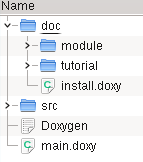
\includegraphics[width=0.4\textwidth]{image/doc-struct}
    \caption[ساختار مورد نیاز برای ایجاد مستند تکنیکی]
    {
      ساختار مورد نیاز برای یک مستند تکنیکی. هماگونه که در این تصویر قابل مشاهده
      است یک مسیر به نام \lr{doc} ایجاد می‌شود و مستندهای جانبی در آن قرار
      می‌گیرد. دیگر مستندها در متن برنامه نوشته می‌شود.
    }
    \label{standard/where-what/doc-struct}
  \end{figure}


%
% حق نشر 1390-1402 دانش پژوهان ققنوس
% حقوق این اثر محفوظ است.
% 
% استفاده مجدد از متن و یا نتایج این اثر در هر شکل غیر قانونی است مگر اینکه متن حق
% نشر بالا در ابتدای تمامی مستندهای و یا برنامه‌های به دست آمده از این اثر
% بازنویسی شود. این کار باید برای تمامی مستندها، متنهای تبلیغاتی برنامه‌های
% کاربردی و سایر مواردی که از این اثر به دست می‌آید مندرج شده و در قسمت تقدیر از
% صاحب این اثر نام برده شود.
% 
% نام گروه دانش پژوهان ققنوس ممکن است در محصولات دست آمده شده از این اثر درج
% نشود که در این حالت با مطالبی که در بالا اورده شده در تضاد نیست. برای اطلاع
% بیشتر در مورد حق نشر آدرس زیر مراجعه کنید:
% 
% http://dpq.co.ir/licence
%
\section{پیکره بندی}
در این قسمت به بررسی پرونده پیکر بندی مورد نیاز برای ایجاد مستن خواهیم پرداخت
در این پرونده علاوه بر این که تنظیمات اولیه مورد نیاز برای ایجاد مستند وجود
دارد چگونگی ایجاد مستند نیز به صورت کامل تشریح می‌شود. همواره فرض می‌شود که هر
پروژه یا قطعه در یک پروژه به صورت کامل در یک پوشه هم نام با آن قرار دارد. تمام
قطعه‌ها و پروژه‌هایی که با هم دیگر یک پروژه کلی را ایجاد می‌کنند نیز کنار یک
دیگر و در یک پوشه قرار می‌گیرند.

مستند تکنیکی ایجاد شده از سیستم نیز خود یک زیر پروژه از پروژه کلی در نظر گرفته
می‌شود از این رو باید یک پوشه، در پوشه پروژه اصلی در نظر گرفت. این پوشه را
همواره با نام \lr{doc} در نظر می‌گیریم. مستند تکنیکی هر زیر پروژه باید به صورت
یک پرونده هم نام با همان زیر پروژه در پوشه \lr{doc} ایجاد شود. برای نمونه فرض
کنید که در پروژه اصلی سه زیر پروژه به نام‌های \lr{GUI}، \lr{Shell} و \lr{LIB}
وجود دارد. در این صورت در این پروژه یک پوشه دیگر به نام \lr{doc} باید ایجاد
و معادل با هر زیر پروژه در آن یک پوشه ایجاد شود. در شکل
\ref{wher-what-config-example-1} ساختار مورد نیاز برای این پروژه نمایش داده
شده است.

در گام بعد در هر پروژه یک پرونده پیکره بندی برای مستند فنی به نام \lr{Doxygen}
ایجاد می‌شود که داده‌های مورد نیاز برای ایجاد مستند در آن قرار خواهد گرفت. در
شکل \ref{wher-what-config-example-1} محل قرار گرفتن پرونده‌های پیکره بندی نشان
داده شده است. از آنجا که محل خروجی مستندهای ایجاد شده بر اساس تنظیم‌های موجود
در همین پرونده‌های تعیین می‌شود باید خصوصیت مسیر خروجی برای هر مستند را به
گونه‌ای اصلاح کرد که مستندهای ایجاد شده در مسیر مناسب قرار گیرد. برای نمون در
پرونده پیکربندی پروژه \lr{GUI} مسیر خروجی به صورت زیر اصلاح می‌شود:

\begin{latin}
\lstset{language=bash}  
\begin{lstlisting}[frame=single] 
OUTPUT_DIRECTORY       = ../doc/GUI
INPUT                  = ./
\end{lstlisting}
\end{latin}

همانگونه که در نمونه آورده شده قابل مشاهده است علاوه بر مسیر خروجی باید مسیر
ورودی پروژه را نیز تعیین کرد. از آنجا که برای هر پروژه به صورت جداگانه یک پرونده
پیکره بندی ایجاد می‌شود کافی است که مسیر ورودی را مسیر جاری قرار داد. با این
تنظیم بدون ترس از محل قرار گرفتن مستند‌ها می‌توان به سادگی در پایان پروژه مستند
فنی را بر اساس تمام پروژه‌ها موجود در پروژه اصلی ایجاد کرد. این فرآیند می‌تواند
به صورت خودکار در پروژه‌های بزرگ انجام شود.

مستندگر \lr{Doxygen} تنها مسیر ورودی تعیین شده را برای یافتن پرونده‌های ورودی
جستجو می‌کند، در صورتی که ساختار تشریح شده برای مستندها و برنامه‌ها به صورت
سلسله مراتبی در نظر گرفته شده است. در این حالت در پرونده پیکره بندی باید جستجوی
بازگشتی برای یافتن پرونده‌ها فعال شود. برای فعال کردن این روش جستجو باید تنظیم
زیر را در پرونده پیکره بندی اضافه کرد:

\begin{latin}
\lstset{language=bash}  
\begin{lstlisting}[frame=single] 
FILE_PATTERNS          = *.h \
                         *.hh \
                         *.hxx \
                         *.hpp \
                         *.h++ \
                         *.dox \
                         *.doxy

RECURSIVE              = YES
\end{lstlisting}
\end{latin}

همانگونه که در کده بالا قابل مشاهده است علاوه بر فعال کردن جستجوی بازگشتی،
می‌بایست ساختارها و پرونده‌هایی که باید به عنوان ورودی قرار گیرد را تعیین کرد.
گرچه که پرونده‌های ورودی وابسته بر اساس نوع پروژه و زبان‌های برنامه سازی به کار
گرفته شده در آن تعیین می‌شود، اما در هر حال پرونده‌های با پسونده \lr{*.doxy}
باید همواره به عنوان ورودی مورد استفاده قرار گیرد.

علاوه بر تمام خصوصیت‌هایی که در این بخش مورد بررسی قرار گرفت خصوصیت‌های دیگری
نیز وجود دارد که باید در یک پرونده پیکرده بندی تعیین شوند. در کد زیر  برخی از
مهم‌ترین تنظیم‌های مورد نیاز برای یک پروزه آورده شده است:

\begin{latin}
\lstset{language=bash}  
\begin{lstlisting}[frame=single] 
DOXYFILE_ENCODING      = UTF-8
PROJECT_NAME           = My Project GUI
PROJECT_NUMBER         = 0.1.0 beta
PROJECT_BRIEF          = MGUI
PROJECT_LOGO           = ./images/logo.png
\end{lstlisting}
\end{latin}

در نهایت با ایجاد تنظیم‌های مورد نیاز برای تمام پروژه‌ها می‌توان به سادگی مستند
فنی مورد نیاز برای پروژه را ایجاد و در موقع نیاز از آنها استفاده کرد.

%
% حق نشر 1390-1402 دانش پژوهان ققنوس
% حقوق این اثر محفوظ است.
% 
% استفاده مجدد از متن و یا نتایج این اثر در هر شکل غیر قانونی است مگر اینکه متن حق
% نشر بالا در ابتدای تمامی مستندهای و یا برنامه‌های به دست آمده از این اثر
% بازنویسی شود. این کار باید برای تمامی مستندها، متنهای تبلیغاتی برنامه‌های
% کاربردی و سایر مواردی که از این اثر به دست می‌آید مندرج شده و در قسمت تقدیر از
% صاحب این اثر نام برده شود.
% 
% نام گروه دانش پژوهان ققنوس ممکن است در محصولات دست آمده شده از این اثر درج
% نشود که در این حالت با مطالبی که در بالا اورده شده در تضاد نیست. برای اطلاع
% بیشتر در مورد حق نشر آدرس زیر مراجعه کنید:
% 
% http://dpq.co.ir/licence
%
\section{برگه نخست}
  برگه نخست ابتدایی ترین قسمت در یک مستند است، از این جهت در ایجاد و سازمان دهی
  یک مستند بسیار مهم است.
  اگر این صفحه به درستی و به شیوه مناسب طراحی و ایجاد نشده باشد، خواننده مستند
  نمی‌تواند به سادگی مستند را مور استفاده قرار دهد و در نخستین برخورد دچاد
  سردرگمی خواهد شد.

  پیش از هر چیز باید به این نکته اشاره کرد که برگه عبارت است از یک بخش از مستند
  که در حالت کلی معادل با یک گفتار در یک کتاب است.
  هر برگه را در یک پرونده \lr{*.doxy} ایجاد می‌شود و در آن متن برگه به صورت کامل
  نوشته می‌شود.
  هر برگه همانند یک گفتار می‌تواند از بخشهای متفاوتی ایجاد شده باشد.
  هر بخش و زیر بخشهای آن نیز به صورت منظم و پشت سرم هم در پرونده برگه نوشته
  می‌شود. در کد زیر نمونه‌ای از یک برگه آورده شده است.
  
\begin{latin}
\lstset{language=C++}
\begin{lstlisting}[frame=single] 
/**
\page pageid Page Title
  Page Body.
  
  \section sectionid Section Title
    Section Body.

    \subsection subsectionid Subsection Title
      Subsection Body.
*/
\end{lstlisting}
\end{latin}

  همانگونه گه پیش از این نیز گفته شد، برگه نخست ابتدایی ترین قسمتی از مستند است
  که هر خواننده با آن روبرو می‌شود. بی شک انتخاب دقیق مطالب مورد نیاز و
  ساختاردهی آن در تاثیر پذیری آن اثر خواهد داشت.
  در نخستین قسمت از برگه نخست باید به معرفی نرم افزار و بیان اهداف اصلی طراحی و
  ایجاد آن اختصاص داده شود.
  هر خواننده با دانستن اهداف یک نرم‌افزار یا بسته نرم‌افزاری می‌تواند به چرایی
  بسیاری از رویکردهای سیستم پاسخ دهد.
  دور از ذهن نیست که برای انجام هر پردازش ویا اجرای هر فرآیند در یک سیستم
  نرم‌افزاری روش‌های متفاوتی وجود داشته باشد. برای نمونه در ذخیره و بازیابی
  داده‌های می‌توان از روش‌های متفاوتی چو پایگاه داده‌ها، پرونده‌های متنی و
  باینری و یا بسیاری از روش‌های دیگر استفاده کرد. واضح است که خواننده با اشراف
  بر اهداف یک سیستم می‌تواند به راحتی درک کند که چرا در یک مسئله از روشی خاص
  استفاده شده است و در نتیجه توانایی و محدودیت سیستم در کجا است.

  در توسعه یک سیستم مدیران پروژه در نخستین گام به دنبال سیستم‌های موجودی خواهند
  بود که بتواند تمام اهداف مورد نظر آنها را پوشش دهد. در بسیاری از موارد نیز
  اهداف و نیازهای سیستم مورد بازبینی قرار گرفته و گه گاه از آنها کاسته می‌شود تا
  کاملا با اهداف یک سیستم موجود هم سو شود. در این صورت ابتدایی ترین پرسش مطرح
  برای یک مدیر اهداف یک سیستم ایجاد شده است. بر این اساس ایجاد یک بخش مجزا و
  تشریح اهداف یک سیستم بسیار اساسی به نظر می‌رسد.

  شکی نیست که پیش از هرچیز در یک مستند تکنیکی باید سیستم را به صورت کامل تعریف
  کرد و اهداف مورد نظر در طراحی و پیاده سازی آن را تشریح کرد اما علاوه بر این
  نیاز است که ساختار مستند نیز به صورت کامل تشریح شود. این تصور اشتبا است که
  همواره هر خواننده از ابتدایی ترین موضوع در مستند شروع کرده و تا انتها تمام
  ستند را به ترتیب مطالعه خواهد کرد.
  خوانندگان یک مستند با دیدگاهی متفاوت تنها به دنبال دسته‌ای خاص از اطلاعات
  ایجاد شده در یک مستند هستند و از خواندن بسیار از بخشهای مستند صرف نظر خواهند
  کرد. در این حالت معرفی مفید و کامل ساختار مستند می‌تواند بسیار مفید واقع شود و
  احساس خوبی را در خوانندگانی که برای اولین بار مستند را مطالعه می‌کنند ایجاد
  کند.

  مدیران  سیستم‌های نرم افزاری در فرآیند گزینش یک سیستم جدید در پی داده‌های چون
  سخت‌افزارهای مورد نیاز، وابستگی به بسته‌های نرم‌افزاری دیگر، قابلیت انتقال به
  روی سکوی‌های متفاوت و دیگر اطلاعات از یک سیستم موجود هستند. این در حالی است که
  توسعه دهندگان سیستم‌های نرم افزاری بیشت به دنبال اطلاعاتی در زمینه به کار گیری
  سیستم در کاربردهای مورد نظر هستند. اینها تنها بخشی از خوانندگان با دیدهای
  متفاوت هستند که مستند تکنیکی سیستم‌های موجود را مورد بررسی و مطالعه قرار
  می‌دهد. در چنین شرایطی ایجاد ساختار مناسب در مستندها و تشریح کافی و کامل آن
  می‌تواند خوانندگان را در یافتن اطلاعات مورد نظرشان از یک سیستم موجود یاری کند.

  سومین بخش از برگه نخست مستند که باید در نظر گرفته شود، بیان سطوح متفاوت موجود
  در یک مستند و توصیه‌های مناسب برای خوانندگان مستند است. بی شک مستند یک سیستم،
  به خصوص زمانی که اندازه سیستم بزرگ است، زمینه‌های متفاوتی را پوشش داده و در
  نتیجه خوانندگان متفاوتی را به خود خواهد دید از این رو تعیین زمینه‌های متفاوت
  موجود و توصیه مناسب به خوانندگانی که قصد مطالعه مستند را دارند می‌تواند آنها
  را در یافتن مناسب اطلاعات مورد نیازشان یاری کند. در کد نمونه‌ای که در ادامه
  آورده شده است یک ساختار ابتدایی برای برگه نخست مستند ارائه شده است.
\begin{latin}
\lstset{language=C++}
\begin{lstlisting}[frame=single] 
/**
\mainpage
  Introduction

\section docstruct Document Structuer
  Document Struction

\subsection whoread Who Read
  Who Read

\section whatsnew New
  What is New

\section bugs Closed Bugs
  Bugs
*/
\end{lstlisting}
\end{latin}

  همان گونه که در متن مستند نوشته شده قابل مشاهد است، دو بخش جدید نیز در انتهای
  برگه نخست پیش بینی شده است.
  اولین بخش در مورد توانایی‌های جدیدی است که به نسخه جدید از سیستم اضافه شده است
  در حالی که دومین بخش در مورد خطا‌هایی است که از نسخه پیشین حذف شده است. این دو
  بخش در رابطه با سیستم‌هایی است که دورده زمانی زیادی را دارند و در نسخه‌های
  متفاوت توسعه می‌یابند.

  
%
% حق نشر 1390-1402 دانش پژوهان ققنوس
% حقوق این اثر محفوظ است.
% 
% استفاده مجدد از متن و یا نتایج این اثر در هر شکل غیر قانونی است مگر اینکه متن حق
% نشر بالا در ابتدای تمامی مستندهای و یا برنامه‌های به دست آمده از این اثر
% بازنویسی شود. این کار باید برای تمامی مستندها، متنهای تبلیغاتی برنامه‌های
% کاربردی و سایر مواردی که از این اثر به دست می‌آید مندرج شده و در قسمت تقدیر از
% صاحب این اثر نام برده شود.
% 
% نام گروه دانش پژوهان ققنوس ممکن است در محصولات دست آمده شده از این اثر درج
% نشود که در این حالت با مطالبی که در بالا اورده شده در تضاد نیست. برای اطلاع
% بیشتر در مورد حق نشر آدرس زیر مراجعه کنید:
% 
% http://dpq.co.ir/licence
%
\section{برگه‌های دیگر}
  علاوه بر برگه نخست برگه‌های دیگری نیز در مستند وجود دارند که جنبه‌های متفاوتی
  از سیستم را مورد بررسی قرار می‌دهند. نصب و راه اندازی، مبانی مورد استفاده در
  سیستم، به کارگیری و خطاهای متداول سیستم تنها بخشی از مستندهایی است که معمولا
  در یک مستند تکنیکی وجود دارد.

  به این نکته باید توجه داشت که در یک مستند تکنیکی دو جنبه کاملا مجزا و در عین حال
  تاثیر گذار وجود دارد: ساختار و سازماندهی مستندها. ساختار
  مستند (همانگونه که در بخش پیش به آن اشاره شد) به چینش و ترتیب مستندهای ظاهر
  شده در متن مستند گفته می‌شود. بخش‌ها زیر بخش‌ها گفتارها و جنبه‌هایی از سیستم که باید 
  مور بررسی قرار گیرد همگی موضوعاتی هستند که در ساختار دهی مستند مورد توجه قرار می‌گیرند.
 این درحالی است که سازمان
  دهی مستند فرآیندی است که در آن قرار دادن مستندها در مسیرهای مشخص، تعیین نام پرونده‌ها و مدیریت
  مستند ایجاد شده پرداخته می‌شود.

  برای نمونه این که تمام مستندهای جانبی باید در مسیر \lr{doc} قرار گیرد و با پسوند
  \lr{*.doxy} ذخیره شود به سازماندهی مستند است در حالی که معرفی سیستم و
  تشریح اهداف آن به ساختار مستند مربوط می‌شود.
  در طراحی مستند مناسب باید به هر دو جنبه مورد توجه باشد، از این رو در این بخش هر دو
  جنبه مورد بررسی قرار خواهد گرفت. از انجا که تعیین یک مرز کاملا مشخص بین این
  دو دشوار و در برخی موارد منجر به پیچیده شدن موضوع می‌شود هر دو آنها باهم مورد بررسی قرار خواهد گرفت.

  هر برگه معادل با یک فصل در نظر گرفته خواهد شد که در یک پرونده جدا با پشوند
  \lr{*.doxy} ایجاد می‌شود. از این رو برگه‌ها نیز باید در مسیر دیگر مستندهای
  جانبی یعنی در پوشه \lr{doc} قرار بگیرند.
  هر بخش با استفاده از برچسب \lr{page} در مستند مشخص شده که با استفاده از یک
  شناسه در کل مستند قابل آدرس دهی است.
  از آنجا که شناسه هر برگه منحصر به فرد است، استفاده از شناسه برگه به عنوان نام
  پرونده نه تنها مشکل نام گذاری پرونده‌ها را حل می‌کند بلکه منجر به دستیابی راحت
  به برگه‌ها در زمان توسعه مستند می‌شود. با این روش به سادگی و تنها با مشاهده
  نام پرونده می‌توان از مطالب درون آن اطلاع یافت.

  یک برگه می‌تواند به عنوان یک زیر بخش و یک زیر برگه از یک برگه دیگر در نظر
  گرفته شود (اضافه کردن یک برگه به عنوان زیربرگ در برگه دیگر با استفاده از برچسب
  \lr{subpage} انجام می‌شود که شرح کامل آن در بخش بسته بندی مستند آمده است).

  زمانی که تعداد زیربرگه‌های یک برگه زیاد می‌شود بهتر است که آنها را در یک پوشه
  جدا ( و هم نام با شناسه برگه) قرار داد. اما اگر تعداد زیر برگه‌ها کم باشد
  می‌توان آنها را در انتهای پرونده برگه اصلی اضافه کرد. مستند زیر یک نمونه از
  ایجاد برگه و زیر برگه‌ها در یک پرونده را نشان می‌دهد.

\begin{latin}
\lstset{language=C++}
\begin{lstlisting}[frame=single]
/**
\page pageid Example
  Page budy
  ....
  \subpage subpageid1
  \subpage subpageid2
  ....
*/
/**
\page subpageid1 Subpage Title 1
...
*/
....
\end{lstlisting}
\end{latin}

  مناسب ترین روش، ایجاد برگه‌های اصلی در مسیر \lr{doc} و ایجاد زیر برگه‌ها هر یک در زیر
  پوشه‌های مجزا به ازای هر برگه اصلی است - برگه اصلی در اینجا به معنی برگه‌هایی
  است که به عنوان زیر برگ هیچ برگ دیگر از مستند نباشد.

  تعیین برگه‌های اصلی مورد نیاز در هر مستند دشوار است و بسته به اندازه و نوع
  پروژه می‌تواند بسیار متفاوت باشد. اما دسته‌ای از این برگه‌ها
  تقریبا در تمام مستندهای تکنیکی وجود دارند.
  در فهرست زیر پر کاربرد ترین برگه‌های موجود در مستندهای تکنیکی آورده شده است:
  \begin{itemize}
   \item نصب و راه اندازی
   \item مبانی
   \item کاربردها
   \item پرسشهای متداول
  \end{itemize}
  در ادامه این بخش، این برگه‌ها به صورت مفصل‌تر مورد بررسی قرار  خواهد گرفت.

  
  
\subsection{نصب و راه اندازی}
  راهنمای نصب یک نرم‌افزار در بسیاری از موارد با راهنمای مدیریت و کاربری یک
  سیستم نرم افزاری و یا سخت افزاری هم پوشانی دارد. این هم پوشانی به دلیل وجود
  تنظیم‌های مورد نیاز در فرآیند نصب است که به عنوان حالت اولیه سیستم در نظر
  گرفته می‌شود.

  نصب و راه اندازی سیستم با تنظیم و به کارگیری آن در رابطه است و
  گاه شامل اطلاعاتی می‌شود که در مستندهای دیگر مانند مستند مدیریت و یا کاربری 
  هم پوشانی دارد. در این شرایط مناسب است که به مستندهای دیگر ارجاع داده شده و از
  ذکر دوباره اطلاعات خوداری کرد. اما باید به این نکته توجه داشت که بیان دوباره
  نکته‌های مهم می‌تواند در مستقل شدن مستند و نصب سریع و آسان سیستم کمک کند. به
  هر حال نباید از زیاده گویی و افزونگی مستند غافل شد.

  موارد متفاوتی وجود دارد که در این بخش باید به صورت کامل به آن پرداخته شود. در
  اینجا برخی از موارد لاز در فرآیند نصب و راه اندازی سیستم بیان و 
روش مستندسازی آنها مورد بررسی قرار گرفته شده است.


\paragraph{پیش نیازها}
   چه نوع نرم‌افزار، سخت افزار، و یا سکوی نرم‌افزاری برای نصب یک سیستم مورد نیاز
   است؟ آیا سیستم به روی هر سکوی نرم افزاری و یا سخت افزاری قابل اجرا است؟ آیا
   سیستم با سیستم‌های عامل متفاوت چون لینوکس، مک، و یا ویندوز سازگار است؟
   پردازشگر مورد نیاز سیستم چه قابلیت‌هایی باید داشته باشد؟ اینها بخشی از
   پرسش‌هایی است که باید در این بخش به آن پرداخته شود.

   توجه به این نکته بسیار مهم است که پیش‌نیازهای یک سیستم گاهی از خود آن نیز
   مهم‌تر می‌شود. برای نمونه حالتی را تصور کنید که در آن سیستم به صورتی ایجاد
   شده است که تنها به روی یک سیستم عامل خاص قابل اجرا است در این صورت فرد یا
   گروهی که به آن سیستم عامل دسترسی ندارند نمی‌توانند از این سیستم استفاده کنند.
   پیش‌نیازهای یک سیستم در انتخاب یک سیستم بسیار موثر خواهد بود.

   به عنوان نمونه در راهنمای نصب سیستم عامل ویندوز ویستا، موارد زیر به عنوان
   پیش‌نیاز نصب سیستم معرفی شده است:
\begin{config}
1 GHz 32-bit (x86) or 64-bit (x64) processor
512 MB of system memory
20 GB hard drive with at least 15 GB of available space
Support for DirectX 9 graphics and 32 MB of graphics memory
DVD-ROM drive
Audio Output
Internet access
\end{config}
   بر اساس این پیش‌نیازها کاربران و مدیران می‌توانند سیستم مورد نیاز
   خود را بر اساس پیش‌نیاز آنها انتخاب کنند. گرچه یک سیستم ایده آل سیستمی است که پیش‌نیازهای آن کم و
   با هر شرایطی سازگار باشد اما در هر حال باید پیش‌نیاز سیستم به درستی تعیین شده
   باشد تا کاربران در فرآیند نصب و راه اندازی سیستم با مشکل روبرو نشوند.
   
\paragraph{دست یابی به سیستم}
  پیش از هر کاری نیاز است که کاربران به نرم‌افزار و یا کد منبع آن دست پیدا کنند.
  در این بخش بر اساس توافق نامه یک نرم‌افزار به کاربران اطلات لازم جهت دست یابی
  که نرم افزار داده می‌شود. برای نمونه در سیستم های متن باز به کاربران آموزش
  داده می‌شود که چگونه با استفاده از مدیریت نسخه‌ها به یک نسخه خاص از کد منبع
  نرم‌افزار دست پیدا کنند.
  
\paragraph{تنظیم و نصب سریع}
   گاهی در مستند‌های فنی از این بخش به عنوان شروع سریع یاد می‌کنند که در آن
   فرآیند نصب و به کارگیری عملی سیستم با کمترین تنظیم و منابع تشریح می‌شود. به
   کارگیری ساده و سریع یک سیستم می‌تواند اعتماد کاربران را به سیستم افزایش دهد.

   در این بخش پیش شرط‌های مورد نیاز برای نصب، حالت نرم‌افزار و سخت‌افزارهای مورد
   استفاده و درک لازم از حالت سیستم به صورت کامل تشریح شده و کاربر برای نصب
   مقدماتی سیستم آماده می‌شود. علاوه بر این در این بخش عبارت‌ها و واژگان جدید
   مطرح در سیستم که حالت و یا قسمت خاصی از سیستم را تشریح می‌کند به صورت کامل
   بیان می‌شود.

   روش مناسب برای تعیین درک کامل از سیستم، تشریح سیستم و ساختار آن با
   استفاده از نمودارها است.
   ساختار سیستم، واسطه‌های مورد حمایت، شبکه‌های مورد استفاده و بسیاری دیگر از
   اجزای مورد نیاز سیستم را می‌توان با استفاده از یک نمودار به سادگی تشریح
   کرد و درک کاملی را از سیستم و پیش‌نیازهای آن به وجود آورد. درک سیستم نه تنها
   فرآیند نصب را قابل درک کرده بلکه کاربران را در تعیین و رفع مشکلات سیستم یاری
   می‌کند. در شکل 
   \ref{تصویر-ساختار-خوشه-پایگاه-داده}
    یک نمونه از شکل‌های مورد
   استفاده در راهنمای نصب یک سیستم نرم‌افزاری نمایش داده شده است.
  \begin{figure}
    \centering
    \includegraphics[width=0.75\textwidth]{image/mysql-cluster-install.png}
    \caption[ساختار خوشه‌ای پایگاه داده]
    {
      در این تصویر ساختار خوشه‌ای \lr{MySQL} نمایش داده شده است. بر اساس این
      ساختار کاربران می‌توانند پیش نیازهای سیستم را در نصب خوشه‌ای و تفاوت آن را
      با دیگر روش‌های نصب در این نرم افزار درک کند.
      از این شکل در راهنمای نصب این نرم‌افزار استفاده شده است.
    }
    \label{تصویر-ساختار-خوشه-پایگاه-داده}
  \end{figure}
  
   کاربران سیستم در اولین برخورد و مبتنی بر مستندهای این بخش است که قادر خواهند بود
   سیستم را به صورت عملی نصب کرده و به کار ببرند. لذا طراحی و نوشتن مناسب این بخش
   می‌تواند در جلب اعتماد کاربران بسیار مفید باشد. به این نکته توجه داشته باشید
   که زمانی یک کاربر به سیستم اعتماد کند آن را به کار خواهد بست و در ادامه
   تنظیم‌های پیشرفته سیستم را نیز فرا خواهد گرفت. پژوهشها نشان می‌دهد که عدم
   توانایی نصب راحت و به کار گیری یک سیستم منجر به کاهش علاقه کاربران در به
   کارگیری سیستم خواهد شد از این رو پرداختن به این بخش می‌تواند بسیار مهم باشد.

\paragraph{آزمون و خطایابی}
    تمام سیستم‌های نرم‌افزاری و سخت‌افزاری از روش‌های متفاوتی برای نمایش حالت
    درونی سیستم استفاده می‌کنند.
    واسطه‌ها گرافیکی، پیام‌های صوتی تصویری، دریچه‌های محاوره‌ای بخشی از روکردهای
    مورد استفاده در نمایش حالت درونی یک سیستم نرم‌افزاری است. سیستم‌های
    نرم‌افزاری با استفاده از همین رویکردها رویدادهای داخلی سیستم را به
    کاربران گزارش می‌کنند.

    در این بخش باید به صورت کامل به خطاهای احتمالی در فرآیند نصب یک نرم‌افزار
    پرداخته شده و راه مناسب رفع آنها به صورت کامل تشریح شود. اطلاعات موجود در
    این بخش می‌تواند کاربران را در نصب و راه‌اندازی راحت سیستم یاری کند.

    برای نمونه فرض کنید که سیستمی فیزیکی وجود دارد و در جلو آن چراغی با چهار
    رنگ قرار تعبیه شده است.
    این سیستم با استفاده از رنگهای متفاوت این چراغ‌ها حالت درونی خود را به کاربران
    سیستم گزارش می‌کند.
    از این رو در این بخش از مستند به تشریح مفهوم رنگ‌های متفاوت و روش برخورد با هر 
یک بیان می‌شود. برای نمون چراغ قرمز به معنی مناسب نبودن
    منبع تغذیه است که در این صورت باید سیستم خاموش شده و منبع تغذه آن تعمیر شود.

    تشریح روش‌های مناسب آزمون سیستم بعد از نصب نیز یکی دیگر موضوعاتی است که در
    این بخش به آن پرداخته می‌شود. اطمینان از نصب بودن و درستی حالت درونی یک
    سیستم برای استفاده عملی از آن بسیار اساسی است.

\paragraph{به روز رسانی}
    علاوبه بر نصب یک سیستم نرم‌افزاری به روز رسانی آن نیز از اهمیت زیادی
    برخوردار است. کاربران باید به صورت کامل از فرآیند به روز رسانی سیستم آگاه
    بوده و بتواند سیستم را به روز کند.

    محدودیت‌های به روز رسانی و یا توافق نامه‌های مورد نیاز در به روز رسانی
    باید در این بخش مورد بررسی قرار گیرد. کاربران بر اساس این توافق نامه
    می‌توانند در مورد استفاده یا عدم استفاده از یک بسته نرم‌افزاری تصمیم بگیرند.
    
\subsection{مبانی}

مبانی در اینجا، آن دسته از دانش‌های فنی است که نرم‌افزار مبتنی بر آنها توسعه یافته است.
برای نمونه می‌توان بسته‌های متفاوتی نام برد که بر اساس مبانی خاص ریاضی توسعه یافته‌اند
و در کاربردهای خاص مورد استفاده قرار می‌گیرند. مبانی مورد استفاده باید به صورت کامل و روشن
بیان شود تا نه تنها توسط تیم توسعه در آیند، بلکه کاربران سیستم مورد استفاده قرار گیرد.

حجم مستند مبانی ممکن است از یک صفحه تا چندین بخش قابل متغییر باشد، اما نکته‌ای که باید در نوشتن
مبانی مورد توجه قرار گیرد بیان کامل و روشن تمام مبانی مورد استفاده است. این نکته به ویژه زمانی
که نظریه‌های متفاوتی در راستای اهداف پروژه وجود دارد و تمییز بین این نظریه‌ها از اهمیت
ویژه‌ای برخوردار است، پر اهمیت می‌شود.
  
\subsection{کاربردها}
بی شک هر سیستم بر اساس اهداف از پیش تعریف شده‌ای سازمان دهی و پیاده‌سازی می‌شود. اهداف سیستم 
در بسیاری از موارد منجر به ایجاد بسیاری از محدودیت‌ها در سیستم پیاده‌سازی شده خواهد شد، از این
رو لازم است که نه تنها تمام کاربردهای نرم‌افزار بلکه محدودیت‌های آن نیز به صورت کامل بیان شود.
در این بخش تمام کاربردهای و محدودیت‌های سیستم بیان و به صورت کامل مورد بررسی قرار خواهد گرفت.
  
\subsection{پرسشهای متداول}
نمی‌توان تصور کرد که مستند ایجاد شده برای یک سیستم به صورت کامل واضح و کامل است. بسیاری از کاربران
طی استفاده از سیستم‌ها با پرسش‌های روبرو می‌شوند که به خوبی می‌تواند کاستی‌های مستندهای موجود را بیان 
می‌کند. در این برگه متداول‌ترین پرسش‌های مطرح در بین کاربران تعیین و به صورت کامل پاسخ داده می‌شود
تا به واضح‌تر شدن مستند فنی و کاربردهای نرم‌افزار بیفزاید.
  
\subsection{پیمان نامه‌ها}
مهم‌ترین قسمت یک مستند فنی، پیمان‌نامه آن است. در این قسمت از مستند به صورت کامل محدودیت‌های نرم‌افزار
ایجاد شده از نظر حقوقی بیان می‌شود که در انتخاب و به کارگیری هر سیستمی مهم است. گروه‌های متفاوت
از پیمان نامه‌های متفاوت استقبال و نرم‌افزارهای مورد نیاز خود را بر اساس همین پیمان نامه‌ها 
انتخاب می‌کنند.
  


%
% حق نشر 1390-1402 دانش پژوهان ققنوس
% حقوق این اثر محفوظ است.
% 
% استفاده مجدد از متن و یا نتایج این اثر در هر شکل غیر قانونی است مگر اینکه متن حق
% نشر بالا در ابتدای تمامی مستندهای و یا برنامه‌های به دست آمده از این اثر
% بازنویسی شود. این کار باید برای تمامی مستندها، متنهای تبلیغاتی برنامه‌های
% کاربردی و سایر مواردی که از این اثر به دست می‌آید مندرج شده و در قسمت تقدیر از
% صاحب این اثر نام برده شود.
% 
% نام گروه دانش پژوهان ققنوس ممکن است در محصولات دست آمده شده از این اثر درج
% نشود که در این حالت با مطالبی که در بالا اورده شده در تضاد نیست. برای اطلاع
% بیشتر در مورد حق نشر آدرس زیر مراجعه کنید:
% 
% http://dpq.co.ir/licence
%
\section{مستند پیاده سازیی}
همان گونه که پیش از نیز بیان شد، علاوه بر مستند فنی دسته‌ای دیگر از مستندها وجود دارد که در مورد 
پیاده سازی سیستم است. در این مستند برخلاف مستند فنی به روش مورد استفاده در پیاده سازی متدها و 
الگوریتم‌ها ذکر می‌شود تنها در توسعه سیستم مورد استفاده است. گرچه مستند پیاده سازی از اهمیت ویژه‌ای
برخوردار است، با این وحود نباید در مستند فنی ظاهر شود.

فرض کنید که یک توسعه دهنده سیستم در زمان پیاده سازی به یک ایده جدید در مورد پیاده سازی سیستم 
رسید است. این ایده یک مستند بسیار مهم است که باید در سیستم نگه داشته شود (تا جایی که بسیاری
از متدلوژی‌ها بر اساس این ایده‌ها سازمان‌دهی می‌شوند). مستندهای از این دست، کاملا در مورد پیاده‌سازی
سیستم است از این رو کاربردی برای کاربران سیستم ندارند.

مستندهای پیاده سازی در لابلای کدها نوشته می‌شود و از ساختار سازمان یافته‌ای همانند مستند فنی برخوردار
نیستند. گرچه چگونگی نوشتن مستند پیاده سازی کاملا شخصی است با این وجود دسته‌ای از استاندارهای برای سازمان
دهی آن وچود دارد که در ادامه به آن پرداخته خواهد شد.
مستند پیاده سازی به دو روش در برنامه‌ها بیان می‌شود: چند و تک خطی. زمانی که مستند پیاده سازی طولانی
است به صورت چند خط نوشته می‌شود این مستند به صورد زیر نوشته می‌شود:
 
\begin{latin}
\lstset{language=C++}
\begin{lstlisting}[frame=single] 
/*
 * Implementation document
 * this document is structed in multi line.
 */
\end{lstlisting}
\end{latin}

البته مستندهای کوتاه تنها در یک خط و به صورت زیر در متن برنامه‌ها نوشته می‌شود:

\begin{latin}
\lstset{language=C++}
\begin{lstlisting}[frame=single] 
// Implemtnation Doceumtn
\end{lstlisting}
\end{latin}

هر قسمت مستند که به صورت یکی از دو روش بالا در متن برنامه‌ها نوشته شود به عنوان یک مستند پیاده سازی
در نظر گرفت شده و در مستند فنی تولید شده وارد نخواهد شد.

\subsection{برچسب‌های مستند پیاده‌سازی}
فرض کنید که یک گروه پیاده‌سازی می‌خواهد با استفاده از یک ماشین برنامه ایجاد شده را به صورد کامل
بررس کرده و بر اساس آن پیام‌های مناسبی را در جهت بهبود و گسترش سیستم، ایجاد کند. بی شک این ماشین
باید مستندهای پیاده سازی را بررسی کرده و پیام‌های خود را مبتنی بر آنها ایجاد کند. برای نمونه انتظار
می‌رود که برنامه تعیین کند که کدام قسمت‌ها از برنامه ایجاد شده نیاز به بازنویسی، بهبود و یا حذف شدن 
دارد تا بتواند در فرآیند توسعه مورد استفاده قرار گیرد. بی شک این ماشین بدون در نظر گرفتن استاندارهای
مناسب برای نوشتن مستند پیاده سازی نمی‌تواند پیام‌های مناسبی را ایجاد کند. در این قسمت یک ساختار ابتدایی
برای نوشتن مستند پیاده سازی تشریح خواهد شد که می‌تواند این فرآیند را به صورت کامل پوشش دهد.

برخلاف مستند فنی، در مستند پیاده‌سازی تنها تعداد محدودی برچسب موجود است که برای ساختاردهی مستند مورد
استفاده قرار می‌گیرد. این برچسب‌ها باید هموار در ابتدای نخستن خط از هر بسته مستند پیاده سازی نوشته
شده و به صورت کامل از ساختار تعریف شده پیروی کند. گرچه امکان نوشتن مستند پیاده‌سازی در چندین خط وجود
دارد اما همواره در سطر اول باید با استفاده از یک جمله به صورت کامل و شفاف هدف اصلی مستند نوشته شود.
علاوه بر این باید تعیین شود که چه فردی و در چه زمان مستند را ایجاد و یا ویرایش کرده است. مستند زیر
را در نظر بگیرد:


\begin{latin}
\lstset{language=C++}
\begin{lstlisting}[frame=single] 
/*
 * TODO : maso 1390-12 : Document title.
 * document text.
 */
\end{lstlisting}
\end{latin}

همان گونه که در این قطعه مستند قابل مشاهد است، در سطر نخست با استفاده از یک برچسب، نام توسعه دهنده، 
تاریخ و عنوان نه تنها مفاهیم کلی مستند انتقال یافته بلکه امکان ردیابی اطلاعات نیز ممکن شده است. 
برای سادگی و ایجاد تمایز میان برچسب‌های مورد استفاده در مستند فنی و پیاده سازی، برچسب‌های مورد استفاده
در مستند پیاده‌سازی را چمپ\LTRfootnote{برچسب مستند پیاده‌سازی} 
 گفته خواهد شد. ساختار کلی چمپ‌ها به صورت زیر است:


\begin{latin}
\lstset{language=C++}
\begin{lstlisting}[frame=single] 
/*
 * <TAG> : <Developer> <Date> : <Short Discription>
 * <Discription>
 */
\end{lstlisting}
\end{latin}

گاهی کل مستند فنی در یک سطر قابل بیاد است در این صورت می‌توان از مستند پیاده‌سازی تک سطری استفاده کرد.
قالب کلی این مستند نیز با استفاده از چمپ‌ها به صورت زیر است:

\begin{latin}
\lstset{language=C++}
\begin{lstlisting}[frame=single] 
//<TAG> : <Developer> <Date> : <Short Discription>
\end{lstlisting}
\end{latin}


\subsubsection{\lr{FIXME}}
این چمپ از بالاترین اولویت برخورد دارد است. زمانی که یک برنامه ناقص است و بر این اساس سیستم قابلیت
رسیدن به اهداف پیش بینی شده را ندارد از این برچسب استفاده می‌شود. به بیان دیگر هر گاه قسمتی از برنامه
نوشته نشده است و باید پیش از اتمام پروژه حتما کامل شود از این برچسب استفاده می‌شود.

\subsubsection{\lr{TODO}}
اولویت این چمپ معمولی است. زمانی که انجام یک کار در پیاده‌سازی کامل یک سیستم لازم است اما عدم انجام 
آن آسیب مهمی را به سیستم وارد نمی‌کند از این چمپ استفاده می‌شود. برای نمونه فرض کنید که ممکن است در
برخی از مواقع شبکه مورد استفاده دچار مشکل شود در این صورت باید برنامه‌ای نوشته شود که بتواند به صورت
مناسب مشکل را به کاربر انتقال دهد اما احتمال این رویداد در سیستم بسیار کم است. بنابر این می‌توان 
با استفاده از این چمپ پیاده‌سازی برنامه مناسب را به زمانی دیگر موکول کرد.

\subsubsection{\lr{WARNING}}
این چمپ از پایین‌ترین اولویت برخوردار است و تنها زمانی به کار می‌رود که نیاز به گوش زد کردن برخی از 
نکات وجود داشته باشد. برای نمونه فرض کنید که نیاز است داده‌های ورودی یک پردازش داده‌های مثبت باشند
اما بررسی این نکته که آیا تمام داده‌ها مثبت است در برنامه انجام نشده باشد (که منشا آن می‌تواند ساختار
داده‌ای موجود در سیستم باشد). اما این کار از امنیت سیستم می‌کاهد چرا که ورود یک داده نا معتبر می‌تواند
کار سیستم را متوقف کند. از این رو با استفاده از این چمپ می‌توان مشکل را با توسعه دهندگان بعد گوش زد
کرد.

\subsubsection{\lr{MINDSTORME}}
گرچه اولویت این چمپ با \lr{WARNING} برابر است اما مفهومی کاملا متفاوت دارد. فرض کنید که در طی فرآیند 
توسعه سیستم ایده‌هایی جدید برای بهبود و گسترش سیستم به وجود آید. در این صورت باید راهکاری برای 
جمع آوری این ایدها و انتقال آنها به گروهای بعدی توسعه ایجاد شود. با استفاده از این چمپ می‌توان ایده‌های
جدید برای توسعه نرم‌افزار را در خلال آن ایجاد و مدیریت کرد.



%
% حق نشر 1390-1402 دانش پژوهان ققنوس
% حقوق این اثر محفوظ است.
% 
% استفاده مجدد از متن و یا نتایج این اثر در هر شکل غیر قانونی است مگر اینکه متن حق
% نشر بالا در ابتدای تمامی مستندهای و یا برنامه‌های به دست آمده از این اثر
% بازنویسی شود. این کار باید برای تمامی مستندها، متنهای تبلیغاتی برنامه‌های
% کاربردی و سایر مواردی که از این اثر به دست می‌آید مندرج شده و در قسمت تقدیر از
% صاحب این اثر نام برده شود.
% 
% نام گروه دانش پژوهان ققنوس ممکن است در محصولات دست آمده شده از این اثر درج
% نشود که در این حالت با مطالبی که در بالا اورده شده در تضاد نیست. برای اطلاع
% بیشتر در مورد حق نشر آدرس زیر مراجعه کنید:
% 
% http://dpq.co.ir/licence
%
% در این پرونده چگونگی نوشتن مستندهای سی بیان می‌شود. این استانداردهای بر اساس
% رابطه میان ابزارهای مستند نویسی با Doxygen تعیین خواهد شد.
% مصطفی برمشوری ۱۳۹۰
\chapter{استانداردهای زبان \lr{C/C++}}

در این فصل استانداردهایی برای مستندنویسی کدهایی که به زبان \lr{C/C++} نوشته
می‌شود شرح داده شده است. تمام مواردی که در فصل‌های قبل در مورد مستندنویسی گفته
شد همگی مورد قبول است. در این قسمت نحوه استفاده از این موارد در پروژه‌هایی که به
زبان \lr{C/C++}  نوشته شده‌اند را نشان می‌دهیم. در پروژه‌هایی به این زبان
پرونده‌های سرآیند و پیاده‌سازی وجود دارد که در این قسمت گفته می‌شود که در هر بخش
از پروژه چه مستندهایی نوشته می‌شود.

\section{مستند فنی}
% FIXME : مصطفی ۱۳۹۰-۱۲ :  
% مستند فنی در پرونده‌های سرآیند نوشته می‌شود.
% تمام برچسب‌ها بر اساس استاندار Qt است تا همه را پوشش دهد

در زبان برنامه سازی سی، پرونده‌های سرآیند تنها پرونده‌هایی هستند که بدون ترجمه
انتقال داده می‌شوند. این پرونده‌ها تعیین می‌کند که در پرونده‌های باینری ایجاد
شده چه توابع و موجودیت‌هایی وجود دارد و لینکر چگونه باید پیوندهای مورد نیاز را
ایجاد کند. از آنجا که این پرونده‌ها همواره به عنوان جزئی از خروجی انتقال داده
می‌شوند بهتر است که مستندهای فنی در این پرونده‌ها نوشته شود.

نوشتن مستندهای فنی در پرونده‌های سرآیند منجر به افزایش حجم داده در زمان انتقال
محصول می‌شود. فرض کنید که پروژه‌ای ایجاد شده است، در این صورت در فرآیند انتقال
نیاز است علاوه بر محصول مستندهای تکنیکی نیز به نحوی همراه با محصول انتقال داده
شود، در این صورت مستند فنی علاوه نه تنها به صورت مستقل بلکه همراه با پرونده‌های
سرآیند وجود دارد.

گرچه درنگاه اول افزایش حجم محصول یک ایراد اساسی برای نوشتن مستندهای فنی در
پرونده‌های سرآیند به شمار می‌آید اما با این حال از دیدگاه پیاده ساز به عنوان یک
مزیت در نظر گرفته می‌شود. توسعه دهندگان یک سیستم بدون نیاز به مراجعه به کد
برنامه می‌توانند به مستند فنی آن دست پیدا کنند. بسیاری از محیط‌های مجتمع توسعه
(مانند \lr{Eclipse}) مستندهای نوشته شده در پرونده‌های سرآیند را به عنوان مستند
یک موجودیت برای کاربران نمایش می‌دهد. علاوه بر این می‌توان با استفاده از ابزارهای
مناسب پیش از ایجاد یک محصول، مستندهای فنی موجود در پرونده‌های سرآیند را از محصول
حذف کرد.

\begin{note}
گرچه تنها مستند موجود در پرونده‌های سرآیند، مستند فنی است و توسعه دهندگان سیستم
باید از نوشتن مستند پیاده سازی در این پرونده‌ها خودداری کنند، اما در صورت لزوم
می‌توان برخی از مستندهای پیاده سازی را نیز در پرونده‌های سرآیند نوشت.
\end{note}

زبان برنامه‌سازی \lr{C/C++} یک زبان مترجمی است از این رو بدیهی است که برخلاف
زبانهای قابل حملی مانند \lr{java} قابلیت ترجمه و اجرا برای تمام محیط‌های
نرم‌افزاری و سخت افزاری را نداشته باشد. بدیهی است که در چنین شرایطی مستند فنی
باید به صورت جزئی تمام پیشنیازهای محصول را تعیین کند. برای نمونه فرض کنید که
محصول مورد نظر یک بسته ریاضی است که از دستورالعمل‌های خاصی برای انجام پردازش‌های
خود استفاده می‌کند، در این صورت مستند فنی باید به صورت کامل پردازنده‌های مورد
حمایت را معرفی و نتیجه استفاده از پردازنده‌های دیگر را به صورت کامل تشریح کرده
باشد.

همانگونه که پیش از این نیز اشاره شده، ابزارهای متفاوتی برای ایجاد مستند فنی بر
اساس کد تولید شده در بازار موجود می‌باشد. برای نمونه ابزارهایی مانند \lr{QtDoc}
و \lr{CDoc} دو نمونه از ابزارهایی است که برای ایجاد مستند فنی از پروژه‌هایی که
به زبان برنامه سازی \lr{C/C++} ایجاد شده اند، مورد استفاده قرار می‌گیرند. از این
رو مستند‌های فنی باید به گونه‌ای نوشته شود که بتوان با استفاده از ابزارهای دیگر
نیز مستند فنی مناسبی را ایجاد کرد. برای نمونه در مستندگر \lr{QtDoc} برچسب‌ها را
با استفاده از \textbackslash آغاز می‌شود، از این رو نوشتن تمام برچسب‌ها با استفاده
از این نمادگزاری قابلیت استفاده از این مستندگر را نیز فراهم می‌کند.
علاوه بر این در این مستندگر، برچسب‌های تعریف نشده نادیده گرفته می‌شود از سویی
تمام برچسب‌های تعریف شده در آن، در \lr{Doxygen} نیز تعریف شده است. از این رو
استفاده از تمام برچسب‌های تعریف شده در \lr{Doxygen} برای توسعه مستند فنی بسیار
مناسب است.

مستند فنی هر موجودیت ، در پرونده‌های سرآیند و پیش از آن موجودیت ایجاد می‌شود. در
این مستند باید توضیحات مناسب برای آن موجودیت ایجاد شده و پیوندهای مورد نیاز به
مستندهای وابسته نیز ایجاد شود.

برای نمونه یک کلاس را به عنوان موجودیت در نظر بگیرید، در این صورت علاوه بر
توضیحات کلی در مورد کاربرد و نحوه استفاده از این کلاس، باید اطلاعات دیگری در
مورد نویسنده، تاریخ ایجاد، و نسخه‌هایی که کلاس در آنها ایجاد شده است، به صورت
کامل تشریح شده باشد. برای نمونه کد زیر را در نظر بگیرید:

\begin{latin}
\lstset{language=C++}  
\begin{lstlisting}[frame=single] 
/**
 * \brief <Brief information>
 * 
 * <Detail information>
 * 
 * \see <Other document>
 * \since <First version>
 * \data <Creation Date>
 * \author <Author name>
 */
 class ClassName: public Parent{
 ...
 }
\end{lstlisting}
\end{latin}

همان گونه که در این نمونه مستند قابل مشاهده است، ابتدا به صورت خلاصه در مورد
کلاس نوشته شده و در ادامه به صورت کامل کاربردها و روش‌های استفاده از آن تشریح
شده است. در انتهای مستند اطلاعات جامعی از مستند‌های وابسته، نسخه و
تاریخ ایجاد، و توسعه دهنده آن به صورت کامل آورده شده است. برای نمونه در مستند
زیر تمام اطلاعات مورد نیاز برای یک تابع نوشته شده است:

\begin{latin}
\lstset{language=C++}  
\begin{lstlisting}[frame=single] 
/**
 * \brief <Brief information>
 * 
 * <Detail information>
 * 
 * \see <Other document>
 * \since <First version>
 * \param <param name> <param information>
 * \return <return information>
 */
QString toString(int base, ...);
\end{lstlisting}
\end{latin}

همانگونه که در نمونه بالا قابل مشاهده است ابتدا یک توصیف کوتاه و سپس توصیف کامل
از تابع آورده شده است. در انتهای مستند نیز اطلاعات مورد نیاز در مورد مستندهای
مرتبط، نسخه ایجاد، پارامترهای و خروجی تابع تشریح شده است.

\begin{note}
در پروژه‌هایی که به زبان برنامه نویسی \lr{C} نوشته می‌شود، اطلاعات مشابه در
ابتدایی پرونده سرآیند آورده می شود.
\end{note}

یکی دیگر از موجودیت‌های مهم در پروژه‌های \lr{C/C++} توابع هستند. توابع به عنوان
جعبه‌هایی اجرایی در نظر گرفته می‌شوند که ورودی‌ها را به خروجی تبدیل می‌کنند. در
اینجا نیز علاوه بر توضیحات کلی باید مواردی مانند، پارامترهای ورودی خروجی،
استثناها، نسخه‌ ایجاد شده و مستندهای وابسته نیز در مستند آورده شده باشد.


\section{مستند پیاده‌سازی}
% FIXME : مصطفی ۱۳۹۰-۱۲ : روش نوشتن مستند فنی
% مستند فنی در پرونده‌های cpp نوشته می‌شود و نباید در پرونده‌های سرآیند اورده شود.
% این مستندها ساختار خاصی نداشته و باید از اصول ابتدایی پیروی کنند

مستندات پیاده‌سازی را فقط و فقط باید در پرونده‌های پیاده‌سازی، یعنی پرونده‌های
\lr{.c} یا \lr{.cpp} نوشته شود. هرگز نباید در مورد نحوه پیاده‌سازی یا مواردی از
این دست در پرونده‌های سرآیند مطلبی قرار داده شود.
از آنجا که مستندات پیاده‌سازی برای توسعه‌دهندگانی است که قصد توسعه یا ادامه
پروژه را دارند بهتر است مستندات به گونه‌ای باشد که کار را برای درک کد ساده‌تر
کند. مثلا نیاز نیست برای قسمت‌های ساده مستند نوشت.
معمولا مستندات پیاده‌سازی را باید برای قسمت‌های پیچیده کد نوشت و یا هنگامی که
بخواهیم نکته‌ای را به توسعه‌دهندگان بعدی گوشزد کنیم. بنابراین نباید بی جهت کد را
شلوغ کرد.

پیمان‌نامه\footnote{\lr{Lincense}}  نوعی مستند پیاده‌سازی است یا بهتر بگوییم
مطالبی است که جز مستندات پیاده‌سازی محسوب می‌شود. یک پروژه یا نرم‌افزار ممکن است
پیاده‌سازی‌های مختلفی داشته باشد و هر یک پیمان‌نامه متفاوتی داشته باشد به همین
دلیل باید پیمان‌نامه در مستندات پیاده‌سازی ذکر شود. اگر در یک پیاده‌سازی خاص،
قسمت‌هایی باشند که پیمان‌نامه متفاوتی از دیگر قسمت‌ها دارد باید دقیقا قبل از
قسمت‌ها پیمان‌نامه مربوط به آن آورده شود.

یکی از موارد مهمی که باید در مستندات پیاده‌سازی آورده شود مشخصات سیستمی است.
مستندات سیستمی از جمله مواردی است که هم در مستند فنی می‌آید و هم در مستند
پیاده‌سازی با این تفاوت که در مستند پیاده‌سازی به صورت جزیی‌تر مثلا با ذکر دلیل
نوشته می‌شود. به عنوان مثال فرض کنید تمام یا قسمتی از یک تابع برای سیستم‌عامل
خاصی نوشته شده باشد و یا اینکه تنها روی پردازنده خاصی کار کند آنگاه در مستند
پیاده‌سازی می‌توان ضمن ذکر این موضوع علت آن را هم بیان کرد. مثلا می‌توان در
مستند پیاده‌سازی تابع مورد نظر نوشت: ``این تابع برای پردازنده‌های \lr{Intell}
مدل \lr{Core i7 AVX} به بعد پیاده‌سازی شده است چون در این تابع از مجموعه
دستورالعمل‌های \lr{AVX} استفاده شده است. به همین دلیل این تابع مخصوص
پردازنده‌هایی است که از این مجموعه دستورالعمل‌ها حمایت می‌کنند.''

مستند پیاده‌سازی مکان خاصی برای نوشتن ندارد ولی بهتر است مطالب مربوط به هر قسمت،
موجودیت، قطعه کد و ... قبل از آن بیاید. با استفاده از برچسب‌ها (برچسب‌هایی مثل
\lr{FIXME}، \lr{TODO}، \lr{WARNING} و ...) می‌توان درجه اهمیت مطالب را مشخص کرد.

در یک کار گروه موردی که بسیار به چشم می‌خورد این است که ممکن است بخش‌هایی از
پیاده‌سازی پروژه در مقاطع زمانی مختلف توسط افراد مختلف توسعه، بهبود یا بازنویسی
شود. در این موارد نکته‌ای که باید رعایت کرد این است که مستندات پیاده‌سازی نوشته
شده توسط نویسنده‌های قبلی را نباید حذف کرد. در صورتی که کد ویرایش می‌شود و نیازی
به نوشتن مستند پیاده‌سازی است قبلی مستند جدید به همراه نام نویسنده جدید و تاریخ
ویرایش آن پایین مستند قبلی نوشته شود.
مستندات نویسندگان قبلی در صورتی حذف می‌شوند که قسمت‌های پیاده‌سازی‌ای که آن
مستندات مربوط به آن‌ها هستند به طور کامل از پروژه حذف شوند.



\section{ساختار پروژه}

ساختار کلی پروژه‌های \lr{C/C++} نیز در حالت کلی بر اساس همان ساختاری است که در
گفتار پیش به آن اشاره شده است. اما بر اساس توانایی‌ها و اصول مطرح در زبان این
زبان برنامه سازی مبایست برخی تغییرها را در ساختار کلید لحاظ کرد. در این بخش
تغییرهای مورد نیاز در ساختار کلی پروژه به صورت کلی بررسی خواهد شد.

همانگونه که گفته شده تمام مستندهایی که به صورت مستقیم در رابطه با کد سیستم ایجاد
شده نیست، در یک پوشه جداگانه به نام \lr{doc} ایجاد می‌شود. تمام این مستندها با
پسوند \lr{*.doxy} بوده و حاوی اطلاعات جامعی در مورد مبانی، پیش نیازها، روشهای
نصب و دیگر موارد خواهد بود.

تمام برنامه‌های نوشته شده، مانند پرونده‌های سرآیند و پیاده سازی‌ها در پوشه
\lr{src} قرار می گیرد.
توابع و کلاس‌های تعریف شده در پروژه باید به صورت منطقی (و یا بر اساس فضاهای
تعریف شده در پروژه) در پرونده‌های سرآیند تعریف شده و به صورت مستقیم در مسیر
\lr{src} قرار بگیرد. معادل با هر پرونده سرایند و یا بر اساس منطق سیستم،
پوشه‌هایی ایجاد شده و پیاده سازی تمام توابع و کلاس ها در پرونده‌هایی با پسوند
\lr{*.cpp, *.c, *.cuda}در این پوشه‌ها ایجاد می‌شود.

\begin{figure}
	\centering
    \includegraphics[width=0.25\textwidth]{image/standards-cpp-project-struct}
    \caption[ساختار مورد نیاز برای ایجاد مستند تکنیکی در پروژه‌های \lr{C/C++}]
    {
      
    }
    \label{standards-cpp-struction}
\end{figure}

برنامه‌های زبان برنامه سازی \lr{C/C++} را می‌توان با استفاده از روش‌های متفاوتی
ترجمه کرد. یک روش ترجمه زمانی است که پروژه به صورت کامل تست شده و آماده فاز
تحویل پروژه‌ است. در این فاز با استفاده از برنامه‌های بهینه ساز یک ترجمه بهینه
از پروژه ایجاد می‌شود که به مراتب سریع‌تر از حالت عادی پروژه است. از این رو یک
پوشه به نام  \lr{release} در پروژه ایجاد شده و همواره نتیجه ترجمه نهایی پروژه در
آن ایجاد می‌شود.

ترجمه دیگری که در طی فرآیند توسعه سیستم مورد استفاده قرار می‌گیرد، حالت اشکال
زدا است. در این حالت کدهای اضافه به صورت خودکار به پروزه اضافه شده تا برای دنبال
کردن خط به خط پروژه مناسب باشد. نتایج به دست آمده از این ترجمه نیز در مسیری به
نام \lr{debug} ایجاد می شود.

در نهایت می‌توان با استفاده از ابزارهای مناسب و بر اساس این ساختار، به صورت
خودکار محصول نهایی همراه با مستند تکنیکی را ایحاد کرد. اما پیش از هر چیز نیاز
است که فهرست کاملی از پرونده‌های سرآیند و برنامه‌های نوشته شده ایجاد شود تا
ابزارها بتوانند سرآیندها و برنامه‌های مورد نیاز برای نصب را تعیین کنند. برای
تعیین این پرونده‌ها یک پرونده به نام \lr{<project name>.pro} ایجاد می شود و در
آن فهرست کامل پرونده‌ها ایجاد می‌شود.

\begin{note}
نام این پرونده باید هم نام با پروژه باشد. به یاد داشته باشید که پروژه باید به
صورت کامل در یک پوشه به نام پروژه ایجاد شده باشد، برای نمونه در شکل
\ref{standards-cpp-struction} نه تنها نام پرونده \lr{*.pro} بلکه نام پوشه اصلی
پروژه، هم نام با خود پروژه است.
\end{note}

نام تمام پرونده‌ها با استفاده از کلمه کلید \lr{HEADERS} تعیین می‌شود، در حالت
کلی تعیین پرونده‌های سرآیند به صورت زیر است:

\begin{latin}
\lstset{language=C++}  
\begin{lstlisting}[frame=single] 
HEADERS += <header name> \ 
	... \
	<header name>
\end{lstlisting}
\end{latin}

پرونده‌های پیاده سازی نیز با استفاده از کلمه کلیدی \lr{SOURSES} تعیین می‌شوند.
در حالت کلی این فهرست به صورت زیر ایجاد خواهد شد.

\begin{latin}
\lstset{language=C++}  
\begin{lstlisting}[frame=single] 
SOURCES += <source name> \ 
	... \
	<source name>
\end{lstlisting}
\end{latin}

گاهی ممکن است که پرونده‌های سرآیند و کدهای ایجاد شده تنها برای یک سیستم‌عامل خاص
باشد، در این صورت باید به صورت کامل و تفکیک شده تعیین شوند. در نمونه زیر بر اساس
سکویهای متفاوت کدها و پرونده‌های سرآیند تفکیک شده اند:

\begin{latin}
\lstset{language=C++}  
\begin{lstlisting}[frame=single] 
HEADERS += src/test.h

CONFIG(win) { 
    SOURCES += src/test/win_imp1.cpp \
	src/test/win_imp2.cpp
}
CONFIG(unix) { 
    SOURCES += src/test/unix_imp1.cpp \
	src/test/unix_imp2.cpp
}
\end{lstlisting}
\end{latin}

در این نمونه فرض شده است که برای پرونده سرآیند \lr{test.h} دو نوع پیاده سازی
برای سیستم‌عاملهای یونیکس و ویندوز وجود دارد. از این رو در هر سکو باید
پرونده‌های مناسب ان در محصول نهایی قرار گیرد.
    

\subsection{ساختار پرونده \lr{*.h}}
در یک پرونده سرآیند معمولا تعاریف کلاس‌ها، متدها، توابع و ... آورده می‌شود و
علاوه بر این‌ها باید مستندات این موجودیت‌ها نیز در پرونده‌های سرآیند آورده شود.
ساختاری که برای محل مستندات و تعریف موجودیت‌ها در یک پرونده سرآیند پیشنهاد
می‌شود در قطعه کد \ref{standars-cpp-headers} مشاهده می‌شود.
\begin{latin}
\lstset{language=C++}  
\begin{lstlisting}[frame=single] 
   /*
   *	<License> 
   */
   /**
   *	\file <filenamge>
   *	\date <date>
   *	\brief <a briet documantation about file>
   *	\author <author name>
   *	detailed codumentation about file.
   */
\end{lstlisting}
\label{standars-cpp-headers}
\end{latin}
در ابتدای هر پرونده سرآیند\LTRfootnote{header file} پیمان‌نامه نوشته می‌شود.
نکته اینکه پیمان نامه تنها مستندی است که در مورد پیاده‌سازی است ولی در
سرآیندها هم می‌آید (بنابراین برخلاف سایر مستندات فنی که همگی با \lr{/**}) شروع
می شوند با \lr{/*} شروع می‌شود. پس از پیمان‌نامه مستنداتی در مورد خود پرونده سر‌آیند آورده
می‌شود. مواردی که در این قسمت آورده می‌شود آورده می‌شود عبارتند از:
نام پرونده، تاریخ، نویسنده پرونده،  خلاصه‌ای در مورد پرونده و مستندی در مورد
پرونده به صورت مشروح.

در یک پرونده سرآیند موجودیت‌های مختلفی وجود دارد از جمله تعریف کلاس، متدها و
توابع و غیره. برای تمام این موارد طبق آنچه قبلا گفته شده است باید مستندنویسی
انجام شود. به این ترتیب پس از پیمان‌نامه و مستندات خود پرونده، تعاریف و مستندات
موجودیت‌های مختلف، دیگر محتویات پرونده‌های سرآیند را تشکیل می‌دهند.

\subsection{ساختار پرونده \lr{*.cpp}}
یک پرونده \lr{.cpp} حاوی پیاده‌سازی قسمت‌هایی از پروژه است. مستندات پیاده‌سازی
هر قسمت نیز باید در این پرونده گنجانده شود. همانطور که قبلا هم گفته شد خود
مستندات پیاده‌سازی محل و ساختار خاصی ندارند. اما قالبی برای آن‌ها پیشنهاد می‌شود
که در ادامه شرح داده می‌شود.

 در ابتدای هر پرونده \lr{.cpp} یا \lr{.c} پیمان‌نامه نوشته می‌شود. گاهی ممکن است
 پیمان‌نامه
پرونده‌های سرآیند با پرونده‌هایی که آن سرآیند را پیاده‌سازی می‌کنند متفاوت باشد.
در صورتی که تفاوتی نداشتند می‌توان همان پیمان‌نامه‌ای که در پرونده‌های سرآیند
نوشته می‌شوند را در اینجا نیز قرار داد. مثلا فرض کنید یک گروه نرم‌افزاری یک
مجموعه از سرآیندها را طراحی کرده باشد و پیمان‌نامه خاصی برای آن در نظر گرفته
باشد. سپس گروه‌های دیگری این سرآیندها را پیاده‌سازی کنند. در این مواقع ممکن است
پیمان‌نامه‌ای که گروه‌های پیاده‌ساز به کار می‌برند با پیمان‌نامه گروه طراح
پرونده‌های سرآیند فرق داشته باشد.

پس از پیمان‌نامه مستنداتی در مورد خود پرونده می‌آید. مطالبی از قبیل نام پرونده،
تاریخ، خلاصه‌ای در مورد پرونده و مستندی در مورد پرونده به صورت مشروح (در واقع
همان مواردی که برای پرونده‌های سرآیند نیز مطرح بود). توجه شود که این بخش از
مستند در واقع از نوع مستندات فنی است ولی با این حال در مستندات پرونده‌های حاوی
مستندات پیاده‌سازی آورده می‌شود. سایر مستندات پیاده‌سازی نیز همان مستنداتی است
که برای موجودیت‌های مختلف  پیاده‌سازی شده یا در مورد قطعاتی از برنامه، در
لابه‌لای کدها نوشته می‌شود.


%
% حق نشر 1390-1402 دانش پژوهان ققنوس
% حقوق این اثر محفوظ است.
% 
% استفاده مجدد از متن و یا نتایج این اثر در هر شکل غیر قانونی است مگر اینکه متن حق
% نشر بالا در ابتدای تمامی مستندهای و یا برنامه‌های به دست آمده از این اثر
% بازنویسی شود. این کار باید برای تمامی مستندها، متنهای تبلیغاتی برنامه‌های
% کاربردی و سایر مواردی که از این اثر به دست می‌آید مندرج شده و در قسمت تقدیر از
% صاحب این اثر نام برده شود.
% 
% نام گروه دانش پژوهان ققنوس ممکن است در محصولات دست آمده شده از این اثر درج
% نشود که در این حالت با مطالبی که در بالا اورده شده در تضاد نیست. برای اطلاع
% بیشتر در مورد حق نشر آدرس زیر مراجعه کنید:
% 
% http://dpq.co.ir/licence
%
\chapter{خودکار سازی}

ایجاد پروژه آخرین کاری است که در یک پروژه نرم‌افزاری انجام می‌شود. در این  فاز
تمام برنامه‌های نوشته شده توسط توسعه دهندگان سیستم ترجمه شده و یک برنامه اجرایی
ایجاد می‌شود. کارهایی که در این فاز از پروژه انجام می‌شوند عبارت‌اند از:

\begin{itemize}
  \item ترجمه برنامه‌ها به برنامه‌های اجرایی
  \item ایجاد بسته‌های نرم‌افزاری مبتنی بر برنامه‌های اجرایی
  \item ارزیابی و بررسی کیفیت محصول
  \item ایجاد قابلیت انتقال به روی سیستم‌های متفاوت
  \item ایجاد مستند و راهنما
\end{itemize}

گرچه ممکن است که فرآیند ساخت از یک پروژه به پروژه دیگر متفاوت باشد اما این
فرآیند به صورت مشابه و یکنواخت در تمام آنها اجرا می‌شود. برای نمونه گرچه در
پروژه‌های که از زبانهای مفسری مانند \lr{PHP} استفاده شده باشد ترجمه برنامه به
برنامه‌های اجرایی هرگز انجام نمی‌شود اما مراحل دیگر ساخت پروژه همچنان پا برجا
خواهد بود.

از آنجا که این کار تنها توسط توسعه دهندگان سیستم قابل اجرا و در تمام
پروژه‌ها مورد نیاز است، دور از تصور نیست که این فرآیند به صورت خودکار و توسط یک
ماشین قابل اجرا باشد. خودکار سازی در اینجا نیز به این نکته اشاره دارد. با
استفاده از روش‌های خودکار ساخت پروژه نه تنها می‌توان از میزان هزینه‌ها مانند
زمان و نیروی انسانی کاست بلکه می‌توان به کیفیت کار انجام شده نیز افزود.

ساخت خودکار یک پروژه نرم‌افزاری عبارت است از یک نپشته\LTRfootnote{Script}،
برنامه و یا هر سیستم دیگری که مراحل ساخت یک پروژه را به صورت خودکار و بدون دخالت
کاربر انجام دهد.
    
% History

ابتدایی ترین تلاش‌ها برای خودکار سازی فرآیند ساخت توسط توسعه دهندگان سیستم‌ها
بود. توسعه دهندگان با استفاده از برنامه‌ها و نپشته‌ها مترجم‌ها و پیوندگرها را با
استفاده از دستورهای خط فرمان فراخوانی و با استفاده از آن برنامه‌های
اجرایی را ایجاد می‌کردند. برای نمونه با استفاده از نپشته زیر که در سکوی لینوکس
قابل اجرا است می‌توان تمام پرونده‌های ایجاد شده در یک پروژه سی را ترجمه کرده و
یک برنامه اجرایی ایجاد کرد.

\begin{latin}
\lstset{language=BASH}  
\begin{lstlisting}[frame=single] 
#!/bin/bash
DIR="$1"
OUT="$2"
[ "$DIR" == "" ] && DIR="."
fileArray=($(find -name "*.c"))

#Compile and creat object file
for file in ${fileArray[*]}
do
	g++ -Wall -O $file -o ${file}.o
done

#Link all objrct file
for file in ${fileArray[*]}
do
	g++ ${file}.o $OUT
done

\end{lstlisting}
\end{latin}

با استفاده از این نپشته تمام پرونده‌های \lr{*.c} در یک مسیر با استفاده از مترجم
\lr{g++} ترجمه شده و با استفاده از پیوندگر\LTRfootnote{Linker} یک برنامه اجرای
ایجاد می‌شود.
گرچه این نپشته بسیار ساده است اما به عنوان ابتدایی ترین سیستم‌های خودکارسازی
فرآیند ساخت مورد استفاده قرار می‌گرفته است.

استفاده از دستورهای خط فرمان و ترجمه تک تک برنامه‌های نوشته شده و درنهایت ایجاد
یک برنامه اجرایی با استفاده از یک پیوندگر ساده است. اما زمانی که نیاز به ترجمه
پروژه‌های بزرگ که از قطعه‌های متفاوتی ایجاد شده‌اند و بین آنها وابستگی از پیش
تعریف شده‌ای وجود دارد استفاده از این روش‌های ساده مناسب نیست.

تلاش بعدی توسعه دهندگان سیستم‌های نرم‌افزاری منجر به ایجاد برنامه‌ها و زبانهای
جدید برای خودکار سازی فرآیند ساخت شد. از این میان می‌توان به زبان \lr{Make}
اشاره کرد. این زبان خودکار سازی را می‌توان به عنوان یک جایگزین مناسب برای
نپشته‌های ابتدایی در نظر گرفت. نپشته‌های مورد استفاده در این ابزار امکان نوشتن
وظایف متفاوت مانند ترجمه و پیوند به صورت متوالی  وجود دارد. نسخه‌های ایجاد شده
توسط گروه \lr{GNU} نه تنها توانایی یاد شده را فراهم کرده است بلکه توانایی ساخت
موازی، توزیع شده و یا ایجاد بر اساس وابستگی‌ها نیز فراهم شده است.

اما این تنها آغاز راه بود و فرآیند ساخت به سرعت پیچیده شد. در ابتدا فرآیند ساخت
تنها به ترجمه و پیوند برنامه‌ها توجه داشت. امروزه فرآیند ساخت انقدر پیچده شده
است که نه تنها مترجم‌ و پیوندگرها مورد استفاده قرار می‌گیرد بلکه از سیستم‌های
متفاوت دیگر مانند مستندگر، کنترل نسخه، برنامه‌های ارزیابی و بسیاری دیگر مورد
استفاده قرار می‌گیرد. 

در حال حاضر فرآیند ایجاد شامل وظایف متفاوتی چه قبل از ترجمه و چه بعد از ترجمه
می‌شود. فرآيند ساخت آن چنان پیشرفت کرده است که امروزه بر فرآیند توسعه سیستم‌های
نرم‌افزاری تاثیر گذاشته و منجر به ایجاد متدلوژی‌های جدیدی شده است.

% TODO : maso 1391 : روش‌های CI و ایجاد توزیع شده را باید بررسی کنم

% New breed of solutions

امروزه گونه‌های جدید ابزارهای خودکار سازی فرآیند ساخت امکانات بسیار متفاوت و
مناسبی را ارائه می‌کنند.
این ابزارها به صورت‌های متفاوتی چون نرم‌افزارهای متن باز و یا تجاری ارائه
می‌شوند.
در بسیاری از این ابزارها تمرکز به روی اجرای نپشته‌های ایجادگر است در حالی که
گونه‌های دیگر با توجه به کارهای مورد نیاز پیش و پس از فرآیند ساخت تلاش دارند که
ابزارهای مناسب برای ساده سازی این فرآیند را ارائه کنند. هدف اصلی در ساده سازی
فرآیند ساخت فراخوانی راحت مترجم‌ها، پیونگرهای و دیگر ابزارهای مورد نیاز در
فرآیند ساخت است.
استفاده از این ابزارها در فرآیندهای توسعه مبتنی بر ساخت\LTRfootnote{Continous
Integeration} بسیار اساسی است تا جایی که توسعه سیستم بدون این سیستم‌ها غیر ممکن
می شود.


% Advanced build automation

ابزارهای مدرن ساخت از پیشکارهای\LTRfootnote{Agent} دور برای ایجاد پروژه به صورت
توزیع شده استفاده می‌کنند. واژه ساخت توزیع شده\LTRfootnote{Distributed
builds} به معنی فراخوانی مترجم و پیوندگر به صورت توزیع شده به روی ماشین‌های
متفاوت است که منجر به افزایش سرعت فرآیند ساخت می‌شود.
این واژه به صورت معمول با واژه محاسبات توزیع شد\LTRfootnote{Distributed
Processing} به اشتباه گرفته می‌شود.

% Distributed processing means that each step in a process or workflow can be sent
% to a different machine for execution. For example, a post step to the build may
% require the execution of multiple test scripts on multiple machines. Distributed
% processing can send the different test scripts to different machines.
% Distributed processing is not distributed builds. Distributed processing cannot
% take a make, ant or maven script, break it up and send it to different machines
% for compiling and linking.
% 
% The distributed build process must have the machine intelligence to understand
% the source code dependencies in order to send the different compile and link
% steps to different machines. A build automation solution must be able to manage
% these dependencies in order to perform distributed builds. Some build tools can
% discover these relationships programmatically (Rational ClearMake
% distributed[1], Electric Cloud ElectricAccelerator[2]), while others depend on
% user-configured dependencies (Platform LSF lsmake[3])
% 
% Build automation that can sort out source code dependency relationships can also
% be configured to run the compile and link activities in a parallelized mode.
% This means that the compiler and linkers can be called in multi-threaded mode
% using a machine that is configured with more than one core.
% 
% Not all build automation tools can perform distributed builds. Most only provide
% distributed processing support. In addition, most solutions that do support
% distributed builds can only handle C or C++. Build automation solutions that
% support distributed processing are often make based and many do not support
% Maven or Ant.
% 
% An example of a distributed build solution is Xoreax's IncrediBuild[4] for the
% Microsoft Visual Studio platform or the open-source CMake[5]. These may require
% particular configurations of a product environment so that it can run
% successfully on a distributed platform—library locations, environment variables,
% and so forth.

از سویی استفاده از پیشکارهای متفاوت با گونه‌های متفاوت امکان ایجاد یک سیستم
نرم‌افزاری مبتنی بر سکو‌های متفاوت را نیز امکان پذیر می‌سازد. پیشکارهایی که به
روی سکوی لینوکس\LTRfootnote{Linux} تعبیه شده‌اند سیستم نرم‌افزاری را برای این
سکو ترجمه و به برنامه اجرای تبدیل می‌کنند در حالی که پیشکارهای تعبیه شده به روی
سکوی ویندوز\LTRfootnote{Windows} کار مشابه‌ای را برای سیستم عامل ویندوز انجام
می‌دهند.

% Advantages

خودکارسازی فرآیند ایجاد، منافع زیادی برای گروه توسعه به دنبال دارد. به عنوان
نمونه برخی از این موارد عبارت‌اند از:

\begin{itemize}
  \item افزایش کیفیت محصولها
  \item تسریع در فرآیند ایجاد
  \item کاهش کارهای بیهوده
  \item کاهش اشتباه در فرآیند ساخت
  \item کاهش وابستگی به فرد
  \item نگهداری تاریحچه ساخت برای دنبال کرده ایرادها
  \item کاهش هزینه‌ها
\end{itemize}

% Types
%     On-Demand automation such as a user running a script at the command line
%     Scheduled automation such as a continuous integration server running a nightly build
%     Triggered automation such as a continuous integration server running a build on every commit to a version control system.
% Requirements of a build system
% 
% Basic requirements:
% 
%     Frequent or overnight builds to catch problems early.[7][8][9]
%     Support for Source Code Dependency Management
%     Incremental build processing
%     Reporting that traces source to binary matching
%     Build acceleration
%     Extraction and reporting on build compile and link usage
% 
% Optional requirements:[10]
% 
%     Generate release notes and other documentation such as help pages
%     Build status reporting
%     Test pass or fail reporting
%     Summary of the features added/modified/deleted with each new build

در تمام فرآیندهای ساخت ایجاد مستند تکنیکی و کاربری یکی از مراحل ایجاد بوده و
بدون آن فرآیند ایجاد نرم‌افزار ناقض خواهد بود. در این گفتار ابزارهای خودکار سازی
فرآیند ساخت معرفی شده و تنظیم‌های مورد نیاز برای ایجاد مستند تکنیکی در آنها
تشریج می‌شود.

نکته‌ای که باید در این گفتار به آن توجه داشت این است که، همواره فرض بر این است
که در فرآیند توسعه از استانداردهای تعریف شده در این کتاب استفاده شده است. در غیر
این صورت مراحل و تنظیم‌های مورد نیاز کمی متفاوت خواهد بود.




\section{مدیریت بسته کلاه قرمز}


% در این قسمت باید در مورد این سیستم مدیریت بسته به صورت کامل بحث شود
\lr{RPM} یا مدیریت بسته کلاه قرمز\LTRfootnote{\Gls{red hat package manager}} یک
مجموعه ابزار نرم‌افزاری برای ایجاد و نصب و راه اندازی سیستم‌های نرم‌افزاری است. می‌توان
گفت که پیشینه \lr{RPM} به صورت جدایی ناپذیری با پیشینه سیستم عامل لینوکس در هم
آمیخته است، از این رو بررسی پیشینه‌ لینوکس مفید است. لینوکس یک پیاده سازی کامل
از سیستم‌های عمل شبیه \lr{Unix} است که مانند یک طوفان دنیای محاسبات رایانه‌ای را
درنبردید.

هم زمان با توسعه و گسترش یافتن لینوکس، رایانه‌های شخصی تولید شده مبتنی بر
فن‌آوری \lr{Intel}، که تا پیش از آن اسیر سیستم ترسناک و سیری ناپذیر ویندوز بوند،
به رایانه‌های کاملا چندکاره\LTRfootnote{Fully Multitasking}، با قابلیت استفاده
از شبکه و ایستگاهای کاری شخصی تبدیل شدند. تمام این تعییرها در سخت‌افزارها و
رایانه‌ها به دلیل زمان زیاد مورد استفاده در پردازشها و نیاز شدید استفاده از شبکه
بود.

برای به کار بردن بسیاری از سخت افزارها، شرکت‌های تولید کنند لوح‌های فشرده حاوی
سیستم‌عامل لینوکس و نرم افزارهای مورد نیاز آن را روانه بازار می‌کنند در حالی که
بسیاری از این نرم‌افزارها در شبکه جهانی قابل دسترس هستند.
سرهم بندی کردن نرم‌افزارهای مورد نیاز در سیستم‌عامل لینوکس بر اساس توزیع مورد
استفاده آن متفاوت است اما انچه که مهم است این است که عبارت \'پول هرچه را بدهی
آن را داری\' در اینجا دیگر صادق نیست.

یکی از توزیع‌های لینوکس که نام منحصر به فرد لینوکس کلاه قرمز\LTRfootnote{Red
Hat Linux} را یدک می‌کشید که توسط یک شرکت هم نام با آن توسعه می‌یافت. این توزیع
از سیستم‌عامل لینوکس کمی با دیگر توزیع‌های لینوکس موجود متفاوت بود. یکی از
مشکل‌ترین کارهای کاربران لینوکس تعیین این بود که کدام قسمت از نرم‌افزارهای موجود
در یک توزیع خاص از این سیستم‌عامل باید نصب و مورد استفاده قرار گیرد. در بسیاری
از توزیع‌های لینوکس انتخاب نرم‌افزارهای مورد نیاز برای نصب با استفاده از منوهایی
انجام می‌شد که استفاده از آن بسیار راحت بود و لینوکس کلاه قرمز نیز از این قاعده
مستثنا نبود.

اما تفاوت اصلی این توزیع با دیگر توزیع‌های لینوکس در این بود که سازندگان آن تلاش
داشتند که کاربران برای نصب یک بسته و یا نرم‌افزار کاری بیشتر از انتخاب بسته و یا
نرم‌افزار را انجام ندهند. با این وجود سیستم‌های تجاری یونیکس از سیستمی مشابه با
این نیاز استفاه می‌کرند که سیستم مدیریت بسته\LTRfootnote{Package Manger} نام
داشت. در همین راستا بسیاری از گروها در توزیع‌های متفاوت لینوکس تلاش کردند که
سیستم‌های مشابه‌ای را برای مدیریت بسته‌ها و نرم‌افزارهای ارائه دهند که هیچ کدام
به گستردگی \lr{RPM} نبود.

با گذر زمان توزیع کلاه قرمز لینوکس محبوب‌ترین توزیع لینوکس شد که امروز در دسترس
بسیاری از کاربران است. مهم‌ترین عامل موفقیت این توزیع از سیستم‌عامل لینوکس را
می‌توان \lr{RPM} معرفی کرد. گرچه در اینجا یک توصیف کوتا از این سیستم مدیریت بسته
اورده شده است اما با این وجود می‌توان کاربرد فوق تصور این روش در مدیریت
نرم‌افزارها را به سادگی حس کرد.

اما در دنیای نرم‌افزارهای رایگان یک اصل اولیه وجود دارد که عبارت است: زمانی که
یک سیستم نرم‌افزاری رایگان راهکار مناسب‌تری را ارائه می‌دهد، از آن استفاده کن.
سیستم مدیریتی \lr{RPM} نیز از این قائده مستثنا نیست. از این رو توانایی‌های
موجود در این سیستم به سرعت توجه بسیاری از کاربران و توسعه دهندگان نرم‌افزارهای
رایگان را به خود جلب کرد.

در حال حاضر علاوه بر گروه‌هایی که نرم‌افزارهای رایگان  را توسعه می‌دهند، بسیاری
از شرکت‌ها وجود دارند که محصولات تجاری خود را نیز بر اساس \lr{RPM} روانه بازار
می‌کنند. این شرکت‌ها نه تنها به این نکته دست یافته‌اند که با استفاده از این
سیستم مدیریت نرم‌افزار محصولات آنها راحت‌تر در دسترس مشتریان قرار،
بلکه ایجاد و بسته‌بندی نرم‌افزارها نیز راحت‌تر انجام خواهد گرفت.

% تعیین شود که برای ایجاد باید یک پروند برای توصیف ایجاد کرد.
گرچه هدف از این گفتار تشریح سیستم مدیریت بسته‌ها نیست اما پیش از هر چیر می‌بایست
نکات ابتدایی این سیستم مورد بررسی قرار گیرد. برای ایجاد هر بسته نرم‌افزاری از یک
پرنده استفاده می‌شود که در آن نه تنها پرونده‌های موجود در یک بسته نرم‌افزاری
بلکه روش ایجاد و نصب آنها به صورت کامل توصیف می‌شود. این پرونده یک پرونده متنی
ساده بوده و با پسوند \lr{spec} تعیین می‌شوند. در این پرونده بخش‌های متفاوتی وجود
دارد که مهم‌ترین آنها عبارت اندز از:

\begin{itemize}
  \item \lr{Preamble}
  \item \lr{prep}
  \item \lr{build}
  \item \lr{install}
  \item \lr{file}
\end{itemize}

% ساختار مورد استفاده در این بسته به صورت مقدماتی تشریح شود
\lr{Preamble} خصوصیت‌های کلی بسته مانند نام، نسخه، حق نشر و بسیاری موارد دیگر
تشریح می‌شود در حالی که دیگر قسمت‌ها به توصیف روش نصب و ایجاد پروژه خواهند
پرداخت. ابتدایی ترین بخش در این پرونده قسمت \lr{prep} است که در آن مقدمات ایجاد
نرم‌افزار و بسته بندی آن ایجاد می‌شود. در این بخش کدهای منبع موجود اماده شده و
در مسیرهای مناسب قرار می‌گیرد تا در ادامه فرآیند ترجمه و ایجاد شود. در دو بخش
دیگر که به نام‌های \lr{build} و \lr{install} ایجاد می‌شوند فرآیند ایجاد و نصب
نرم‌افزار ایجاد می‌شود. این دو بخش باید به صورت کاملا مستقل از هم در نظر گرفته
شود چرا که فرآیند نصب به روی رایانه‌های دیگر نیز اجرا می‌شود در حالی که فرآیند
ایجاد تنها به روی ماشینی اجرای می‌شود که بسته نرم‌افزاری در آن ایجاد شده است.

می‌توان گفت که \lr{file} مهم‌ترین قسمت در این پرونده است. در این قسمت تمام
رونده‌های مورد نیاز برای یک بسته و سطح دسترسی به آنها صورت کامل 
تعیین می‌شوند. در این بخش فهرست تمام پرونده‌ها و پوشه‌هایی که باید در بسته ایجاد
شده وجود داشته باشند آورده می‌شود و برای هرکدام تعیین می‌شود که سطح دسترسی
کاربران چیست.

% هدف ما و روش ایجاد این بسته تشریح شود.
مستند فنی یک سیستم نرم‌افزاری نیز بخشی از نرم‌افزار است و باید در فرآیند ایجاد
ایجاد شده و در بسته‌های مناسب قرار گیرد. از این رو باید تنظیم‌های مورد نیاز برای
ایجاد بسته مناسب مستند فنی تعیین شود. در این تنظیم نه تنها روش ایجاد مستند فنی
بلکه نصب آن نیز باید به گونه‌ای تشریح شود که مستند ایجاد شده قابل حمل و نصب به
روی دیگر رایانه‌های نیز باشد. در این میان ممکن است که یک پروژه نرم‌افزاری شامل
زیر پروژه‌های متفاوتی باشد و هر زیر پروژه به صورت مستقل مستند سازی شده باشد.

برای درک بهتر مطالب مطرح شده در این بخش یک پروژه نرم‌افزاری متن باز در نظر
گرفته شده و گام به گام تشریح شده است. این پروژه متن باز که \lr{SMath} نام دارد
یک بسته نرم افزاری است که در محاسبات اعداد بزرگ مورد استفاده قرار
می‌گیرد\cite{smath}. متن برنامه به همراه مستندات این بسته در تارنمای آن قابل
دستیابی است.

\begin{latin}
\lstset{language=TeX}  
\begin{lstlisting}[frame=single] 
http://code.p-simorgh.com/p/SMath
\end{lstlisting}
\end{latin}

این بسته نرم‌افزاری بر اساس قراردادهای تعریف شده در این کتاب ایجاد شده است و
شامل سه زیر پروژه است که عبارت اند از:

\begin{itemize}
  \item \lr{smath}
  \item \lr{smath-test}
  \item \lr{smath-test-suit}
\end{itemize}

زیر پروژه \lr{smath} شامل یک کتابخانه پویا\LTRfootnote{Dynamic Library} است که
محاسبات عددهای بزرگ را پیاده سازی می‌کند در حالی که دو بسته دیگر ارزیابی‌های این
بسته است. زیر پروژه \lr{smath-test} شامل برنامه‌های اجرایی است که در آن از
امکانات این بسته برای محاسبات استفاده شده و زیر پروژه \lr{smath-test-suit}
ارزیابی تمام امکان‌های پیاده سازی شده در این بسته است.

ساختار این پروژه نه انقدر ساده است که برای تشریح تمام موارد مورد نیاز کافی نباشد
و نه انقدر پیچیده که برای آموزش مبانی بسته بندی و خودکار سازی مستند‌های فنی
ناکار آمد باشد.

ایجاد و بسته‌بندی کردن مستند فنی پروژه می‌تواند به دو صورت تصور شود: یک بسته
کاملا مستقل و یا یک زیر بسته. هنگامی که در یک پرونده \lr{spec} روش ساخت و بسته
بندی مستند فنی یک پروژه اورده شود می‌گوییم که بسته به صورت مستقل ایجاد شده است
در حالی که اگر در یک پرونده \lr{spec} علاوه بر ایجاد خود پروژه مستند فنی نیز
ایجاد شود می‌گوییم که مستند فنی به صورت یک زیر بسته ایجاد شده است.

\subsection{یک بسته مستقل}

% اولین کار تعیین خصوصیت‌های کلی است. این خصوصیت‌ها به صورت زیر تعیین می‌شود
نخستین گامل برای ایجاد پرونده \lr{spec} در ایجاد مستند فنی تعیین خصوصیت‌های کلی
بسته مستند فنی است. خصوصیت‌های کلی هر بسته در ابتدای پرونده بسته به صورت جفت‌های
کلید مقدار تعیین می‌شود.  خصوصیت‌های کلی بسته مورد نظر ما به صورت زیر خواهد بود:

\begin{latin}
\lstset{language=TeX}  
\begin{lstlisting}[frame=single] 
Name: smath-doc
Summary: Big integer lib document
Version: 2.0
Release: 0
Group: Development/Documentation
Source: SMath-2.0.0.tar.gz
BuildArch: noarch
\end{lstlisting}
\end{latin}

برای ایجاد تماییز بین بسته‌های نرم‌افزاری و مستند فنی آنها از یک پسوند \lr{doc}
در انتهای نام بسته استفاده می‌شود. در توصیف کوتاهی که برای هر بسته پیش بینی شده
است نیز باید تعیین شود که بسته حاوی مستند فنی است و نسخه بسته نیز باید مشابه با
نسخه بسته نرم‌افزاری ایجاد شده باشد. با این روش می‌توان هموار بسته‌های
نرم‌افزاری و مستندهاای آنها را تمییز داد و تعیین کرد که مستند فنی متعلق به کدام
نسخه از بسته‌های نرم‌افزاری است.

برای جلوگیری از به هم ریختگی بسته‌های ایجاد شده بهتر است که تمام مستندها را نیز
در یک گروه قرار داد. از آنجا که مستند‌های فنی متعلق به توسعه دهندگان سیستم‌های
نرم‌افزاری است، گروه \lr{Development/Documentation} برای این مستندها در نظر
گرفته شده است. این گروه بندی بین توسعه دهندگان سیستم‌های متن باز لینوکس مرسوم
است و هیچ اجباری برای انتخاب آن وجود ندارد.

نکته‌ای که در مورد مستندهای فنی باید در نظر گرفت این است که مستندهای فنی
سیستم‌های نرم‌افزاری به هیچ معماری وابسته نیست مگر این که خود بسته نرم‌افزاری
تنها بر اساس یک معماری خاص ایجاد شده باشد. بر این اساس است که معماری مورد حمایت
در این بسته به صورت 
\lr{noarch}\footnote{واژه \lr{noarch} در اینجه به معنی مستقل از معماری در نظر
گرفته می‌شود که کوتاه شده واژه \lr{No atchitecture} است}
تعیین شده است.
 
% بازگشایی کد و ایجاد پروژه
در گام بعد باید کد منبع آماده شده تا بر اساس آن  بتوان مستند فنی ایجاد شود. از
آنجا که در فرآیندهای ایجاد در سیستم \lr{RPM} همواره یک پرونده فشرده استفاده
می‌شود که در آن کد منبع سیستم نرم‌افزاری به صورت فشرده وجود دارد، کافی است که
پرونده‌ای که شامل کد منبع است را بازگشایی کنیم. همانگونه که در کد بالا قابل
مشاهده است کد منبع مورد استفاده نیز تعیین شده است از این رو فرآیند بازگشایی با
استفاده از دستورهای خط فرمان به صورت زیر انجام خواهد شد:

\begin{latin}
\lstset{language=TeX}  
\begin{lstlisting}[frame=single]
pdir=smath-2.0.0
if [ -d $pdir ]; then
	rm -R -f $pdir
fi
mkdir -p $pdir
cd $pdir
zcat $RPM_SOURCE_DIR/SMath-2.0.0.tar.gz | tar -xvf -
\end{lstlisting}
\end{latin}

در این کد یک پوشه ایجاد شده و کد منبع در آن بازگشایی شده است. استفاده از این
تکنیک زمانی مناسب است که فرآیند ایجاد سیستم‌های نرم‌افزاری متفاوت به صورت همزمان
در حالی اجرا باشد. در این حالت با استفاده از پوشه‌های متفاوت از تداخل‌های
احتمالی میان نرم‌افزارهای جلوگیری می‌شود. اما پیش از هر کاری باید مسیرهای ایجاد
شده را حذف کرد تا تنظیم‌های مورد استفاده در فرآیند قبلی ساخت از بین برود. در
نهایت با بازگشایی متن برنامه در مسیر ایجاد شده می‌توان فرآیند ساخت را ادامه داد.

% ساخت مستند
با ایجاد مسیر مناسب و بازگشایی متن برنامه‌ها شرایط برای ایجاد مستند فنی به صورت
کامل فراهم است. در این مرحله می‌بایست تک تک مستند‌های فنی برای تمام زیر پروژه‌ها
را ایجاد کرد. قطعه برنامه زیر فرآیند ایجاد پروژه را نمایش می‌دهد: 

\begin{latin}
\lstset{language=TeX}  
\begin{lstlisting}[frame=single] 
...
mkdir -p final/doc/
cd smath
doxygen Doxygen
cd ../smath-test
doxygen Doxygen
cd ../smath-test-suit
doxygen Doxygen
\end{lstlisting}
\end{latin}

ابتدایی ترین کاری که باید انجام شود ایجاد مسیر مناسب برای مستند‌های فنی است.
همانگونه که در تعیین استانداردها تعیین شده، تمام مستند‌های فنی باید در مسیر پوشه
\lr{final/doc} ایجاد شوند از این رو پیش از ایجاد مستند فنی زیر پروژه‌ها باید از
وجود این مسیر اطمینان حاصل کرد.

در ادامه این فرآیند با ورود به پوشه هر یک از زیر پروژه‌ها مستند فنی آن ایجاد
می‌شود. مستند فنی با استفاده از دستور خط فرمان \lr{doxygen} و با استفاده
از پرونده‌های پیکره بندی هر پروژه به صورت جداگانه ایجاد می‌شود. 

\begin{note}
همواره فرض بر این است که دستور ایجاد مستند فنی در مسیر هر پروژه به صورت جداگانه
اجرا می‌شود از این رو تعیین مسیر خروجی برای هر زیر پروژه به صورت
\lr{../final/doc} تعیین می‌شود.
\end{note}

در نهایت مستند ایجاد شده باید در مسیرهای مناسب نصب شود. برای این کار کافی است که
مستندهای ایجاد شد در مسیرهای از پیش تعیین شده رو نوشت کرد. در توزیع‌های متفاوت
لینوکس مسیرهای مشخصی برای قرار دادن مستندها در نظر گرفته شده است. مسیر مستندها
در اغلب توزیع‌های لینوکس مشابه است اما گاهی در برخی از نسخه‌های متفاوت است. در
اینجا مسیرهای تعیین شده در توزیع \lr{OpenSUSE} به عنوان مسیر پیش فرض در نظر
گرفته شده و مستندها در این مسیر رونوشت شده است. از این رو برنامه نصب مستند فنی
به صورت زیر خواهد بود:

\begin{latin}
\lstset{language=TeX}  
\begin{lstlisting}[frame=single] 
%install
...
mkdir -p %{buildroot}/usr/share/doc/
cp -R final/doc/ %{buildroot}/usr/share/
\end{lstlisting}
\end{latin}

همانگونه که در این نپشته قابل مشاهده است، فرآیند نصب مستندهای فنی تنها معادل با
رو نوشت کردن مستندهای ایجاد شده در مسیرهای مناسب است. 

در نهایت باید تعیین کرد که چه پرونده‌های در بسته قرار می‌گیرند. در سیستم مدیریت
بسته \lr{RPM} تنظیم‌های پیش‌فرضی برای پرونده‌های مستند در نظر گرفته شده است از
این رو نیازی به تعیین تنظیم خاص در این قسمت نیست و تنها کافی است که فهرست
پرونده‌ها را تعیین کرد. برای نمونه در اینجا پرونده مستندها به صورت زیر در بسته
جای می‌گیرد:

\begin{latin}
\lstset{language=TeX}  
\begin{lstlisting}[frame=single] 
%docdir /usr/share/doc
/usr/share/doc
\end{lstlisting}
\end{latin}

همانگونه که در برنامه قابل مشاهد است، تنها مسیر مستند در فهرست پرونده‌ها
قرار گرفت است. از انجا که تمام مستندهای ایجاد شده همگی در این مسیر نصب (یا رو
نوشت شده است) تنها کافی است که این مسیر به همراه تمام پرونده‌های موجود را در
بسته ایجاد شده قرار داد. در نهایت پرونده \lr{spec} برای مستند فنی این بسته به
صورت زیر خواهد بود:


\begin{latin}
\lstset{language=TeX}  
\begin{lstlisting}[frame=single] 
%define name smath-doc
%define version 2.0
%define release 0

Name: %{name}
Summary: Big integer lib document
Version: %{version}
Release: %{release}
License: GPL
Group: Development/Lib
Vendor: Simorgh 
Packager: Mostafa Barmshory <mostafa.barmshory@p-simorgh.com>
URL: http://code.p-simorgh.com/index.php/p/smath/
Source: SMath-%{version}.%{release}.tar.gz
BuildArch: noarch

%description
It is simple big integer lib. 

%prep
pdir=SMath-%{version}.%{release}
if [ -d $pdir ]; then
	rm -R -f $pdir
fi
mkdir $pdir
cd $pdir
zcat $RPM_SOURCE_DIR/SMath-%{version}.%{release}.tar.gz | tar -xvf -

%build
pdir=SMath-%{version}.%{release}
cd $pdir
mkdir -p final/doc/
cd smath
doxygen Doxygen
cd ../smath-test
doxygen Doxygen
cd ../smath-test-suit
doxygen Doxygen

%install
pdir=SMath-%{version}.%{release}
cd $pdir
mkdir -p %{buildroot}/usr/share/doc/
cp -R final/doc/ %{buildroot}/usr/share/

%files
%docdir /usr/share/doc
/usr/share/doc
\end{lstlisting}
\end{latin}

% نصب 
در نهایت با نصب بسته ایجاد شده مستندهای فنی نرم‌افزار در سیستم نصب شده و قابل
استفاده می‌باشد. ایجاد بسته با استفاده از دستور \lr{rpmbuild} انجام می‌شود.
ایجاد بسته مورد نظر به صورت زیر خواهد بود.

\begin{latin}
\lstset{language=TeX}  
\begin{lstlisting}[frame=single] 
rpmbuild -ba smath2.spec
\end{lstlisting}
\end{latin}

\subsection{زیر بسته}

نمی‌توان مستندهای تکنیکی را مستقل از خود بسته‌های نرم‌افزاری در نظر گرفت از این
رو ایجاد مستندهای فنی نیز می‌تواند توام با ایجاد خود بسته‌های نرم‌افزاری انجام
شود. در این حالت از روش زیر بسته‌ها استفاده می شود.

در این روش یک بسته به عنوان بسته اصلی در نظر گرفته می‌شود و دیگر بسته‌ها به صورت
زیر بسته‌های بسته اصلی در نظر گرفته می‌شود. برای نمونه بسته مستند فنی می‌تواند
به عنوان زیر بسته‌ای از بسته اصلی \lr{smath} در نظر گرفته شود.

سیستم مدیریت بسته \lr{RPM} راهکارهای مناسبی را برای ایجاد و مدیریت بسته‌ها و زیر
بسته‌ها ایجاد کرده است. در اینجا نیز برای هر زیر بسته دسته‌ای از اطلاعات کلی
وجود دارد که به صورت زوج‌های مقدار کلید تعریف می‌شوند با این تفاوت که اطلاعات
کلی هر زیر بسته با استفاده از برچسب \lr{package} تعیین می شود.

تکه برنامه زیر خصوصیت‌های کلی مورد نظر برای بسته مستند فنی را تعیین کرده است:

\begin{latin}
\lstset{language=TeX}  
\begin{lstlisting}[frame=single] 
%package doc
Summary: Big integer lib document.
Group: Development/Documentation
BuildArch: noarch
%description doc
It is simple big integer lib. Documentation is used for developer
\end{lstlisting}
\end{latin}

نام هر زیر بسته که بعد از برچسب \lr{package} اورده می‌شود به عنوان یک پسوند از
عنوان بسته اصلی در نظر گرفته می‌شود از این رو نام بسته مستند فنی در اینجا نیز
به صورت \lr{smath-doc} خواهد بود.

تمام خصوصیت‌های تعریف شده برای بسته اصلی در زیر بسته‌ها نیز به ارث می‌رسد و در
صورت نیاز می‌توان آنها را باز نویسی کرد. در اینجا نیز نسخه و بسیار از خصوصیت‌های
دیگر با بسته اصلی یکی است از این رو نیازی به تعیین این خصوصیت‌ها نیست. 

گرچه تمام خصوصیت‌های بسته اصلی توسط زیر بسته‌ها نیز به ارث می‌رسد اما برای هر
زیر بسته می‌بایست خصوصیت‌هایی مانند گروه، و توصیف بسته را باز نویسی کرد. از انجا
که بسته ایجاد شده یک بسته شامل مستندهای فنی است نه تنها توصیف‌های این زیر بسته
باید بیانگر این مطلب باشد بلکه گروه بسته نیز باید به صورت مناسب تعیین شود. از
این رو گروه این زیر بسته به صورت \lr{Development/Documentation} در نظر گرفته شده
است. علاوه بر این ممکن است که بسته اصلی بر اساس معماری خاصی ایجاد شود در حالی که
مستند فنی سیستم به هیچ معماری وابسته نیست. برای تعیین این نکته خصوصیت معماری
مورد استفاده نیز به صورت زیر بازنویسی شده است:

\begin{latin}
\lstset{language=TeX}  
\begin{lstlisting}
BuildArch: noarch
\end{lstlisting}
\end{latin}

گرچه هر زیر بسته می‌تواند از خصوصیت‌های منحصر به فرد خود استفاده کنند اما کدهای
منبع مورد استفاده میان تمام انها مشترک است. بدیهی است  فرآیند آماده سازی کدهای
منبع نیز در تمام زیر بسته‌ها نیز مشترک باشد. زیر بسته مستند فنی نیز از این قائد
مستثنی نیست و مبتنی بر کد منبع کل سیستم ایجاد خواهد شد.

\begin{note}
فرآیند ایجاد کد منبع مشابه به حالی است که در آن از زیر بسته‌ها استفاده نمی‌شود
از این رو در اینجا به آن پرداخته نشده است.
\end{note}

برخلاف اماده سازی کد منبع سیستم، فرآیند ایجاد آن بسیار پیچیده خواهد بود. در این
فرایند نه تنها باید برنامه‌های ایجاد شده به صورت کامل ترجمه، ارزیابی و پیونده
زده شوند، بلکه باید مستندهای فنی و سایر موارد مورد لزوم دیگر نیز ایجاد شود.

ایجاد دیگر بخش‌های پروژه در اهداف این کتاب نمی‌گنجد از این رو تنها روش ایجاد
مستند فنی سیستم مورد نظر است. ایجاد مستند فنی نیز بر اساس روشهای مطرح شده در
بخش قبل خواهد بود. کد مورد نیاز برای ایجاد مستند فنی به صورت زیر خواهد بود.

\begin{latin}
\lstset{language=TeX}  
\begin{lstlisting}[frame=single] 
%build
...
mkdir -p final/doc/
cd smath
doxygen Doxygen
cd ../smath-test
doxygen Doxygen
cd ../smath-test-suit
doxygen Doxygen
\end{lstlisting}
\end{latin}

برخلاف آماده سازی و ایجاد پروژه، که در تمام زیر پروژه‌ها مشترک است، فرآیند نصب
برای هر زیر بسته به صورت مستقل اجرا می‌شود. دور از انتظار نیست که فرآیند نصب
بسته مستند فنی با نمونه‌ای که مستند فنی به صورت مستقل ایجاد می‌شود تفاوتی نداشته
باشد. گرچه فرآیند نصب مستند فنی به صورت مستقل و در بخشی جداگانه ایجاد می‌شود اما
در اینجا نیز مستندهای ایجاد شده تنها در مسیرهای مناسب رو نوشت خواهد شد. فرآیند
نصب بسته مستند فنی نیز به صورت زیر خواهد بود.

\begin{latin}
\lstset{language=TeX}  
\begin{lstlisting}[frame=single] 
%install doc
...
mkdir -p %{buildroot}/usr/share/doc/
cp -R final/doc/ %{buildroot}/usr/share/
\end{lstlisting}
\end{latin}

بخش دیگری که برای هر بسته به صورت مستقل ایجاد می‌شود فهرست پرونده‌های موجود در
هر زیر بسته است. از آنجا که هر زیر بسته ممکن است بر اساس طبیعت خود فهرست متفاوتی
از پرونده‌های پروژه را داشته باشد، مستند فنی نیز شامل تمام پرونده‌های ایجاد شده
در فرآیند مستند سازی خواهد بود. کد زیر تعیین فهرست مستند فنی برای زیر بسته مستند
فنی را نمایش می‌دهد.

\begin{latin}
\lstset{language=TeX}  
\begin{lstlisting}[frame=single] 
%files doc
%docdir /usr/share/doc
/usr/share/doc
\end{lstlisting}
\end{latin}

در نهایت با فراخوانی دستور \lr{rpmbuild} نه تنها تمام بسته‌های نرم‌افزاری بلکه
بسته مستند فنی نیز ایجاد می‌شود. این بسته وابسته به هیچ معماری نبوده و به سادگی
به روی سیستم‌های متفاوت نصب خواهد شد.




% TODO: maos 1391: استفاده از یک بسته نرم‌افزاری دیگر
% از بسته‌های نرم‌افزاری برای توصیف فرآیند استفاده شده است. با استفاده از بسته‌های
% متفاوت می‌توان محصولات خودمان را نیز معرفی کنیم.

\section{\lr{OBS}}

سرویس ساخت \lr{OpenSUSE}\LTRfootnote{Opne Build Service} که با نام اختصاری
\lr{OBS} نمایش دهده می شود یک سکوی توسعه گسترده است. در این سکوی توسعه امکان‌های پایه‌ای مورد
نیاز برای ساخت پروژه‌های متن باز برای سیستم‌عامل‌های لینوکس را فراهم کرده است.
در این سکوی توسعه امکان ایجاد یک سیستم نه تنها بر اساس توزیع‌های متفاوت لینوکس
فراهم شده است بلکه امکان ایجاد بر اساس معماری‌های متفاوت نیز وجود دارد. در حال
حاضر این سرور باز ساخت پروژه‌های متن باز به بیش از 30000 کاربر خدمات داده و بیش
از 160000 بسته را برای معماری‌ها و سیستم‌های عامل متفاوت فراهم کرده
است\cite{buildopensuse}.

% What exactly is the Open Build Service ?

\lr{OBS} در حقیقت محیط توسعه‌ای است که ابزارهای مورد نیاز توسعه دهندگان
پروژه‌های متن باز در فرآیند ایجاد را فراهم کرده است. با استفاده از این ابزار
می‌توان به سادگی پروژه‌های متن باز را نه تنها برای توزیع‌ها متفاوت لینوکس بلکه
برای معماری‌های متفاوت ایجاد کرده و برای استفاده دیگر کاربران آن را به اشتراک
گذاشت.

بزرگترین ایرادی که می‌توان به نرم‌افزارهای توسعه داده شده برای لینوکس وارد کرد،
عدم کاربرد بسته‌های ایجاد شده برای یک توزیع از این سیستم عامل در توزیع‌های دیگر
است. به بیان دیگر زمانی که یک توسعه دهند یک بسته نرم‌افزاری را برای یک توزیع خاص
از لینوکس ایجاد می‌کند (برای نمونه \lr{ReadHat}) در بسیاری از موارد نمی‌توان آن
را برای توزیع‌های دیگر به کار برد.

کارگزار ساخت \lr{OpenSUSE} تنها کارگزار متن بازی است که امکان ایجاد بسته‌های
نرم‌افزاری را در یک زمان برای توزیع‌های متفاوت لینوکس و تمام
ابزارهای مورد نیاز در این فرآیند را به بهترین شکل  فراهم کرده است.

%  With the system imaging tool
% KIWI, open source developers can more quickly build a Linux distribution that
% meets their needs, rigorously test it to ensure product quality, and easily
% package it for quick installation. Users can easily find the latest open source
% packages they are looking for and will be able in the future to build customized
% distributions.
%
% The Open Build Service is completely open source, giving developers and users
% free and full access to build their choice of Linux packages, whether they are
% based on openSUSE, SUSE Linux Enterprise, Fedora, Debian, Ubuntu or other
% projects.

% Can anybody build packages with the Open Build Service ?

برای ایجاد یک پروژه به روی این کارگزار به آدرس آن (\lr{build.opensuse.org})
مراجعه کرده و یک  کاربر ایجاد کنید. با استفاده از این کاربر می‌توان پروزه‌های متن باز را ایجاد کرده و
مبتنی بر آنها مخزن نرم‌افزاری برای توزیع‌های متفاوت لینوکس ایجاد کرد.

این کارگزار ساخت نه تنها با استفاده از واسط تارنما بلکه با استفاده از برنامه‌های
کاربردی متفاوت قابل دسترسی است. در تارنمای این کارگزار فهرست تمام پروژه‌های
موجود بوده و گزارش کاملی از وضعیت جاری کارگزار نمایش داده شده است. در این تارنما
راهنمای کامل کاربری ایجاد شده است که کاربران را در استفاده از آن یاری می‌کند.


%
% But bear in mind that the Open Build Service is a community support project. So
% please, if you plan to build packages, make sure
%
%     your package really adds something new to the community
%     you talk to people that are working on similar packages or topics
%     to rather help on existing packages than duplicating packages
%     you let people know about what you're doing to find other interested community members. Mailinglists are the right place to do that.
%
% Always remember, regardless how much build power is added to the build service,
% it can be eaten up by not so usefull packages ;-)


% Can the Open Build Service build package for other distributions ?

گرچه در هنوز در این کارگزار ساخت، سیستم‌عامل‌هایی مانند مک\LTRfootnote{Mac} و
یا ویندوز حمایت نمی‌شود اما امکان ساخت بسته‌های نرم‌افزاری در قالب‌های
\lr{RPM}\LTRfootnote{Read Hat Package Manager} و \lr{debian} وجود دارد. در این
کارگزار توزیع‌های \lr{Debian}، \lr{Ubuntu}، \lr{Fedora}، \lr{CentOS} و
\lr{Mandriva} به صورت مستقیم مورد حمایت قرار می‌گیرد.


% Can I build my own distribution with the Open Build Service ?
%
% KIWI, used by the Build Service, supports the generation of image files.
% openSUSE 11.2 was produced completely using the Build Service, including images.
% For an example of customising the distribution, look at the KDE:Medias project,
% which offers stable openSUSE updated with the most recent KDE release.

% Why is the Open Build Service unique ?
این کارگزار ساخت یکی از کارگزاران ساخت نرم‌افزاری منحصر به فرد به شمار می‌رود.
برخی از خصوصیت‌های این کارگزار ساخت که آن را به یک نمونه منحصر به فرد تبدیل کرده
است عبارت است از:

\begin{itemize}
  \item می‌یابد این کارگزار کاملا متن باز توسعه.
  \item این کارگزار فرآیند ایجاد بسته‌های نرم‌افزاری را بسیار ساده کرده است.
  \item با استفاده از این کارگزار می‌توان بسته‌ها را به صورت عملی مورد آزمون
  قرار داد.
  \item این روش بهترین رویکرد برای ایجاد مخزن‌های بزرگ نرم‌افزاری است.
  \item با استفاده از آن می‌توان بسته‌های نرم‌افزاری را برای توزیع‌های متفاوت از
  لیونکس ایجاد کرد.
  \item این کارگزار واسط بسیار ساده کاربری برای نصب بسته‌های نرم‌افزاری ایجاد
  کرده است.
  \item یک پارچگی سیستم همواره حفظ می‌شود به این معنی که اگر یک بسته مورد
  استفاده در سیستم تغییر کرد، بسته‌های وابسته به صورت خودکار ترجمه و ایجاد
  می‌شوند.
\end{itemize}

گرچه با استفاده از واسط تارنمای این کارگزار ساخت کاربران به سادگی قادر خواهند
بود فرآیند ایجاد سیستم‌های نرم‌افزاری را مدیریت کنند اما امکان استفاده از خط
فرمان در فرآیند ساخت نیز فراهم شده است. با استفاده از بسته نرم‌افزاری \lr{osc}
که برای بسیاری از توزیع‌های لینوکس موجود است، کاربران قادراند با استفاده از خط
فرمان فرآیند ایجاد سیستم نرم‌افزاری خود را مدیریت کنند.

گرچه تارافزار این کارگزار روشی بسیار ساده برای مدیریت فرآیند ساخت را فراهم کرده
است اما با استفاده از خط فرمان می‌توان فرآیند ساخت را به صورت محلی اجرا کرده و
خطاهای موجود در فرآیند ساخت را شناسایی و رفع کرد. بسته \lr{osc} محیط ساخت
بسته نرم‌افزاری را به روی رایانه نصب کرده و کاربران را قادر می‌سازد که نه تنها
فرآیند ساخت بلکه رفع خطای این فرآیند را به روی رایانه شخصی خود اجرا کنند که یک
روش بسیار مناسب برای آموزش، رفع خطا و بررسی صحیت فرآیند ساخت است.

\subsection{پروژه}

در این کارگزار ساخت معادل با هر کاربر یک پروژه ایجاد می‌شود که هم نام با نام
کاربری است. پروژه در اینجا به معنی یک گردایه از بسته‌های نرم افزاری است که با یک
دیگر یک یا چند مخزن نرم‌افزاری را سازماندهی می‌کنند. برای نمونه فرض کنید که یک
مخزن از بسته‌های نرم‌افزاری مورد استفاده در رمزنگاری موجود است. تمام این
بسته‌های نرم‌افزاری را می‌تواند در قالب یک مخزن نرم‌افزاری در نظر گرفته و به
صورت یک پروژه در این کارگزار مدیریت کرد. در این بخش پروژه به معنی موجودیتی در
نظر گرفته می‌شود که در این کارگزار تعریف شده است و مواردی که هدف تعریف دیگر از
پروژه باشد به آن اشاره خواهد شد.

پروژه اصلی ایجاد شده برای هر کاربر به عنوان پروژه خانه\LTRfootnote{Home Project}
در نظر گرفته می‌شود. این نام گذاری به این دلیل است که کاربران مجار به ایجاد
پروژه‌های دیگر خارج از پروژه اصلی خود نیستند از این رو پروژه اصلی هر کاربر 
پروژه خانه وی در نظر گرفته می‌شود.

در تارافزار این کارگزار گزینه‌های متفاوتی برای مدیریت پروژه‌ها وجود دارد که
امکان خصوصیت‌های متفاوتی از پروژه را فراهم کرده است. مهم‌ترین خصوصیت‌های قابل
تغییر در فهرست زیر آورده شده است.

\begin{itemize}
  \item گزار حالت کلی پروژه
  \item مدیریت بسته‌ها
  \item مدیریت مخزن نرم‌افزاری
  \item مدیریت نیازها
  \item مدیریت کاربران
\end{itemize}

با استفاده از گزارش‌های ایجاد شده می‌توان تعیین کرده که کدام بسته‌های نرم‌افزاری
ترجمه و یا کدام بسته‌ها در فرآیند ایجاد و بسته بندی با مشکل رو برو شده اند و یا
حتی تعیین کرد که بسته‌های مورد نظر برای کدام سیستم‌های عامل ایجاد و یا در حال
ساخت هستند. مدیریت بسته‌های امکان اضافه و مدیریت کردن بسته‌های نرم‌افزاری به
مخزن‌های ایجاد شده را فراهم می‌کند در حالی که مدیریت نیازها و کاربران امکان
تعیین نیازهای جدید در بسته‌ها و یا کاربران مجاز بسته‌های ایجاد شده را فراهم
می‌کند.

معادل با هر مخزن، در سیستم یک مکان در نظر گرفته می‌شود و نتایج به وجود امده از
فرآیند ساخت در آنها قرار گرفته می‌شود. از این رو با استفاده از ابزارهای مدیریت
بسته می‌توان به سادگی بسته‌های نرم‌افزاری را روی رایانه‌های مقصد نصب و به روز
رسانی کرد. از آنجا که هر پروژه نه تنها برای توزیع‌های متفاوت بلکه نسخه‌های
متفاوت ایجاد می‌شود نیاز است که مخزن‌های متفاوتی برای یک پروژه در نظر گرفت. از
این جهت مخزن در اینجا معادل با سکویی در نظر گرفته می‌شود که سیستم برای آن ایجاد
شده است. به این ترتیب در مدیریت مخزن‌ها، سیستم‌های عامل
هدف\LTRfootnote{Distance Machine} تعیین، و بیان می‌شود که بسته‌های ایجاد شده
برای هر سیستم عامل چه رفتاری باید داشته باشد.

در شکل  \ref{image/standard/build/opensuse-project-overview} یک نمایش از واسط
مدیریت پروژه نمایش داده شده است. همانگونه که در این شکل قابل مشاهده است علاوه بر
گزارش کلی فرآیند ساخت سامانه مناسب برای مدیریت پروژه در نظر گرفته شده است.

\begin{figure}
\centering
\includegraphics[width=0.75\textwidth]{image/standard/build/opensuse-project-overview.png}
\caption[مدیریت پروژه‌ها در کارگزار ساخت]{
	مدیریت پروژه به قسمت‌های متفاوتی مانند، مخزن‌ها، زیر پروژه‌ها، خصوصیت‌ها و دیگر
	خصوصیت‌های دیگر تشکیل شده است. با استفاده از این سامانه می‌تواند به سادگی
	پروژه‌های ایجاد شده را مدیریت کرد.
}
\label{image/standard/build/opensuse-project-overview}
\end{figure}

به این نکته اشاره شد که هر کاربر نمی‌تواند خارج از پروژه خانه پروژه دیگری داشته
باشد اما به این معنی نیست که کاربر تنها می‌تواند یک پروژه داشته باشد. در این
کارگزار از مفهوم زیرپروژه نیز حمایت می‌شود. هر پروژه می‌تواند از زیر پروژه‌های
متفاوتی ایجاد شده باشد و به همین ترتیب هر زیر پروژه می‌تواند زیرپروژه‌های خاص
خود را داشته باشد. تمام پروژه‌ها و زیر پروژه‌ها به صورت یکسان مدیریت می‌شوند از
نظر کاربردی و امکانات هیچ تفاوتی با یکدیگر ندارد. استفاده از این مفهوم در این
کارگزار تنها برای مدیریت پروژه‌های ایجاد شده بوده و کار برد دیگر ندارد. از این
رو نه تنها کارگزار بلکه کابران می‌توانند تنها با دیدن مسیر هر بسته تعیین کنند که
این بسته به وسیله چه کسی ایجاد شده است.

بر این اساس می‌توان گفت پیش از ایجاد مستند‌های فنی در این کارگزار ساخت می‌بایست
یک فرآیند ابتدایی را برای آماده سازی کارگزار انجام داد. این فرآیند را می‌توان به
صورت مراحل زیر مرتب کرد.

\begin{itemize}
  \item تعیین مخزن‌ها\LTRfootnote{Repository}
  \item اضافه کردن کد برنامه\LTRfootnote{Source code}
  \item تعیین نپشته‌های ایجاد\LTRfootnote{Build Script}
\end{itemize}

همانگونه که اشاره شده هر مخزن معادل با یک سیستم‌عامل است که بسته‌های ایجاد شده
به منظور نصب و راه اندازی به روی آن ایجاد می‌شوند و در نهایت در مسیرهای مناسب
برای همان سیستم‌عامل ساماندهی می‌شوند. از این رو در فرایند تعیین مخزن کافی است
که سیستم‌های عامل مقصد برای پروژه را تعیین کرد. در شکل 
\ref{image/standard/build/opensuse-project-repository}
نمای کلی مدیریت مخزن نمایش داده شده است.

\begin{figure}
\centering
\includegraphics[width=0.75\textwidth]{image/standard/build/opensuse-project-repository.png}
\caption[]{}
\label{image/standard/build/opensuse-project-repository}
\end{figure}

گرچه تولید مستند فنی مستقل از سیستم‌های عامل مورد استفاده است اما در حالت کلی
نمی‌توان با استفاده از کارگزار ساخت بسته‌های مناسب مستند فنی را بدون در نظر
گرفته سکوهای مورد استفاده ایجاد کرد. درحال حاضر سیستم‌عامل‌های متفاوتی در این
کارگزار ساخت مورد حمایت قرار می‌گیرد که در فهرست زیر آورده شده است:

\begin{itemize}
  \item \lr{openSUSE}
  \item \lr{Debian}
  \item \lr{Fedora}
  \item \lr{RedHat}
  \item \lr{CentOS}
  \item \lr{Mandriva}
  \item \lr{Ubuntu}
\end{itemize}

گرچه بسته مستند فنی برای تمام سیستم‌های متفاوت به صورت یکتا ایجاد و تعریف می‌شود
و حتی مستند‌های ایجاد شده به روی هر سیستم‌عامل قابل انتقال به دیگر سیستم‌های
عامل هستند،اما ممکن است فرآیند نصب این بسته‌های در هر سکو متفاوت باشد.
از این رو فرآیند ساخت بسته مستند فنی برای هر سکو متفاوت بوده و از اصول خاص
تعریف شده در سکوی مورد نظر ایجاد می‌شود..

در گام بعد کد منبع بسته نرم افزاری برای کارگزار ساخت تعیین شود. معمولا کد منبع
برای هر سیستم نرم‌افزاری به صورت یک پرونده فشرده به پروژه اضافه می‌شود اما در
برخی موارد از چندین پرونده فشرده برای این منظور استفاده می‌شود.

فرآیند ساخت سیستم‌های نرم‌افزاری در قالب یک بسته نرم‌افزاری در این کارگزار
مدیریت می‌شود. هر بسته نرم‌افزاری شامل تعداد دلخاهی کد منبع است که در کنار
یکدیگر ترجمه شده و سیستم نرم‌افزاری را ایجاد می‌کنند. استفاده از واژه بسته
نرم‌افزاری برای مدیریت یک سیستم نرم‌افزاری و کدهای منبع آن به این معنی نیست که
نتیجه ایجاد یک سیستم نرم‌افزاری تنها می‌تواند به یک بسته منجر شود بلکه در اقلب
موارد نتیجه ساخت سیستم‌های نرم‌افزاری چندی بسته خواهد بود. در ادامه این بخش
منظور از بسته همان مفهومی است که در کارگزار ساخت استفاده می‌شود و در سایر موارد
به آن اشاره خواهد شد.

دور از انتظار نیست که نتیجه ایجاد یک بسته منجر به ایجاد بسته‌های نرم‌افزاری
متفاوتی باشد که یکی از آنها مستند فنی سیستم است. به هر حال در کارگزار ساخت این
حالت پیش بینی شده و امکان ایجاد بسته‌های نرم‌افزاری متفاوت مبتنی بر یک کد منبع
فراهم شده است.

کارگزار ساخت توانایی مدیریت بسته‌های نرم‌افزاری را نیز فراهم کرده است. از این رو
برای هر بسته یک سری ابزار مدیریت فراهم شده است که کاربر با استفاده از آن
می‌تواند به سادگی بسته‌های معرفی شده در سیستم را مدیریت کند. در شکل 
\ref{image/standard/build/opensuse-project-package} ابزارهای موجود برای مدیریت
یک بسته نمایش داده شده است. مهمترین توانایی‌های ایجاد شده برای مدیریت یک بسته در
فهرست زیر آورده شده است:

\begin{itemize}
  \item گزارش حالت کلی بسته
  \item مدیرت کد منبع
  \item مدیریت تقاضا‌ها برای یک بسته
\end{itemize}

در گزارش کلی ایجاد شده برای هر بسته نه تنها تعداد کدهای منبع بلکه تعداد ساخت‌های
موفقیت آمیز، تعداد خطاها، حالت ایجاد بسته برای هر مخزن و سایر موارد دیگر نمایش
داده می‌شود. با استفاده از مدیریت تقاضاها می‌تواند تعیین کرد که نیازهای کاربران
بسته چیست و برای برطرف کردن این نیازها برنامه ریزی کرد.

\begin{figure}
\centering
\includegraphics[width=0.75\textwidth]{image/standard/build/opensuse-project-package.png}
\caption[برگه مدیریت پرونده‌ها در کارگزار ساخت \lr{OpenSUSE}]{
	توصیف بسته
}
\label{image/standard/build/opensuse-project-package}
\end{figure}

کارگزار ساخت بسته‌های نرم‌افزاری را مبتنی بر کدهای منبعی ایجاد می‌کند که در بسته
تعریف شده‌اند. گرچه بارگزاری کد منبع به صورت دستی در این کارگزار ممکن است اما
استفاده از سرویس‌های کد منبع روش‌های مناسب‌تری برای این کار فراهم کرده است. برای
نمونه حالتی را فرض کنید که نیاز به دریافت کد منبع از یک سرویس کنترل نسخه باشد و
یا حالتی که در آن می‌بایست پیش از ترجمه برنامه‌ها تغییرات خاصی در آنها ایجاد
شود. در سرویس‌های کد منبع این موارد پیش‌بینی شده و ابزارهای مناسبی برای مدیریت
کدهای منبع ایجاد شده است.

سرویس‌های کد منبع در حقیقت دسته‌ای از وظایف است که کارگزار ساخت پیش از آغاز
فرآیند ساخت آنها را اجرا می‌کند. سرویس‌های کد منبع می‌تواند از دانلود کد منبع تا
اعمال \lr{Patch} به روی کدهای منبع متفاوت باشد. کارگزار ساخت تنها زمانی فرآيند
ایجاد را اجرا می‌کند که تمام سرویس‌های کد منبع به صورت کامل و بدون اشکال اجرا
شود.

علاوه بر کدهای منبع، نپشته‌های مورد استفاده در ساخته بسته‌های نرم‌افزاری نیز
باید به عنوان کد منبع در کارگزار بارگزاری شود. کارگزار ساخت با استفاده از این
بپشته‌ها بسته‌های نرم‌افزاری را ایجاد و در مخزن‌های مربوطه بارگزاری می‌کند.
گرچه نپشته‌های ساخت می‌بایست از استانداردهای خاص برای ایجاد بسته استفاده کنند
اما این کارگزار از قالب‌های متفاوتی برای ایجاد بسته‌ها استفاده می‌کند. یک روش
مناسب برای ایجاد بسته‌ها استفاده از برنامه‌های \lr{spec} است که در مدیریت
بسته‌های کلاه قرمز معرفی شده است. 

در این روش علاوه بر کدهای منبع، پرونده‌های \lr{spec} برای ایجاد بسته‌های
نرم‌افزاری بارگزار می‌شود و در نهایت کارگزار ساخت با استفاده از همین کدها
بسته‌های نرم‌افزاری ار ایجاد می‌کند. کارگزار برای ایجاد بسته‌های نرم افزاری
توزیع \lr{OpenSUSE} از این روش به صورت پیش فرض استفاده می‌کند از این رو در این
بخش تنها همین روش برای ایجاد بسته‌ها مورد استفاده قرار خواهد گرفت.

در اینجا تنها فرآیند ساخته بسته‌های مستند فنی برای توزیع \lr{OpenSUSE} مورد بحث
قرار می‌گیرد که در و همانطور که اشاره شد برای ایجاد بسته مستند فنی از کدهای
\lr{spec} استفاده خواهد شد.

برای نمونه فرض کنید که بسته مورد نظر، \lr{SMath}‌ باشد که در بخش پیش مورد بحث
قرار گرفت. برای ایجاد مستند فنی این بسته با استفاده از این کارگزار در پروژه خانه
ابتدا باید یک بسته ایجاد شود. نام این بسته را نیز همنام با بسته نرم‌افزاری در
نظر گرفته می‌شود. در گام بعد کد منبع به صورت دستی بارگزاری می‌شود. با تعیین
نپشته‌های \lr{spec} کارگزار ساخت فرآیند ساخت بسته را اجرا خواهد کرد و بسته‌های
ایجاد شده را در مخزن‌ها قرار می‌دهد.

\subsection{بسته مستقل}

کارگزار ساخت \lr{OpenSUSE} توانایی اجرای چندین پرونده \lr{spec} را در هر بسته
فراهم کرده است از این رو استفاده از پرنده‌های \lr{spec} برای کارهای متفاوت نه
تنها اشکالی را ایجاد نمی‌کند بلکه به عنوان یک مزیت تلقی می‌شود. گرچه استفاده از
\lr{spec} متفاوت به صورت دستی منجر به ناهماهنگی و سربار در فرآیند ساخت می‌شود
اما در کارگزار ساخت منجر به واضح بودن فرآیندهای ساخت و سادگی آنها می‌شود.

در اینجا نیز مانند روشی که در \lr{RPM} دنبال شد، یک پرونده \lr{spec} ایجاد
می‌شود و فرآیند ساخت بسته به صورت کامل در آن تشریح می‌شود. این پرونده تمام اصول
تعریف شده در \lr{RPM} را در برداشته و از همان روش برای ایجاد بسته‌های نرم افزاری
استفاده می‌کند.

اما نکته‌ای که باید همواره در استفاده از \lr{spec} در کارگزار ساخت مورد توجه قرا
گیرد تعیین بسته‌هایی است که در فرآیند ساخت مورد نیاز است. کارگزار همواره یک
ماشین مجازی را برای ایجاد بسته‌ها ایجاد می‌کند و فرآیند ساخت را مبتی بر آن انجام
می‌دهد. این ماشین مجازی با استفاده از حداقل بسته‌های مورد نیاز بارگزاری می‌شود
از این رو نیاز است که بسته‌ها و ابزارهای مورد نیاز در فرآیند ساخت تعیین شود.

گرچه تعیین بسته‌های مورد نیاز در فرآیند ساخت ممکن است در دید نخست دشوار به نظر
برسد اما این کار با استفاده از \lr{spec} به سادگی قابل انجام است. در این پرونده
با استفاده از برچسب \lr{BuildRequires} می‌توان تمام بسته‌های مورد نیاز برای
فرآیند ساخت را تعیین کرد. این برچسب در قسمت خوصیت‌های عمومی \lr{spec} قرار
می‌گیرد. برای نمونه اگر در فرآیند ساخت نیاز به استفاده از بسته نرم‌افزار \lr{A}
باشد با اضافه کردن کد زیر به پرونده \lr{spec} می‌توان از نصب بودن این بسته پیش
از آغاز شدن فرآیند ساخت اطمینان حاصل کرد.

\begin{latin}
\lstset{language=C++}
\begin{lstlisting}[frame=single]
BuildRequires: A
\end{lstlisting}
\end{latin}

بدیهی است که در فرآیند ساخت مستند فنی نیاز به استفاده از ابزار \lr{Doxygen} است.
از این رو دور از انتظار نیست که در پیش از آغاز فرایند ساخت نیاز به نصب و راه
اندازی این بسته باشد.

نکته‌ای که باید در نظر داشت این است که ممکن است خود ابزارهای مورد نیاز در فرآیند
نصب نیز به بسته‌های دیگری برای اجرا نیاز داشته باشند! در این حالت چه باید کرد؟
کارگزار ساخت فرآیند نصب بسته‌های مورد نیاز را با استفاده از مدیریت بسته‌های
مانند مدیریت بسته‌های کلاه قرمز یا \lr{RPM} انجام می‌دهد، بنابراین سیستم به صورت
خودکار نه تنها بسته مورد نیاز بلکه تمام بسته‌های مورد نیاز دیگر ار نصب خواهد
کرد.

از دیگر بسته‌های مورد نیزا در فرآیند ساخت می‌توان به \lr{texlive} اشاره کرد.
\lr{Doxyge} با استفاده از ابزارهای معرفی شده در این بسته رابطه‌های ریاضی را
ایجاد می‌کند و در نهایت مستند فنی در قالب چاپی را نیز با همین ابزار ایجاد
می‌کند. اما خود بسته \lr{Doxygen} به این بسته وابسته نیست، بنابر این اگر این
بسته به عنوان بسته مورد نیاز در فرآیند ایجاد معرفی نشود، فرآیند ایجاد مستند فنی
با مشکل روبرو خواهد شد.

در گفتارهای پیشین ابزارهای متفاوتی به عنوان ابزارهای مورد استفاده در
\lr{Doxygen} معرفی شده است که می‌تواند در فرآیند ساخت مورد استفاده قرار گیرد. از
این رو پیش از فرآیند ساخت می‌بایست از نصب بودن آنها اطمینان حاصل کرد. البته
استفاده از این بسته‌ها به تنظیم‌های موجود در پرونده پیکره بندی مستند فنی
وابسته‌ است.

برای نمونه در ایجاد مستند فنی \lr{SMath} ابزارهای مورد نیاز به صورت زیر تعیین
شده است که شامل تمام ابزارهای مورد نیاز برای ساخت یک مستند فنی کامل است.


% TODO: maso 1391: تعیین بسته‌های مورد نیاز
% برای نصب کامل یک سیستم به بسته‌های متفاوتی نیاز است که از آنها در ترسیم و یا
% سازماندهی کردن مستند استفاده می‌شود. از این رو نیاز است که این بسته‌ها به صورت
% کامل و دقیق برای مستند سازی تعیین شود.

\begin{latin}
\lstset{language=C++}
\begin{lstlisting}[frame=single]
BuildRequires: texlive texlive-bin texlive-fonts-extra texlive-xetex 
graphviz doxygen
\end{lstlisting}
\end{latin}

با ایجاد این تغییرها و اضافه کردن پرونده \lr{spec} سرور ساخت فرآیند ایجاد را
زمان بندی کرده و در موقعیت مناسب اجرا می‌کند. در نهایت نتیجه به دست آمده در
فهرست بسته‌های موجود مخزن‌های نرم‌افزاری ایجاد شده قرار می‌گیرد و کاربران می‌توانند
از آنها استفاده کنند.

\subsection{زیر بسته مستند فنی}

همانند روش زیر بسته که در بخش  \lr{RPM} معرفی شد، در اینجا نیز می‌توان با
استفاده از یک پرونده \lr{spec} نه تنها برنامه‌های ایجرایی بلکه مستندهای فنی را
نیز ایجاد کرد. تنها تفاوت مهمی که در اینجا نیاز است تعیین بسته‌هایی است که در
فرآیند ساخت مورد نیاز است.

بسته‌های مورد نیاز در فرایند ساخت ممکن است برای هر زیر بسته متفاوت باشد با این
وجود تمام بسته‌های مورد نیاز در بخش اصلی معرفی می‌شود. از این رو برای ایجاد زیر
بسته مستند فنی می‌بایست پیش از هر چیز ابزارهای مورد نیاز را تعیین کرد. در تکه کد
زیر روش تعیین ابزارهای مورد نیاز آورده شده است.

\begin{latin}
\lstset{language=C++}
\begin{lstlisting}[frame=single]
BuildRequires: gcc make automake libqt4-devel ... doxygen ...
\end{lstlisting}
\end{latin}

با اضافه کردن ابزارها و بارگزار پرونده \lr{spec}، کارگزار علاوه بر ایجاد
بسته‌های نرم‌افزار بسته مستند فنی را نیز ایجاد خواهد کرد.

% %
% حق نشر 1390-1402 دانش پژوهان ققنوس
% حقوق این اثر محفوظ است.
% 
% استفاده مجدد از متن و یا نتایج این اثر در هر شکل غیر قانونی است مگر اینکه متن حق
% نشر بالا در ابتدای تمامی مستندهای و یا برنامه‌های به دست آمده از این اثر
% بازنویسی شود. این کار باید برای تمامی مستندها، متنهای تبلیغاتی برنامه‌های
% کاربردی و سایر مواردی که از این اثر به دست می‌آید مندرج شده و در قسمت تقدیر از
% صاحب این اثر نام برده شود.
% 
% نام گروه دانش پژوهان ققنوس ممکن است در محصولات دست آمده شده از این اثر درج
% نشود که در این حالت با مطالبی که در بالا اورده شده در تضاد نیست. برای اطلاع
% بیشتر در مورد حق نشر آدرس زیر مراجعه کنید:
% 
% http://dpq.co.ir/licence
%
\section{\lr{Bamboo}}

\lr{Bamboo} یک کارگزار مجتمع سازی پیوسته\LTRfootnote{Continuous Integration} یا
\lr{CI} است که می‌تواند برای توسعه سیستم‌های نرم‌افزاری و ساخت آنها بر اساس
قراردادهای این روش مورد استفاده قرار گیرد.

% What does this mean?
مجتمع سازی پیوست یک متدلوزی توسعه و ساخت سیستم‌های نرم‌افزاری است که در آن 
هم زمان با تغییر کد منبع سیستم‌های نرم‌افزاری، فرآیند ترجمه، ارزیابی
برنامه‌ها و ارزیابی مجتمع سازی اجرا (و یا تحریک) می‌شود تا از درست بودن کدهای
ایجاد شده در مقایسه با کل سیستم اطمینان حاصل شود. در این فرآیند توسعه همواره
کیفیت نرم‌افزار ایجاد شده در حالت کلی و ایجاد بسته‌های نرم‌افزاری در قبال هر
تغییر بررسی خواهد شد. شکل \ref{image/standard/build/bamboo-arch} فرآیند کلی مورد
استفاده در این متدلوژی را نمایش داده است.

فرآیند ایجاد سنتی سیستم‌های نرم‌افزاری شامل ترجمه، ارزیابی برنامه‌ها و ایجاد
بسته‌ها همواره در این متدلوژی اجرا می‌شود اما به این معنی نیست که به واسطه هر
تغییر یک نسخه جدید از نرم‌افزار ایجاد شده است. از این رو فرآیند ایجاد نسخه جدید
از یک سیستم نرم‌افزاری کمی با حالت سنتی آن متفاوت است. در این متدلوژی ارائه یک
نسخه جدید تنها زمانی انجام می‌شود که تمام نقشه راه در نظر گرفته شده برای سیستم
نرم‌افزاری به صورت کامل پیاده سازی شده و تمام ارزیابی‌ها را با موفقیت پشت
سر گذاشته باشد.

\begin{figure}
\centering
\includegraphics[width=0.75\textwidth]{image/standard/build/bamboo-arch}
\caption[فرآیند مجتمع سازی پیوسته یا \lr{CI}]{
	در این فرآيند
}
\label{image/standard/build/bamboo-arch}
\end{figure}


% How does Bamboo do this?

% Bamboo is the central management server which schedules and coordinates all work.
اما بامبو یک کارگزار مرکزی است که تمام فرآیندهای ساخت و ارزیابی بسته‌های
نرم‌افزاری ایجاد شده را مدیریت و برنامه ریزی می‌کند. این کارگزار با استفاده از
زیر سیستم‌های موجود، نرم‌افزارهای متفاوت را ترجمه کرده و ارزیابی‌های تعریف شده
برای آنها را اجرا می‌کند.

% Bamboo itself has interfaces and plugins for lots of types of work.
گرچه افزونه‌های متفاوتی برای این کارگزار تعریف شده است که قادر هستند کارهای
متفاوتی را در فرآیند ساخت و ارزیابی اجرا کنند اما امکان تعریف افزونه‌های جدید
نیز پیش بینی شده است. توانایی تعریف افزونه‌های جدید برای این کارگزار، آن را به
عنوان یک ابزار بسیار قدرتمند در متدلوژي مجتمع سازی پیوسته تبدیل کرده است.

%  Bamboo first gets your source from a source repository (lots of plugins here for a variety of systems).
فرآیند کلی ایجاد و ارزیابی سیستم‌های نرم‌افزاری با دریافت برنامه‌های ایجاد شده
از سرورهای کنترل نسخه آغاز می‌شود. این کارگزار با استفاده از افزونه‌های متفاوت
توانایی دریافت برنامه‌های منبع از کارگزارهای متفاوت کنترل نسخه مانند \lr{Git}،
\lr{SVN}، \lr{CVS} و غیر را دارد.

% Then Bamboo starts the build - that can be done by calling something like MSBuild to build your Visual Studio solution, or Maven to call your compiler and linker - whatever you use.
فرآیند ساخت در این کارگزار با فراخوانی ابزارها معمول ساخت برنامه‌های نرم‌افزاری
اینجام می‌شود. برای نمونه با استفاده از فراخوانی مترجم \lr{GCC} در لینوکس
نرم‌افزارهایی که به زبان برنامه سازی \lr{C/C++} ایجاد شده‌اند ترجمه می‌شوند. از
این رو زیر سیستم‌های تعریف شده برای این کارگزار می‌بایست توانایی استفاده از این
فراخوانی‌های در آنها ایجاد شده باشد (به این معنی  نه تنها ابزارهای مورد نیاز
باید نصب شده باشد بلکه در مسیرهای پیش فرض سیستم قرار گرفته شده باشد).

% Once your solution or project is built, you have "artifacts" (build results, for example, an executable app, config files, etc.).
پس از اتمام فرآیند ساخت گردایه‌ای از برنامه‌های و پرونده‌هایی ایجاد خواهد شد که
به عنوان نتیجه ساخت در نظر گرفته می‌شود. نتیجه‌های ایجاد شده در فرآیند ساخت را
اصطلاحا مصنوع\LTRfootnote{Artifact} گفته می‌شود. مصنوعات ایجاد شده در فرآیند
ساخت ممکن است از یک برنامه‌اجرایی تا یک پرونده پیکره بندی متفاوت باشد. برای
نمونه مستند فنی که نتیجه فرآیند ساخت مستند بر اساس کد فنی است شامل پرونده‌های
زنگام\LTRfootnote{HTML}، تصاویر و پوشه‌های متفاوت است.

% You can do additional things with the build artifacts:
%         zip them up into a ZIP file and copy them somewhere.
%         run a install builder on them and create an MSI.
%         install them on a test server to make sure everything installs just fine.
کارگزار ساخت می‌تواند کارهای متفاوتی را بر اساس مصنوعات انجام دهد. فشرده سازی،
نصب، اجرا برنامه‌های ارزیاب بخشی از فرآیندهایی است که می‌توان بر اساس مصنوعات
اجرا کرد. برای نمونه با نصب یک برنامه ایجاد شده به روی ماشین‌های مجازی در نظر
گرفته شده، درست بودن فرآیند نصب مورد بررسی قرار می‌گیرد.

% Bamboo provides a web front-end for configuration and for reporting the status of builds.
استفاده از یک تارافزار به عنوان واسط کاربر بامبو را به یک کارگزار بسیار ساده
تبدیل کرده است که با وجود سادگی ظاهر توانایی اجرای فرآیندهای ساخت بسیار پیچیده
را دارد. با استفاده از این واسط کاربر به سادگی می‌توان نتایج به دست آمده از
فرآیندهای ساخت متفاوت را بررسی و تنظیم‌های مورد نیاز را در پروژه‌های ایجاد کرد.
 
% What does Bamboo need?
کارگزار بامبو با زمانبندی فرآیند ساخت هر نرم‌افزار، فرآیندهای ارزیابی را به روی
نتایج به دست آمده از آن را اجرا خواهد کرد. اما برای استفاده از تمام امکانهای
تعریف شده در این کارگزار نیاز است که پیش نیازهای آن فراهم شود. تمام نیازهای این
کارگزار در این فرآیند به عبارت است از:

\begin{itemize}
  \item کارگزار کنترل نسخه و کد منبع
  \item نپشته‌های ایجاد
  \item برنامه‌های ارزیابی
  \item نپشته‌های بسته بندی
  \item نپشته‌های ارزیابی مجتمع سازی
\end{itemize}

در متدلوژی مجتمع سازی پیوست فرض بر این است فردی که کد منبع را تغییر می‌دهد
مسئولیت تمام تغییرهایی خواهد بود که در کل سیستم رخ می‌دهد. این فرد می‌بایست تمام
اشکالهای احتمالی که ممکن است در کل سیستم رخ دهد را برطرف کرده تا فرآیند ساخت به
صورت کامل اجرا شود و مصنوعات ایجاد شده ارزیابی‌های تعریف شده را با موفقیت طی
کند.

نکته‌ای که باید به آن توجه کرد این است که زیر سیستم‌های مورد استفاده در فرآیند
ساخت و ارزیابی توانایی‌های خاص خود را دارند از این رو برای ایجاد نپشته‌های ساخت
و ارزیابی می‌بایست توانایی‌های مورد نیاز به درستی تعیین شود. از این رو کارگزار
تنها زمانی که زیر سیستم مناسب برای اجرای این فرایند را در اختیار داشته باشد به
اجرای نپشته‌های ساخت و ارزیابی خواهد پرداخت.

% How is a Bamboo workflow organised?

کارگزار بامبو، وظایف مورد نیاز در فرآیند مجتمع سازی را با استفاده از موجودیت‌های
متفاوتی مانند پروژه، نقشه، کار و وظیفه سازماندهی می‌کند. ساختار سلسله مراتبی این
موجودیت ها در شکل \ref{image/standard/build/bamboo-workflow-objects} نمایش داده
شده است.

در فرآیند ایجاد یک پروژه ابتدا کارگزار نخستن نقشه را انتخاب می‌کند و به اجرا آن
می‌پردازد. پس از پایان یافتن هر نقشه، نقشه بعد برای اجرا انتخاب خواهد شده در
حالی که هر نقشه نیز خود از چندین وهله تشکیل شده است. از این رو برای اجرا هر وهله
نیاز است تمام کارهای تعریف شده در آن به ترتیب اجرا شود. برای اجرای هر کار نیز
نیاز است که وظایف تعریف شده در آن به ترتیب اجرا شود. بنابر این برای اجرای هر
نقشه از یک پروژه نیاز است تمام وظیفه‌ها، کارها و وهله‌ها به صورت کامل اجرا شوند
تا آن نقشه تکمیل شود.


\begin{figure}
\centering
\includegraphics[width=0.75\textwidth]{image/standard/build/bamboo-workflow-objects}
\caption[فرآیند مجتمع سازی پیوسته یا \lr{CI}]{
	در این فرآيند
}
\label{image/standard/build/bamboo-workflow-objects}
\end{figure}


% Project	
% 
%     Has one, or more, plans.
%     Provides reporting (using the wallboard, for example) across all plans in the project.
%     Provides links to other applications.
% 
% Plan	
% 
%     Has a single stage, by default, but can be used to group jobs into multiple stages.
%     Processes a series of one or more stages that are run sequentially using the same repository.
%     Specifies the default repository.
%     Specifies how the build is triggered and triggering dependencies between a plan and other plans in the project.
%     Specifies notifications of build results.
%     Specifies who has permission to view and configure the plan and its jobs.
%     Provides for the definition of plan variables.
% 
% Stage	
% 
%     Has a single job, by default, but can be used to group multiple jobs.
%     Processes its jobs in parallel, on multiple agents (where available).
%     Must successfully complete all its jobs before the next stage in the plan can be processed.
%     May produce artifacts that can be made available for use by a subsequent stage.
% 
% Job	
% 
%     Processes a series of one or more tasks that are run sequentially on the same agent.
%     Controls the order in which tasks are performed.
%     Collects the requirements of individual tasks in the job, so that these requirements can be matched with agent capabilities.
%     Defines the artifacts that the build will produce.
%     Can only use artifacts produced in a previous stage.
%     Specifies any labels with which the build result or build artifacts will be tagged.
% 
% Task	
% 
%     Is a small discrete unit of work, such as source code checkout, executing a Maven goal, running a script, or parsing test results.
%     Is run sequentially within a job on a Bamboo working directory.
    
    
    
\subsection{کار مستند فنی}

ایجاد مستند فنی را می‌توان در قالب یک کار در این کارگزار در نظر گرفت. در این کار
ابتدا باید کد منبع از مخزن‌های کنترل نسخه دریافت شده و بر اساس آن مستند فنی
ایجاد شود. در نهایت مستند فنی ایجاد شده به صورت پرونده‌های فشرده ایجاد شود و به
عنوان مصنوعات در سیستم معرفی شود.


ایجاد پروژه

ایجاد نقشه

ایجاد وهله

ایجاد کار 



\subsubsection{کد منبع}

کد منبع از منبع کنترل نسخه دریافت می‌شود

\subsubsection{مستند فنی}

مستند فنی بر اساس آن ایجاد  می‌شود

\subsubsection{بسته بندی}

نتایج به دست آمده بسته بندی می شود



% TODO : مصطفی ۱۳۹۰-۱۲ : استاندارد جاوا در نسخه اول وارد نمی‌شود.
%\input{استانداردها/استاندارد-جاوا}


% در این قسمت نمونه پروژه‌های که در رابطه با مستند سازی است آورده شده است. این نمونه‌های می‌تواند
% به عنوان یک الگو برای دیگر پروژه ها استفاده شود.
% TODO : مصطفی ۱۳۹۰-۱۲ : نمونه‌ها در ویرایش نخست اورده نمی‌شود.
%%
% حق نشر 1390-1402 دانش پژوهان ققنوس
% حقوق این اثر محفوظ است.
% 
% استفاده مجدد از متن و یا نتایج این اثر در هر شکل غیر قانونی است مگر اینکه متن حق
% نشر بالا در ابتدای تمامی مستندهای و یا برنامه‌های به دست آمده از این اثر
% بازنویسی شود. این کار باید برای تمامی مستندها، متنهای تبلیغاتی برنامه‌های
% کاربردی و سایر مواردی که از این اثر به دست می‌آید مندرج شده و در قسمت تقدیر از
% صاحب این اثر نام برده شود.
% 
% نام گروه دانش پژوهان ققنوس ممکن است در محصولات دست آمده شده از این اثر درج
% نشود که در این حالت با مطالبی که در بالا اورده شده در تضاد نیست. برای اطلاع
% بیشتر در مورد حق نشر آدرس زیر مراجعه کنید:
% 
% http://dpq.co.ir/licence
%

\part{نمونه‌ها}

% در این پرونده تمام استاندارهای مورد نیاز برای نوشتن مستند در زبان برنامه سازی جاوا تعیین می‌شود
% این استاندارهای بر اساس رابطه میان javadoc و doxygen تعیین می‌شود.
\chapter{جاوا}
  زبان برنامه نویسی جاوا؟

%
% حق نشر 1390-1402 دانش پژوهان ققنوس
% حقوق این اثر محفوظ است.
% 
% استفاده مجدد از متن و یا نتایج این اثر در هر شکل غیر قانونی است مگر اینکه متن حق
% نشر بالا در ابتدای تمامی مستندهای و یا برنامه‌های به دست آمده از این اثر
% بازنویسی شود. این کار باید برای تمامی مستندها، متنهای تبلیغاتی برنامه‌های
% کاربردی و سایر مواردی که از این اثر به دست می‌آید مندرج شده و در قسمت تقدیر از
% صاحب این اثر نام برده شود.
% 
% نام گروه دانش پژوهان ققنوس ممکن است در محصولات دست آمده شده از این اثر درج
% نشود که در این حالت با مطالبی که در بالا اورده شده در تضاد نیست. برای اطلاع
% بیشتر در مورد حق نشر آدرس زیر مراجعه کنید:
% 
% http://dpq.co.ir/licence
%
% در این پرونده چگونگی نوشتن مستندهای سی بیان می‌شود. این استانداردهای بر اساس
% رابطه میان ابزارهای مستند نویسی با Doxygen تعیین خواهد شد.
% مصطفی برمشوری ۱۳۹۰
\chapter{استانداردهای زبان \lr{C/C++}}

در این فصل استانداردهایی برای مستندنویسی کدهایی که به زبان \lr{C/C++} نوشته
می‌شود شرح داده شده است. تمام مواردی که در فصل‌های قبل در مورد مستندنویسی گفته
شد همگی مورد قبول است. در این قسمت نحوه استفاده از این موارد در پروژه‌هایی که به
زبان \lr{C/C++}  نوشته شده‌اند را نشان می‌دهیم. در پروژه‌هایی به این زبان
پرونده‌های سرآیند و پیاده‌سازی وجود دارد که در این قسمت گفته می‌شود که در هر بخش
از پروژه چه مستندهایی نوشته می‌شود.

\section{مستند فنی}
% FIXME : مصطفی ۱۳۹۰-۱۲ :  
% مستند فنی در پرونده‌های سرآیند نوشته می‌شود.
% تمام برچسب‌ها بر اساس استاندار Qt است تا همه را پوشش دهد

در زبان برنامه سازی سی، پرونده‌های سرآیند تنها پرونده‌هایی هستند که بدون ترجمه
انتقال داده می‌شوند. این پرونده‌ها تعیین می‌کند که در پرونده‌های باینری ایجاد
شده چه توابع و موجودیت‌هایی وجود دارد و لینکر چگونه باید پیوندهای مورد نیاز را
ایجاد کند. از آنجا که این پرونده‌ها همواره به عنوان جزئی از خروجی انتقال داده
می‌شوند بهتر است که مستندهای فنی در این پرونده‌ها نوشته شود.

نوشتن مستندهای فنی در پرونده‌های سرآیند منجر به افزایش حجم داده در زمان انتقال
محصول می‌شود. فرض کنید که پروژه‌ای ایجاد شده است، در این صورت در فرآیند انتقال
نیاز است علاوه بر محصول مستندهای تکنیکی نیز به نحوی همراه با محصول انتقال داده
شود، در این صورت مستند فنی علاوه نه تنها به صورت مستقل بلکه همراه با پرونده‌های
سرآیند وجود دارد.

گرچه درنگاه اول افزایش حجم محصول یک ایراد اساسی برای نوشتن مستندهای فنی در
پرونده‌های سرآیند به شمار می‌آید اما با این حال از دیدگاه پیاده ساز به عنوان یک
مزیت در نظر گرفته می‌شود. توسعه دهندگان یک سیستم بدون نیاز به مراجعه به کد
برنامه می‌توانند به مستند فنی آن دست پیدا کنند. بسیاری از محیط‌های مجتمع توسعه
(مانند \lr{Eclipse}) مستندهای نوشته شده در پرونده‌های سرآیند را به عنوان مستند
یک موجودیت برای کاربران نمایش می‌دهد. علاوه بر این می‌توان با استفاده از ابزارهای
مناسب پیش از ایجاد یک محصول، مستندهای فنی موجود در پرونده‌های سرآیند را از محصول
حذف کرد.

\begin{note}
گرچه تنها مستند موجود در پرونده‌های سرآیند، مستند فنی است و توسعه دهندگان سیستم
باید از نوشتن مستند پیاده سازی در این پرونده‌ها خودداری کنند، اما در صورت لزوم
می‌توان برخی از مستندهای پیاده سازی را نیز در پرونده‌های سرآیند نوشت.
\end{note}

زبان برنامه‌سازی \lr{C/C++} یک زبان مترجمی است از این رو بدیهی است که برخلاف
زبانهای قابل حملی مانند \lr{java} قابلیت ترجمه و اجرا برای تمام محیط‌های
نرم‌افزاری و سخت افزاری را نداشته باشد. بدیهی است که در چنین شرایطی مستند فنی
باید به صورت جزئی تمام پیشنیازهای محصول را تعیین کند. برای نمونه فرض کنید که
محصول مورد نظر یک بسته ریاضی است که از دستورالعمل‌های خاصی برای انجام پردازش‌های
خود استفاده می‌کند، در این صورت مستند فنی باید به صورت کامل پردازنده‌های مورد
حمایت را معرفی و نتیجه استفاده از پردازنده‌های دیگر را به صورت کامل تشریح کرده
باشد.

همانگونه که پیش از این نیز اشاره شده، ابزارهای متفاوتی برای ایجاد مستند فنی بر
اساس کد تولید شده در بازار موجود می‌باشد. برای نمونه ابزارهایی مانند \lr{QtDoc}
و \lr{CDoc} دو نمونه از ابزارهایی است که برای ایجاد مستند فنی از پروژه‌هایی که
به زبان برنامه سازی \lr{C/C++} ایجاد شده اند، مورد استفاده قرار می‌گیرند. از این
رو مستند‌های فنی باید به گونه‌ای نوشته شود که بتوان با استفاده از ابزارهای دیگر
نیز مستند فنی مناسبی را ایجاد کرد. برای نمونه در مستندگر \lr{QtDoc} برچسب‌ها را
با استفاده از \textbackslash آغاز می‌شود، از این رو نوشتن تمام برچسب‌ها با استفاده
از این نمادگزاری قابلیت استفاده از این مستندگر را نیز فراهم می‌کند.
علاوه بر این در این مستندگر، برچسب‌های تعریف نشده نادیده گرفته می‌شود از سویی
تمام برچسب‌های تعریف شده در آن، در \lr{Doxygen} نیز تعریف شده است. از این رو
استفاده از تمام برچسب‌های تعریف شده در \lr{Doxygen} برای توسعه مستند فنی بسیار
مناسب است.

مستند فنی هر موجودیت ، در پرونده‌های سرآیند و پیش از آن موجودیت ایجاد می‌شود. در
این مستند باید توضیحات مناسب برای آن موجودیت ایجاد شده و پیوندهای مورد نیاز به
مستندهای وابسته نیز ایجاد شود.

برای نمونه یک کلاس را به عنوان موجودیت در نظر بگیرید، در این صورت علاوه بر
توضیحات کلی در مورد کاربرد و نحوه استفاده از این کلاس، باید اطلاعات دیگری در
مورد نویسنده، تاریخ ایجاد، و نسخه‌هایی که کلاس در آنها ایجاد شده است، به صورت
کامل تشریح شده باشد. برای نمونه کد زیر را در نظر بگیرید:

\begin{latin}
\lstset{language=C++}  
\begin{lstlisting}[frame=single] 
/**
 * \brief <Brief information>
 * 
 * <Detail information>
 * 
 * \see <Other document>
 * \since <First version>
 * \data <Creation Date>
 * \author <Author name>
 */
 class ClassName: public Parent{
 ...
 }
\end{lstlisting}
\end{latin}

همان گونه که در این نمونه مستند قابل مشاهده است، ابتدا به صورت خلاصه در مورد
کلاس نوشته شده و در ادامه به صورت کامل کاربردها و روش‌های استفاده از آن تشریح
شده است. در انتهای مستند اطلاعات جامعی از مستند‌های وابسته، نسخه و
تاریخ ایجاد، و توسعه دهنده آن به صورت کامل آورده شده است. برای نمونه در مستند
زیر تمام اطلاعات مورد نیاز برای یک تابع نوشته شده است:

\begin{latin}
\lstset{language=C++}  
\begin{lstlisting}[frame=single] 
/**
 * \brief <Brief information>
 * 
 * <Detail information>
 * 
 * \see <Other document>
 * \since <First version>
 * \param <param name> <param information>
 * \return <return information>
 */
QString toString(int base, ...);
\end{lstlisting}
\end{latin}

همانگونه که در نمونه بالا قابل مشاهده است ابتدا یک توصیف کوتاه و سپس توصیف کامل
از تابع آورده شده است. در انتهای مستند نیز اطلاعات مورد نیاز در مورد مستندهای
مرتبط، نسخه ایجاد، پارامترهای و خروجی تابع تشریح شده است.

\begin{note}
در پروژه‌هایی که به زبان برنامه نویسی \lr{C} نوشته می‌شود، اطلاعات مشابه در
ابتدایی پرونده سرآیند آورده می شود.
\end{note}

یکی دیگر از موجودیت‌های مهم در پروژه‌های \lr{C/C++} توابع هستند. توابع به عنوان
جعبه‌هایی اجرایی در نظر گرفته می‌شوند که ورودی‌ها را به خروجی تبدیل می‌کنند. در
اینجا نیز علاوه بر توضیحات کلی باید مواردی مانند، پارامترهای ورودی خروجی،
استثناها، نسخه‌ ایجاد شده و مستندهای وابسته نیز در مستند آورده شده باشد.


\section{مستند پیاده‌سازی}
% FIXME : مصطفی ۱۳۹۰-۱۲ : روش نوشتن مستند فنی
% مستند فنی در پرونده‌های cpp نوشته می‌شود و نباید در پرونده‌های سرآیند اورده شود.
% این مستندها ساختار خاصی نداشته و باید از اصول ابتدایی پیروی کنند

مستندات پیاده‌سازی را فقط و فقط باید در پرونده‌های پیاده‌سازی، یعنی پرونده‌های
\lr{.c} یا \lr{.cpp} نوشته شود. هرگز نباید در مورد نحوه پیاده‌سازی یا مواردی از
این دست در پرونده‌های سرآیند مطلبی قرار داده شود.
از آنجا که مستندات پیاده‌سازی برای توسعه‌دهندگانی است که قصد توسعه یا ادامه
پروژه را دارند بهتر است مستندات به گونه‌ای باشد که کار را برای درک کد ساده‌تر
کند. مثلا نیاز نیست برای قسمت‌های ساده مستند نوشت.
معمولا مستندات پیاده‌سازی را باید برای قسمت‌های پیچیده کد نوشت و یا هنگامی که
بخواهیم نکته‌ای را به توسعه‌دهندگان بعدی گوشزد کنیم. بنابراین نباید بی جهت کد را
شلوغ کرد.

پیمان‌نامه\footnote{\lr{Lincense}}  نوعی مستند پیاده‌سازی است یا بهتر بگوییم
مطالبی است که جز مستندات پیاده‌سازی محسوب می‌شود. یک پروژه یا نرم‌افزار ممکن است
پیاده‌سازی‌های مختلفی داشته باشد و هر یک پیمان‌نامه متفاوتی داشته باشد به همین
دلیل باید پیمان‌نامه در مستندات پیاده‌سازی ذکر شود. اگر در یک پیاده‌سازی خاص،
قسمت‌هایی باشند که پیمان‌نامه متفاوتی از دیگر قسمت‌ها دارد باید دقیقا قبل از
قسمت‌ها پیمان‌نامه مربوط به آن آورده شود.

یکی از موارد مهمی که باید در مستندات پیاده‌سازی آورده شود مشخصات سیستمی است.
مستندات سیستمی از جمله مواردی است که هم در مستند فنی می‌آید و هم در مستند
پیاده‌سازی با این تفاوت که در مستند پیاده‌سازی به صورت جزیی‌تر مثلا با ذکر دلیل
نوشته می‌شود. به عنوان مثال فرض کنید تمام یا قسمتی از یک تابع برای سیستم‌عامل
خاصی نوشته شده باشد و یا اینکه تنها روی پردازنده خاصی کار کند آنگاه در مستند
پیاده‌سازی می‌توان ضمن ذکر این موضوع علت آن را هم بیان کرد. مثلا می‌توان در
مستند پیاده‌سازی تابع مورد نظر نوشت: ``این تابع برای پردازنده‌های \lr{Intell}
مدل \lr{Core i7 AVX} به بعد پیاده‌سازی شده است چون در این تابع از مجموعه
دستورالعمل‌های \lr{AVX} استفاده شده است. به همین دلیل این تابع مخصوص
پردازنده‌هایی است که از این مجموعه دستورالعمل‌ها حمایت می‌کنند.''

مستند پیاده‌سازی مکان خاصی برای نوشتن ندارد ولی بهتر است مطالب مربوط به هر قسمت،
موجودیت، قطعه کد و ... قبل از آن بیاید. با استفاده از برچسب‌ها (برچسب‌هایی مثل
\lr{FIXME}، \lr{TODO}، \lr{WARNING} و ...) می‌توان درجه اهمیت مطالب را مشخص کرد.

در یک کار گروه موردی که بسیار به چشم می‌خورد این است که ممکن است بخش‌هایی از
پیاده‌سازی پروژه در مقاطع زمانی مختلف توسط افراد مختلف توسعه، بهبود یا بازنویسی
شود. در این موارد نکته‌ای که باید رعایت کرد این است که مستندات پیاده‌سازی نوشته
شده توسط نویسنده‌های قبلی را نباید حذف کرد. در صورتی که کد ویرایش می‌شود و نیازی
به نوشتن مستند پیاده‌سازی است قبلی مستند جدید به همراه نام نویسنده جدید و تاریخ
ویرایش آن پایین مستند قبلی نوشته شود.
مستندات نویسندگان قبلی در صورتی حذف می‌شوند که قسمت‌های پیاده‌سازی‌ای که آن
مستندات مربوط به آن‌ها هستند به طور کامل از پروژه حذف شوند.



\section{ساختار پروژه}

ساختار کلی پروژه‌های \lr{C/C++} نیز در حالت کلی بر اساس همان ساختاری است که در
گفتار پیش به آن اشاره شده است. اما بر اساس توانایی‌ها و اصول مطرح در زبان این
زبان برنامه سازی مبایست برخی تغییرها را در ساختار کلید لحاظ کرد. در این بخش
تغییرهای مورد نیاز در ساختار کلی پروژه به صورت کلی بررسی خواهد شد.

همانگونه که گفته شده تمام مستندهایی که به صورت مستقیم در رابطه با کد سیستم ایجاد
شده نیست، در یک پوشه جداگانه به نام \lr{doc} ایجاد می‌شود. تمام این مستندها با
پسوند \lr{*.doxy} بوده و حاوی اطلاعات جامعی در مورد مبانی، پیش نیازها، روشهای
نصب و دیگر موارد خواهد بود.

تمام برنامه‌های نوشته شده، مانند پرونده‌های سرآیند و پیاده سازی‌ها در پوشه
\lr{src} قرار می گیرد.
توابع و کلاس‌های تعریف شده در پروژه باید به صورت منطقی (و یا بر اساس فضاهای
تعریف شده در پروژه) در پرونده‌های سرآیند تعریف شده و به صورت مستقیم در مسیر
\lr{src} قرار بگیرد. معادل با هر پرونده سرایند و یا بر اساس منطق سیستم،
پوشه‌هایی ایجاد شده و پیاده سازی تمام توابع و کلاس ها در پرونده‌هایی با پسوند
\lr{*.cpp, *.c, *.cuda}در این پوشه‌ها ایجاد می‌شود.

\begin{figure}
	\centering
    \includegraphics[width=0.25\textwidth]{image/standards-cpp-project-struct}
    \caption[ساختار مورد نیاز برای ایجاد مستند تکنیکی در پروژه‌های \lr{C/C++}]
    {
      
    }
    \label{standards-cpp-struction}
\end{figure}

برنامه‌های زبان برنامه سازی \lr{C/C++} را می‌توان با استفاده از روش‌های متفاوتی
ترجمه کرد. یک روش ترجمه زمانی است که پروژه به صورت کامل تست شده و آماده فاز
تحویل پروژه‌ است. در این فاز با استفاده از برنامه‌های بهینه ساز یک ترجمه بهینه
از پروژه ایجاد می‌شود که به مراتب سریع‌تر از حالت عادی پروژه است. از این رو یک
پوشه به نام  \lr{release} در پروژه ایجاد شده و همواره نتیجه ترجمه نهایی پروژه در
آن ایجاد می‌شود.

ترجمه دیگری که در طی فرآیند توسعه سیستم مورد استفاده قرار می‌گیرد، حالت اشکال
زدا است. در این حالت کدهای اضافه به صورت خودکار به پروزه اضافه شده تا برای دنبال
کردن خط به خط پروژه مناسب باشد. نتایج به دست آمده از این ترجمه نیز در مسیری به
نام \lr{debug} ایجاد می شود.

در نهایت می‌توان با استفاده از ابزارهای مناسب و بر اساس این ساختار، به صورت
خودکار محصول نهایی همراه با مستند تکنیکی را ایحاد کرد. اما پیش از هر چیز نیاز
است که فهرست کاملی از پرونده‌های سرآیند و برنامه‌های نوشته شده ایجاد شود تا
ابزارها بتوانند سرآیندها و برنامه‌های مورد نیاز برای نصب را تعیین کنند. برای
تعیین این پرونده‌ها یک پرونده به نام \lr{<project name>.pro} ایجاد می شود و در
آن فهرست کامل پرونده‌ها ایجاد می‌شود.

\begin{note}
نام این پرونده باید هم نام با پروژه باشد. به یاد داشته باشید که پروژه باید به
صورت کامل در یک پوشه به نام پروژه ایجاد شده باشد، برای نمونه در شکل
\ref{standards-cpp-struction} نه تنها نام پرونده \lr{*.pro} بلکه نام پوشه اصلی
پروژه، هم نام با خود پروژه است.
\end{note}

نام تمام پرونده‌ها با استفاده از کلمه کلید \lr{HEADERS} تعیین می‌شود، در حالت
کلی تعیین پرونده‌های سرآیند به صورت زیر است:

\begin{latin}
\lstset{language=C++}  
\begin{lstlisting}[frame=single] 
HEADERS += <header name> \ 
	... \
	<header name>
\end{lstlisting}
\end{latin}

پرونده‌های پیاده سازی نیز با استفاده از کلمه کلیدی \lr{SOURSES} تعیین می‌شوند.
در حالت کلی این فهرست به صورت زیر ایجاد خواهد شد.

\begin{latin}
\lstset{language=C++}  
\begin{lstlisting}[frame=single] 
SOURCES += <source name> \ 
	... \
	<source name>
\end{lstlisting}
\end{latin}

گاهی ممکن است که پرونده‌های سرآیند و کدهای ایجاد شده تنها برای یک سیستم‌عامل خاص
باشد، در این صورت باید به صورت کامل و تفکیک شده تعیین شوند. در نمونه زیر بر اساس
سکویهای متفاوت کدها و پرونده‌های سرآیند تفکیک شده اند:

\begin{latin}
\lstset{language=C++}  
\begin{lstlisting}[frame=single] 
HEADERS += src/test.h

CONFIG(win) { 
    SOURCES += src/test/win_imp1.cpp \
	src/test/win_imp2.cpp
}
CONFIG(unix) { 
    SOURCES += src/test/unix_imp1.cpp \
	src/test/unix_imp2.cpp
}
\end{lstlisting}
\end{latin}

در این نمونه فرض شده است که برای پرونده سرآیند \lr{test.h} دو نوع پیاده سازی
برای سیستم‌عاملهای یونیکس و ویندوز وجود دارد. از این رو در هر سکو باید
پرونده‌های مناسب ان در محصول نهایی قرار گیرد.
    

\subsection{ساختار پرونده \lr{*.h}}
در یک پرونده سرآیند معمولا تعاریف کلاس‌ها، متدها، توابع و ... آورده می‌شود و
علاوه بر این‌ها باید مستندات این موجودیت‌ها نیز در پرونده‌های سرآیند آورده شود.
ساختاری که برای محل مستندات و تعریف موجودیت‌ها در یک پرونده سرآیند پیشنهاد
می‌شود در قطعه کد \ref{standars-cpp-headers} مشاهده می‌شود.
\begin{latin}
\lstset{language=C++}  
\begin{lstlisting}[frame=single] 
   /*
   *	<License> 
   */
   /**
   *	\file <filenamge>
   *	\date <date>
   *	\brief <a briet documantation about file>
   *	\author <author name>
   *	detailed codumentation about file.
   */
\end{lstlisting}
\label{standars-cpp-headers}
\end{latin}
در ابتدای هر پرونده سرآیند\LTRfootnote{header file} پیمان‌نامه نوشته می‌شود.
نکته اینکه پیمان نامه تنها مستندی است که در مورد پیاده‌سازی است ولی در
سرآیندها هم می‌آید (بنابراین برخلاف سایر مستندات فنی که همگی با \lr{/**}) شروع
می شوند با \lr{/*} شروع می‌شود. پس از پیمان‌نامه مستنداتی در مورد خود پرونده سر‌آیند آورده
می‌شود. مواردی که در این قسمت آورده می‌شود آورده می‌شود عبارتند از:
نام پرونده، تاریخ، نویسنده پرونده،  خلاصه‌ای در مورد پرونده و مستندی در مورد
پرونده به صورت مشروح.

در یک پرونده سرآیند موجودیت‌های مختلفی وجود دارد از جمله تعریف کلاس، متدها و
توابع و غیره. برای تمام این موارد طبق آنچه قبلا گفته شده است باید مستندنویسی
انجام شود. به این ترتیب پس از پیمان‌نامه و مستندات خود پرونده، تعاریف و مستندات
موجودیت‌های مختلف، دیگر محتویات پرونده‌های سرآیند را تشکیل می‌دهند.

\subsection{ساختار پرونده \lr{*.cpp}}
یک پرونده \lr{.cpp} حاوی پیاده‌سازی قسمت‌هایی از پروژه است. مستندات پیاده‌سازی
هر قسمت نیز باید در این پرونده گنجانده شود. همانطور که قبلا هم گفته شد خود
مستندات پیاده‌سازی محل و ساختار خاصی ندارند. اما قالبی برای آن‌ها پیشنهاد می‌شود
که در ادامه شرح داده می‌شود.

 در ابتدای هر پرونده \lr{.cpp} یا \lr{.c} پیمان‌نامه نوشته می‌شود. گاهی ممکن است
 پیمان‌نامه
پرونده‌های سرآیند با پرونده‌هایی که آن سرآیند را پیاده‌سازی می‌کنند متفاوت باشد.
در صورتی که تفاوتی نداشتند می‌توان همان پیمان‌نامه‌ای که در پرونده‌های سرآیند
نوشته می‌شوند را در اینجا نیز قرار داد. مثلا فرض کنید یک گروه نرم‌افزاری یک
مجموعه از سرآیندها را طراحی کرده باشد و پیمان‌نامه خاصی برای آن در نظر گرفته
باشد. سپس گروه‌های دیگری این سرآیندها را پیاده‌سازی کنند. در این مواقع ممکن است
پیمان‌نامه‌ای که گروه‌های پیاده‌ساز به کار می‌برند با پیمان‌نامه گروه طراح
پرونده‌های سرآیند فرق داشته باشد.

پس از پیمان‌نامه مستنداتی در مورد خود پرونده می‌آید. مطالبی از قبیل نام پرونده،
تاریخ، خلاصه‌ای در مورد پرونده و مستندی در مورد پرونده به صورت مشروح (در واقع
همان مواردی که برای پرونده‌های سرآیند نیز مطرح بود). توجه شود که این بخش از
مستند در واقع از نوع مستندات فنی است ولی با این حال در مستندات پرونده‌های حاوی
مستندات پیاده‌سازی آورده می‌شود. سایر مستندات پیاده‌سازی نیز همان مستنداتی است
که برای موجودیت‌های مختلف  پیاده‌سازی شده یا در مورد قطعاتی از برنامه، در
لابه‌لای کدها نوشته می‌شود.



\bibliographystyle{ieeetr-fa}
\bibliography{reference,standards,build,ref,urls}
\makeglossaries
\printglossaries
\end{document}
